%---------------------------------------------------------------------------------------------------------------------------- 
\graphicspath{{Parti/P04-Travi_rigide/C02_Diagrammi_delle_CS_trave_singola/Figure/}}
\chapter{Diagrammi delle caratteristiche della sollecitazione}\label{cap:Diagrammi_CS}
%---------------------------------------------------------------------------------------------------------------------------- 

\begin{sommario}
	Il capitolo illustra la costruzione dei diagrammi
	delle caratteristiche della sollecitazione ---
	forza normale $N(z)$, taglio $T(z)$ e momento
	flettente $M(z)$ --- mediante il \emph{metodo
		per equivalenza}: si calcolano prima le reazioni
	vincolari dall'equilibrio globale, poi le
	caratteristiche in ogni sezione come risultante
	delle forze esterne su uno dei due tratti.
	
	Prima di procedere al calcolo esplicito, si
	conduce un'\emph{analisi qualitativa preliminare}
	basata sulle equazioni indefinite di equilibrio
	e sulle equazioni di salto: essa anticipa la
	forma dei diagrammi --- uniforme, lineare,
	parabolico --- e la posizione dei punti di
	discontinuità e di stazionarietà, fornendo
	uno strumento di verifica indipendente.
	Le \emph{relazioni per aree} --- che esprimono
	le variazioni di $N$, $T$, $M$ come integrali
	dei carichi e del taglio --- completano gli
	strumenti di lettura e verifica dei diagrammi.
	
	Quando i vincoli preservano il disaccoppiamento
	tra direzione longitudinale e trasversale, i due
	problemi si trattano separatamente; in caso
	contrario si ha un \emph{problema misto}.
	Per le travi iperstatiche si adotta il
	\emph{metodo del sistema principale}, che
	parametrizza la famiglia di soluzioni
	staticamente ammissibili nelle incognite
	iperstatiche $\chi_j$; la loro determinazione
	è rinviata al Volume~II.
\end{sommario}




Nel \CAPref{cap:Trave_Rigida} sono state stabilite
le equazioni che governano l'equilibrio locale della
trave: le equazioni di salto~\eqref{eq:salto_NTM},
valide nei punti di singolarità, e le equazioni
indefinite~\eqref{eq:eq_indefinite}, valide nei
tratti regolari. Insieme, esse descrivono
completamente la struttura dei diagrammi delle
caratteristiche della sollecitazione $N(z)$,
$T(z)$, $M(z)$ in ogni punto della trave.

La costruzione esplicita di questi diagrammi\index{diagramma|textbf} può
essere affrontata con due metodi alternativi,
entrambi validi per strutture isostatiche e
iperstatiche. Il primo consiste nell'integrare
le equazioni indefinite tratto per tratto,
determinando le costanti di integrazione dalle
condizioni al contorno sulle forze attive; le incognite iperstatiche restano come parametri
liberi, non determinabili nell'ambito dei corpi
rigidi: la loro determinazione richiede la legge
costitutiva della trave deformabile, sviluppata nel Volume~II.  Il secondo --- adottato in questo volume --- è il \emph{metodo per equivalenza}\index{metodo!per equivalenza}: si calcolano prima le reazioni vincolari dall'equilibrio globale $\bm{A}^\top \bm{r} =-\bm{f}$, poi le caratteristiche della
sollecitazione in ogni sezione come risultante delle forze esterne agenti su uno dei due tratti; per le strutture iperstatiche, il calcolo si
esegue sul sistema principale e lo stato di sollecitazione si parametrizza nelle incognite iperstatiche $\chi_i$.

La scelta del metodo per equivalenza non è
arbitraria: esso è il duale cinematico del
problema di compatibilità globale
$\bm{A}\bm{u} = \bm{s}$, già sviluppato in
questo volume. Il duale cinematico del metodo
per integrazione --- le equazioni di
compatibilità locale in presenza di deformazioni
--- appartiene invece alla trave deformabile ed
è sviluppato nel Volume~II.


Il capitolo è organizzato in tre gruppi di
esempi, secondo il tipo di problema statico:
longitudinale, trasversale e misto. Per ciascun
gruppo si trattano prima le strutture isostatiche,
poi le iperstatiche.


%------------------------------------------------------------
\section{Disaccoppiamento longitudinale e trasversale}
\label{sec:disaccoppiamento}
%------------------------------------------------------------

Le equazioni di equilibrio locale della trave ---
equazioni indefinite~\eqref{eq:eq_indefinite} nei
tratti regolari ed equazioni di
salto~\eqref{eq:salto_NTM} nei punti di singolarità
--- hanno una struttura disaccoppiata. Nei tratti
regolari:
\begin{equation}
	\frac{\dd N}{\dd z} = -q, \qquad
	\frac{\dd T}{\dd z} = -p, \qquad
	\frac{\dd M}{\dd z} = T - c;
\end{equation}
nei punti di singolarità:
\begin{equation}
	\llbracket N \rrbracket_S = -Z_S, \qquad
	\llbracket T \rrbracket_S = -Y_S, \qquad
	\llbracket M \rrbracket_S = -\mu_S.
\end{equation}
La forza normale $N$ è governata esclusivamente
dai carichi longitudinali $q$ e $Z_S$; il taglio
$T$ e il momento flettente $M$ sono governati
esclusivamente dai carichi trasversali $p$, $Y_S$
e dalle coppie $c$, $\mu_S$. Questo
\emph{disaccoppiamento locale}\index{disaccoppiamento longitudinale e trasversale|textbf} è una proprietà
strutturale delle equazioni di campo, valida
indipendentemente dai vincoli.

Gli esempi del capitolo sono organizzati in tre
gruppi secondo il tipo di problema statico:
\emph{puramente longitudinale}\index{problema statico!longitudinale} (solo $N \neq 0$,
con $T = M = 0$), \emph{puramente trasversale}\index{problema statico!trasversale}
(solo $T, M \neq 0$, con $N = 0$) e \emph{misto}\index{problema statico!misto}
(condizioni al contorno per $N$, $T$, $M$ tutte
non nulle).





%------------------------------------------------------------
\section{Procedura operativa e convenzioni grafiche}
\label{sec:procedura_operativa}
%------------------------------------------------------------

La costruzione dei diagrammi delle caratteristiche
della sollecitazione per equivalenza si articola
nei seguenti passi.

\begin{enumerate}[nosep]
	\item \textbf{Classificazione del problema.}
	Si identifica il tipo di problema statico
	(\PARref{sec:disaccoppiamento}): longitudinale,
	trasversale o misto.
	
	\item \textbf{Calcolo delle reazioni.}
	Si scrivono le equazioni cardinali dell'equilibrio	globale $\bm{A}^\top \bm{r} = -\bm{f}$ rispetto	a un polo opportunamente scelto e si determinano le reazioni vincolari. In questo capitolo e in tutti i successivi della	Parte~III le componenti delle reazioni sono	indicate con $H$ e $V$\nomenclature[L]{$H,\,V$}{componenti orizzontale e verticale della reazione vincolare} per le componenti	orizzontale e verticale nel riferimento globale,  con pedice il punto di applicazione: 	$H_A$, $V_A$, $\mu_A$ in $A$ e $H_B$, $V_B$,	$\mu_B$ in $B$. Questa scelta, preferibile	all'uso delle componenti $Z$ e $Y$ del	riferimento intrinseco, preserva il significato	fisico delle reazioni indipendentemente	dall'orientamento della trave ed è particolarmente	conveniente nei sistemi di travi, dove	coesistono travi con orientamenti diversi.	Per le strutture isostatiche la soluzione è	unica; per le strutture iperstatiche lo stato di sollecitazione si parametrizza nelle	incognite iperstatiche $\chi_i$, calcolando	le reazioni del sistema principale e quelle	dei problemi unitari associati a ciascuna	$\chi_i$. I versi positivi delle componenti	$H_A$, $V_A$, $\mu_A$ e $H_B$, $V_B$, $\mu_B$ sono arbitrari e possono	essere scelti liberamente in ciascun esempio:	un valore negativo nella soluzione indica che il verso effettivo della reazione è opposto a quello assunto, senza che ciò costituisca un errore.
	
	\item \textbf{Condizioni al contorno.}
	Si determinano i valori di $N$, $T$, $M$ agli
	estremi della trave dalle
	condizioni~\eqref{eq:cc_destra}
	e~\eqref{eq:cc_sinistra}: all'estremo destro
	$B$ le caratteristiche sono concordi con le
	forze esterne; all'estremo sinistro $A$ sono
	discordi.
	
	\item \textbf{Costruzione tratto per tratto.}
	Si percorre la trave da un estremo all'altro.
	Nei tratti regolari la forma dei diagrammi è
	determinata dalle equazioni
	indefinite~\eqref{eq:eq_indefinite}: dove
	$q = 0$ la forza normale è uniforme; dove
	$p = 0$ il taglio è uniforme e il momento
	è lineare; dove $p$ è uniforme il taglio è
	lineare e il momento è parabolico; e così via.
	Nei punti di singolarità i valori si aggiornano
	applicando le equazioni di
	salto~\eqref{eq:salto_NTM}.
	
	\item \textbf{Verifica.}
	Si controlla che i valori ottenuti all'estremo
	opposto a quello di partenza soddisfino le
	condizioni al contorno. Una discrepanza segnala
	un errore nel calcolo delle reazioni o
	nell'applicazione delle forze esterne.
\end{enumerate}

\paragraph{Lettura per aree.}
Riscrivendo le equazioni indefinite in forma
differenziale,
\begin{equation}
	\dd N = -q\,\dd z, \qquad \dd T = -p\,\dd z,
	\qquad \dd M = (T-c)\,\dd z,
\end{equation}
e integrando tra due sezioni $z_1$ e $z_2$
si ottengono le \emph{relazioni per aree}\index{relazioni per aree|textbf}:
\begin{equation}
	N(z_2)-N(z_1) = -\int_{z_1}^{z_2} q\,\dd z,
	\qquad
	T(z_2)-T(z_1) = -\int_{z_1}^{z_2} p\,\dd z,
\end{equation}
\begin{equation}
	M(z_2)-M(z_1) = \int_{z_1}^{z_2} T\,\dd z
	- \int_{z_1}^{z_2} c\,\dd z.
\end{equation}
La variazione di $N$ tra due sezioni è l'opposto
dell'area sottesa da $q$; la variazione di $T$
è l'opposto dell'area sottesa da $p$; la
variazione di $M$ è la differenza tra l'area
sottesa da $T$ e quella sottesa da $c$. In
assenza di coppie distribuite ($c=0$) la terza
relazione si riduce alla sola area di $T$.

\paragraph{Sovrapposizione degli effetti.}
Poiché le equazioni di equilibrio sono lineari,
vale il \emph{principio di sovrapposizione degli
	effetti}\index{principio di sovrapposizione}: le reazioni e le caratteristiche della
sollecitazione prodotte da un sistema di carichi
sono la somma delle reazioni e delle caratteristiche
prodotte da ciascun carico applicato separatamente.
Questo principio consente di scomporre un problema
complesso in problemi elementari più semplici ---
ad esempio separando il contributo del carico
distribuito da quello delle forze concentrate ---
e di sommare i risultati. Negli esempi che seguono
la sovrapposizione è usata come strumento di verifica
e di interpretazione dei diagrammi, non come metodo
risolutivo principale.


\paragraph{Convenzioni grafiche.}
Per i diagrammi di $N(z)$ e $T(z)$\index{diagramma!della forza normale}\index{diagramma!del taglio} il semiasse
positivo è arbitrario; il segno è indicato
direttamente sul diagramma con i simboli $\oplus$
e $\ominus$ campiti all'interno dell'area.
Per il diagramma di $M(z)$\index{diagramma!del momento flettente} il semiasse positivo
è diretto verso le fibre inferiori --- dal lato
del tratteggio --- in accordo con la convenzione
europea: il diagramma si sviluppa dalla parte
delle fibre tese.


Gli esempi che seguono illustrano la costruzione
dei diagrammi delle caratteristiche della
sollecitazione per travi isostatiche e iperstatiche.
In essi l'apice denota la derivazione
rispetto alla coordinata assiale $z^e$
($N' = \dd N/\dd z^e$, ecc.)\nomenclature[O]{$(\cdot)'$}{derivazione rispetto all'ascissa assiale $z^e$}; le equazioni indefinite
$N' = -q$, $T' = -p$, $M' = T - c$ sono
usate sistematicamente nell'analisi qualitativa\index{analisi qualitativa}
per anticipare la struttura dei diagrammi prima
di calcolarli esplicitamente.


\section{Esempi di travi isostatiche}

Nei sistemi isostatici le sole equazioni di equilibrio
sono sufficienti per determinare univocamente le
reazioni vincolari e, conseguentemente, le
caratteristiche della sollecitazione $N$, $T$, $M$
lungo la trave. Gli esempi che seguono illustrano
il tracciamento dei diagrammi di $N$, $T$, $M$
per travi isostatiche, applicando il metodo per
equivalenza e sfruttando le informazioni qualitative
fornite dalle equazioni indefinite di equilibrio.




\subsection{Problema statico longitudinale}
\label{sec:esempi_longitudinale}

Nel problema longitudinale (\PARref{sec:disaccoppiamento})
il solo diagramma non banale è quello di $N(z)$;
i diagrammi di $T$ e $M$ sono identicamente nulli.

\begin{esempio}[Trave con carichi longitudinali e discontinuità]
	Si consideri una trave piana di lunghezza $\ell$
	con cerniera in $A$ e carrello trasversale in $B$,
	soggetta a un carico longitudinale distribuito
	$q(z) = \bar{q}$ uniforme nel tratto $AC$ di
	lunghezza $a$, diretto verso destra, e a una
	forza longitudinale concentrata $Z(B) = \bar{q}a$
	applicata in $B$, anch'essa diretta verso destra (\FIGref{fig:stat_long_iso_01}\,a).
	Si costruisca il diagramma quotato della forza normale
	$N(z)$.
	
	\begin{svolgimento}
		
		\begin{figure}[htbp]
			\centering
			\begin{tikzpicture}[
				scale=0.95,
				>=latex,
				trave/.style={line width=2pt},
				carico/.style={black, line width=0.8pt},
				forza/.style={black, line width=1pt},
				diagN/.style={black, line width=0.8pt},
				hatch/.style={gray!70, line width=0.4pt},
				quota/.style={black, line width=0.4pt},
				freccia/.style={black, line width=0.4pt, {Latex[length=1.5mm]}-{Latex[length=1.5mm]}}
				]
				
				% ── Parametri dei vincoli (convenzione C06/C07) ──
				\def\tw{0.15}    \def\thR{0.28}   \def\rn{0.06}
				\def\rw{0.05}    \def\bw{0.09}    \def\gw{0.22}
				\def\hh{0.10}
				
				% ── Geometria ──
				\def\Lell{4}
				\def\aa{2}
				\def\yq{-0.80}              % y della quota nel pannello (a)
				\def\ylab{\yq-0.7}          % y dei label (a) e (b) — allineati per costruzione
				
				% =========================================================
				% PANNELLO (a) — Schema strutturale
				% =========================================================
				\begin{scope}[xshift=0cm]
					
					% Trave
					\draw[trave] (0,0) -- (\Lell,0);
					
					% Cerniera in A
					\draw[thick] (0,0) -- (-\tw,-\thR) -- (\tw,-\thR) -- cycle;
					\draw[thick] (-\gw,-\thR) -- (\gw,-\thR);
					\foreach \x in {-0.16,-0.08,0,0.08,0.16}
					\draw[thin] (\x,-\thR) -- ++(-0.07,-\hh);
					
					% Carrello trasversale in B (asse di scorrimento orizzontale)
					\draw[thick] (\Lell,0) -- (\Lell-\tw,-\thR) -- (\Lell+\tw,-\thR) -- cycle;
					\draw[thick] (\Lell-\bw,-\thR-\rw-0.01) circle (\rw);
					\draw[thick] (\Lell+\bw,-\thR-\rw-0.01) circle (\rw);
					\draw[thick] (\Lell-\gw,-\thR-2*\rw-0.04) -- (\Lell+\gw,-\thR-2*\rw-0.04);
					\foreach \x in {-0.16,-0.08,0,0.08,0.16}
					\draw[thin] (\Lell+\x,-\thR-2*\rw-0.04) -- ++(-0.07,-\hh);
					
					% Anellini
					\draw[thick, fill=white] (0,0) circle (\rn);
					\draw[thick, fill=white] (\Lell,0) circle (\rn);
					
					% Etichette A, B, C
					\node[above left=-2pt,  font=\small] at (0,0)      {$A$};
					\node[above right=-2pt, font=\small] at (\Lell,0)  {$B$};
					\node[below,            font=\small] at (\aa,0.05) {$C$};
					
					% Carico distribuito q nel tratto AC
					
					% parametri geometrici del riquadro
					\def\hbase{0.22}    \def\hcar{0.50}
					
					% (1) frecce longitudinali sulla trave, in linea con la base del riquadro
					\pgfmathsetmacro{\yfre}{\hbase-0.04}
					\foreach \t in {0.10, 0.40, 0.70} {
						\pgfmathsetmacro{\px}{\aa*\t}
						\draw[->, carico] (\px, \yfre) -- (\px + 0.40, \yfre);
					}
					
					% (2) rettangolo soprastante con campitura verticale
					\foreach \x in {0.25, 0.50, ..., 1.75} {
						\draw[hatch] (\x, \hbase) -- (\x, \hbase+\hcar);
					}
					
					\draw[carico, line width=0.6pt] (0, \hbase) rectangle (\aa, \hbase+\hcar);
					
					% (3) etichetta del carico
					\node[right, font=\small] at (\aa+0.08, \hbase+0.5*\hcar) {$\bar{q}$};
					
					% Forza concentrata in B (orizzontale, verso destra)
					\def\Lf{0.85}
					\draw[->, forza] (\Lell, 0.0) -- (\Lell+\Lf, 0.0);
					\node[above, font=\small] at (\Lell+0.5*\Lf+0.1, -0.6) {$\bar{q}a$};
					
					% Quota a sotto la trave
					\def\yq{-0.80}
					\draw[quota] (0,\yq) -- (\aa,\yq);
					\draw[quota] (0,\yq+0.07) -- (0,\yq-0.07);
%					\draw[quota] (\aa,\yq+0.07) -- (\aa,\yq-0.07);
%					\node[above, font=\small] at (0.5*\aa, \yq-0.04) {$a$};
					
					% trattini di estremità (linee di riferimento)
					\draw[quota] (0,\yq+0.07) -- (0,\yq-0.07);
					\draw[quota] (\aa,\yq+0.07) -- (\aa,\yq-0.07);
					
					% linea di quota con frecce alle due estremità
					\draw[freccia] (0,\yq) -- (\aa,\yq);
					
					% etichetta
					\node[above, font=\small] at (0.5*\aa, \yq+0.02) {$a$};
					
					% Etichetta pannello
					\node[font=\small] at (0.75*\Lell, \yq-0.2) {(a)};
					
				\end{scope}
				
				% =========================================================
				% PANNELLO (b) — Diagramma di N(z)
				% =========================================================
				\begin{scope}[xshift=6cm]
					
					% Trave (clone)
					\draw[trave] (0,0) -- (\Lell,0);
					
					% Vincoli (clone esatto dal pannello a)
					\draw[thick] (0,0) -- (-\tw,-\thR) -- (\tw,-\thR) -- cycle;
					\draw[thick] (-\gw,-\thR) -- (\gw,-\thR);
					\foreach \x in {-0.16,-0.08,0,0.08,0.16}
					\draw[thin] (\x,-\thR) -- ++(-0.07,-\hh);
					\draw[thick] (\Lell,0) -- (\Lell-\tw,-\thR) -- (\Lell+\tw,-\thR) -- cycle;
					\draw[thick] (\Lell-\bw,-\thR-\rw-0.01) circle (\rw);
					\draw[thick] (\Lell+\bw,-\thR-\rw-0.01) circle (\rw);
					\draw[thick] (\Lell-\gw,-\thR-2*\rw-0.04) -- (\Lell+\gw,-\thR-2*\rw-0.04);
					\foreach \x in {-0.16,-0.08,0,0.08,0.16}
					\draw[thin] (\Lell+\x,-\thR-2*\rw-0.04) -- ++(-0.07,-\hh);
					\draw[thick, fill=white] (0,0) circle (\rn);
					\draw[thick, fill=white] (\Lell,0) circle (\rn);
					\node[left,  font=\small] at (0,-0.04)     {$A$};
					\node[right, font=\small] at (\Lell,-0.04) {$B$};
					
					% Diagramma N(z): scala 1 qa = 0.55 unità di figura
					% (convenzione: N positivo = trazione, disegnato sopra l'asse)
					\def\sN{0.55}
					\pgfmathsetmacro{\Nuno}{2*\sN}     % valore 2 qa
					\pgfmathsetmacro{\Ndue}{\sN}       % valore qa
					
					
					% dopo — tratto AC
					\foreach \x in {0.25, 0.50, ..., 1.75} {
						\pgfmathsetmacro{\h}{\Nuno - (\Nuno-\Ndue)*\x/\aa}
						\draw[hatch] (\x, 0) -- (\x, \h);
					}
					% dopo — tratto CB
					\foreach \x in {2.25, 2.50, ..., 3.75} {
						\draw[hatch] (\x, 0) -- (\x, \Ndue);
					}
					
					
					
					% Bordo del diagramma (linea spessa nera)
					\draw[diagN]
					(0, 0) -- (0, \Nuno) -- (\aa, \Ndue) -- (\Lell, \Ndue) -- (\Lell, 0);
					
					% Segno "+" (trazione) al centro dell'area
					\node[circle, draw, fill=white, thick, minimum size=10pt, inner sep=0pt, font=\large]	at (0.5*\Lell, 0.55*\sN-0.03) {$+$};
					
					% Etichette dei valori notevoli
					\node[below left,  font=\small] at (0,   \Nuno) {$2\bar{q}a$};
					\node[below right, font=\small] at (\Lell, \Ndue+0.2) {$\bar{q}a$};
					
					% Etichetta pannello
					%\node[font=\small\bfseries] at (0.5*\Lell, -1.80) {(b)};
					\node[font=\small] at (0.75*\Lell, \ylab+0.6) {(b)};
					
				\end{scope}
				
			\end{tikzpicture}
			\caption{Trave con carico longitudinale distribuito $\bar{q}$ nel tratto
				$AC$ e forza concentrata $\bar{q}a$ in $B$:
				(a)~schema strutturale;
				(b)~diagramma dello sforzo normale $N(z)$, in trazione su
				tutta la lunghezza.}
			\label{fig:stat_long_iso_01}
		\end{figure}
		
		
		\esottotit{Reazioni vincolari.}
		La cerniera in $A$ fornisce la reazione
		longitudinale $H_A$; il carrello trasversale
		in $B$ non fornisce reazione longitudinale.
		Poiché i carichi sono entrambi diretti verso
		destra, per equilibrio la reazione $H_A$ deve
		essere diretta verso sinistra.
		Si assume quindi $H_A$ positivo verso sinistra.
		Dall'equilibrio longitudinale globale:
		\[
		\sum H = 0:\quad
		-H_A + \bar{q}a + \bar{q}a = 0
		\;\Rightarrow\;
		H_A = 2\bar{q}a \quad\text{(verso sinistra)}.
		\]
		
		\esottotit{Condizioni al contorno.}
		All'estremo $A$ la sezione ha normale uscente
		$-z^e$: dalla~\eqref{eq:cc_sinistra}, con
		$Z_A = -H_A$ (la reazione è nel verso negativo
		di $z^e$):
		\[
		N(A) = -Z_A = H_A = 2\bar{q}a
		\quad\text{(trazione)}.
		\]
		All'estremo $B$ le caratteristiche sono concordi
		con le forze esterne:
		\[
		N(B) = Z(B) = \bar{q}a \quad\text{(trazione)}.
		\]
		
		\esottotit{Analisi qualitativa.}
		\begin{itemize}[nosep]
			\item nel tratto $AC$: $q = \bar{q}$ uniforme,
			quindi $N' = -\bar{q}$ uniforme e $N$ è
			\emph{lineare decrescente};
			\item nel tratto $CB$: $q = 0$, quindi $N' = 0$
			e $N$ è \emph{uniforme};
			\item in $C$: assenza di forza concentrata,
			quindi $N$ è \emph{continuo}.
		\end{itemize}
		
		\esottotit{Diagramma dello sforzo normale.}
		
		\textit{Tratto $AC$ $(0 \leq z \leq a)$:}
		Guardando a sinistra, il tratto
		$\mathcal{C}^-(z)$ contiene la reazione
		$H_A$ (discorde con $z^e$) e il carico
		distribuito da $0$ a $z$ (concorde):
		\[
		N(z) = H_A - \bar{q}z = \bar{q}(2a - z).
		\]
		Lineare decrescente da $N(0) = 2\bar{q}a$
		a $N(a^-) = \bar{q}a$, in accordo con
		l'analisi qualitativa.
		
		\textit{Tratto $CB$ $(a < z \leq \ell)$:}
		Guardando a destra, il tratto
		$\mathcal{C}^+(z)$ contiene solo $Z(B)$:
		\[
		N(z) = Z(B) = \bar{q}a.
		\]
		Uniforme, in accordo con l'analisi qualitativa (\FIGref{fig:stat_long_iso_01}\,b).
		
		\esottotit{Verifica della continuità in $C$:}
		Dal tratto $AC$: $N(a^-) = \bar{q}(2a-a) = \bar{q}a$.
		Dal tratto $CB$: $N(a^+) = \bar{q}a$.
		I due valori coincidono, confermando la continuità
		di $N$ in $C$. $\quad\checkmark$
		
		\esottotit{Lettura per aree.}
		La relazione $\dd N = -q\,\dd z$ consente di verificare
		i risultati leggendo le aree dei diagrammi
		dei carichi.
		Nel tratto $AC$ l'area sottesa da $q = \bar{q}$
		su un intervallo di lunghezza $a$ è $\bar{q}a$;
		la variazione di $N$ è quindi:
		\[
		N(a^-) - N(0) = -\bar{q}a
		\quad\Rightarrow\quad
		N(a^-) = 2\bar{q}a - \bar{q}a = \bar{q}a.
		\quad\checkmark
		\]
		Nel tratto $CB$ l'area sottesa da $q = 0$ è
		nulla; la forza normale rimane pertanto
		invariata: $\Delta N = 0$. $\quad\checkmark$
		
		\noindent
		La trave è in trazione su tutta la lunghezza.
		Il diagramma di $N(z)$ è lineare decrescente
		nel tratto $AC$ e uniforme nel tratto $CB$.
		
	\end{svolgimento}
\end{esempio}



\begin{esempio}[Trave con carico longitudinale triangolare e forza concentrata]
	Si consideri una trave piana di lunghezza $\ell$ con cerniera in $A$
	e carrello verticale in $B$, soggetta a un carico longitudinale
	distribuito $q(z) = \bar{q}z/\ell$ (verso destra) su tutta la
	lunghezza e a una forza longitudinale concentrata
	$Z(C) = \bar{q}\ell/4$ (verso destra) applicata nel punto $C$
	a distanza $2\ell/3$ da $A$ (\FIGref{fig:stat_long_iso_02}\,a).
	Si costruisca il diagramma della forza normale $N(z)$.
	
	\begin{svolgimento}
		
		
		
		\begin{figure}[htbp]
			\centering
			\begin{tikzpicture}[
				scale=0.95,
				>=latex,
				trave/.style={line width=2pt},
				carico/.style={black, line width=0.8pt},
				forza/.style={black, line width=1pt},
				diagN/.style={black, line width=0.8pt},
				hatch/.style={gray!50, line width=0.3pt},
				quota/.style={black, line width=0.4pt},
				]
				
				% ── Parametri dei vincoli (convenzione C06/C07) ──
				\def\tw{0.15}    \def\thR{0.28}   \def\rn{0.06}
				\def\rw{0.05}    \def\bw{0.09}    \def\gw{0.22}
				\def\hh{0.10}
				
				% ── Geometria ──
				\def\Lell{4}                 % lunghezza trave ℓ
				\def\cC{8/3}                 % posizione di C (= 2ℓ/3)
				\def\yq{-0.80}               % y della quota
				\def\ylab{\yq-0.7}           % y delle etichette di pannello (allineate)
				
				% =========================================================
				% PANNELLO (a) — Schema strutturale
				% =========================================================
				\begin{scope}[xshift=0cm]
					
					% Trave
					\draw[trave] (0,0) -- (\Lell,0);
					
					% Cerniera in A
					\draw[thick] (0,0) -- (-\tw,-\thR) -- (\tw,-\thR) -- cycle;
					\draw[thick] (-\gw,-\thR) -- (\gw,-\thR);
					\foreach \x in {-0.16,-0.08,0,0.08,0.16}
					\draw[thin] (\x,-\thR) -- ++(-0.07,-\hh);
					
					% Carrello trasversale in B
					\draw[thick] (\Lell,0) -- (\Lell-\tw,-\thR) -- (\Lell+\tw,-\thR) -- cycle;
					\draw[thick] (\Lell-\bw,-\thR-\rw-0.01) circle (\rw);
					\draw[thick] (\Lell+\bw,-\thR-\rw-0.01) circle (\rw);
					\draw[thick] (\Lell-\gw,-\thR-2*\rw-0.04) -- (\Lell+\gw,-\thR-2*\rw-0.04);
					\foreach \x in {-0.16,-0.08,0,0.08,0.16}
					\draw[thin] (\Lell+\x,-\thR-2*\rw-0.04) -- ++(-0.07,-\hh);
					
					% Anellini
					\draw[thick, fill=white] (0,0) circle (\rn);
					\draw[thick, fill=white] (\Lell,0) circle (\rn);
					
					% Etichette A, B, C
					\node[above left=-2pt,  font=\small] at (0,0)       {$A$};
					\node[above right=-2pt, font=\small] at (\Lell,0)   {$B$};
					\node[below,  font=\small] at (\cC,-0.04) {$C$};
					
					% ── Carico triangolare q(z) = q̄ z/ℓ ──
					\def\hbase{0.22}    \def\hmax{1.20}    % h(0)=0, h(ℓ)=hmax-hbase
					
					% (1) frecce longitudinali, in linea con la base del riquadro
					\pgfmathsetmacro{\yfre}{\hbase+0.10}
					\foreach \t in {0.05, 0.20, 0.35, 0.50, 0.65, 0.80,0.95} {
						\pgfmathsetmacro{\px}{\Lell*\t}
						\draw[->, carico] (\px, \yfre) -- (\px + 0.30, \yfre);
					}
					
					% (2) triangolo soprastante con campitura verticale di altezza variabile
					\foreach \x in {0.25, 0.50, ..., 3.75} {
						\pgfmathsetmacro{\htop}{\hbase + (\hmax-\hbase)*\x/\Lell}
						\draw[hatch] (\x, \hbase) -- (\x, \htop);
					}
					% bordo del triangolo: base + ipotenusa + lato verticale destro
					\draw[carico, line width=0.6pt]
					(0, \hbase) -- (\Lell, \hbase) -- (\Lell, \hmax) -- cycle;
					
					% (3) etichetta del carico, sopra il vertice di destra
					\node[right, font=\small] at (\Lell, \hmax-0.1) {$\bar{q}$};
					
					% ── Forza concentrata Z(C) = q̄ℓ/4 in C ──
					\def\Lf{0.55}
					\pgfmathsetmacro{\yC}{0.10}     % freccia leggermente sopra l'asse
					% tacca verticale che marca il punto di applicazione C
					\draw[forza] (\cC, \yC-0.08) -- (\cC, \yC+0.08);
					% freccia da C verso destra
					\draw[->, forza] (\cC, \yC) -- (\cC + \Lf, \yC);
					% etichetta sopra la freccia
					\node[below, font=\small] at (\cC + 0.8*\Lf, \yC-0.04)
					{$\tfrac{\bar{q}\ell}{4}$};
					
					% ── Quota 2ℓ/3 sotto la trave ──
					\draw[<->, quota] (0,\yq) -- (\cC,\yq);
					\draw[quota] (0,\yq+0.07) -- (0,\yq-0.07);
					\draw[quota] (\cC,\yq+0.07) -- (\cC,\yq-0.07);
					\node[above, font=\small] at (0.5*\cC, \yq-0.04) {$\tfrac{2}{3}\ell$};
					
					% Etichetta pannello
					\node[font=\small] at (0.5*\Lell, \ylab+0.2) {(a)};
					
				\end{scope}
				
				% =========================================================
				% PANNELLO (b) — Diagramma di N(z)
				% =========================================================
				\begin{scope}[xshift=6cm]
					
					% Trave (clone)
					\draw[trave] (0,0) -- (\Lell,0);
					
					% Vincoli (clone esatto dal pannello a)
					\draw[thick] (0,0) -- (-\tw,-\thR) -- (\tw,-\thR) -- cycle;
					\draw[thick] (-\gw,-\thR) -- (\gw,-\thR);
					\foreach \x in {-0.16,-0.08,0,0.08,0.16}
					\draw[thin] (\x,-\thR) -- ++(-0.07,-\hh);
					\draw[thick] (\Lell,0) -- (\Lell-\tw,-\thR) -- (\Lell+\tw,-\thR) -- cycle;
					\draw[thick] (\Lell-\bw,-\thR-\rw-0.01) circle (\rw);
					\draw[thick] (\Lell+\bw,-\thR-\rw-0.01) circle (\rw);
					\draw[thick] (\Lell-\gw,-\thR-2*\rw-0.04) -- (\Lell+\gw,-\thR-2*\rw-0.04);
					\foreach \x in {-0.16,-0.08,0,0.08,0.16}
					\draw[thin] (\Lell+\x,-\thR-2*\rw-0.04) -- ++(-0.07,-\hh);
					\draw[thick, fill=white] (0,0) circle (\rn);
					\draw[thick, fill=white] (\Lell,0) circle (\rn);
					\node[left,  font=\small] at (0,-0.04)     {$A$};
					\node[right, font=\small] at (\Lell,-0.04) {$B$};
					\node[below,  font=\small] at (\cC,-0.04) {$C$};
					\draw[forza] (\cC, -0.10) -- (\cC, 0.10);
					
					% ── Diagramma N(z) ──
					% Scala: 1 q̄ℓ = \sN unità di figura
					\def\sN{1.70}
					% Valori notevoli (in unità "q̄ℓ"):
					%   N(0)       = 3/4
					%   N(2ℓ/3⁻)   = 19/36
					%   N(2ℓ/3⁺)   = 5/18 = 10/36
					%   N(ℓ)       = 0
					\pgfmathsetmacro{\NA}{(3/4)*\sN}        % 3/4 q̄ℓ in A
					\pgfmathsetmacro{\NCm}{(19/36)*\sN}     % 19/36 q̄ℓ in C⁻
					\pgfmathsetmacro{\NCp}{(10/36)*\sN}     % 10/36 q̄ℓ in C⁺
					
					% Hatching sotto l'arco parabolico
					% Tratto AC: N(z) = (3/4 − z²/(2ℓ²)) q̄ℓ
					\foreach \x in {0.10, 0.30, ..., 2.55} {
						\pgfmathsetmacro{\h}{(3/4 - (\x*\x)/(2*\Lell*\Lell))*\sN}
						\draw[hatch] (\x, 0) -- (\x, \h);
					}
					% Tratto CB: N(z) = (ℓ²−z²)/(2ℓ²) q̄ℓ = (1/2)(1−(z/ℓ)²) q̄ℓ
					\foreach \x in {2.75, 2.95, ..., 3.85} {
						\pgfmathsetmacro{\h}{(1/2)*(1 - (\x*\x)/(\Lell*\Lell))*\sN}
						\draw[hatch] (\x, 0) -- (\x, \h);
					}
					
					% Bordo: assi verticali + parabole + raccordi
					% verticale in A
					\draw[diagN] (0, 0) -- (0, \NA);
					% parabola AC con \draw plot
					\draw[diagN, smooth, samples=20, domain=0:\cC]
					plot (\x, {(3/4 - (\x*\x)/(2*\Lell*\Lell))*\sN});
					% verticale del salto in C
					\draw[diagN] (\cC, \NCm) -- (\cC, \NCp);
					% parabola CB
					\draw[diagN, smooth, samples=20, domain=\cC:\Lell]
					plot (\x, {(1/2)*(1 - (\x*\x)/(\Lell*\Lell))*\sN});
					% (in B il diagramma chiude naturalmente a y=0, niente verticale)
					
					% Segno "+" (trazione) cerchiato, al centro dell'area
					\node[circle, draw, fill=white, thick,
					minimum size=10pt, inner sep=0pt, font=\large]
					at (0.5*\cC, 0.35*\sN) {$+$};
					
					% Etichette dei valori notevoli
					\node[below left,  font=\small] at (0,    \NA)  {$\tfrac{3}{4}\bar{q}\ell$};
					\node[right, font=\small] at (\cC-0.1,  \NCm) {$\tfrac{19}{36}\bar{q}\ell$};
					\node[left,  font=\small] at (\cC+0.1,  \NCp-0.18) {$\tfrac{5}{18}\bar{q}\ell$};
					
					% Etichetta pannello
					\node[font=\small] at (0.5*\Lell, \ylab+0.2) {(b)};
					
				\end{scope}
				
			\end{tikzpicture}
			\caption{Trave con carico longitudinale triangolare
				$q(z) = \bar{q}\,z/\ell$ e forza concentrata
				$Z(C) = \bar{q}\ell/4$ in $C$:
				(a)~schema strutturale;
				(b)~diagramma dello sforzo normale $N(z)$, parabolico in
				entrambi i tratti, con un salto $-\bar{q}\ell/4$ in $C$.}
			\label{fig:stat_long_iso_02}
		\end{figure}
		
		
		\esottotit{Reazioni vincolari.}
		La cerniera in $A$ fornisce la reazione longitudinale $H_A$;
		il carrello verticale in $B$ non fornisce reazione longitudinale.
		Poiché il carico distribuito e la forza concentrata sono entrambi
		diretti verso destra, per equilibrio la reazione $H_A$ deve essere
		diretta verso sinistra.
		Si assume quindi $H_A$ positivo verso sinistra.
		Dall'equilibrio longitudinale globale:
		\[
		\sum H = 0:\quad
		-H_A + \int_0^\ell \frac{\bar{q}z}{\ell}\,\dd z + Z(C) = 0
		\;\Rightarrow\;
		H_A = \frac{\bar{q}\ell}{2} + \frac{\bar{q}\ell}{4}
		= \frac{3\bar{q}\ell}{4} \quad\text{(verso sinistra)}.
		\]
		
		\esottotit{Condizioni al contorno.}
		All'estremo $A$ la reazione $H_A$ è diretta verso sinistra,
		cioè nel verso negativo di $z^e$ (discorde); pertanto:
		\[
		N(A) = H_A = \frac{3\bar{q}\ell}{4} \quad\text{(trazione)}.
		\]
		All'estremo $B$ il carrello non fornisce reazione longitudinale
		(bordo libero):
		\[
		N(B) = 0.
		\]
		
		\esottotit{Analisi qualitativa.}
		\begin{itemize}[nosep]
			\item nel tratto $AC$: $q = \bar{q}z/\ell$ crescente,
			quindi $N' = -\bar{q}z/\ell < 0$ (decrescente)
			e $N'' = -\bar{q}/\ell < 0$ (pendenza sempre
			più negativa): $N$ è \emph{parabolico};
			\item nel tratto $CB$: $q = \bar{q}z/\ell$ ancora
			non nullo, quindi $N' < 0$ e
			$N'' = -\bar{q}/\ell < 0$: $N$ è ancora
			\emph{parabolico};
			\item in $C$: è applicata la forza concentrata
			$Z(C)\neq 0$, quindi $N$ presenta un
			\emph{salto}.
		\end{itemize}
		
		\esottotit{Diagramma dello sforzo normale.}
		
		\textit{Tratto $AC$ $(0 \leq z \leq 2\ell/3)$:}
		Guardando a sinistra, il tratto $\mathcal{C}^-(z)$ contiene
		la reazione $H_A$ (discorde con $z^e$) e il carico distribuito
		da $0$ a $z$; poiché $q$ è concorde con $z^e$:
		\[
		N(z) = H_A - \int_0^z \frac{\bar{q}\zeta}{\ell}\,\dd\zeta
		= \frac{3\bar{q}\ell}{4} - \frac{\bar{q}z^2}{2\ell}.
		\]
		Parabolico decrescente  da
		$N(0) = 3\bar{q}\ell/4$ a
		\[
		N\!\left(\frac{2\ell}{3}^-\right)
		= \frac{3\bar{q}\ell}{4} - \frac{\bar{q}}{2\ell}\cdot\frac{4\ell^2}{9}
		= \frac{27\bar{q}\ell}{36} - \frac{8\bar{q}\ell}{36}
		= \frac{19\bar{q}\ell}{36},
		\]
		in accordo con l'analisi qualitativa.
		
		\textit{Tratto $CB$ $(2\ell/3 < z \leq \ell)$:}
		Guardando a destra, il tratto $\mathcal{C}^+(z)$ contiene il
		solo carico distribuito da $z$ a $\ell$
		(il carrello in $B$ non fornisce reazione longitudinale);
		poiché $q$ è concorde con $z^e$:
		\[
		N(z) = \int_z^\ell \frac{\bar{q}\zeta}{\ell}\,\dd\zeta
		= \frac{\bar{q}(\ell^2 - z^2)}{2\ell}.
		\]
		Parabolico decrescente  da
		$N(2\ell/3^+) = 5\bar{q}\ell/18$
		a $N(\ell) = 0$, in accordo con l'analisi qualitativa (\FIGref{fig:stat_long_iso_02}\,b).
		
		\esottotit{Verifica del salto in $C$:}
		Dal tratto $AC$ guardando a sinistra:
		$N(2\ell/3^-) = 19\bar{q}\ell/36$.
		Dal tratto $CB$ guardando a destra:
		$N(2\ell/3^+) = 5\bar{q}\ell/18 = 10\bar{q}\ell/36$.
		Il salto vale
		\[
		N\!\left(\tfrac{2\ell}{3}^+\right) - N\!\left(\tfrac{2\ell}{3}^-\right)
		= \frac{10\bar{q}\ell}{36} - \frac{19\bar{q}\ell}{36}
		= -\frac{\bar{q}\ell}{4} = -Z(C). \quad\checkmark
		\]
		Il segno negativo è coerente: $Z(C)$ è diretto verso destra
		(concorde con $z^e$), quindi si sottrae alla risultante delle
		forze sul tratto sinistro, producendo un salto negativo di $N$.
		
		\noindent
		La trave è in trazione su tutta la lunghezza.
		Il diagramma di $N(z)$ è parabolico con pendenza
		decrescente ($N'' = -\bar{q}/\ell < 0$) in
		entrambi i tratti, con una discontinuità negativa
		di ampiezza $\bar{q}\ell/4$ in $C$.
		La lettura per aree conferma i valori: l'area
		sottesa da $q(z) = \bar{q}z/\ell$ nel tratto
		$AC$ vale $\int_0^{2\ell/3}\bar{q}z/\ell\,\dd z =
		2\bar{q}\ell/9 = 8\bar{q}\ell/36$, da cui
		$N(2\ell/3^-) = 3\bar{q}\ell/4 - 8\bar{q}\ell/36
		= 19\bar{q}\ell/36$; nel tratto $CB$ l'area vale
		$\int_{2\ell/3}^\ell\bar{q}z/\ell\,\dd z =
		5\bar{q}\ell/18$, da cui
		$N(\ell) = 5\bar{q}\ell/18 - 5\bar{q}\ell/18 = 0$.
		$\quad\checkmark$
		
	\end{svolgimento}
\end{esempio}




\subsection{Problema statico trasversale}
\label{sec:esempi_trasversale}

Nel problema trasversale (\PARref{sec:disaccoppiamento})
la forza normale è identicamente nulla; i soli
diagrammi non banali sono quelli del taglio $T(z)$
e del momento flettente $M(z)$.


\begin{esempio}[Trave appoggiata con forza concentrata]
	Si consideri una trave piana di lunghezza $\ell$
	con cerniera in $A$ e carrello verticale in $B$,
	soggetta a una forza concentrata verticale
	$Y(C) = F$ (verso il basso) applicata nel punto
	$C$ a distanza $a$ da $A$ e $b$ da $B$, con
	$a + b = \ell$ (\FIGref{fig:stat_trasv_iso_00}\,a).
	Si costruiscano i diagrammi del taglio $T(z)$
	e del momento flettente $M(z)$.
	
	\begin{svolgimento}
		
		\begin{figure}[htbp]
			\centering
			\resizebox{\textwidth}{!}{%
				\begin{tikzpicture}[
					scale=0.95,
					>=latex,
					trave/.style={line width=2pt},
					forza/.style={black, line width=1pt},
					diagT/.style={black, line width=0.8pt},
					diagM/.style={black, line width=0.8pt},
					hatch/.style={gray!50, line width=0.3pt},
					quota/.style={black, line width=0.4pt},
					fibre/.style={gray!70, line width=0.3pt},
					]
					
					% ── Parametri dei vincoli (convenzione C06/C07) ──
					\def\tw{0.15}    \def\thR{0.28}   \def\rn{0.06}
					\def\rw{0.05}    \def\bw{0.09}    \def\gw{0.22}
					\def\hh{0.10}
					
					% ── Geometria del problema ──
					\def\Lell{4}                 % lunghezza trave ℓ
					\def\aa{1.5}                 % distanza AC = a
					\def\bb{2.5}                 % distanza CB = b
					\def\yq{-0.80}               % y delle quote sotto la trave
					\def\yconcio{-0.80}          % y del concio di legenda
					\def\ylab{-3.30}             % y delle etichette di pannello (a, b, c)
					\def\LT{0.30}    % semi-lunghezza della freccia di T (lunghezza totale = 2*LT)
					
					% =========================================================
					% PANNELLO (a) — Schema statico e legenda del concio
					% =========================================================
					\begin{scope}[xshift=0cm]
						
						% ── Trave ──
						\draw[trave] (0,0) -- (\Lell,0);
						
						% ── Fibra inferiore (tratteggio sotto la trave) ──
						\draw[fibre, dashed] (0, -0.1) -- (\Lell, -0.1);
						
						% ── Cerniera in A ──
						\draw[thick] (0,0) -- (-\tw,-\thR) -- (\tw,-\thR) -- cycle;
						\draw[thick] (-\gw,-\thR) -- (\gw,-\thR);
						\foreach \x in {-0.16,-0.08,0,0.08,0.16}
						\draw[thin] (\x,-\thR) -- ++(-0.07,-\hh);
						
						% ── Carrello verticale in B ──
						\draw[thick] (\Lell,0) -- (\Lell-\tw,-\thR) -- (\Lell+\tw,-\thR) -- cycle;
						\draw[thick] (\Lell-\bw,-\thR-\rw-0.01) circle (\rw);
						\draw[thick] (\Lell+\bw,-\thR-\rw-0.01) circle (\rw);
						\draw[thick] (\Lell-\gw,-\thR-2*\rw-0.04) -- (\Lell+\gw,-\thR-2*\rw-0.04);
						\foreach \x in {-0.16,-0.08,0,0.08,0.16}
						\draw[thin] (\Lell+\x,-\thR-2*\rw-0.04) -- ++(-0.07,-\hh);
						
						% ── Anellini ──
						\draw[thick, fill=white] (0,0) circle (\rn);
						\draw[thick, fill=white] (\Lell,0) circle (\rn);
						
						% ── Etichette A, B, C ──
						\node[above left=-2pt,  font=\small] at (0,0)       {$A$};
						\node[above right=-2pt, font=\small] at (\Lell,0)   {$B$};
						\node[below,            font=\small] at (\aa,0.05)  {$C$};
						
						% ── Forza concentrata F in C (verticale, verso il basso) ──
						\def\Lf{0.80}
						% tacca verticale che marca il punto C sull'asse
						\draw[forza] (\aa, -0.10) -- (\aa, 0.10);
						% freccia: parte sopra la trave, scende verso il basso, punta sulla trave
						\draw[->, forza] (\aa, 0.10 + \Lf) -- (\aa, 0.10);
						% etichetta sopra la freccia
						\node[right, font=\small] at (\aa+0.05, 0.10 + 0.5*\Lf) {$F$};
						
						% ── Quote a e b sopra la trave, al di sopra della coda di F ──
						\def\yqs{1.20}    % y della linea di quotatura (sopra la coda di F a y=0.90)
						\draw[<->, quota] (0,\yqs) -- (\aa,\yqs);
						\draw[<->, quota] (\aa,\yqs) -- (\Lell,\yqs);
						\draw[quota] (0,\yqs+0.07) -- (0,\yqs-0.07);
						\draw[quota] (\aa,\yqs+0.07) -- (\aa,\yqs-0.07);
						\draw[quota] (\Lell,\yqs+0.07) -- (\Lell,\yqs-0.07);
						\node[below, font=\small] at ({0.5*\aa}, \yqs-0.04)        {$a$};
						\node[below, font=\small] at ({0.5*(\aa+\Lell)}, \yqs-0.04) {$b$};
						
						
						% ── Concio di legenda (sotto le quote) ──
						% concio orientato verticalmente: lato corto parallelo alla trave
						\def\Lc{0.40}       % larghezza del concio (lato corto, // alla trave)
						\def\Hc{0.90}       % altezza del concio (lato lungo, ⊥ alla trave)
						\pgfmathsetmacro{\xc}{\aa + 1.0}             % ascissa sx del concio
						\pgfmathsetmacro{\xcd}{\xc + \Lc}            % ascissa dx del concio
						\pgfmathsetmacro{\yct}{\yconcio + 0.5*\Hc}   % y bordo superiore
						\pgfmathsetmacro{\ycb}{\yconcio - 0.5*\Hc}   % y bordo inferiore
						
						% Corpo del concio (rettangolo verticale)
						\draw[thick] (\xc, \ycb) rectangle (\xcd, \yct);
						
						% Fibra inferiore del concio
						% (linea tratteggiata orizzontale appena sopra il bordo inferiore)
						\draw[fibre, dashed] (\xc, \ycb - 0.05) -- (\xcd, \ycb - 0.05);
						
						
						% Taglio positivo T+ (convenzione: orario sul concio)
						% Faccia sinistra: freccia verso il basso (T positivo entra dal basso)
						\draw[<-, forza] (\xc - 0.10, \yconcio + \LT) -- (\xc - 0.10, \yconcio - \LT);
						%				% Faccia destra: freccia verso l'alto (T positivo esce verso l'alto)
						\draw[<-, forza] (\xc + \Lc + 0.10, \yconcio - \LT) -- (\xc + \Lc + 0.10, \yconcio + \LT);
						% etichetta T
						%\node[font=\footnotesize] at (\xc - 0.32, \yconcio) {$T$};
						\node[font=\small] at (\xc + \Lc + 0.32, \yconcio) {$T$};
						
						% ── Momento positivo M+ destro (concavità verso il concio, oltre l'etichetta T) ──
						\def\RarcoM{0.40}      % raggio dell'arco di M (quasi metà altezza del concio)
						\def\dM{0.20}          % distanza orizzontale dell'arco dal bordo destro del concio
						% (deve essere > posizione della freccia T + larghezza etichetta T)
						
						% Centro dell'arco: spostato a destra del concio, allineato verticalmente al centro
						\pgfmathsetmacro{\xMc}{\xcd + \dM}
						\pgfmathsetmacro{\yMc}{\yconcio}
						
						% Arco: parte in alto (90°), curva a destra (passando per 0°), arriva in basso (-90°)
						% Convessità a destra = arco aperto a sinistra = concavità verso il concio
						\draw[<-, forza]
						(\xMc, \yMc + \RarcoM)         % punto di partenza in alto
						arc (90:-90:\RarcoM);          % arco da 90° a -90° = semicerchio destro
						
						% Etichetta M a destra dell'arco
						\node[right, font=\small] at (\xMc + \RarcoM-0.05, \yMc) {$M$};
						
						% ── Momento positivo M+ sinistro (concavità verso il concio) ──
						% (stessi parametri \RarcoM e \dM del momento destro per simmetria)
						
						% Centro dell'arco: spostato a sinistra del concio, allineato verticalmente al centro
						\pgfmathsetmacro{\xMcL}{\xc - \dM}
						\pgfmathsetmacro{\yMcL}{\yconcio}
						
						% Arco: parte in alto (90°), curva a sinistra (passando per 180°), arriva in basso (270°)
						% Convessità a sinistra = arco aperto a destra = concavità verso il concio
						\draw[<-, forza]
						(\xMcL, \yMcL + \RarcoM)         % punto di partenza in alto
						arc (90:270:\RarcoM);            % arco da 90° a 270° = semicerchio sinistro
						
						
						% Etichetta pannello
						\node[font=\small] at (0.20*\Lell, \ylab/2) {(a)};
						
					\end{scope}
					
					% =========================================================
					% PANNELLO (b) — Diagramma di T(z)
					% =========================================================
					\begin{scope}[xshift=6cm]
						
						% ── Trave (clone) ──
						\draw[trave] (0,0) -- (\Lell,0);
						
						% ── Vincoli (clone esatto dal pannello a) ──
						\draw[thick] (0,0) -- (-\tw,-\thR) -- (\tw,-\thR) -- cycle;
						\draw[thick] (-\gw,-\thR) -- (\gw,-\thR);
						\foreach \x in {-0.16,-0.08,0,0.08,0.16}
						\draw[thin] (\x,-\thR) -- ++(-0.07,-\hh);
						\draw[thick] (\Lell,0) -- (\Lell-\tw,-\thR) -- (\Lell+\tw,-\thR) -- cycle;
						\draw[thick] (\Lell-\bw,-\thR-\rw-0.01) circle (\rw);
						\draw[thick] (\Lell+\bw,-\thR-\rw-0.01) circle (\rw);
						\draw[thick] (\Lell-\gw,-\thR-2*\rw-0.04) -- (\Lell+\gw,-\thR-2*\rw-0.04);
						\foreach \x in {-0.16,-0.08,0,0.08,0.16}
						\draw[thin] (\Lell+\x,-\thR-2*\rw-0.04) -- ++(-0.07,-\hh);
						\draw[thick, fill=white] (0,0) circle (\rn);
						\draw[thick, fill=white] (\Lell,0) circle (\rn);
						
						% ── Etichette A, B, C ──
						\node[above left=-2pt,  font=\small] at (0,0)       {$A$};
						\node[above right=-2pt, font=\small] at (\Lell,0)   {$B$};
						\node[below left,   font=\small] at (\aa,0.05)  {$C$};
						
						% ── Diagramma T(z) ──
						% Scala 1 F = \sT unità di figura
						% Convenzione: T positivo sopra, T negativo sotto
						\def\sT{1.40}
						\pgfmathsetmacro{\Tpos}{(\bb/\Lell)*\sT}    % T(AC) = +Fb/ℓ
						\pgfmathsetmacro{\Tneg}{-(\aa/\Lell)*\sT}   % T(CB) = -Fa/ℓ
						
						% Hatching verticale nelle due aree
						% Tratto AC: dal'asse al livello Tpos (sopra)
						\foreach \x in {0.10, 0.30, ..., 1.40} {
							\draw[hatch] (\x, 0) -- (\x, \Tpos);
						}
						% Tratto CB: dall'asse al livello Tneg (sotto)
						\foreach \x in {1.60, 1.80, ..., 3.90} {
							\draw[hatch] (\x, 0) -- (\x, \Tneg);
						}
						
						% Bordo del diagramma (linea spessa nera)
						% Verticale in A, orizzontale fino a C, verticale del salto in C,
						% orizzontale fino a B, verticale di chiusura in B
						\draw[diagT]
						(0, 0) -- (0, \Tpos)              % verticale in A
						-- (\aa, \Tpos)                   % orizzontale tratto AC
						-- (\aa, \Tneg)                   % salto verticale in C
						-- (\Lell, \Tneg)                 % orizzontale tratto CB
						-- (\Lell, 0);                    % verticale in B
						
						% Segno "+" cerchiato (area positiva, tratto AC)
						\node[circle, draw, fill=white, thick,	minimum size=10pt, inner sep=0pt, font=\large]	at (0.5*\aa, 0.5*\Tpos) {$+$};
						
						% Segno "-" cerchiato (area negativa, tratto CB)
						\node[circle, draw, fill=white, thick,	minimum size=10pt, inner sep=0pt, font=\large]	at (\aa + 0.5*\bb, 0.5*\Tneg) {$-$};
						
						% Etichette dei valori notevoli
						\node[below left, font=\small] at (0, \Tpos)   {$\tfrac{Fb}{\ell}$};
						\node[right, font=\small] at (\Lell, \Tneg) {$\tfrac{Fa}{\ell}$};
						
						% Etichetta pannello
						\node[font=\small] at (0.20*\Lell, \ylab/2) {(b)};
						
					\end{scope}
					
					% =========================================================
					% PANNELLO (c) — Diagramma di M(z)
					% =========================================================
					\begin{scope}[xshift=12cm]
						
						% ── Trave (clone) ──
						\draw[trave] (0,0) -- (\Lell,0);
						
						% ── Vincoli (clone esatto dal pannello a) ──
						\draw[thick] (0,0) -- (-\tw,-\thR) -- (\tw,-\thR) -- cycle;
						\draw[thick] (-\gw,-\thR) -- (\gw,-\thR);
						\foreach \x in {-0.16,-0.08,0,0.08,0.16}
						\draw[thin] (\x,-\thR) -- ++(-0.07,-\hh);
						\draw[thick] (\Lell,0) -- (\Lell-\tw,-\thR) -- (\Lell+\tw,-\thR) -- cycle;
						\draw[thick] (\Lell-\bw,-\thR-\rw-0.01) circle (\rw);
						\draw[thick] (\Lell+\bw,-\thR-\rw-0.01) circle (\rw);
						\draw[thick] (\Lell-\gw,-\thR-2*\rw-0.04) -- (\Lell+\gw,-\thR-2*\rw-0.04);
						\foreach \x in {-0.16,-0.08,0,0.08,0.16}
						\draw[thin] (\Lell+\x,-\thR-2*\rw-0.04) -- ++(-0.07,-\hh);
						\draw[thick, fill=white] (0,0) circle (\rn);
						\draw[thick, fill=white] (\Lell,0) circle (\rn);
						
						% ── Etichette A, B, C ──
						\node[above left=-2pt,  font=\small] at (0,0)       {$A$};
						\node[above right=-2pt, font=\small] at (\Lell,0)   {$B$};
						\node[above,            font=\small] at (\aa,0.05)  {$C$};
						
						% ── Diagramma M(z) ──
						% Scala 1 F = \sM unità di figura
						% Convenzione: M positivo SOTTO l'asse (fibre tese inferiori)
						\def\sM{0.80}
						\pgfmathsetmacro{\Mmax}{-(\aa*\bb/\Lell)*\sM}    % M(C) = -Fab/ℓ (negativo perché sotto)
						
						% Hatching verticale dell'area (linee dall'asse al diagramma)
						% Tratto AC: M(z) = (Fb/ℓ) z, lineare crescente in modulo
						\foreach \x in {0.20, 0.40, ..., 1.40} {
							\pgfmathsetmacro{\h}{(\bb/\Lell)*\x*(-\sM)}
							\draw[hatch] (\x, 0) -- (\x, \h);
						}
						% Tratto CB: M(z) = (Fa/ℓ)(ℓ-z), lineare decrescente in modulo
						\foreach \x in {1.60, 1.80, ..., 3.80} {
							\pgfmathsetmacro{\h}{(\aa/\Lell)*(\Lell-\x)*(-\sM)}
							\draw[hatch] (\x, 0) -- (\x, \h);
						}
						
						% Bordo del diagramma (linea spessa nera)
						% Triangolo: da A (0,0) a C (a, Mmax) a B (ℓ, 0)
						\draw[diagM] (0, 0) -- (\aa, \Mmax) -- (\Lell, 0);
						
						% Etichetta del valore notevole in C
						\node[below, font=\small] at (\aa, \Mmax-0.04) {$\tfrac{Fab}{\ell}$};
						
						% Etichetta pannello
						\node[font=\small] at (0.2*\Lell, \ylab/2) {(c)};
					\end{scope}
					
				\end{tikzpicture}
			}
			\caption{Trave appoggiata con forza concentrata $F$ in $C$:
				(a)~schema strutturale e, nel riquadro, convenzioni di segno
				per $T$ (positivo orario sul concio) e $M$ (positivo per
				fibre inferiori tese);
				(b)~diagramma del taglio $T(z)$, uniforme a tratti con salto
				$-F$ in $C$;
				(c)~diagramma del momento flettente $M(z)$, lineare a tratti
				con massimo $Fab/\ell$ in $C$.}
			\label{fig:stat_trasv_iso_00}
		\end{figure}
		
		
		\esottotit{Reazioni vincolari.}
		La cerniera in $A$ e il carrello verticale in $B$
		forniscono entrambi reazioni verticali.
		Poiché il carico è diretto verso il basso,
		entrambe le reazioni sono dirette verso l'alto.
		Si assumono quindi $V_A$ e $V_B$ positivi
		verso l'alto.
		Dall'equilibrio globale:
		\[
		\sum \mu_A = 0:\quad
		V_B\ell - F a = 0
		\;\Rightarrow\;
		V_B = \frac{Fa}{\ell},
		\]
		\[
		\sum V = 0:\quad
		V_A + V_B - F = 0
		\;\Rightarrow\;
		V_A = F - \frac{Fa}{\ell} = \frac{Fb}{\ell}.
		\]
		
		\esottotit{Condizioni al contorno.}
		All'estremo $A$ (cerniera):
		\[
		T(A) = V_A = \frac{Fb}{\ell}, \qquad M(A) = 0.
		\]
		All'estremo $B$ (carrello verticale):
		\[
		T(B) = -V_B = -\frac{Fa}{\ell}, \qquad M(B) = 0.
		\]
		
		\esottotit{Analisi qualitativa.}
		\begin{itemize}[nosep]
			\item nel tratto $AC$ e nel tratto $CB$:
			$p = 0$, quindi $T' = 0$ e $T$ è
			\emph{uniforme} in ciascun tratto;
			\item in $C$: è applicata la forza concentrata
			$Y(C) = F \neq 0$ verso il basso,
			quindi $T$ presenta un \emph{salto
				negativo} di ampiezza $F$, mentre
			$M$ è \emph{continuo};
			\item nel tratto $AC$: $c = 0$ e $T$
			uniforme positivo, quindi $M' = T > 0$
			e $M$ è \emph{lineare crescente};
			\item nel tratto $CB$: $c = 0$ e $T$
			uniforme negativo, quindi $M' = T < 0$
			e $M$ è \emph{lineare decrescente}.
		\end{itemize}
		
		\esottotit{Diagramma del taglio.}
		
		\textit{Tratto $AC$ $(0 \leq z \leq a)$:}
		Guardando a sinistra, $\mathcal{C}^-(z)$
		contiene la sola reazione $V_A$:
		\[
		T(z) = V_A = \frac{Fb}{\ell}.
		\]
		Uniforme positivo, in accordo con l'analisi
		qualitativa.
		
		\textit{Tratto $CB$ $(a < z \leq \ell)$:}
		Guardando a destra, $\mathcal{C}^+(z)$
		contiene la sola reazione $V_B$ (verso l'alto,
		discorde con $+y^e$):
		\[
		T(z) = -V_B = -\frac{Fa}{\ell}.
		\]
		Uniforme negativo, in accordo con l'analisi
		qualitativa.
		
		\esottotit{Verifica del salto in $C$:}
		\[
		T(a^+) - T(a^-)
		= -\frac{Fa}{\ell} - \frac{Fb}{\ell}
		= -F = -Y(C). \quad\checkmark
		\]
		
		\esottotit{Diagramma del momento flettente.}
		
		\textit{Tratto $AC$ $(0 \leq z \leq a)$:}
		Guardando a sinistra, $\mathcal{C}^-(z)$
		contiene la sola reazione $V_A$:
		\[
		M(z) = V_A z = \frac{Fb}{\ell}z.
		\]
		Lineare crescente da $M(0) = 0$ a
		$M(a) = Fab/\ell$.
		
		\textit{Tratto $CB$ $(a < z \leq \ell)$:}
		Guardando a destra, $\mathcal{C}^+(z)$
		contiene la sola reazione $V_B$ (verso l'alto,
		a distanza $\ell - z$ dalla sezione):
		\[
		M(z) = V_B(\ell - z) = \frac{Fa}{\ell}(\ell - z).
		\]
		Lineare decrescente da $M(a) = Fab/\ell$
		a $M(\ell) = 0$.
		
		\esottotit{Verifica della continuità in $C$:}
		Dal tratto $AC$: $M(a^-) = Fab/\ell$.
		Dal tratto $CB$: $M(a^+) = Fa(\ell-a)/\ell
		= Fab/\ell$.
		I due valori coincidono. $\quad\checkmark$
		
		\esottotit{Lettura per aree.}
		Nel tratto $AC$, $T = Fb/\ell$ uniforme su
		intervallo $a$:
		\[
		M(a) - M(0) = \frac{Fb}{\ell}\cdot a
		= \frac{Fab}{\ell}. \quad\checkmark
		\]
		Nel tratto $CB$, $T = -Fa/\ell$ uniforme su
		intervallo $b$:
		\[
		M(\ell) - M(a) = -\frac{Fa}{\ell}\cdot b
		= -\frac{Fab}{\ell}
		\;\Rightarrow\; M(\ell) = 0. \quad\checkmark
		\]
		
		\noindent
		Il diagramma di $T(z)$ è uniforme a tratti:
		positivo pari a $Fb/\ell$ nel tratto $AC$ e
		negativo pari a $-Fa/\ell$ nel tratto $CB$,
		con salto negativo $-F$ in $C$ (\FIGref{fig:stat_trasv_iso_00}\,b).
		Il diagramma di $M(z)$ è lineare a tratti
		con massimo $M(C) = Fab/\ell$ in $C$,
		nullo agli estremi  (\FIGref{fig:stat_trasv_iso_00}\,c).
		
	\end{svolgimento}
\end{esempio}

\begin{esempio}[Trave appoggiata con due forze concentrate simmetriche]
	Si consideri una trave piana di lunghezza $\ell$
	con cerniera in $A$ e carrello verticale in $B$,
	soggetta a due forze concentrate verticali
	$Y(C) = Y(D) = F$ (entrambe verso il basso),
	applicate in $C$ a distanza $\ell/3$ da $A$
	e in $D$ a distanza $\ell/3$ da $B$ (\FIGref{fig:stat_trasv_iso_00c}\,a).
	Si costruiscano i diagrammi del taglio $T(z)$
	e del momento flettente $M(z)$.
	
	\begin{svolgimento}
		
		
		\begin{figure}[htbp]
			\centering
			\resizebox{\textwidth}{!}{%
				\begin{tikzpicture}[
					scale=0.95,
					>=latex,
					trave/.style={line width=2pt},
					forza/.style={black, line width=1pt},
					diagT/.style={black, line width=0.8pt},
					diagM/.style={black, line width=0.8pt},
					hatch/.style={gray!50, line width=0.3pt},
					quota/.style={black, line width=0.4pt},
					fibre/.style={gray!70, line width=0.3pt},
					]
					
					% ── Parametri dei vincoli (convenzione C06/C07) ──
					\def\tw{0.15}    \def\thR{0.28}   \def\rn{0.06}
					\def\rw{0.05}    \def\bw{0.09}    \def\gw{0.22}
					\def\hh{0.10}
					
					% ── Geometria del problema ──
					\def\Lell{4}                            % lunghezza trave ℓ
					\pgfmathsetmacro{\xA}{0}
					\pgfmathsetmacro{\xC}{\Lell/3}          % ℓ/3  ≈ 1.333
					\pgfmathsetmacro{\xD}{2*\Lell/3}        % 2ℓ/3 ≈ 2.667
					%\def\yqs{1.20}                          % y delle quote sopra la trave
					\def\yconcio{-2.20}                     % y del concio di legenda
					\def\ylab{-3.30}                        % y delle etichette di pannello
					\def\yqi{-1.20}   % y delle quote sotto la trave
					
					
					% ── Centri di tratto utili per le etichette ──
					\pgfmathsetmacro{\xMidAC}{0.5*(\xA+\xC)}        % centro tratto AC
					\pgfmathsetmacro{\xMidCD}{0.5*(\xC+\xD)}        % centro tratto CD
					\pgfmathsetmacro{\xMidDB}{0.5*(\xD+\Lell)}      % centro tratto DB
					
					
					% =========================================================
					% PANNELLO (a) — Schema statico e legenda del concio
					% =========================================================
					\begin{scope}[xshift=0cm]
						
						% ── Trave ──
						\draw[trave] (0,0) -- (\Lell,0);
						
						% ── Fibra inferiore (tratteggio sotto la trave) ──
						
						% ── Fibra inferiore (tratteggio sotto la trave) ──
						\draw[fibre, dashed] (0, -0.1) -- (\Lell, -0.1);
						
						
						% ── Cerniera in A ──
						\draw[thick] (0,0) -- (-\tw,-\thR) -- (\tw,-\thR) -- cycle;
						\draw[thick] (-\gw,-\thR) -- (\gw,-\thR);
						\foreach \x in {-0.16,-0.08,0,0.08,0.16}
						\draw[thin] (\x,-\thR) -- ++(-0.07,-\hh);
						
						% ── Carrello verticale in B ──
						\draw[thick] (\Lell,0) -- (\Lell-\tw,-\thR) -- (\Lell+\tw,-\thR) -- cycle;
						\draw[thick] (\Lell-\bw,-\thR-\rw-0.01) circle (\rw);
						\draw[thick] (\Lell+\bw,-\thR-\rw-0.01) circle (\rw);
						\draw[thick] (\Lell-\gw,-\thR-2*\rw-0.04) -- (\Lell+\gw,-\thR-2*\rw-0.04);
						\foreach \x in {-0.16,-0.08,0,0.08,0.16}
						\draw[thin] (\Lell+\x,-\thR-2*\rw-0.04) -- ++(-0.07,-\hh);
						
						% ── Anellini bianchi sui perni ──
						\draw[thick, fill=white] (0,0) circle (\rn);
						\draw[thick, fill=white] (\Lell,0) circle (\rn);
						
						% ── Etichette A, B, C, D ──
						\node[above left=-2pt,  font=\small] at (0,0)      {$A$};
						\node[above right=-2pt, font=\small] at (\Lell,0)  {$B$};
						\node[below,            font=\small] at (\xC,-0.05) {$C$};
						\node[below,            font=\small] at (\xD,-0.05) {$D$};
						
						% ── Forze concentrate F in C e D (verso il basso) ──
						\def\Lf{0.80}
						% tacche verticali che marcano C e D sull'asse
						\draw[forza] (\xC, -0.10) -- (\xC, 0.10);
						\draw[forza] (\xD, -0.10) -- (\xD, 0.10);
						% frecce verticali (coda sopra, punta sulla trave)
						\draw[->, forza] (\xC, 0.10 + \Lf) -- (\xC, 0.10);
						\draw[->, forza] (\xD, 0.10 + \Lf) -- (\xD, 0.10);
						% etichette F
						\node[right, font=\small] at (\xC+0.05, 0.10 + 0.5*\Lf) {$F$};
						\node[right, font=\small] at (\xD+0.05, 0.10 + 0.5*\Lf) {$F$};
						
						% ── Quote ℓ/3, ℓ/3, ℓ/3 sotto la trave ──
						\draw[<->, quota] (0,\yqi)    -- (\xC,\yqi);
						\draw[<->, quota] (\xC,\yqi)  -- (\xD,\yqi);
						\draw[<->, quota] (\xD,\yqi)  -- (\Lell,\yqi);
						\draw[quota] (0,\yqi+0.07)     -- (0,\yqi-0.07);
						\draw[quota] (\xC,\yqi+0.07)   -- (\xC,\yqi-0.07);
						\draw[quota] (\xD,\yqi+0.07)   -- (\xD,\yqi-0.07);
						\draw[quota] (\Lell,\yqi+0.07) -- (\Lell,\yqi-0.07);
						\node[above, font=\small] at (\xMidAC, \yqi-0.04) {$\ell/3$};
						\node[above, font=\small] at (\xMidCD, \yqi-0.04) {$\ell/3$};
						\node[above, font=\small] at (\xMidDB, \yqi-0.04) {$\ell/3$};
						
						% Etichetta pannello (a)
						\node[font=\small] at (0.5*\Lell, 0.6*\ylab) {(a)};
						
					\end{scope}
					
					% =========================================================
					% PANNELLO (b) — Diagramma di T(z)
					% =========================================================
					\begin{scope}[xshift=5.5cm]
						
						% ── Trave (clone) ──
						\draw[trave] (0,0) -- (\Lell,0);
						
						% ── Vincoli (clone) ──
						\draw[thick] (0,0) -- (-\tw,-\thR) -- (\tw,-\thR) -- cycle;
						\draw[thick] (-\gw,-\thR) -- (\gw,-\thR);
						\foreach \x in {-0.16,-0.08,0,0.08,0.16}
						\draw[thin] (\x,-\thR) -- ++(-0.07,-\hh);
						\draw[thick] (\Lell,0) -- (\Lell-\tw,-\thR) -- (\Lell+\tw,-\thR) -- cycle;
						\draw[thick] (\Lell-\bw,-\thR-\rw-0.01) circle (\rw);
						\draw[thick] (\Lell+\bw,-\thR-\rw-0.01) circle (\rw);
						\draw[thick] (\Lell-\gw,-\thR-2*\rw-0.04) -- (\Lell+\gw,-\thR-2*\rw-0.04);
						\foreach \x in {-0.16,-0.08,0,0.08,0.16}
						\draw[thin] (\Lell+\x,-\thR-2*\rw-0.04) -- ++(-0.07,-\hh);
						\draw[thick, fill=white] (0,0) circle (\rn);
						\draw[thick, fill=white] (\Lell,0) circle (\rn);
						
						% ── Etichette A, B, C, D ──
						\node[above left=-2pt,  font=\small] at (0,0)      {$A$};
						\node[above right=-2pt, font=\small] at (\Lell,0)  {$B$};
						\node[below,            font=\small] at (\xC,-0.05) {$C$};
						\node[above,            font=\small] at (\xD,0.05) {$D$};
						
						% ── Diagramma T(z) ──
						% Scala: 1 F = \sT unità di figura
						% Convenzione: T positivo sopra l'asse, T negativo sotto
						\def\sT{0.70}
						\pgfmathsetmacro{\Tpos}{\sT}      % T(AC) = +F  → +0.50
						\pgfmathsetmacro{\Tneg}{-\sT}     % T(DB) = -F  → -0.50
						
						% Hatching tratto AC (positivo, sopra l'asse)
						\foreach \x in {0.10, 0.30, ..., 1.30} {
							\draw[hatch] (\x, 0) -- (\x, \Tpos);
						}
						% Tratto CD: T = 0, nessun hatching
						% Hatching tratto DB (negativo, sotto l'asse)
						\foreach \x in {2.70, 2.90, ..., 3.90} {
							\draw[hatch] (\x, 0) -- (\x, \Tneg);
						}
						
						% Bordo del diagramma — percorso continuo
						\draw[diagT]
						(0, 0) -- (0, \Tpos)             % verticale in A
						-- (\xC, \Tpos)                  % uniforme +F in AC
						-- (\xC, 0)                      % salto -F in C
						-- (\xD, 0)                      % uniforme 0 in CD (lungo asse)
						-- (\xD, \Tneg)                  % salto -F in D
						-- (\Lell, \Tneg)                % uniforme -F in DB
						-- (\Lell, 0);                   % verticale di chiusura in B
						
						% Segni cerchiati nelle aree
						\node[font=\Large] at (0.5*\xC, 0.5*\Tpos)
						{$\boldsymbol{\oplus}$};
						\node[font=\Large] at (\xMidDB, 0.5*\Tneg)	{$\boldsymbol{\ominus}$};
						
						% Valori notevoli
						\node[above, font=\small] at (0.5*\xC, \Tpos+0.04)              {$+F$};
						\node[font=\Large] at (\xMidDB, 0.5*\Tneg)
						{$\boldsymbol{\ominus}$};
						\node[below, font=\small] at (\xMidDB, \Tneg-0.04) {$-F$};
						
						% Etichetta pannello (b)
						\node[font=\small] at (0.5*\Lell, 0.6*\ylab) {(b)};
						
					\end{scope}
					
					% =========================================================
					% PANNELLO (c) — Diagramma di M(z)
					% =========================================================
					\begin{scope}[xshift=11.0cm]
						
						% ── Trave (clone) ──
						\draw[trave] (0,0) -- (\Lell,0);
						
						% ── Vincoli (clone) ──
						\draw[thick] (0,0) -- (-\tw,-\thR) -- (\tw,-\thR) -- cycle;
						\draw[thick] (-\gw,-\thR) -- (\gw,-\thR);
						\foreach \x in {-0.16,-0.08,0,0.08,0.16}
						\draw[thin] (\x,-\thR) -- ++(-0.07,-\hh);
						\draw[thick] (\Lell,0) -- (\Lell-\tw,-\thR) -- (\Lell+\tw,-\thR) -- cycle;
						\draw[thick] (\Lell-\bw,-\thR-\rw-0.01) circle (\rw);
						\draw[thick] (\Lell+\bw,-\thR-\rw-0.01) circle (\rw);
						\draw[thick] (\Lell-\gw,-\thR-2*\rw-0.04) -- (\Lell+\gw,-\thR-2*\rw-0.04);
						\foreach \x in {-0.16,-0.08,0,0.08,0.16}
						\draw[thin] (\Lell+\x,-\thR-2*\rw-0.04) -- ++(-0.07,-\hh);
						\draw[thick, fill=white] (0,0) circle (\rn);
						\draw[thick, fill=white] (\Lell,0) circle (\rn);
						
						% ── Etichette A, B, C, D ──
						\node[above left=-2pt,  font=\small] at (0,0)      {$A$};
						\node[above right=-2pt, font=\small] at (\Lell,0)  {$B$};
						\node[above,            font=\small] at (\xC,0.05) {$C$};
						\node[above,            font=\small] at (\xD,0.05) {$D$};
						
						% ── Diagramma M(z) ──
						% Scala: 1 F = \sM unità di figura
						% Convenzione: M positivo SOTTO l'asse (fibre inferiori tese)
						\def\sM{0.60}
						\pgfmathsetmacro{\Mmax}{-(\Lell/3)*\sM}   % M(C)=M(D) = -Fℓ/3
						
						% Hatching tratto AC: lineare crescente in modulo
						\foreach \x in {0.20, 0.40, ..., 1.20} {
							\pgfmathsetmacro{\h}{\x/\xC*\Mmax}
							\draw[hatch] (\x, 0) -- (\x, \h);
						}
						% Hatching tratto CD: uniforme
						\foreach \x in {1.40, 1.60, ..., 2.60} {
							\draw[hatch] (\x, 0) -- (\x, \Mmax);
						}
						% Hatching tratto DB: lineare decrescente in modulo
						\foreach \x in {2.80, 3.00, ..., 3.80} {
							\pgfmathsetmacro{\h}{(\Lell-\x)/(\Lell-\xD)*\Mmax}
							\draw[hatch] (\x, 0) -- (\x, \h);
						}
						
						% Bordo del diagramma — trapezio sotto l'asse
						\draw[diagM] (0, 0) -- (\xC, \Mmax) -- (\xD, \Mmax) -- (\Lell, 0);
						
						% Valori notevoli (segno costante, niente ⊕)
						\node[below, font=\small] at (\xC, \Mmax-0.04) {$\tfrac{F\ell}{3}$};
						\node[below, font=\small] at (\xD, \Mmax-0.04) {$\tfrac{F\ell}{3}$};
						
						% Etichetta pannello (c)
						\node[font=\small] at (0.5*\Lell, 0.6*\ylab) {(c)};
						
					\end{scope}
					
				\end{tikzpicture}
			}
			\caption{Trave appoggiata con due forze concentrate simmetriche
				$Y(C) = Y(D) = F$, $C$ a distanza $\ell/3$ da $A$ e $D$
				a distanza $\ell/3$ da $B$:
				(a)~schema strutturale e, nel riquadro, convenzioni di segno
				per $T$ (positivo orario sul concio) e $M$ (positivo per
				fibre inferiori tese);
				(b)~diagramma del taglio $T(z)$, uniforme a tratti
				ed emisimmetrico, con valori $+F$ in $AC$, nullo in $CD$
				e $-F$ in $DB$, e salti $-F$ in $C$ e in $D$;
				(c)~diagramma del momento flettente $M(z)$, simmetrico,
				lineare crescente da $0$ a $F\ell/3$ in $AC$, uniforme
				pari a $F\ell/3$ in $CD$ e lineare decrescente da $F\ell/3$
				a $0$ in $DB$.}
			\label{fig:stat_trasv_iso_00c}
		\end{figure}
		
		
		\esottotit{Reazioni vincolari.}
		Per simmetria del carico le due reazioni sono
		uguali. Dall'equilibrio globale:
		\[
		\sum V = 0:\quad
		V_A + V_B - 2F = 0
		\;\Rightarrow\;
		V_A = V_B = F.
		\]
		
		\esottotit{Condizioni al contorno.}
		All'estremo $A$ (cerniera):
		\[
		T(A) = V_A = F, \qquad M(A) = 0.
		\]
		All'estremo $B$ (carrello verticale):
		\[
		T(B) = -V_B = -F, \qquad M(B) = 0.
		\]
		
		\esottotit{Analisi qualitativa.}
		\begin{itemize}[nosep]
			\item nei tratti $AC$, $CD$, $DB$: $p = 0$,
			quindi $T' = 0$ e $T$ è \emph{uniforme}
			in ciascun tratto;
			\item in $C$ e in $D$: forze $F$ verso il
			basso, quindi $T$ presenta
			\emph{salti negativi} $-F$; $M$ è
			\emph{continuo} in entrambi i punti;
			\item nel tratto $AC$: $T = F > 0$, quindi
			$M' = T > 0$ e $M$ è \emph{lineare
				crescente};
			\item nel tratto $CD$: $T = 0$, quindi
			$M' = 0$ e $M$ è \emph{uniforme};
			\item nel tratto $DB$: $T = -F < 0$, quindi
			$M' = T < 0$ e $M$ è \emph{lineare
				decrescente};
			\item per simmetria del carico, $T$ è
			emisimmetrico [$T(\ell-z) = -T(z)$]
			e $M$ è simmetrico [$M(\ell-z) = M(z)$].
		\end{itemize}
		
		\esottotit{Diagramma del taglio.}
		
		\textit{Tratto $AC$ $(0 \leq z < \ell/3)$:}
		Guardando a sinistra, $\mathcal{C}^-(z)$
		contiene la sola reazione $V_A$:
		\[
		T(z) = V_A = F.
		\]
		
		\textit{Tratto $CD$ $(\ell/3 < z < 2\ell/3)$:}
		Guardando a sinistra, $\mathcal{C}^-(z)$
		contiene $V_A$ e $Y(C) = F$ verso il basso:
		\[
		T(z) = V_A - F = F - F = 0.
		\]
		
		\textit{Tratto $DB$ $(2\ell/3 < z \leq \ell)$:}
		Guardando a destra, $\mathcal{C}^+(z)$
		contiene la sola reazione $V_B$ (verso l'alto,
		discorde con $+y^e$):
		\[
		T(z) = -V_B = -F.
		\]
		
		\esottotit{Verifica dei salti:}
		\[
		T((\ell/3)^+) - T((\ell/3)^-)
		= 0 - F = -F = -Y(C). \quad\checkmark
		\]
		\[
		T((2\ell/3)^+) - T((2\ell/3)^-)
		= -F - 0 = -F = -Y(D). \quad\checkmark
		\]
		
		\esottotit{Diagramma del momento flettente.}
		
		\textit{Tratto $AC$ $(0 \leq z \leq \ell/3)$:}
		Guardando a sinistra, $\mathcal{C}^-(z)$
		contiene la sola reazione $V_A$:
		\[
		M(z) = V_A z = Fz.
		\]
		Lineare crescente da $M(0) = 0$ a
		$M(\ell/3) = F\ell/3$.
		
		\textit{Tratto $CD$ $(\ell/3 \leq z \leq 2\ell/3)$:}
		Guardando a sinistra, $\mathcal{C}^-(z)$
		contiene $V_A$ e $Y(C)$ applicata a distanza
		$z - \ell/3$ dalla sezione:
		\[
		M(z) = V_A z - F\!\left(z - \frac{\ell}{3}\right)
		= Fz - Fz + \frac{F\ell}{3}
		= \frac{F\ell}{3}.
		\]
		Uniforme, in accordo con l'analisi qualitativa.
		
		\textit{Tratto $DB$ $(2\ell/3 \leq z \leq \ell)$:}
		Guardando a destra, $\mathcal{C}^+(z)$
		contiene la sola reazione $V_B$ (verso l'alto,
		a distanza $\ell - z$):
		\[
		M(z) = V_B(\ell - z) = F(\ell - z).
		\]
		Lineare decrescente da $M(2\ell/3) = F\ell/3$
		a $M(\ell) = 0$.
		
		\esottotit{Lettura per aree.}
		Le variazioni di $M$ nei tre tratti si leggono
		come aree dei rettangoli sottesi da $T$:
		\[
		\Delta M_{AC} = F\cdot\frac{\ell}{3}
		= \frac{F\ell}{3}, \quad
		\Delta M_{CD} = 0\cdot\frac{\ell}{3} = 0, \quad
		\Delta M_{DB} = -F\cdot\frac{\ell}{3}
		= -\frac{F\ell}{3}.
		\]
		Somma totale: $F\ell/3 + 0 - F\ell/3 = 0$,
		confermando $M(\ell) = M(0) = 0$. $\quad\checkmark$
		
		\noindent
		Il carico è simmetrico rispetto alla mezzeria:
		a carico simmetrico corrispondono un diagramma
		di $T(z)$ emisimmetrico [$T(\ell-z) = -T(z)$]
		e un diagramma di $M(z)$ simmetrico
		[$M(\ell-z) = M(z)$]. Il taglio è uniforme a
		tratti: $+F$ nel tratto $AC$, nullo nel tratto
		$CD$, $-F$ nel tratto $DB$ (\FIGref{fig:stat_trasv_iso_00c}\,b). Il momento è
		lineare a tratti: crescente da $0$ a $F\ell/3$
		in $AC$, uniforme pari a $F\ell/3$ in $CD$,
		decrescente da $F\ell/3$ a $0$ in $DB$  (\FIGref{fig:stat_trasv_iso_00c}\,c).
		
	\end{svolgimento}
\end{esempio}

%%%-------------------------------------------------------------------------------------------------------------------------
%%%%  Esempio 0c trasversale - Trave appoggiata con due forze concentrate emisimmetriche
%%%-------------------------------------------------------------------------------------------------------------------------
\begin{esempio}[Trave appoggiata  con due forze concentrate emisimmetriche]
	Si consideri una trave piana di lunghezza $\ell$
	con cerniera in $A$ e carrello verticale in $B$,
	soggetta a una forza concentrata verticale
	$Y(C) = F$ (verso il basso) in $C$ a distanza
	$\ell/3$ da $A$ e a una forza concentrata
	verticale $Y(D) = F$ (verso l'alto) in $D$
	a distanza $\ell/3$ da $B$ (\FIGref{fig:stat_trasv_iso_00b}\,a).
	Si costruiscano i diagrammi quotati del taglio $T(z)$
	e del momento flettente $M(z)$.
	
	\begin{svolgimento}
		
		
		\begin{figure}[htbp]
			\centering
			\resizebox{\textwidth}{!}{%
				\begin{tikzpicture}[
					scale=0.95,
					>=latex,
					trave/.style={line width=2pt},
					forza/.style={black, line width=1pt},
					diagT/.style={black, line width=0.8pt},
					diagM/.style={black, line width=0.8pt},
					hatch/.style={gray!50, line width=0.3pt},
					quota/.style={black, line width=0.4pt},
					fibre/.style={gray!70, line width=0.3pt},
					]
					
					% ── Parametri dei vincoli (convenzione C06/C07) ──
					\def\tw{0.15}    \def\thR{0.28}   \def\rn{0.06}
					\def\rw{0.05}    \def\bw{0.09}    \def\gw{0.22}
					\def\hh{0.10}
					
					% ── Geometria del problema ──
					\def\Lell{4}                            % lunghezza trave ℓ
					\pgfmathsetmacro{\xA}{0}
					\pgfmathsetmacro{\xC}{\Lell/3}          % ℓ/3  ≈ 1.333
					\pgfmathsetmacro{\xD}{2*\Lell/3}        % 2ℓ/3 ≈ 2.667
					\def\yqi{-1.50}                         % y delle quote sotto la trave
					\def\ylab{-3.30}                        % y delle etichette di pannello
					
					% ── Centri di tratto utili per le etichette ──
					\pgfmathsetmacro{\xMidAC}{0.5*(\xA+\xC)}        % centro tratto AC
					\pgfmathsetmacro{\xMidCD}{0.5*(\xC+\xD)}        % centro tratto CD
					\pgfmathsetmacro{\xMidDB}{0.5*(\xD+\Lell)}      % centro tratto DB
					
					% =========================================================
					% PANNELLO (a) — Schema statico
					% =========================================================
					\begin{scope}[xshift=0cm]
						
						% ── Trave ──
						\draw[trave] (0,0) -- (\Lell,0);
						
						% ── Fibra inferiore (tratteggio sotto la trave) ──
						\draw[fibre, dashed] (0, -0.1) -- (\Lell, -0.1);
						
						% ── Cerniera in A ──
						\draw[thick] (0,0) -- (-\tw,-\thR) -- (\tw,-\thR) -- cycle;
						\draw[thick] (-\gw,-\thR) -- (\gw,-\thR);
						\foreach \x in {-0.16,-0.08,0,0.08,0.16}
						\draw[thin] (\x,-\thR) -- ++(-0.07,-\hh);
						
						% ── Carrello verticale in B ──
						\draw[thick] (\Lell,0) -- (\Lell-\tw,-\thR) -- (\Lell+\tw,-\thR) -- cycle;
						\draw[thick] (\Lell-\bw,-\thR-\rw-0.01) circle (\rw);
						\draw[thick] (\Lell+\bw,-\thR-\rw-0.01) circle (\rw);
						\draw[thick] (\Lell-\gw,-\thR-2*\rw-0.04) -- (\Lell+\gw,-\thR-2*\rw-0.04);
						\foreach \x in {-0.16,-0.08,0,0.08,0.16}
						\draw[thin] (\Lell+\x,-\thR-2*\rw-0.04) -- ++(-0.07,-\hh);
						
						% ── Anellini bianchi sui perni ──
						\draw[thick, fill=white] (0,0) circle (\rn);
						\draw[thick, fill=white] (\Lell,0) circle (\rn);
						
						% ── Etichette A, B ──
						\node[above left=-2pt,  font=\small] at (0,0)      {$A$};
						\node[above right=-2pt, font=\small] at (\Lell,0)  {$B$};
						% C: forza scende da sopra, etichetta sotto (vicina alla tacca)
						\node[below, font=\small] at (\xC,-0.10) {$C$};
						% D: forza sale da sotto, etichetta sopra (vicina alla tacca)
						\node[above, font=\small] at (\xD, 0.10) {$D$};
						
						% ── Forza F in C (verticale, verso il BASSO) ──
						\def\Lf{0.80}
						% tacca verticale che marca C
						\draw[forza] (\xC, -0.10) -- (\xC, 0.10);
						% freccia: coda sopra, punta sulla trave
						\draw[->, forza] (\xC, 0.10 + \Lf) -- (\xC, 0.10);
						% etichetta a destra della freccia
						\node[right, font=\small] at (\xC+0.05, 0.10 + 0.5*\Lf) {$F$};
						
						% ── Forza F in D (verticale, verso l'ALTO) ──
						% tacca verticale che marca D
						\draw[forza] (\xD, -0.10) -- (\xD, 0.10);
						% freccia: coda sotto, punta sulla trave
						\draw[->, forza] (\xD, -0.10 - \Lf) -- (\xD, -0.10);
						% etichetta a destra della freccia
						\node[right, font=\small] at (\xD+0.05, -0.10 - 0.5*\Lf) {$F$};
						
						% ── Quote ℓ/3, ℓ/3, ℓ/3 sotto la trave ──
						\draw[<->, quota] (0,\yqi)    -- (\xC,\yqi);
						\draw[<->, quota] (\xC,\yqi)  -- (\xD,\yqi);
						\draw[<->, quota] (\xD,\yqi)  -- (\Lell,\yqi);
						\draw[quota] (0,\yqi+0.07)     -- (0,\yqi-0.07);
						\draw[quota] (\xC,\yqi+0.07)   -- (\xC,\yqi-0.07);
						\draw[quota] (\xD,\yqi+0.07)   -- (\xD,\yqi-0.07);
						\draw[quota] (\Lell,\yqi+0.07) -- (\Lell,\yqi-0.07);
						\node[above, font=\small] at (\xMidAC, \yqi-0.04) {$\ell/3$};
						\node[above, font=\small] at (\xMidCD, \yqi-0.04) {$\ell/3$};
						\node[above, font=\small] at (\xMidDB, \yqi-0.04) {$\ell/3$};
						
						% Etichetta pannello (a)
						\node[font=\small] at (0.5*\Lell, 0.6*\ylab) {(a)};
						
					\end{scope}
					
					% =========================================================
					% PANNELLO (b) — Diagramma di T(z)
					% =========================================================
					\begin{scope}[xshift=5.5cm]
						
						% ── Trave (clone) ──
						\draw[trave] (0,0) -- (\Lell,0);
						
						% ── Vincoli (clone) ──
						\draw[thick] (0,0) -- (-\tw,-\thR) -- (\tw,-\thR) -- cycle;
						\draw[thick] (-\gw,-\thR) -- (\gw,-\thR);
						\foreach \x in {-0.16,-0.08,0,0.08,0.16}
						\draw[thin] (\x,-\thR) -- ++(-0.07,-\hh);
						\draw[thick] (\Lell,0) -- (\Lell-\tw,-\thR) -- (\Lell+\tw,-\thR) -- cycle;
						\draw[thick] (\Lell-\bw,-\thR-\rw-0.01) circle (\rw);
						\draw[thick] (\Lell+\bw,-\thR-\rw-0.01) circle (\rw);
						\draw[thick] (\Lell-\gw,-\thR-2*\rw-0.04) -- (\Lell+\gw,-\thR-2*\rw-0.04);
						\foreach \x in {-0.16,-0.08,0,0.08,0.16}
						\draw[thin] (\Lell+\x,-\thR-2*\rw-0.04) -- ++(-0.07,-\hh);
						\draw[thick, fill=white] (0,0) circle (\rn);
						\draw[thick, fill=white] (\Lell,0) circle (\rn);
						
						% ── Etichette A, B, C, D ──
						\node[above left=-2pt,  font=\small] at (0,0)      {$A$};
						\node[above right=-2pt, font=\small] at (\Lell,0)  {$B$};
						% C: salto da +F/3 a -2F/3 → asse occupato → etichetta in basso a sinistra
						\node[below left=-2pt, font=\small] at (\xC, 0)  {$C$};
						% D: salto da -2F/3 a +F/3 → asse occupato → etichetta in basso a destra
						\node[below right=-2pt, font=\small] at (\xD, 0) {$D$};
						
						% ── Diagramma T(z) ──
						% Scala: 1 F = \sT unità di figura
						% Convenzione: T positivo sopra l'asse, T negativo sotto
						\def\sT{1.15}
						\pgfmathsetmacro{\Tpos}{(1/3)*\sT}     % T(AC) = T(DB) = +F/3  → +0,35
						\pgfmathsetmacro{\Tneg}{-(2/3)*\sT}    % T(CD)        = -2F/3 → -0,70
						
						% Hatching tratto AC (positivo, sopra l'asse)
						\foreach \x in {0.10, 0.30, ..., 1.30} {
							\draw[hatch] (\x, 0) -- (\x, \Tpos);
						}
						% Hatching tratto CD (negativo, sotto l'asse)
						\foreach \x in {1.45, 1.65, ..., 2.55} {
							\draw[hatch] (\x, 0) -- (\x, \Tneg);
						}
						% Hatching tratto DB (positivo, sopra l'asse)
						\foreach \x in {2.70, 2.90, ..., 3.90} {
							\draw[hatch] (\x, 0) -- (\x, \Tpos);
						}
						
						% Bordo del diagramma — percorso continuo a sette segmenti
						\draw[diagT]
						(0, 0) -- (0, \Tpos)             % verticale in A
						-- (\xC, \Tpos)                  % uniforme +F/3 in AC
						-- (\xC, \Tneg)                  % salto -F in C
						-- (\xD, \Tneg)                  % uniforme -2F/3 in CD
						-- (\xD, \Tpos)                  % salto +F in D
						-- (\Lell, \Tpos)                % uniforme +F/3 in DB
						-- (\Lell, 0);                   % verticale di chiusura in B
						
						% Segni cerchiati nelle tre aree
						\node[font=\small] at (\xMidAC, 0.5*\Tpos)	{$\boldsymbol{\oplus}$};
						\node[font=\small] at (\xMidCD, 0.5*\Tneg)	{$\boldsymbol{\ominus}$};
						\node[font=\small] at (\xMidDB, 0.5*\Tpos)	{$\boldsymbol{\oplus}$};
						
						% Valori notevoli (senza segno, come da convenzione)
						\node[above, font=\small] at (\xMidAC, \Tpos+0.04)	{$\tfrac{F}{3}$};
						\node[below, font=\small] at (\xMidCD, \Tneg-0.04)	{$\tfrac{2F}{3}$};
						\node[above, font=\small] at (\xMidDB, \Tpos+0.04)	{$\tfrac{F}{3}$};
						
						% Etichetta pannello (b)
						\node[font=\small] at (0.5*\Lell, 0.6*\ylab) {(b)};
						
					\end{scope}
					
					% =========================================================
					% PANNELLO (c) — Diagramma di M(z)
					% =========================================================
					\begin{scope}[xshift=11.0cm]
						
						% ── Trave (clone) ──
						\draw[trave] (0,0) -- (\Lell,0);
						
						% ── Vincoli (clone) ──
						\draw[thick] (0,0) -- (-\tw,-\thR) -- (\tw,-\thR) -- cycle;
						\draw[thick] (-\gw,-\thR) -- (\gw,-\thR);
						\foreach \x in {-0.16,-0.08,0,0.08,0.16}
						\draw[thin] (\x,-\thR) -- ++(-0.07,-\hh);
						\draw[thick] (\Lell,0) -- (\Lell-\tw,-\thR) -- (\Lell+\tw,-\thR) -- cycle;
						\draw[thick] (\Lell-\bw,-\thR-\rw-0.01) circle (\rw);
						\draw[thick] (\Lell+\bw,-\thR-\rw-0.01) circle (\rw);
						\draw[thick] (\Lell-\gw,-\thR-2*\rw-0.04) -- (\Lell+\gw,-\thR-2*\rw-0.04);
						\foreach \x in {-0.16,-0.08,0,0.08,0.16}
						\draw[thin] (\Lell+\x,-\thR-2*\rw-0.04) -- ++(-0.07,-\hh);
						\draw[thick, fill=white] (0,0) circle (\rn);
						\draw[thick, fill=white] (\Lell,0) circle (\rn);
						
						% ── Etichette A, B, C, D ──
						\node[above left=-2pt,  font=\small] at (0,0)      {$A$};
						\node[above right=-2pt, font=\small] at (\Lell,0)  {$B$};
						% C: vertice del diagramma sotto l'asse → etichetta sopra
						\node[above, font=\small] at (\xC, 0.05) {$C$};
						% D: vertice del diagramma sopra l'asse → etichetta sotto
						\node[below, font=\small] at (\xD,-0.05) {$D$};
						
						% ── Diagramma M(z) ──
						% Scala: 1 F·ℓ = \sM unità di figura (M positivo SOTTO l'asse)
						\def\sM{1.80}
						\pgfmathsetmacro{\Mpos}{-(\Lell/9)*\sM}     % M(C) = +Fℓ/9 → -0.80 (sotto)
						\pgfmathsetmacro{\Mneg}{ (\Lell/9)*\sM}     % M(D) = -Fℓ/9 → +0.80 (sopra)
						
						% Hatching tratto AC: lineare crescente in modulo, sotto l'asse
						\foreach \x in {0.20, 0.40, ..., 1.20} {
							\pgfmathsetmacro{\h}{(\x/\xC)*\Mpos}
							\draw[hatch] (\x, 0) -- (\x, \h);
						}
						% Hatching tratto CD: lineare, attraversa lo zero a metà del tratto
						\foreach \x in {1.45, 1.65, ..., 2.55} {
							\pgfmathsetmacro{\t}{(\x-\xC)/(\xD-\xC)}
							\pgfmathsetmacro{\h}{(1 - 2*\t)*\Mpos}
							\draw[hatch] (\x, 0) -- (\x, \h);
						}
						% Hatching tratto DB: lineare decrescente in modulo, sopra l'asse
						\foreach \x in {2.80, 3.00, ..., 3.80} {
							\pgfmathsetmacro{\h}{((\Lell-\x)/(\Lell-\xD))*\Mneg}
							\draw[hatch] (\x, 0) -- (\x, \h);
						}
						
						% Bordo del diagramma — percorso continuo
						\draw[diagM]
						(0, 0)
						-- (\xC, \Mpos)               % lineare crescente in modulo, AC
						-- (\xD, \Mneg)               % lineare attraverso lo zero, CD
						-- (\Lell, 0);                % lineare decrescente in modulo, DB
						
						% Valori notevoli (senza segno, come da convenzione)
						\node[below, font=\small] at (\xC, \Mpos-0.04)
						{$\tfrac{F\ell}{9}$};
						% M(D) = Fℓ/9 (in modulo), sopra l'asse → etichetta above al vertice
						\node[above, font=\small] at (\xD, \Mneg+0.04)
						{$\tfrac{F\ell}{9}$};
						
						% Etichetta pannello (c)
						\node[font=\small] at (0.5*\Lell, 0.6*\ylab) {(c)};
						
					\end{scope}
					
				\end{tikzpicture}
			}
			\caption{Trave appoggiata con forze concentrate emisimmetriche
				$Y(C) = F$ in $C$ e $Y(D) = -F$ in $D$, $C$ a distanza
				$\ell/3$ da $A$ e $D$ a distanza $\ell/3$ da $B$:
				(a)~schema strutturale;
				(b)~diagramma del taglio $T(z)$, uniforme a tratti e
				simmetrico, con valori $F/3$ in $AC$, $-2F/3$ in $CD$
				e $F/3$ in $DB$, e salti $-F$ in $C$ e $+F$ in $D$;
				(c)~diagramma del momento flettente $M(z)$, lineare a
				tratti ed emisimmetrico, con massimo $F\ell/9$ in $C$,
				annullamento in mezzeria e minimo $-F\ell/9$ in $D$.}
			\label{fig:stat_trasv_iso_00b}
		\end{figure}
		
		
		\esottotit{Reazioni vincolari.}
		La risultante verticale dei carichi è nulla
		($F$ verso il basso e $F$ verso l'alto si
		compensano); il sistema è equivalente a una
		coppia. Per equilibrio le reazioni devono
		formare una coppia di uguale intensità e
		verso opposto: $V_A$ verso l'alto e $V_B$
		verso il basso.
		Si assumono quindi $V_A$ positivo verso
		l'alto e $V_B$ positivo verso il basso.
		Dall'equilibrio globale:
		\[
		\sum \mu_A = 0:\quad
		-V_B\ell - F\cdot\frac{\ell}{3}
		+ F\cdot\frac{2\ell}{3} = 0
		\;\Rightarrow\;
		V_B = \frac{F}{3},
		\]
		\[
		\sum V = 0:\quad
		V_A - V_B - F + F = 0
		\;\Rightarrow\;
		V_A = V_B = \frac{F}{3}.
		\]
		
		\esottotit{Condizioni al contorno.}
		All'estremo $A$ (cerniera):
		\[
		T(A) = V_A = \frac{F}{3}, \qquad M(A) = 0.
		\]
		All'estremo $B$ (carrello verticale, con $V_B$
		verso il basso concorde con $+y^e$):
		\[
		T(B) = V_B = \frac{F}{3}, \qquad M(B) = 0.
		\]
		
		\esottotit{Analisi qualitativa.}
		\begin{itemize}[nosep]
			\item nei tratti $AC$, $CD$, $DB$: $p = 0$,
			quindi $T' = 0$ e $T$ è \emph{uniforme}
			in ciascun tratto;
			\item in $C$: forza $Y(C) = F$ verso il basso,
			quindi $T$ presenta un \emph{salto
				negativo} $-F$; $M$ è \emph{continuo};
			\item in $D$: forza $Y(D) = F$ verso l'alto,
			quindi $T$ presenta un \emph{salto
				positivo} $+F$; $M$ è \emph{continuo};
			\item nel tratto $AC$: $T = F/3 > 0$, quindi
			$M' = T > 0$ e $M$ è \emph{lineare
				crescente};
			\item nel tratto $CD$: $T < 0$, quindi
			$M' = T < 0$ e $M$ è \emph{lineare
				decrescente};
			\item nel tratto $DB$: $T = F/3 > 0$, quindi
			$M' = T > 0$ e $M$ è \emph{lineare
				crescente}.
		\end{itemize}
		
		\esottotit{Diagramma del taglio.}
		
		\textit{Tratto $AC$ $(0 \leq z < \ell/3)$:}
		Guardando a sinistra, $\mathcal{C}^-(z)$
		contiene la sola reazione $V_A$:
		\[
		T(z) = V_A = \frac{F}{3}.
		\]
		
		\textit{Tratto $CD$ $(\ell/3 < z < 2\ell/3)$:}
		Guardando a sinistra, $\mathcal{C}^-(z)$
		contiene $V_A$ e $Y(C) = F$ verso il basso:
		\[
		T(z) = V_A - F = \frac{F}{3} - F = -\frac{2F}{3}.
		\]
		
		\textit{Tratto $DB$ $(2\ell/3 < z \leq \ell)$:}
		Guardando a destra, $\mathcal{C}^+(z)$
		contiene la sola reazione $V_B$ (verso il
		basso, concorde con $+y^e$):
		\[
		T(z) = V_B = \frac{F}{3}.
		\]
		
		\esottotit{Verifica dei salti:}
		\[
		T((\ell/3)^+) - T((\ell/3)^-)
		= -\frac{2F}{3} - \frac{F}{3} = -F = -Y(C).
		\quad\checkmark
		\]
		\[
		T((2\ell/3)^+) - T((2\ell/3)^-)
		= \frac{F}{3} - \left(-\frac{2F}{3}\right)
		= F = -Y(D).
		\quad\checkmark
		\]
		(Il segno è coerente: $Y(D)$ è verso l'alto,
		cioè $Y(D) = -F$ nella convenzione dei carichi
		positivi verso il basso.)
		
		\esottotit{Diagramma del momento flettente.}
		
		\textit{Tratto $AC$ $(0 \leq z \leq \ell/3)$:}
		Guardando a sinistra, $\mathcal{C}^-(z)$
		contiene la sola reazione $V_A$:
		\[
		M(z) = V_A z = \frac{F}{3}z.
		\]
		Lineare crescente da $M(0) = 0$ a
		$M(\ell/3) = F\ell/9$.
		
		\textit{Tratto $CD$ $(\ell/3 \leq z \leq 2\ell/3)$:}
		Guardando a sinistra, $\mathcal{C}^-(z)$
		contiene $V_A$ e $Y(C)$ applicata a distanza
		$z - \ell/3$ dalla sezione:
		\[
		M(z) = V_A z - F\!\left(z - \frac{\ell}{3}\right)
		= \frac{F}{3}z - F z + \frac{F\ell}{3}
		= \frac{F\ell}{3} - \frac{2F}{3}z.
		\]
		Lineare decrescente da $M(\ell/3) = F\ell/9$
		a $M(2\ell/3) = -F\ell/9$.
		
		\textit{Tratto $DB$ $(2\ell/3 \leq z \leq \ell)$:}
		Guardando a destra, $\mathcal{C}^+(z)$
		contiene la sola reazione $V_B$ (verso il
		basso, a distanza $\ell - z$):
		\[
		M(z) = -V_B(\ell - z) = -\frac{F}{3}(\ell - z).
		\]
		Lineare crescente da $M(2\ell/3) = -F\ell/9$
		a $M(\ell) = 0$.
		
		\esottotit{Lettura per aree.}
		Le variazioni di $M$ nei tre tratti si leggono
		come aree dei rettangoli sottesi da $T$:
		\[
		\Delta M_{AC} = \frac{F}{3}\cdot\frac{\ell}{3}
		= \frac{F\ell}{9}, \quad
		\Delta M_{CD} = -\frac{2F}{3}\cdot\frac{\ell}{3}
		= -\frac{2F\ell}{9}, \quad
		\Delta M_{DB} = \frac{F}{3}\cdot\frac{\ell}{3}
		= \frac{F\ell}{9}.
		\]
		Somma totale: $F\ell/9 - 2F\ell/9 + F\ell/9 = 0$,
		confermando $M(\ell) = M(0) = 0$. $\quad\checkmark$
		
		\noindent
		Il carico è emisimmetrico rispetto alla mezzeria:
		a carico emisimmetrico corrispondono un diagramma
		di $T(z)$ simmetrico [$T(\ell-z) = T(z)$] e un
		diagramma di $M(z)$ emisimmetrico
		[$M(\ell-z) = -M(z)$]. Il taglio è uniforme a
		tratti: $+F/3$ nei tratti $AC$ e $DB$,
		$-2F/3$ nel tratto $CD$ (\FIGref{fig:stat_trasv_iso_00b}\,b). Il momento è lineare
		a tratti: crescente da $0$ a $F\ell/9$ in $AC$,
		decrescente da $F\ell/9$ a $-F\ell/9$ in $CD$,
		crescente da $-F\ell/9$ a $0$ in $DB$ (\FIGref{fig:stat_trasv_iso_00b}\,c).
		
	\end{svolgimento}
\end{esempio}


%%%-------------------------------------------------------------------------------------------------------------------------
%%%%  Esempio 1 trasversale - carico uniforme
%%%-------------------------------------------------------------------------------------------------------------------------
\begin{esempio}[Trave appoggiata con carico uniformemente distribuito]
	Si consideri una trave piana di lunghezza $\ell$
	con cerniera in $A$ e carrello verticale in $B$,
	soggetta a un carico trasversale distribuito
	$p(z) = \bar{p}$ uniforme (verso il basso) su
	tutta la lunghezza (\FIGref{fig:stat_trasv_iso_02}\,a).
	Si costruiscano i diagrammi quotati del taglio $T(z)$
	e del momento flettente $M(z)$.
	
	\begin{svolgimento}
		
		
		\begin{figure}[htbp]
			\centering
			\resizebox{\textwidth}{!}{%
				\begin{tikzpicture}[
					scale=0.95,
					>=latex,
					trave/.style={line width=1.2pt},
					carico/.style={black, line width=0.6pt},
					forza/.style={black, line width=1pt},
					diagT/.style={black, line width=0.8pt},
					diagM/.style={black, line width=0.8pt},
					hatch/.style={gray!50, line width=0.3pt},
					quota/.style={black, line width=0.4pt},
					fibre/.style={gray!70, line width=0.3pt},
					]
					
					% ── Parametri dei vincoli (convenzione C06/C07) ──
					\def\tw{0.15}    \def\thR{0.28}   \def\rn{0.06}
					\def\rw{0.05}    \def\bw{0.09}    \def\gw{0.22}
					\def\hh{0.10}
					
					% ── Geometria del problema ──
					\def\Lell{4}                            % lunghezza trave ℓ
					\pgfmathsetmacro{\xA}{0}
					\pgfmathsetmacro{\xMid}{0.5*\Lell}      % mezzeria ℓ/2 = 2
					\def\yqi{-0.80}                         % y delle quote sotto la trave
					\def\ylab{-3.30}                        % y delle etichette di pannello
					
					% ── Parametri del carico distribuito ──
					\def\pgap{0.10}                         % gap fra trave e base del riquadro
					\def\php{1.0}                          % altezza del riquadro
					\pgfmathsetmacro{\pBase}{\pgap}         % base del riquadro: y = 0,05
					\pgfmathsetmacro{\pTop}{\pgap+\php}     % cima del riquadro: y = 0,45
					
					% =========================================================
					% PANNELLO (a) — Schema statico
					% =========================================================
					\begin{scope}[xshift=0cm]
						
						% ── Trave ──
						\draw[trave] (0,0) -- (\Lell,0);
						
						% ── Fibra inferiore (tratteggio sotto la trave) ──
						\draw[fibre, dashed] (0, -0.1) -- (\Lell, -0.1);
						
						% ── Cerniera in A ──
						\draw[thick] (0,0) -- (-\tw,-\thR) -- (\tw,-\thR) -- cycle;
						\draw[thick] (-\gw,-\thR) -- (\gw,-\thR);
						\foreach \x in {-0.16,-0.08,0,0.08,0.16}
						\draw[thin] (\x,-\thR) -- ++(-0.07,-\hh);
						
						% ── Carrello verticale in B ──
						\draw[thick] (\Lell,0) -- (\Lell-\tw,-\thR) -- (\Lell+\tw,-\thR) -- cycle;
						\draw[thick] (\Lell-\bw,-\thR-\rw-0.01) circle (\rw);
						\draw[thick] (\Lell+\bw,-\thR-\rw-0.01) circle (\rw);
						\draw[thick] (\Lell-\gw,-\thR-2*\rw-0.04) -- (\Lell+\gw,-\thR-2*\rw-0.04);
						\foreach \x in {-0.16,-0.08,0,0.08,0.16}
						\draw[thin] (\Lell+\x,-\thR-2*\rw-0.04) -- ++(-0.07,-\hh);
						
						% ── Anellini bianchi sui perni ──
						\draw[thick, fill=white] (0,0) circle (\rn);
						\draw[thick, fill=white] (\Lell,0) circle (\rn);
						
						% ── Etichette A, B ──
						\node[above left=-2pt,  font=\small] at (0,0)      {$A$};
						\node[above right=-2pt, font=\small] at (\Lell,0)  {$B$};
						
						% ── Carico distribuito p̄ sopra la trave ──
						% Bordi orizzontali del riquadro (la chiusura laterale la fanno le frecce sui bordi)
						\draw[carico] (0,\pBase) -- (\Lell,\pBase);
						\draw[carico] (0,\pTop)  -- (\Lell,\pTop);
						% Frecce equispaziate, code sul bordo superiore, punte sul bordo inferiore;
						% includono i due bordi laterali x=0 e x=ℓ
						\foreach \x in {0, 0.50, 1.00, ..., 4.00} {
							\draw[->, carico] (\x, \pTop) -- (\x, \pBase);
						}
						% Etichetta p̄ sopra il riquadro, a lato (verso destra)
						\node[above, font=\small] at (\Lell/2, \pTop) {$\bar{p}$};
						
						
						% ── Quota ℓ sotto la trave ──
						\draw[<->, quota] (0,\yqi) -- (\Lell,\yqi);
						\draw[quota] (0,\yqi+0.07)     -- (0,\yqi-0.07);
						\draw[quota] (\Lell,\yqi+0.07) -- (\Lell,\yqi-0.07);
						\node[above, font=\small] at (\xMid, \yqi-0.04) {$\ell$};
						
						% Etichetta pannello (a)
						\node[font=\small] at (0.5*\Lell, 0.4*\ylab) {(a)};
						
					\end{scope}
					
					% =========================================================
					% PANNELLO (b) — Diagramma di T(z)
					% =========================================================
					\begin{scope}[xshift=5.5cm]
						
						% ── Trave (clone) ──
						\draw[trave] (0,0) -- (\Lell,0);
						
						% ── Vincoli (clone) ──
						\draw[thick] (0,0) -- (-\tw,-\thR) -- (\tw,-\thR) -- cycle;
						\draw[thick] (-\gw,-\thR) -- (\gw,-\thR);
						\foreach \x in {-0.16,-0.08,0,0.08,0.16}
						\draw[thin] (\x,-\thR) -- ++(-0.07,-\hh);
						\draw[thick] (\Lell,0) -- (\Lell-\tw,-\thR) -- (\Lell+\tw,-\thR) -- cycle;
						\draw[thick] (\Lell-\bw,-\thR-\rw-0.01) circle (\rw);
						\draw[thick] (\Lell+\bw,-\thR-\rw-0.01) circle (\rw);
						\draw[thick] (\Lell-\gw,-\thR-2*\rw-0.04) -- (\Lell+\gw,-\thR-2*\rw-0.04);
						\foreach \x in {-0.16,-0.08,0,0.08,0.16}
						\draw[thin] (\Lell+\x,-\thR-2*\rw-0.04) -- ++(-0.07,-\hh);
						\draw[thick, fill=white] (0,0) circle (\rn);
						\draw[thick, fill=white] (\Lell,0) circle (\rn);
						
						% ── Etichette A, B ──
						\node[above left=-2pt,  font=\small] at (0,0)      {$A$};
						\node[above right=-2pt, font=\small] at (\Lell,0)  {$B$};
						
						% ── Tacca verticale in mezzeria z₀ = ℓ/2 ──
						\draw[forza] (\xMid, -0.10) -- (\xMid, 0.10);
						% Etichetta ℓ/2 sotto la trave, vicina alla tacca
						\node[above, font=\footnotesize] at (\xMid,0.04) {$\ell/2$};
						
						% ── Diagramma T(z) ──
						\def\sT{0.45}
						\pgfmathsetmacro{\Tpos}{ 0.5*\Lell*\sT}    % T(A) = +p̄ℓ/2 → +0.70
						\pgfmathsetmacro{\Tneg}{-0.5*\Lell*\sT}    % T(B) = -p̄ℓ/2 → -0.70
						
						% Hatching verticale dall'asse al diagramma — attraversa lo zero in ℓ/2
						% Parametrizzo con t = x/ℓ ∈ [0,1]; h(t) = (1 - 2t)·Tpos
						\foreach \x in {0.20, 0.40, ..., 3.80} {
							\pgfmathsetmacro{\t}{\x/\Lell}
							\pgfmathsetmacro{\h}{(1 - 2*\t)*\Tpos}
							\draw[hatch] (\x, 0) -- (\x, \h);
						}
						
						% Bordo del diagramma — un solo segmento più due verticali di chiusura
						\draw[diagT]
						(0, 0) -- (0, \Tpos)             % verticale in A
						-- (\Lell, \Tneg)                % lineare da +T_pos in A a -T_pos in B
						-- (\Lell, 0);                   % verticale di chiusura in B
						
						% Segni cerchiati nei due triangoli
						% Triangolo positivo (sopra, sinistra): centroide a (ℓ/3, T_pos/3)
						\node[font=\small] at ({\Lell/6}, {\Tpos/3}) {$\boldsymbol{\oplus}$};
						% Triangolo negativo (sotto, destra): centroide a (2ℓ/3, T_neg/3)
						\node[font=\small] at ({5*\Lell/6}, {\Tneg/3})	{$\boldsymbol{\ominus}$};
						
						% Valori notevoli (senza segno, come da convenzione)
						\node[left, font=\small] at (0, \Tpos) {$\tfrac{\bar{p}\ell}{2}$};
						\node[right, font=\small] at (\Lell, \Tneg)	{$\tfrac{\bar{p}\ell}{2}$};
						
						% Etichetta pannello (b)
						\node[font=\small] at (0.5*\Lell, 0.4*\ylab) {(b)};
						
					\end{scope}
					
					% =========================================================
					% PANNELLO (c) — Diagramma di M(z)
					% =========================================================
					\begin{scope}[xshift=11.0cm]
						
						% ── Trave (clone) ──
						\draw[trave] (0,0) -- (\Lell,0);
						
						% ── Vincoli (clone) ──
						\draw[thick] (0,0) -- (-\tw,-\thR) -- (\tw,-\thR) -- cycle;
						\draw[thick] (-\gw,-\thR) -- (\gw,-\thR);
						\foreach \x in {-0.16,-0.08,0,0.08,0.16}
						\draw[thin] (\x,-\thR) -- ++(-0.07,-\hh);
						\draw[thick] (\Lell,0) -- (\Lell-\tw,-\thR) -- (\Lell+\tw,-\thR) -- cycle;
						\draw[thick] (\Lell-\bw,-\thR-\rw-0.01) circle (\rw);
						\draw[thick] (\Lell+\bw,-\thR-\rw-0.01) circle (\rw);
						\draw[thick] (\Lell-\gw,-\thR-2*\rw-0.04) -- (\Lell+\gw,-\thR-2*\rw-0.04);
						\foreach \x in {-0.16,-0.08,0,0.08,0.16}
						\draw[thin] (\Lell+\x,-\thR-2*\rw-0.04) -- ++(-0.07,-\hh);
						\draw[thick, fill=white] (0,0) circle (\rn);
						\draw[thick, fill=white] (\Lell,0) circle (\rn);
						
						% ── Etichette A, B ──
						\node[above left=-2pt,  font=\small] at (0,0)      {$A$};
						\node[above right=-2pt, font=\small] at (\Lell,0)  {$B$};
						
						% ── Tacca verticale in mezzeria z₀ = ℓ/2 ──
						\draw[forza] (\xMid, -0.10) -- (\xMid, 0.10);
						
						% ── Diagramma M(z) ──
						% Scala: 1 (p̄·ℓ²) = \sM unità di figura  (M positivo SOTTO l'asse)
						% M(z) = (p̄/2)·z·(ℓ-z), parabolico, max p̄ℓ²/8 in mezzeria
						\def\sM{0.50}
						\pgfmathsetmacro{\Mmax}{-(\Lell*\Lell/8)*\sM}   % M(ℓ/2) = +p̄ℓ²/8 → -0.80 (sotto)
						
						% Hatching verticale: dall'asse al diagramma
						\foreach \x in {0.20, 0.40, ..., 3.80} {
							\pgfmathsetmacro{\h}{(\x*(\Lell-\x)/(\Lell*\Lell/4))*\Mmax}
							\draw[hatch] (\x, 0) -- (\x, \h);
						}
						
						% Bordo del diagramma — parabola campionata a 21 punti (passo 0,20)
						\draw[diagM]
						(0.00, 0)
						\foreach \x in {0.20, 0.40, ..., 3.80} {
							-- ({\x}, {(\x*(\Lell-\x)/(\Lell*\Lell/4))*\Mmax})
						}
						-- (\Lell, 0);
						
						% Valore notevole — etichetta sotto il vertice della parabola
						\node[above, font=\small] at (\xMid, \Mmax-0.04){$\tfrac{\bar{p}\ell^2}{8}$};
						
						% Etichetta ℓ/2 sotto la trave, vicina alla tacca
						\node[above, font=\small] at (\xMid,0.04) {$\ell/2$};
						
						% Etichetta pannello (c)
						\node[font=\small] at (0.5*\Lell, 0.4*\ylab) {(c)};
						
					\end{scope}
					
				\end{tikzpicture}
			}
			\caption{Trave appoggiata con carico uniformemente distribuito
				$p(z) = \bar{p}$ (verso il basso) su tutta la trave:
				(a)~schema strutturale;
				(b)~diagramma del taglio $T(z)$, lineare decrescente, con
				valori $\bar{p}\ell/2$ in $A$ e $-\bar{p}\ell/2$ in $B$
				e annullamento in mezzeria $z_0 = \ell/2$;
				(c)~diagramma del momento flettente $M(z)$, parabolico
				con concavità verso l'alto, nullo agli estremi e massimo
				$\bar{p}\ell^2/8$ in mezzeria, in corrispondenza del punto
				dove il taglio si annulla.}
			\label{fig:stat_trasv_iso_02}
		\end{figure}
		
		
		\esottotit{Reazioni vincolari.}
		La cerniera in $A$ fornisce la reazione
		verticale $V_A$; il carrello verticale in $B$
		fornisce la reazione verticale $V_B$.
		Poiché il carico è diretto verso il basso,
		per equilibrio entrambe le reazioni devono
		essere dirette verso l'alto.
		Si assumono quindi $V_A$ e $V_B$ positivi
		verso l'alto.
		Dall'equilibrio globale:
		\[
		\sum \mu_A = 0:\quad
		V_B\ell - \bar{p}\ell\cdot\frac{\ell}{2} = 0
		\;\Rightarrow\;
		V_B = \frac{\bar{p}\ell}{2},
		\]
		\[
		\sum V = 0:\quad
		V_A + V_B - \bar{p}\ell = 0
		\;\Rightarrow\;
		V_A = \frac{\bar{p}\ell}{2}.
		\]
		Le reazioni sono uguali per simmetria del carico.
		
		\esottotit{Condizioni al contorno.}
		All'estremo $A$ (cerniera):
		\[
		T(A) = V_A = \frac{\bar{p}\ell}{2}, \qquad
		M(A) = 0.
		\]
		All'estremo $B$ (carrello verticale):
		\[
		T(B) = -V_B = -\frac{\bar{p}\ell}{2}, \qquad
		M(B) = 0.
		\]
		
		\esottotit{Analisi qualitativa.}
		\begin{itemize}[nosep]
			\item su tutta la trave: $p = \bar{p}$
			uniforme, quindi $T' = -\bar{p}$
			uniforme e $T$ è \emph{lineare
				decrescente};
			\item su tutta la trave: $c = 0$ e $T$
			lineare, quindi $M' = T$ lineare
			e $M$ è \emph{parabolico}; poiché
			$M'' = T' = -\bar{p} < 0$, il
			diagramma ha concavità verso l'alto;
			\item $T$ è continuo, $T(A) = +\bar{p}\ell/2 > 0$
			e $T(B) = -\bar{p}\ell/2 < 0$: per il
			teorema degli zeri esiste almeno un punto
			interno $z_0 \in (0,\ell)$ in cui $T(z_0) = 0$.
			In $z_0$ la derivata $M' = T$ si annulla,
			quindi $M$ raggiunge ivi un valore estremo.
		\end{itemize}
		
		\esottotit{Diagramma del taglio.}
		
		Su tutta la trave $(0 \leq z \leq \ell)$,
		guardando a sinistra, il tratto $\mathcal{C}^-(z)$
		contiene la sola reazione $V_A$ (verso l'alto):
		\[
		T(z) = V_A - \bar{p}z
		= \bar{p}\!\left(\frac{\ell}{2} - z\right).
		\]
		Lineare decrescente da $T(0) = \bar{p}\ell/2$
		a $T(\ell) = -\bar{p}\ell/2$, in accordo con
		l'analisi qualitativa. Il taglio si annulla in
		$z_0 = \ell/2$ (mezzeria).
		
		\esottotit{Diagramma del momento flettente.}
		
		Su tutta la trave $(0 \leq z \leq \ell)$,
		guardando a sinistra, il tratto $\mathcal{C}^-(z)$
		contiene $V_A$ e il carico distribuito su $[0,z]$:
		\[
		M(z) = V_A z - \bar{p}z\cdot\frac{z}{2}
		= \frac{\bar{p}}{2}\!\left(\ell z - z^2\right).
		\]
		Parabolico, nullo agli estremi, con valore
		massimo in $z_0 = \ell/2$ (dove $T = 0$):
		\[
		M\!\left(\frac{\ell}{2}\right)
		= \frac{\bar{p}}{2}\cdot\frac{\ell^2}{2}
		- \frac{\bar{p}}{2}\cdot\frac{\ell^2}{4}
		= \frac{\bar{p}\ell^2}{8}.
		\]
		In accordo con l'analisi qualitativa.
		
		\esottotit{Lettura per aree.}
		La relazione $\dd T = -p\,\dd z$ con $p = \bar{p}$
		uniforme dà:
		\[
		T(\ell) - T(0) = -\bar{p}\ell
		\quad\Rightarrow\quad
		-\frac{\bar{p}\ell}{2} - \frac{\bar{p}\ell}{2}
		= -\bar{p}\ell. \quad\checkmark
		\]
		La relazione $\dd M = T\,\dd z$ (con $c = 0$) dà:
		\[
		M(\ell) - M(0) = \int_0^\ell T\,\dd z = 0,
		\]
		poiché l'area del diagramma di $T$ è nulla
		per simmetria (area positiva nel tratto $AC$
		uguale e opposta all'area negativa nel tratto
		$CB$). $\quad\checkmark$
		
		\noindent
		Il diagramma di $T(z)$ è lineare decrescente,
		da $+\bar{p}\ell/2$ in $A$ a $-\bar{p}\ell/2$
		in $B$, con annullamento in mezzeria (\FIGref{fig:stat_trasv_iso_02}\,b).
		Il diagramma di $M(z)$ è parabolico con
		concavità verso l'alto, nullo
		agli estremi e massimo $\bar{p}\ell^2/8$
		in mezzeria, in corrispondenza del punto
		dove il taglio si annulla (\FIGref{fig:stat_trasv_iso_02}\,c).
		
	\end{svolgimento}
\end{esempio}


\begin{esempio}[Trave appoggiata con carico triangolare]
	Si consideri una trave piana di lunghezza $\ell$
	con cerniera in $A$ e carrello verticale in $B$,
	soggetta a un carico trasversale distribuito
	$p(z) = \bar{p}z/\ell$ (verso il basso) variabile
	linearmente da zero in $A$ a $\bar{p}$ in $B$ (\FIGref{fig:stat_trasv_iso_04}\,a).
	Si costruiscano i diagrammi quotati del taglio $T(z)$
	e del momento flettente $M(z)$.
	
	\begin{svolgimento}
		
		\begin{figure}[htbp]
			\centering
			\resizebox{\textwidth}{!}{%
				\begin{tikzpicture}[
					scale=0.95,
					>=latex,
					trave/.style={line width=1.2pt},
					carico/.style={black, line width=0.6pt},
					forza/.style={black, line width=1pt},
					diagT/.style={black, line width=0.8pt},
					diagM/.style={black, line width=0.8pt},
					hatch/.style={gray!50, line width=0.3pt},
					quota/.style={black, line width=0.4pt},
					fibre/.style={gray!70, line width=0.3pt},
					]
					
					% ── Parametri dei vincoli (convenzione C06/C07) ──
					\def\tw{0.15}    \def\thR{0.28}   \def\rn{0.06}
					\def\rw{0.05}    \def\bw{0.09}    \def\gw{0.22}
					\def\hh{0.10}
					
					% ── Geometria del problema ──
					\def\Lell{4}                            % lunghezza trave ℓ
					\pgfmathsetmacro{\xA}{0}
					\pgfmathsetmacro{\xZero}{\Lell/sqrt(3)} % z₀ = ℓ/√3 ≈ 2.309 (punto T=0)
					\def\yqi{-0.80}                         % y delle quote sotto la trave
					\def\ylab{-3.30}                        % y delle etichette di pannello
					
					% ── Parametri del carico distribuito ──
					\def\pgap{0.05}                         % gap fra trave e base del triangolo
					\def\php{0.40}                          % altezza massima (in B)
					\pgfmathsetmacro{\pBase}{\pgap}         % base del triangolo: y = 0.05
					\pgfmathsetmacro{\pTop}{\pgap+\php}     % vertice destro: y = 0.45
					
					% =========================================================
					% PANNELLO (a) — Schema statico
					% =========================================================
					\begin{scope}[xshift=0cm]
						
						% ── Trave ──
						\draw[trave] (0,0) -- (\Lell,0);
						
						% ── Fibra inferiore (tratteggio sotto la trave) ──
						\draw[fibre, dashed] (0, -0.1) -- (\Lell, -0.1);
						
						% ── Cerniera in A ──
						\draw[thick] (0,0) -- (-\tw,-\thR) -- (\tw,-\thR) -- cycle;
						\draw[thick] (-\gw,-\thR) -- (\gw,-\thR);
						\foreach \x in {-0.16,-0.08,0,0.08,0.16}
						\draw[thin] (\x,-\thR) -- ++(-0.07,-\hh);
						
						% ── Carrello verticale in B ──
						\draw[thick] (\Lell,0) -- (\Lell-\tw,-\thR) -- (\Lell+\tw,-\thR) -- cycle;
						\draw[thick] (\Lell-\bw,-\thR-\rw-0.01) circle (\rw);
						\draw[thick] (\Lell+\bw,-\thR-\rw-0.01) circle (\rw);
						\draw[thick] (\Lell-\gw,-\thR-2*\rw-0.04) -- (\Lell+\gw,-\thR-2*\rw-0.04);
						\foreach \x in {-0.16,-0.08,0,0.08,0.16}
						\draw[thin] (\Lell+\x,-\thR-2*\rw-0.04) -- ++(-0.07,-\hh);
						
						% ── Anellini bianchi sui perni ──
						\draw[thick, fill=white] (0,0) circle (\rn);
						\draw[thick, fill=white] (\Lell,0) circle (\rn);
						
						% ── Etichette A, B ──
						\node[above left=-2pt,  font=\small] at (0,0)      {$A$};
						\node[above right=-2pt, font=\small] at (\Lell,0)  {$B$};
						
						% ── Carico distribuito triangolare p(z) = p̄·z/ℓ ──
						% Triangolo: base orizzontale sopra la trave, ipotenusa da A a B
						\draw[carico] (0,\pBase)     -- (\Lell,\pBase);      % base
						\draw[carico] (0,\pBase)     -- (\Lell,\pTop);       % ipotenusa
						\draw[carico] (\Lell,\pBase) -- (\Lell,\pTop);       % verticale destra
						% Frecce: lunghezza linearmente crescente da 0 in A a piena in B
						% Quota dell'ipotenusa a x: y = pBase + (pTop-pBase)·(x/ℓ)
						\foreach \x in {1.0, 1.5, ..., 4.0} {\pgfmathsetmacro{\ytop}{\pBase + (\pTop-\pBase)*(\x/\Lell)}
							\draw[->, carico, >={Latex[length=2.5pt, width=2.0pt]}]
							(\x, \ytop) -- (\x, \pBase);
						}
						
						% Etichetta p̄ in alto a destra, vicino al vertice del triangolo
						\node[above, font=\small] at (\Lell+0.05, \pTop) {$\bar{p}$};
						
						% ── Quota ℓ sotto la trave ──
						\draw[<->, quota] (0,\yqi) -- (\Lell,\yqi);
						\draw[quota] (0,\yqi+0.07)     -- (0,\yqi-0.07);
						\draw[quota] (\Lell,\yqi+0.07) -- (\Lell,\yqi-0.07);
						\node[above, font=\small] at (0.5*\Lell, \yqi-0.04) {$\ell$};
						
						% Etichetta pannello (a)
						\node[font=\small] at (0.5*\Lell, 0.4*\ylab) {(a)};
						
					\end{scope}
					
					% =========================================================
					% PANNELLO (b) — Diagramma di T(z)
					% =========================================================
					\begin{scope}[xshift=5.5cm]
						
						% ── Trave (clone) ──
						\draw[trave] (0,0) -- (\Lell,0);
						
						% ── Vincoli (clone) ──
						\draw[thick] (0,0) -- (-\tw,-\thR) -- (\tw,-\thR) -- cycle;
						\draw[thick] (-\gw,-\thR) -- (\gw,-\thR);
						\foreach \x in {-0.16,-0.08,0,0.08,0.16}
						\draw[thin] (\x,-\thR) -- ++(-0.07,-\hh);
						\draw[thick] (\Lell,0) -- (\Lell-\tw,-\thR) -- (\Lell+\tw,-\thR) -- cycle;
						\draw[thick] (\Lell-\bw,-\thR-\rw-0.01) circle (\rw);
						\draw[thick] (\Lell+\bw,-\thR-\rw-0.01) circle (\rw);
						\draw[thick] (\Lell-\gw,-\thR-2*\rw-0.04) -- (\Lell+\gw,-\thR-2*\rw-0.04);
						\foreach \x in {-0.16,-0.08,0,0.08,0.16}
						\draw[thin] (\Lell+\x,-\thR-2*\rw-0.04) -- ++(-0.07,-\hh);
						\draw[thick, fill=white] (0,0) circle (\rn);
						\draw[thick, fill=white] (\Lell,0) circle (\rn);
						
						% ── Etichette A, B ──
						\node[above left=-2pt,  font=\small] at (0,0)      {$A$};
						\node[above right=-2pt, font=\small] at (\Lell,0)  {$B$};
						
						% ── Tacca verticale in z₀ = ℓ/√3 ──
						\draw[forza] (\xZero, -0.10) -- (\xZero, 0.10);
						
						% ── Diagramma T(z) ──
						\def\sT{0.75}
						\pgfmathsetmacro{\TA}{ (\Lell/6)*\sT}                % T(A) = +p̄ℓ/6 → +0.30
						\pgfmathsetmacro{\TB}{-(\Lell/3)*\sT}                % T(B) = -p̄ℓ/3 → -0.60
						
						% Hatching verticale: dall'asse al diagramma — formula T(x) normalizzata
						\foreach \x in {0.20, 0.40, ..., 3.80} {
							\pgfmathsetmacro{\h}{\sT*(\Lell/6 - \x*\x/(2*\Lell))}
							\draw[hatch] (\x, 0) -- (\x, \h);
						}
						
						% Bordo del diagramma — parabola campionata a passo 0.20
						\draw[diagT]
						(0, 0) -- (0, \TA)
						\foreach \x in {0.20, 0.40, ..., 3.80} {
							-- ({\x}, {\sT*(\Lell/6 - \x*\x/(2*\Lell))})
						}
						-- (\Lell, \TB) -- (\Lell, 0);
						
						% Segni cerchiati nelle due aree
						\node[font=\small] at ({0.4*\xZero}, {0.4*\TA})	{$\boldsymbol{\oplus}$};
						\node[font=\small] at ({0.55*(\xZero+\Lell)}, {0.4*\TB})	{$\boldsymbol{\ominus}$};
						
						% Valori notevoli (senza segno, come da convenzione)
						\node[above left,  font=\small] at (0, \TA-0.2)     {$\tfrac{\bar{p}\ell}{6}$};
						\node[right, font=\small] at (\Lell, \TB) {$\tfrac{\bar{p}\ell}{3}$};
						
						% ── Quota di z₀ sotto la trave (da A a z₀) ──
						\draw[<->, quota] (0,\yqi)      -- (\xZero,\yqi);
						\draw[quota] (0,\yqi+0.07)      -- (0,\yqi-0.07);
						\draw[quota] (\xZero,\yqi+0.07) -- (\xZero,\yqi-0.07);
						\node[above, font=\footnotesize] at ({0.5*\xZero}, \yqi-0.04)	{$\ell/\sqrt{3}$};
						
						% Etichetta pannello (b)
						\node[font=\small] at (0.5*\Lell, 0.4*\ylab) {(b)};
						
					\end{scope}
					
					% =========================================================
					% PANNELLO (c) — Diagramma di M(z)
					% =========================================================
					\begin{scope}[xshift=11.0cm]
						
						% ── Trave (clone) ──
						\draw[trave] (0,0) -- (\Lell,0);
						
						% ── Vincoli (clone) ──
						\draw[thick] (0,0) -- (-\tw,-\thR) -- (\tw,-\thR) -- cycle;
						\draw[thick] (-\gw,-\thR) -- (\gw,-\thR);
						\foreach \x in {-0.16,-0.08,0,0.08,0.16}
						\draw[thin] (\x,-\thR) -- ++(-0.07,-\hh);
						\draw[thick] (\Lell,0) -- (\Lell-\tw,-\thR) -- (\Lell+\tw,-\thR) -- cycle;
						\draw[thick] (\Lell-\bw,-\thR-\rw-0.01) circle (\rw);
						\draw[thick] (\Lell+\bw,-\thR-\rw-0.01) circle (\rw);
						\draw[thick] (\Lell-\gw,-\thR-2*\rw-0.04) -- (\Lell+\gw,-\thR-2*\rw-0.04);
						\foreach \x in {-0.16,-0.08,0,0.08,0.16}
						\draw[thin] (\Lell+\x,-\thR-2*\rw-0.04) -- ++(-0.07,-\hh);
						\draw[thick, fill=white] (0,0) circle (\rn);
						\draw[thick, fill=white] (\Lell,0) circle (\rn);
						
						% ── Etichette A, B ──
						\node[above left=-2pt,  font=\small] at (0,0)      {$A$};
						\node[above right=-2pt, font=\small] at (\Lell,0)  {$B$};
						
						% ── Tacca verticale in z₀ = ℓ/√3 (punto di massimo) ──
						\draw[forza] (\xZero, -0.10) -- (\xZero, 0.10);
						
						% ── Diagramma M(z) ──
						\def\sM{0.80}
						
						% Hatching verticale: dall'asse al diagramma
						\foreach \x in {0.20, 0.40, ..., 3.80} {
							\pgfmathsetmacro{\h}{-\sM*(\Lell*\x/6 - \x*\x*\x/(6*\Lell))}
							\draw[hatch] (\x, 0) -- (\x, \h);
						}
						
						% Bordo del diagramma — cubica campionata a passo 0.20
						\draw[diagM]
						(0, 0)
						\foreach \x in {0.20, 0.40, ..., 3.80} {
							-- ({\x}, {-\sM*(\Lell*\x/6 - \x*\x*\x/(6*\Lell))})
						}
						-- (\Lell, 0);
						
						% Valore notevole — etichetta sotto il vertice della cubica in z₀
						\pgfmathsetmacro{\Mmax}{-\sM*\Lell*\Lell/(9*sqrt(3))}
						\node[above, font=\small] at (\xZero, \Mmax-0.04)	{$\tfrac{\bar{p}\ell^2}{9\sqrt{3}}$};
						
						% Etichetta pannello (c)
						\node[font=\small] at (0.5*\Lell, 0.4*\ylab) {(c)};
						
					\end{scope}
					
				\end{tikzpicture}
			}
			
			\label{fig:stat_trasv_iso_04}
		\end{figure}
		
		
		
		\esottotit{Reazioni vincolari.}
		La cerniera in $A$ e il carrello verticale in $B$
		forniscono entrambi reazioni verticali.
		Poiché il carico è diretto verso il basso,
		entrambe le reazioni sono dirette verso l'alto.
		Si assumono quindi $V_A$ e $V_B$ positivi
		verso l'alto.
		La risultante del carico distribuito è
		$R = \bar{p}\ell/2$, applicata nel baricentro
		del triangolo a $\bar{z} = 2\ell/3$ da $A$.
		Dall'equilibrio globale:
		\[
		\sum \mu_A = 0:\quad
		V_B\ell - \frac{\bar{p}\ell}{2}\cdot\frac{2\ell}{3} = 0
		\;\Rightarrow\;
		V_B = \frac{\bar{p}\ell}{3},
		\]
		\[
		\sum V = 0:\quad
		V_A + V_B - \frac{\bar{p}\ell}{2} = 0
		\;\Rightarrow\;
		V_A = \frac{\bar{p}\ell}{6}.
		\]
		
		\esottotit{Condizioni al contorno.}
		All'estremo $A$ (cerniera):
		\[
		T(A) = V_A = \frac{\bar{p}\ell}{6}, \qquad M(A) = 0.
		\]
		All'estremo $B$ (carrello verticale):
		\[
		T(B) = -V_B = -\frac{\bar{p}\ell}{3}, \qquad M(B) = 0.
		\]
		
		\esottotit{Analisi qualitativa.}
		\begin{itemize}[nosep]
			\item su tutta la trave: $p = \bar{p}z/\ell$
			crescente, quindi $T' = -\bar{p}z/\ell < 0$
			e $T'' = -\bar{p}/\ell < 0$ (pendenza
			sempre più negativa): $T$ è
			\emph{parabolico decrescente}; in
			particolare, poiché $p(0) = 0$, si ha
			$T'(0) = 0$ e il diagramma parte con
			tangente orizzontale in $A$;
			\item $T(A) = \bar{p}\ell/6 > 0$ e
			$T(B) = -\bar{p}\ell/3 < 0$: per
			continuità di $T$ e per il teorema
			degli zeri esiste almeno un punto
			interno $z_0 \in (0,\ell)$ in cui
			$T(z_0) = 0$; in $z_0$ la derivata
			$M' = T$ si annulla e $M$ raggiunge
			un valore estremo;
			\item su tutta la trave: $c = 0$ e $T$
			parabolico, quindi $M' = T$ parabolico
			e $M$ è \emph{cubico}; poiché
			$M'' = T' = -\bar{p}z/\ell \leq 0$,
			il diagramma ha concavità verso l'alto
			su tutta la trave.
		\end{itemize}
		
		\esottotit{Diagramma del taglio.}
		
		Su tutta la trave $(0 \leq z \leq \ell)$,
		guardando a sinistra, il tratto $\mathcal{C}^-(z)$
		contiene la reazione $V_A$ (verso l'alto) e il
		carico distribuito su $[0,z]$ (verso il basso):
		\[
		T(z) = V_A - \int_0^z \frac{\bar{p}\zeta}{\ell}\,\dd\zeta
		= \frac{\bar{p}\ell}{6} - \frac{\bar{p}z^2}{2\ell}.
		\]
		Parabolico decrescente, in accordo con l'analisi
		qualitativa. Il taglio si annulla in $z_0$:
		\[
		T(z_0) = 0
		\;\Rightarrow\;
		\frac{\bar{p}\ell}{6} = \frac{\bar{p}z_0^2}{2\ell}
		\;\Rightarrow\;
		z_0 = \frac{\ell}{\sqrt{3}} \approx 0.577\,\ell.
		\]
		
		\esottotit{Diagramma del momento flettente.}
		
		Su tutta la trave $(0 \leq z \leq \ell)$,
		guardando a sinistra, il tratto $\mathcal{C}^-(z)$
		contiene $V_A$ e il carico distribuito su $[0,z]$,
		la cui risultante $\bar{p}z^2/(2\ell)$ è applicata
		a distanza $z/3$ dalla sezione:
		\[
		M(z) = V_A z - \frac{\bar{p}z^2}{2\ell}\cdot\frac{z}{3}
		= \frac{\bar{p}\ell}{6}z - \frac{\bar{p}z^3}{6\ell}.
		\]
		Cubico, nullo agli estremi, con valore massimo
		in $z_0 = \ell/\sqrt{3}$:
		\[
		M(z_0) = \frac{\bar{p}\ell}{6}\cdot\frac{\ell}{\sqrt{3}}
		- \frac{\bar{p}}{6\ell}\cdot\frac{\ell^3}{3\sqrt{3}}
		= \frac{\bar{p}\ell^2}{6\sqrt{3}}
		- \frac{\bar{p}\ell^2}{18\sqrt{3}}
		= \frac{\bar{p}\ell^2}{9\sqrt{3}}
		\approx 0.064\,\bar{p}\ell^2.
		\]
		In accordo con l'analisi qualitativa.
		
		\esottotit{Lettura per aree.}
		La relazione $\dd T = -p\,\dd z$ con $p = \bar{p}z/\ell$
		(area del triangolo di base $\ell$ e altezza $\bar{p}$)
		dà:
		\[
		T(\ell) - T(0) = -\int_0^\ell \frac{\bar{p}z}{\ell}\,\dd z
		= -\frac{\bar{p}\ell}{2}
		\;\Rightarrow\;
		-\frac{\bar{p}\ell}{3} - \frac{\bar{p}\ell}{6}
		= -\frac{\bar{p}\ell}{2}. \quad\checkmark
		\]
		La relazione $\dd M = T\,\dd z$ (con $c = 0$) dà:
		\[
		M(\ell) - M(0) = \int_0^\ell T\,\dd z = 0,
		\]
		poiché l'area algebrica del diagramma di $T$
		su $[0,\ell]$ è nulla (area positiva nel tratto
		$[0,z_0]$ uguale e opposta all'area negativa
		nel tratto $[z_0,\ell]$), si conferma
		$M(\ell) = M(0) = 0$. $\quad\checkmark$
		
		\noindent
		Il diagramma di $T(z)$ è parabolico decrescente,
		da $+\bar{p}\ell/6$ in $A$ a $-\bar{p}\ell/3$
		in $B$, con annullamento in $z_0 = \ell/\sqrt{3}$ (\FIGref{fig:stat_trasv_iso_04}\,b).
		Il diagramma di $M(z)$ è cubico con concavità
		verso l'alto, nullo agli estremi e con valore
		massimo $\bar{p}\ell^2/(9\sqrt{3})$ in $z_0$ (\FIGref{fig:stat_trasv_iso_04}\,c).
	\end{svolgimento}
\end{esempio}


\begin{esempio}[Mensola con carico uniformemente distribuito]
	Si consideri una mensola di lunghezza $\ell$
	con incastro in $A$ ed estremità libera in $B$,
	soggetta a un carico trasversale distribuito
	$p(z) = \bar{p}$ uniforme (verso il basso) su
	tutta la lunghezza (\FIGref{fig:stat_trasv_iso_03}\,a).
	Si costruiscano i diagrammi del taglio $T(z)$
	e del momento flettente $M(z)$.
	
	\begin{svolgimento}
		
		\begin{figure}[htbp]
			\centering
			\resizebox{\textwidth}{!}{%
				\begin{tikzpicture}[
					scale=0.95,
					>=latex,
					trave/.style={line width=1.2pt},
					carico/.style={black, line width=0.4pt},
					forza/.style={black, line width=1pt},
					diagT/.style={black, line width=0.8pt},
					diagM/.style={black, line width=0.8pt},
					hatch/.style={gray!50, line width=0.3pt},
					quota/.style={black, line width=0.4pt},
					fibre/.style={gray!70, line width=0.3pt},
					]
					
					% ── Parametri dei vincoli (convenzione C06/C07) ──
					\def\tw{0.15}    \def\thR{0.28}   \def\rn{0.06}
					\def\rw{0.05}    \def\bw{0.09}    \def\gw{0.22}
					\def\hh{0.10}
					
					% ── Parametri dell'incastro (muro verticale + campitura terra) ──
					\def\twall{0.18}    % larghezza della campitura del muro a sinistra di A
					\def\hwall{0.36}    % semi-altezza del muro
					
					% ── Geometria del problema ──
					\def\Lell{4}                            % lunghezza trave ℓ
					\pgfmathsetmacro{\xA}{0}
					\pgfmathsetmacro{\xMid}{0.5*\Lell}      % mezzeria (per posizionare l'etichetta della quota)
					\def\yqi{-0.80}                         % y delle quote sotto la trave
					\def\ylab{-3.30}                        % y delle etichette di pannello
					
					% ── Parametri del carico distribuito ──
					\def\pgap{0.05}                         % gap fra trave e base del riquadro
					\def\php{0.40}                          % altezza del riquadro
					\pgfmathsetmacro{\pBase}{\pgap}         % base del riquadro: y = 0.05
					\pgfmathsetmacro{\pTop}{\pgap+\php}     % cima del riquadro: y = 0.45
					
					% =========================================================
					% PANNELLO (a) — Schema statico
					% =========================================================
					\begin{scope}[xshift=0cm]
						
						% ── Trave ──
						\draw[trave] (0,0) -- (\Lell,0);
						
						% ── Fibra inferiore (tratteggio sotto la trave) ──
						\draw[fibre, dashed] (0, -0.1) -- (\Lell, -0.1);
						
						% ── Incastro in A: muro verticale + campitura "terra" a 45° ──
						% Linea verticale del muro
						\draw[thick] (0,-\hwall) -- (0,\hwall);
						% Tratti obliqui (campitura), equispaziati lungo y
						\foreach \y in {-0.30,-0.18,-0.06,0.06,0.18,0.30} {
							\draw[thin] (0,\y) -- ++(-\twall,-\twall);
						}
						
						% ── Etichette A, B ──
						\node[below right=-2pt, font=\small] at (0,0)      {$A$};
						\node[below right=-2pt, font=\small] at (\Lell,0)  {$B$};
						
						% ── Carico distribuito p̄ sopra la trave ──
						\draw[carico] (0,\pBase) -- (\Lell,\pBase);
						\draw[carico] (0,\pTop)  -- (\Lell,\pTop);
						\foreach \x in {0, 0.50, 1.00, ..., 4.00} {
							\draw[->, carico, >={Latex[length=2pt, width=1.5pt]}]
							(\x, \pTop) -- (\x, \pBase);
						}
						\node[above, font=\small] at (\Lell/2, \pTop) {$\bar{p}$};
						
						% ── Quota ℓ sotto la trave ──
						\draw[<->, quota] (0,\yqi) -- (\Lell,\yqi);
						\draw[quota] (0,\yqi+0.07)     -- (0,\yqi-0.07);
						\draw[quota] (\Lell,\yqi+0.07) -- (\Lell,\yqi-0.07);
						\node[above, font=\small] at (\xMid, \yqi-0.04) {$\ell$};
						
						% Etichetta pannello (a)
						\node[font=\small] at (0.5*\Lell, 0.4*\ylab) {(a)};
						
					\end{scope}
					
					% =========================================================
					% PANNELLO (b) — Diagramma di T(z)
					% =========================================================
					\begin{scope}[xshift=5.5cm]
						
						% ── Trave (clone) ──
						\draw[trave] (0,0) -- (\Lell,0);
						
						% ── Incastro in A (clone) ──
						\draw[thick] (0,-\hwall) -- (0,\hwall);
						\foreach \y in {-0.30,-0.18,-0.06,0.06,0.18,0.30} {
							\draw[thin] (0,\y) -- ++(-\twall,-\twall);
						}
						
						% ── Etichette A, B ──
						\node[below right=-2pt, font=\small] at (0,0)      {$A$};
						\node[below right=-2pt, font=\small] at (\Lell,0)  {$B$};
						
						% ── Diagramma T(z) ──
						\def\sT{0.25}
						\pgfmathsetmacro{\TA}{\Lell*\sT}        % T(A) = +p̄ℓ → +0.80
						
						% Hatching verticale dall'asse al diagramma
						\foreach \x in {0.20, 0.40, ..., 3.80} {
							\pgfmathsetmacro{\h}{\sT*(\Lell-\x)}
							\draw[hatch] (\x, 0) -- (\x, \h);
						}
						
						% Bordo del diagramma — triangolo: verticale in A, retta fino a B
						\draw[diagT]
						(0, 0) -- (0, \TA)              % verticale di chiusura in A
						-- (\Lell, 0);                  % lineare da +T_A in A a 0 in B
						
						% Segno cerchiato nel triangolo positivo
						\node[font=\small] at ({\Lell/3}, {\TA/3}) {$\boldsymbol{\oplus}$};
						
						% Valore notevole — etichetta sopra il vertice in A
						\node[left, font=\small] at (0, \TA) {$\bar{p}\ell$};
						
						% Etichetta pannello (b)
						\node[font=\small] at (0.5*\Lell, 0.4*\ylab) {(b)};
						
					\end{scope}
					
					% =========================================================
					% PANNELLO (c) — Diagramma di M(z)
					% =========================================================
					\begin{scope}[xshift=11.0cm]
						
						% ── Trave (clone) ──
						\draw[trave] (0,0) -- (\Lell,0);
						
						% ── Incastro in A (clone) ──
						\draw[thick] (0,-\hwall) -- (0,\hwall);
						\foreach \y in {-0.30,-0.18,-0.06,0.06,0.18,0.30} {
							\draw[thin] (0,\y) -- ++(-\twall,-\twall);
						}
						
						% ── Etichette A, B ──
						\node[above right=-2pt, font=\small] at (0,0)      {$A$};
						\node[above right=-2pt, font=\small] at (\Lell,0)  {$B$};
						
						% ── Diagramma M(z) ──
						\def\sM{0.15}
						
						% Hatching verticale: dall'asse al diagramma (sopra l'asse)
						\foreach \x in {0.20, 0.40, ..., 3.80} {
							\pgfmathsetmacro{\h}{\sM*(\Lell-\x)*(\Lell-\x)/2}
							\draw[hatch] (\x, 0) -- (\x, \h);
						}
						
						% Bordo del diagramma — parabola campionata a passo 0.20
						\pgfmathsetmacro{\MA}{\sM*\Lell*\Lell/2}    % |M(A)| in figura = sM·ℓ²/2 = 0.80
						\draw[diagM]
						(0, 0) -- (0, \MA)
						\foreach \x in {0.20, 0.40, ..., 3.80} {
							-- ({\x}, {\sM*(\Lell-\x)*(\Lell-\x)/2})
						}
						-- (\Lell, 0);
						
						% Valore notevole — etichetta sopra il vertice in A
						\node[left, font=\small] at (0, \MA) {$\tfrac{\bar{p}\ell^2}{2}$};
						
						% Etichetta pannello (c)
						\node[font=\small] at (0.5*\Lell, 0.4*\ylab) {(c)};
						
					\end{scope}
					
				\end{tikzpicture}
			}
			\caption{Mensola con carico uniformemente distribuito
				$p(z) = \bar{p}$ (verso il basso), incastrata in $A$ e
				libera in $B$:
				(a)~schema strutturale;
				(b)~diagramma del taglio $T(z)$, lineare decrescente, con
				valore $\bar{p}\ell$ all'incastro e annullamento
				all'estremità libera;
				(c)~diagramma del momento flettente $M(z)$, parabolico
				con concavità verso l'alto, sempre negativo, con valore
				minimo $-\bar{p}\ell^2/2$ all'incastro e annullamento
				all'estremità libera, dove il diagramma arriva con
				tangente orizzontale.}
			\label{fig:stat_trasv_iso_03}
		\end{figure}
		
		
		
		\esottotit{Reazioni vincolari.}
		L'incastro in $A$ fornisce la reazione verticale
		$V_A$ e la coppia reattiva $\mu_A$; l'estremità
		$B$ è libera.
		Poiché il carico è diretto verso il basso,
		la reazione verticale è diretta verso l'alto
		e la coppia reattiva si oppone alla rotazione
		oraria impressa dal carico.
		Si assumono quindi $V_A$ positivo verso l'alto
		e $\mu_A$ positivo se antiorario.
		Dall'equilibrio globale:
		\[
		\sum V = 0:\quad
		V_A - \bar{p}\ell = 0
		\;\Rightarrow\;
		V_A = \bar{p}\ell,
		\]
		\[
		\sum \mu_A = 0:\quad
		\mu_A - \bar{p}\ell\cdot\frac{\ell}{2} = 0
		\;\Rightarrow\;
		\mu_A = \frac{\bar{p}\ell^2}{2}.
		\]
		
		\esottotit{Condizioni al contorno.}
		All'estremo $A$ (incastro), le caratteristiche
		sono discordi con le forze esterne:
		\[
		T(A) = V_A = \bar{p}\ell, \qquad
		M(A) = -\mu_A = -\frac{\bar{p}\ell^2}{2}.
		\]
		All'estremo $B$ (libero):
		\[
		T(B) = 0, \qquad M(B) = 0.
		\]
		
		\esottotit{Analisi qualitativa.}
		\begin{itemize}[nosep]
			\item su tutta la trave: $p = \bar{p}$
			uniforme, quindi $T' = -\bar{p}$
			uniforme e $T$ è \emph{lineare
				decrescente}; poiché $T(A) = \bar{p}\ell > 0$
			e $T(B) = 0$, il taglio rimane non
			negativo e si annulla solo in $B$;
			\item su tutta la trave: $c = 0$ e $T$
			lineare, quindi $M' = T$ lineare
			e $M$ è \emph{parabolico}; poiché
			$M'' = T' = -\bar{p} < 0$, il
			diagramma ha concavità verso l'alto;
			\item $M(A) < 0$ e $M(B) = 0$: il momento
			è negativo su tutta la trave (fibre
			superiori tese), con valore minimo
			all'incastro; poiché $T(B) = 0$,
			si ha $M'(B) = T(B) = 0$ e il
			diagramma arriva in $B$ con tangente
			orizzontale.
		\end{itemize}
		
		\esottotit{Diagramma del taglio.}
		
		Su tutta la trave $(0 \leq z \leq \ell)$,
		guardando a destra, il tratto $\mathcal{C}^+(z)$
		contiene il solo carico distribuito su $[z,\ell]$
		(l'estremità $B$ è libera); poiché $p$ è
		concorde con $-y^e$ sulla faccia destra:
		\[
		T(z) = \bar{p}(\ell - z).
		\]
		Lineare decrescente da $T(0) = \bar{p}\ell$
		a $T(\ell) = 0$, in accordo con l'analisi
		qualitativa.
		
		\esottotit{Diagramma del momento flettente.}
		
		Su tutta la trave $(0 \leq z \leq \ell)$,
		guardando a destra, il tratto $\mathcal{C}^+(z)$
		contiene il carico distribuito su $[z,\ell]$,
		la cui risultante $\bar{p}(\ell-z)$ è applicata
		a distanza $(\ell-z)/2$ dalla sezione:
		\[
		M(z) = -\bar{p}(\ell-z)\cdot\frac{\ell-z}{2}
		= -\frac{\bar{p}}{2}(\ell-z)^2.
		\]
		Parabolico, negativo su tutta la trave, con
		$M(\ell) = 0$ e valore minimo all'incastro:
		\[
		M(0) = -\frac{\bar{p}\ell^2}{2},
		\]
		in accordo con le condizioni al contorno e
		con l'analisi qualitativa.
		
		\esottotit{Lettura per aree.}
		La relazione $\dd T = -p\,\dd z$ con $p = \bar{p}$
		uniforme dà:
		\[
		T(\ell) - T(0) = -\bar{p}\ell
		\;\Rightarrow\;
		0 - \bar{p}\ell = -\bar{p}\ell. \quad\checkmark
		\]
		La relazione $\dd M = T\,\dd z$ (con $c = 0$) dà:
		\[
		M(\ell) - M(0) = \int_0^\ell T\,\dd z.
		\]
		Il diagramma di $T$ è un triangolo di base
		$\ell$ e altezza $\bar{p}\ell$, con area
		$\bar{p}\ell^2/2$; quindi:
		\[
		0 - \left(-\frac{\bar{p}\ell^2}{2}\right)
		= \frac{\bar{p}\ell^2}{2}. \quad\checkmark
		\]
		
		\noindent
		Il diagramma di $T(z)$ è lineare decrescente
		da $\bar{p}\ell$ in $A$ a zero in $B$ (\FIGref{fig:stat_trasv_iso_03}\,b).
		Il diagramma di $M(z)$ è parabolico con
		concavità verso l'alto, sempre negativo,
		con valore minimo $-\bar{p}\ell^2/2$
		all'incastro e nullo all'estremità libera (\FIGref{fig:stat_trasv_iso_03}\,c).
		
	\end{svolgimento}
\end{esempio}



\begin{esempio}[Trave appoggiata con carico distribuito e forza concentrata]
	Si consideri una trave piana di lunghezza $\ell$
	con cerniera in $A$ e carrello verticale in $B$,
	soggetta a un carico trasversale distribuito
	$p(z) = \bar{p}$ uniforme (verso il basso) nel
	tratto $AC$ di lunghezza $a = \ell/2$ e a una
	forza concentrata verticale $Y(C) = \bar{p}a
	= \bar{p}\ell/2$ (verso il basso) applicata in $C$ (\FIGref{fig:stat_trasv_iso_01}\,a).
	Si costruiscano i diagrammi quotati del taglio $T(z)$
	e del momento flettente $M(z)$.
	
	\begin{svolgimento}
		
		
		\begin{figure}[htbp]
			\centering
			\resizebox{\textwidth}{!}{%
				\begin{tikzpicture}[
					scale=0.95,
					>=latex,
					trave/.style={line width=1.2pt},
					carico/.style={black, line width=0.6pt},
					forza/.style={black, line width=1pt},
					diagT/.style={black, line width=0.8pt},
					diagM/.style={black, line width=0.8pt},
					hatch/.style={gray!50, line width=0.3pt},
					quota/.style={black, line width=0.4pt},
					fibre/.style={gray!70, line width=0.3pt},
					]
					
					% ── Parametri dei vincoli (convenzione C06/C07) ──
					\def\tw{0.15}    \def\thR{0.28}   \def\rn{0.06}
					\def\rw{0.05}    \def\bw{0.09}    \def\gw{0.22}
					\def\hh{0.10}
					
					% ── Geometria del problema ──
					\def\Lell{4}                            % lunghezza trave ℓ
					\pgfmathsetmacro{\xA}{0}
					\pgfmathsetmacro{\xC}{0.5*\Lell}        % C in mezzeria: ℓ/2 = 2
					\def\yqi{-0.80}                         % y delle quote sotto la trave
					\def\ylab{-3.30}                        % y delle etichette di pannello
					
					% ── Parametri del carico distribuito ──
					\def\pgap{0.05}                         % gap fra trave e base del riquadro
					\def\php{0.40}                          % altezza del riquadro
					\pgfmathsetmacro{\pBase}{\pgap}         % base del riquadro: y = 0.05
					\pgfmathsetmacro{\pTop}{\pgap+\php}     % cima del riquadro: y = 0.45
					
					% =========================================================
					% PANNELLO (a) — Schema statico
					% =========================================================
					\begin{scope}[xshift=0cm]
						
						% ── Trave ──
						\draw[trave] (0,0) -- (\Lell,0);
						
						% ── Fibra inferiore (tratteggio sotto la trave) ──
						\draw[fibre, dashed] (0, -0.1) -- (\Lell, -0.1);
						
						% ── Cerniera in A ──
						\draw[thick] (0,0) -- (-\tw,-\thR) -- (\tw,-\thR) -- cycle;
						\draw[thick] (-\gw,-\thR) -- (\gw,-\thR);
						\foreach \x in {-0.16,-0.08,0,0.08,0.16}
						\draw[thin] (\x,-\thR) -- ++(-0.07,-\hh);
						
						% ── Carrello verticale in B ──
						\draw[thick] (\Lell,0) -- (\Lell-\tw,-\thR) -- (\Lell+\tw,-\thR) -- cycle;
						\draw[thick] (\Lell-\bw,-\thR-\rw-0.01) circle (\rw);
						\draw[thick] (\Lell+\bw,-\thR-\rw-0.01) circle (\rw);
						\draw[thick] (\Lell-\gw,-\thR-2*\rw-0.04) -- (\Lell+\gw,-\thR-2*\rw-0.04);
						\foreach \x in {-0.16,-0.08,0,0.08,0.16}
						\draw[thin] (\Lell+\x,-\thR-2*\rw-0.04) -- ++(-0.07,-\hh);
						
						% ── Anellini bianchi sui perni ──
						\draw[thick, fill=white] (0,0) circle (\rn);
						\draw[thick, fill=white] (\Lell,0) circle (\rn);
						
						% ── Etichette A, B, C ──
						\node[above left=-2pt,  font=\small] at (0,0)      {$A$};
						\node[above right=-2pt, font=\small] at (\Lell,0)  {$B$};
						\node[below,            font=\small] at (\xC,-0.05) {$C$};
						
						% ── Carico distribuito p̄ sopra la trave nel tratto AC ──
						\draw[carico] (0,\pBase) -- (\xC,\pBase);
						\draw[carico] (0,\pTop)  -- (\xC,\pTop);
						\foreach \x in {0, 0.50, 1.00, 1.50, 2.00} {
							\draw[->, carico, >={Latex[length=3.5pt, width=2.5pt]}]
							(\x, \pTop) -- (\x, \pBase);
						}
						% Etichetta p̄ sopra il riquadro, centrata
						\node[above, font=\small] at (0.5*\xC, \pTop) {$\bar{p}$};
						
						% ── Forza concentrata Y(C) in C (verso il basso) ──
						\def\Lf{0.80}
						\def\Foff{0.30}    % offset verticale: alza la forza di 0.50 unità
						% tacca verticale che marca C
						\draw[forza] (\xC, -0.10) -- (\xC, 0.10);
						% freccia: coda alta sopra la trave (sopra il riquadro del carico), punta sulla trave
						\draw[->, forza] (\xC, 0.10 + \Lf + \Foff) -- (\xC, 0.10 + \Foff);
						% etichetta a destra della freccia
						\node[right, font=\small] at (\xC+0.05, 0.10 + 0.5*\Lf + \Foff)
						{$\tfrac{\bar{p}\ell}{2}$};
						
						% ── Quota ℓ/2 sotto la trave (da A a C) ──
						\draw[<->, quota] (0,\yqi) -- (\xC,\yqi);
						\draw[quota] (0,\yqi+0.07)   -- (0,\yqi-0.07);
						\draw[quota] (\xC,\yqi+0.07) -- (\xC,\yqi-0.07);
						\node[above, font=\small] at (0.5*\xC, \yqi-0.04) {$\ell/2$};
						
						% Etichetta pannello (a)
						\node[font=\small] at (0.5*\Lell, 0.4*\ylab) {(a)};
						
					\end{scope}
					
					% =========================================================
					% PANNELLO (b) — Diagramma di T(z)
					% =========================================================
					\begin{scope}[xshift=5.5cm]
						
						% ── Trave (clone) ──
						\draw[trave] (0,0) -- (\Lell,0);
						
						% ── Vincoli (clone) ──
						\draw[thick] (0,0) -- (-\tw,-\thR) -- (\tw,-\thR) -- cycle;
						\draw[thick] (-\gw,-\thR) -- (\gw,-\thR);
						\foreach \x in {-0.16,-0.08,0,0.08,0.16}
						\draw[thin] (\x,-\thR) -- ++(-0.07,-\hh);
						\draw[thick] (\Lell,0) -- (\Lell-\tw,-\thR) -- (\Lell+\tw,-\thR) -- cycle;
						\draw[thick] (\Lell-\bw,-\thR-\rw-0.01) circle (\rw);
						\draw[thick] (\Lell+\bw,-\thR-\rw-0.01) circle (\rw);
						\draw[thick] (\Lell-\gw,-\thR-2*\rw-0.04) -- (\Lell+\gw,-\thR-2*\rw-0.04);
						\foreach \x in {-0.16,-0.08,0,0.08,0.16}
						\draw[thin] (\Lell+\x,-\thR-2*\rw-0.04) -- ++(-0.07,-\hh);
						\draw[thick, fill=white] (0,0) circle (\rn);
						\draw[thick, fill=white] (\Lell,0) circle (\rn);
						
						% ── Etichette A, B, C ──
						\node[above left=-2pt,  font=\small] at (0,0)      {$A$};
						\node[above right=-2pt, font=\small] at (\Lell,0)  {$B$};
						% C: salto da +p̄ℓ/8 a -3p̄ℓ/8 → asse occupato → etichetta in basso a sinistra
						\node[below left=-2pt, font=\small] at (\xC, 0) {$C$};
						
						% ── Tacca verticale in C ──
						\draw[forza] (\xC, -0.10) -- (\xC, 0.10);
						
						% ── Diagramma T(z) ──
						\def\sT{0.35}
						\pgfmathsetmacro{\TA}{ (5*\Lell/8)*\sT}     % T(A) = +5p̄ℓ/8 → +0.625
						\pgfmathsetmacro{\TCm}{ (\Lell/8)*\sT}      % T(C⁻) = +p̄ℓ/8 → +0.125
						\pgfmathsetmacro{\TCp}{-(3*\Lell/8)*\sT}    % T(C⁺) = -3p̄ℓ/8 → -0.375
						
						% Hatching nel tratto AC (positivo, sopra l'asse)
						\foreach \x in {0.10, 0.30, ..., 1.90} {
							\pgfmathsetmacro{\h}{\sT*(5*\Lell/8 - \x)}
							\draw[hatch] (\x, 0) -- (\x, \h);
						}
						% Hatching nel tratto CB (negativo, sotto l'asse) — costante
						\foreach \x in {2.10, 2.30, ..., 3.90} {
							\draw[hatch] (\x, 0) -- (\x, \TCp);
						}
						
						% Bordo del diagramma — percorso continuo
						\draw[diagT]
						(0, 0) -- (0, \TA)               % verticale di chiusura in A
						-- (\xC, \TCm)                   % lineare in AC (da T_A a T_C⁻)
						-- (\xC, \TCp)                   % salto -Y(C) = -p̄ℓ/2 in C
						-- (\Lell, \TCp)                 % uniforme in CB
						-- (\Lell, 0);                   % verticale di chiusura in B
						
						% Segni cerchiati nelle due aree
						\node[font=\small] at ({\xC/3}, {0.4*\TA})	{$\boldsymbol{\oplus}$};
						\node[font=\small] at ({(\xC+\Lell)/2}, {0.5*\TCp})	{$\boldsymbol{\ominus}$};
						
						% Valori notevoli (senza segno, come da convenzione)
						\node[left,  font=\small] at (0, \TA){$\tfrac{5\bar{p}\ell}{8}$};
						\node[above right=-1.4pt, font=\small] at (\xC, \TCm-0.2)	{$\tfrac{\bar{p}\ell}{8}$};
						\node[right, font=\small] at (\Lell+0.1, \TCp)	{$\tfrac{3\bar{p}\ell}{8}$};
						
						% Etichetta pannello (b)
						\node[font=\small] at (0.5*\Lell, 0.4*\ylab) {(b)};
						
					\end{scope}
					
					% =========================================================
					% PANNELLO (c) — Diagramma di M(z)
					% =========================================================
					\begin{scope}[xshift=11.0cm]
						
						% ── Trave (clone) ──
						\draw[trave] (0,0) -- (\Lell,0);
						
						% ── Vincoli (clone) ──
						\draw[thick] (0,0) -- (-\tw,-\thR) -- (\tw,-\thR) -- cycle;
						\draw[thick] (-\gw,-\thR) -- (\gw,-\thR);
						\foreach \x in {-0.16,-0.08,0,0.08,0.16}
						\draw[thin] (\x,-\thR) -- ++(-0.07,-\hh);
						\draw[thick] (\Lell,0) -- (\Lell-\tw,-\thR) -- (\Lell+\tw,-\thR) -- cycle;
						\draw[thick] (\Lell-\bw,-\thR-\rw-0.01) circle (\rw);
						\draw[thick] (\Lell+\bw,-\thR-\rw-0.01) circle (\rw);
						\draw[thick] (\Lell-\gw,-\thR-2*\rw-0.04) -- (\Lell+\gw,-\thR-2*\rw-0.04);
						\foreach \x in {-0.16,-0.08,0,0.08,0.16}
						\draw[thin] (\Lell+\x,-\thR-2*\rw-0.04) -- ++(-0.07,-\hh);
						\draw[thick, fill=white] (0,0) circle (\rn);
						\draw[thick, fill=white] (\Lell,0) circle (\rn);
						
						% ── Etichette A, B, C ──
						\node[above left=-2pt,  font=\small] at (0,0)      {$A$};
						\node[above right=-2pt, font=\small] at (\Lell,0)  {$B$};
						\node[above,            font=\small] at (\xC,0.05) {$C$};
						
						% ── Tacca verticale in C ──
						\draw[forza] (\xC, -0.10) -- (\xC, 0.10);
						
						% ── Diagramma M(z) ──
						\def\sM{0.30}
						\pgfmathsetmacro{\MC}{-(3*\Lell*\Lell/16)*\sM}    % M(C) = +3p̄ℓ²/16 → -0.90 (sotto)
						
						% Hatching nel tratto AC: dall'asse al diagramma parabolico
						% h(x) = -sM · (5ℓ/8 · x - x²/2)
						\foreach \x in {0.20, 0.40, ..., 1.80} {
							\pgfmathsetmacro{\h}{-\sM*(5*\Lell/8*\x - \x*\x/2)}
							\draw[hatch] (\x, 0) -- (\x, \h);
						}
						% Hatching nel tratto CB: dall'asse al diagramma lineare
						\foreach \x in {2.20, 2.40, ..., 3.80} {
							\pgfmathsetmacro{\h}{-\sM*(3*\Lell/8)*(\Lell - \x)}
							\draw[hatch] (\x, 0) -- (\x, \h);
						}
						
						% Bordo del diagramma — parabola in AC + segmento lineare in CB
						\draw[diagM]
						(0, 0)
						\foreach \x in {0.20, 0.40, ..., 1.80} {
							-- ({\x}, {-\sM*(5*\Lell/8*\x - \x*\x/2)})
						}
						-- (\xC, \MC)            % vertice in C (chiusura parabola)
						-- (\Lell, 0);           % segmento lineare CB
						
						% Valore notevole — etichetta sotto il vertice in C
						\node[above, font=\small] at (\xC, \MC-0.04){$\tfrac{3\bar{p}\ell^2}{16}$};
						
						% Etichetta pannello (c)
						\node[font=\small] at (0.5*\Lell, 0.4*\ylab) {(c)};
						
					\end{scope}
					
				\end{tikzpicture}
			}
			\caption{Trave appoggiata con carico uniformemente distribuito
				$p(z) = \bar{p}$ (verso il basso) nel tratto $AC$ di
				lunghezza $\ell/2$ e forza concentrata $Y(C) = \bar{p}\ell/2$
				(verso il basso) in $C$:
				(a)~schema strutturale;
				(b)~diagramma del taglio $T(z)$, lineare decrescente nel
				tratto $AC$ da $5\bar{p}\ell/8$ in $A$ a $\bar{p}\ell/8$
				in $C^-$, con salto $-\bar{p}\ell/2$ in $C$, e uniforme
				pari a $-3\bar{p}\ell/8$ nel tratto $CB$;
				(c)~diagramma del momento flettente $M(z)$, parabolico con
				concavità verso l'alto nel tratto $AC$ e lineare decrescente
				nel tratto $CB$, continuo in $C$ con valore massimo
				$3\bar{p}\ell^2/16$ e nullo agli estremi.}
			\label{fig:stat_trasv_iso_01}
		\end{figure}

		
		\esottotit{Reazioni vincolari.}
		La cerniera in $A$ e il carrello verticale in $B$
		forniscono entrambi reazioni verticali.
		Poiché i carichi sono entrambi diretti verso
		il basso, entrambe le reazioni sono dirette
		verso l'alto.
		Si assumono quindi $V_A$ e $V_B$ positivi
		verso l'alto.
		Dall'equilibrio globale:
		\[
		\sum \mu_A = 0:\quad
		V_B\ell - \bar{p}a\cdot\frac{a}{2} - Y(C)\cdot a = 0
		\;\Rightarrow\;
		V_B = \frac{\bar{p}a^2}{2\ell} + \frac{\bar{p}a^2}{\ell}
		= \frac{3\bar{p}a^2}{2\ell} = \frac{3\bar{p}\ell}{8},
		\]
		\[
		\sum V = 0:\quad
		V_A + V_B - \bar{p}a - Y(C) = 0
		\;\Rightarrow\;
		V_A = \bar{p}\ell - \frac{3\bar{p}\ell}{8}
		= \frac{5\bar{p}\ell}{8}.
		\]
		
		\esottotit{Condizioni al contorno.}
		All'estremo $A$ (cerniera):
		\[
		T(A) = V_A = \frac{5\bar{p}\ell}{8}, \qquad M(A) = 0.
		\]
		All'estremo $B$ (carrello verticale):
		\[
		T(B) = -V_B = -\frac{3\bar{p}\ell}{8}, \qquad M(B) = 0.
		\]
		
		\esottotit{Analisi qualitativa.}
		\begin{itemize}[nosep]
			\item nel tratto $AC$: $p = \bar{p}$ uniforme,
			quindi $T' = -\bar{p}$ uniforme e $T$ è
			\emph{lineare decrescente};
			\item nel tratto $CB$: $p = 0$, quindi $T' = 0$
			e $T$ è \emph{uniforme};
			\item in $C$: è applicata la forza concentrata
			$Y(C) \neq 0$ verso il basso, quindi $T$
			presenta un \emph{salto negativo} e $M$
			è \emph{continuo};
			\item nel tratto $AC$: $c = 0$ e $T$ lineare,
			quindi $M$ è \emph{parabolico}; poiché
			$M'' = T' = -\bar{p} < 0$, il diagramma
			ha concavità verso l'alto;
			\item nel tratto $CB$: $c = 0$ e $T$ uniforme,
			quindi $M$ è \emph{lineare}.
		\end{itemize}
		
		\esottotit{Diagramma del taglio.}
		
		\textit{Tratto $AC$ $(0 \leq z \leq \ell/2)$:}
		Guardando a sinistra, il tratto $\mathcal{C}^-(z)$
		contiene la reazione $V_A$ (verso l'alto) e il
		carico distribuito su $[0,z]$ (verso il basso):
		\[
		T(z) = V_A - \bar{p}z
		= \frac{5\bar{p}\ell}{8} - \bar{p}z.
		\]
		Lineare decrescente da $T(0) = 5\bar{p}\ell/8$
		a $T(\ell/2^-) = \bar{p}\ell/8$, in accordo con
		l'analisi qualitativa.
		
		\textit{Tratto $CB$ $(\ell/2 < z \leq \ell)$:}
		Guardando a destra, il tratto $\mathcal{C}^+(z)$
		contiene la sola reazione $V_B$ (verso l'alto);
		poiché $V_B$ è concorde con $+y^e$ sulla faccia
		destra:
		\[
		T(z) = -V_B = -\frac{3\bar{p}\ell}{8}.
		\]
		Uniforme, in accordo con l'analisi qualitativa.
		
		\esottotit{Verifica del salto in $C$:}
		\[
		T\!\left(\frac{\ell}{2}^+\right) -
		T\!\left(\frac{\ell}{2}^-\right)
		= -\frac{3\bar{p}\ell}{8} - \frac{\bar{p}\ell}{8}
		= -\frac{\bar{p}\ell}{2} = -Y(C). \quad\checkmark
		\]
		
		\esottotit{Diagramma del momento flettente.}
		
		\textit{Tratto $AC$ $(0 \leq z \leq \ell/2)$:}
		Guardando a sinistra, il tratto $\mathcal{C}^-(z)$
		contiene $V_A$ e il carico distribuito su $[0,z]$,
		la cui risultante $\bar{p}z$ è applicata a distanza
		$z/2$ dalla sezione:
		\[
		M(z) = V_A z - \bar{p}z\cdot\frac{z}{2}
		= \frac{5\bar{p}\ell}{8}z - \frac{\bar{p}z^2}{2}.
		\]
		Parabolico con concavità verso l'alto, da
		$M(0) = 0$ a $M(\ell/2) = 3\bar{p}\ell^2/16$.
		
		\textit{Tratto $CB$ $(\ell/2 < z \leq \ell)$:}
		Guardando a destra, il tratto $\mathcal{C}^+(z)$
		contiene la sola reazione $V_B$, applicata a
		distanza $\ell - z$ dalla sezione:
		\[
		M(z) = V_B(\ell - z)
		= \frac{3\bar{p}\ell}{8}(\ell - z).
		\]
		Lineare decrescente da $M(\ell/2) = 3\bar{p}\ell^2/16$
		a $M(\ell) = 0$, in accordo con l'analisi qualitativa.
		
		\esottotit{Verifica della continuità in $C$:}
		Dal tratto $AC$: $M(\ell/2) = 3\bar{p}\ell^2/16$.
		Dal tratto $CB$: $M(\ell/2) = 3\bar{p}\ell/8 \cdot \ell/2
		= 3\bar{p}\ell^2/16$.
		I due valori coincidono. $\quad\checkmark$
		
		\esottotit{Lettura per aree.}
		Nel tratto $AC$, l'area sottesa da $p = \bar{p}$
		su $[0,\ell/2]$ è $\bar{p}\ell/2$; la variazione
		di $T$ è:
		\[
		T(\ell/2^-) - T(0) = -\frac{\bar{p}\ell}{2}
		\;\Rightarrow\;
		\frac{\bar{p}\ell}{8} - \frac{5\bar{p}\ell}{8}
		= -\frac{\bar{p}\ell}{2}. \quad\checkmark
		\]
		Nel tratto $CB$, $p = 0$: la variazione di $T$
		è nulla e $T$ rimane uniforme. $\quad\checkmark$
		
		La variazione di $M$ nel tratto $AC$ è l'area
		del trapezio sotteso da $T$, di basi
		$5\bar{p}\ell/8$ e $\bar{p}\ell/8$ e altezza
		$\ell/2$:
		\[
		M(\ell/2) - M(0)
		= \frac{1}{2}\!\left(\frac{5\bar{p}\ell}{8}
		+ \frac{\bar{p}\ell}{8}\right)\frac{\ell}{2}
		= \frac{3\bar{p}\ell^2}{16}. \quad\checkmark
		\]
		Nel tratto $CB$, l'area del rettangolo sotteso
		da $T = -3\bar{p}\ell/8$ su $[\ell/2,\ell]$ è
		$-3\bar{p}\ell^2/16$:
		\[
		M(\ell) - M(\ell/2)
		= -\frac{3\bar{p}\ell}{8}\cdot\frac{\ell}{2}
		= -\frac{3\bar{p}\ell^2}{16}
		\;\Rightarrow\; M(\ell) = 0. \quad\checkmark
		\]
		
		\noindent
		Il diagramma di $T(z)$ è lineare decrescente nel
		tratto $AC$, con salto negativo $-Y(C)$ in $C$,
		e uniforme nel tratto $CB$ (\FIGref{fig:stat_trasv_iso_01}\,b).
		Il diagramma di $M(z)$ è parabolico con concavità
		verso l'alto nel tratto $AC$ e lineare decrescente
		nel tratto $CB$, con valore massimo $3\bar{p}\ell^2/16$
		in $C$ e nullo agli estremi (\FIGref{fig:stat_trasv_iso_01}\,c).
		
	\end{svolgimento}
\end{esempio}


\begin{esempio}[Trave appoggiata con carico emisimmetrico]
	Si consideri una trave piana di lunghezza $\ell$
	con cerniera in $A$ e carrello verticale in $B$,
	soggetta a un carico trasversale distribuito
	uniforme di intensità $\bar{p}$ verso il basso
	nel tratto $AC$ $(0 \leq z \leq \ell/2)$ e di
	intensità $\bar{p}$ verso l'alto nel tratto $CB$
	$(\ell/2 < z \leq \ell)$ (\FIGref{fig:stat_trasv_iso_05}\,a).
	Si costruiscano i diagrammi quotati del taglio $T(z)$
	e del momento flettente $M(z)$.
	
	\begin{svolgimento}
		
		\begin{figure}[htbp]
			\centering
			\resizebox{\textwidth}{!}{%
				\begin{tikzpicture}[
					scale=0.95,
					>=latex,
					trave/.style={line width=1.2pt},
					carico/.style={black, line width=0.6pt},
					forza/.style={black, line width=1pt},
					diagT/.style={black, line width=0.8pt},
					diagM/.style={black, line width=0.8pt},
					hatch/.style={gray!50, line width=0.3pt},
					quota/.style={black, line width=0.4pt},
					fibre/.style={gray!70, line width=0.3pt},
					]
					
					% ── Parametri dei vincoli (convenzione C06/C07) ──
					\def\tw{0.15}    \def\thR{0.28}   \def\rn{0.06}
					\def\rw{0.05}    \def\bw{0.09}    \def\gw{0.22}
					\def\hh{0.10}
					
					% ── Geometria del problema ──
					\def\Lell{4}                            % lunghezza trave ℓ
					\pgfmathsetmacro{\xA}{0}
					\pgfmathsetmacro{\xC}{0.5*\Lell}        % C in mezzeria: ℓ/2 = 2
					\pgfmathsetmacro{\xZeroT}{0.25*\Lell}   % z₀ = ℓ/4  = 1   (T=0, M massimo)
					\pgfmathsetmacro{\xZeroU}{0.75*\Lell}   % z₁ = 3ℓ/4 = 3   (T=0, M minimo)
					\def\yqi{-1.0}                         % y delle quote sotto la trave
					\def\ylab{-3.30}                        % y delle etichette di pannello
					
					% ── Parametri del carico distribuito ──
					\def\pgap{0.05}                         % gap fra trave e base del riquadro
					\def\php{0.40}                          % altezza del riquadro
					\pgfmathsetmacro{\pBase}{\pgap}         % base del riquadro: y = 0.05
					\pgfmathsetmacro{\pTop}{\pgap+\php}     % cima del riquadro: y = 0.45
					\pgfmathsetmacro{\pBaseInf}{-\pgap}     % base del riquadro inferiore: y = -0.05
					\pgfmathsetmacro{\pTopInf}{-\pgap-\php} % "cima" del riquadro inferiore: y = -0.45
					
					% ── Centri di tratto utili per le etichette ──
					\pgfmathsetmacro{\xMidAC}{0.5*(\xA+\xC)}        % centro tratto AC = 1
					\pgfmathsetmacro{\xMidCB}{0.5*(\xC+\Lell)}      % centro tratto CB = 3
					
					% =========================================================
					% PANNELLO (a) — Schema statico
					% =========================================================
					\begin{scope}[xshift=0cm]
						
						% ── Trave ──
						\draw[trave] (0,0) -- (\Lell,0);
						
						% ── Cerniera in A ──
						\draw[thick] (0,0) -- (-\tw,-\thR) -- (\tw,-\thR) -- cycle;
						\draw[thick] (-\gw,-\thR) -- (\gw,-\thR);
						\foreach \x in {-0.16,-0.08,0,0.08,0.16}
						\draw[thin] (\x,-\thR) -- ++(-0.07,-\hh);
						
						% ── Carrello verticale in B ──
						\draw[thick] (\Lell,0) -- (\Lell-\tw,-\thR) -- (\Lell+\tw,-\thR) -- cycle;
						\draw[thick] (\Lell-\bw,-\thR-\rw-0.01) circle (\rw);
						\draw[thick] (\Lell+\bw,-\thR-\rw-0.01) circle (\rw);
						\draw[thick] (\Lell-\gw,-\thR-2*\rw-0.04) -- (\Lell+\gw,-\thR-2*\rw-0.04);
						\foreach \x in {-0.16,-0.08,0,0.08,0.16}
						\draw[thin] (\Lell+\x,-\thR-2*\rw-0.04) -- ++(-0.07,-\hh);
						
						% ── Anellini bianchi sui perni ──
						\draw[thick, fill=white] (0,0) circle (\rn);
						\draw[thick, fill=white] (\Lell,0) circle (\rn);
						
						% ── Etichette A, B, C ──
						\node[above left=-2pt,  font=\small] at (0,0)      {$A$};
						\node[above right=-2pt, font=\small] at (\Lell,0)  {$B$};
						% C: riquadro sopra e sotto in vicinanza → etichetta a destra del punto sull'asse
						\node[above right=-2pt, font=\small] at (\xC,0) {$C$};
						
						% ── Carico distribuito p̄ verso il basso nel tratto AC (sopra la trave) ──
						\draw[carico] (0,\pBase) -- (\xC,\pBase);
						\draw[carico] (0,\pTop)  -- (\xC,\pTop);
						\foreach \x in {0, 0.50, 1.00, 1.50, 2.00} {
							\draw[->, carico, >={Latex[length=3.5pt, width=2.5pt]}]
							(\x, \pTop) -- (\x, \pBase);
						}
						\node[above, font=\small] at (\xMidAC, \pTop) {$\bar{p}$};
						
						% ── Carico distribuito p̄ verso l'alto nel tratto CB (sotto la trave) ──
						\draw[carico] (\xC,\pBaseInf) -- (\Lell,\pBaseInf);
						\draw[carico] (\xC,\pTopInf)  -- (\Lell,\pTopInf);
						\foreach \x in {2.00, 2.50, 3.00, 3.50, 4.00} {
							\draw[->, carico, >={Latex[length=3.5pt, width=2.5pt]}]
							(\x, \pTopInf) -- (\x, \pBaseInf);
						}
						\node[left, font=\small] at (0.68*\xMidCB, \pTopInf+0.2) {$\bar{p}$};
						
						% ── Quote ℓ/2, ℓ/2 sotto la trave ──
						\draw[<->, quota] (0,\yqi)    -- (\xC,\yqi);
						\draw[<->, quota] (\xC,\yqi)  -- (\Lell,\yqi);
						\draw[quota] (0,\yqi+0.07)     -- (0,\yqi-0.07);
						\draw[quota] (\xC,\yqi+0.07)   -- (\xC,\yqi-0.07);
						\draw[quota] (\Lell,\yqi+0.07) -- (\Lell,\yqi-0.07);
						\node[below, font=\footnotesize] at (\xMidAC, \yqi) {$\ell/2$};
						\node[below, font=\footnotesize] at (\xMidCB, \yqi) {$\ell/2$};
						
						% Etichetta pannello (a)
						\node[font=\small] at (0.6*\Lell, 0.6*\ylab) {(a)};
						
					\end{scope}
					
					% =========================================================
					% PANNELLO (b) — Diagramma di T(z)
					% =========================================================
					\begin{scope}[xshift=5.5cm]
						
						% ── Trave (clone) ──
						\draw[trave] (0,0) -- (\Lell,0);
						
						% ── Vincoli (clone) ──
						\draw[thick] (0,0) -- (-\tw,-\thR) -- (\tw,-\thR) -- cycle;
						\draw[thick] (-\gw,-\thR) -- (\gw,-\thR);
						\foreach \x in {-0.16,-0.08,0,0.08,0.16}
						\draw[thin] (\x,-\thR) -- ++(-0.07,-\hh);
						\draw[thick] (\Lell,0) -- (\Lell-\tw,-\thR) -- (\Lell+\tw,-\thR) -- cycle;
						\draw[thick] (\Lell-\bw,-\thR-\rw-0.01) circle (\rw);
						\draw[thick] (\Lell+\bw,-\thR-\rw-0.01) circle (\rw);
						\draw[thick] (\Lell-\gw,-\thR-2*\rw-0.04) -- (\Lell+\gw,-\thR-2*\rw-0.04);
						\foreach \x in {-0.16,-0.08,0,0.08,0.16}
						\draw[thin] (\Lell+\x,-\thR-2*\rw-0.04) -- ++(-0.07,-\hh);
						\draw[thick, fill=white] (0,0) circle (\rn);
						\draw[thick, fill=white] (\Lell,0) circle (\rn);
						
						% ── Etichette A, B, C ──
						\node[above left=-2pt,  font=\small] at (0,0)      {$A$};
						\node[above right=-2pt, font=\small] at (\Lell,0)  {$B$};
						% C: il bordo del diagramma in C è a -p̄ℓ/4 (sotto l'asse) → etichetta sopra
						\node[above, font=\small] at (\xC,0.05) {$C$};
						
						% ── Tacche verticali in C, z₀, z₁ ──
						\draw[forza] (\xC, -0.10) -- (\xC, 0.10);
						\draw[forza] (\xZeroT, -0.10) -- (\xZeroT, 0.10);
						\draw[forza] (\xZeroU, -0.10) -- (\xZeroU, 0.10);
						
						% ── Diagramma T(z) ──
						\def\sT{0.60}
						\pgfmathsetmacro{\TA}{ (\Lell/4)*\sT}     % T(A) = +p̄ℓ/4 → +0.50
						\pgfmathsetmacro{\TC}{-(\Lell/4)*\sT}     % T(C) = -p̄ℓ/4 → -0.50
						\pgfmathsetmacro{\TB}{ (\Lell/4)*\sT}     % T(B) = +p̄ℓ/4 → +0.50
						
						% Hatching tratto AC fino a z₀ (positivo, sopra l'asse)
						\foreach \x in {0.10, 0.30, ..., 0.90} {
							\pgfmathsetmacro{\h}{\sT*(\Lell/4 - \x)}
							\draw[hatch] (\x, 0) -- (\x, \h);
						}
						% Hatching tratto z₀ a C (negativo, sotto l'asse) — stessa formula, valori negativi
						\foreach \x in {1.10, 1.30, ..., 1.90} {
							\pgfmathsetmacro{\h}{\sT*(\Lell/4 - \x)}
							\draw[hatch] (\x, 0) -- (\x, \h);
						}
						% Hatching tratto C a z₁ (negativo, sotto l'asse)
						\foreach \x in {2.10, 2.30, ..., 2.90} {
							\pgfmathsetmacro{\h}{\sT*(\x - 3*\Lell/4)}
							\draw[hatch] (\x, 0) -- (\x, \h);
						}
						% Hatching tratto z₁ a B (positivo, sopra l'asse)
						\foreach \x in {3.10, 3.30, ..., 3.90} {
							\pgfmathsetmacro{\h}{\sT*(\x - 3*\Lell/4)}
							\draw[hatch] (\x, 0) -- (\x, \h);
						}
						
						% Bordo del diagramma — due segmenti lineari (continuità in C, spigolo)
						\draw[diagT]
						(0, 0) -- (0, \TA)              % verticale di chiusura in A
						-- (\xC, \TC)                   % lineare AC (decrescente)
						-- (\Lell, \TB)                 % lineare CB (crescente)
						-- (\Lell, 0);                  % verticale di chiusura in B
						
						% Segni cerchiati nelle tre aree
						\node[font=\small] at ({\xZeroT/3}, {\TA/3}){$\boldsymbol{\oplus}$};
						\node[font=\small] at ({\xC}, {0.5*\TC}){$\boldsymbol{\ominus}$};
						\node[font=\small] at ({\Lell - \xZeroT/3}, {\TA/3}){$\boldsymbol{\oplus}$};
						
						% Valori notevoli (senza segno, come da convenzione)
						\node[left,  font=\small] at (0, \TA)     {$\tfrac{\bar{p}\ell}{4}$};
						\node[right, font=\small] at (\Lell, \TB) {$\tfrac{\bar{p}\ell}{4}$};
						% Valore in C (sotto l'asse, etichetta sotto la trave a destra del salto)
						\node[right, font=\small] at (\xC+0.1, \TC) {$\tfrac{\bar{p}\ell}{4}$};
						
						% ── Quote ℓ/4, ℓ/4, ℓ/4, ℓ/4 sotto la trave ──
						\draw[<->, quota] (0,\yqi)       -- (\xZeroT,\yqi);
						\draw[<->, quota] (\xZeroT,\yqi) -- (\xC,\yqi);
						\draw[<->, quota] (\xC,\yqi)     -- (\xZeroU,\yqi);
						\draw[<->, quota] (\xZeroU,\yqi) -- (\Lell,\yqi);
						\draw[quota] (0,\yqi+0.07)       -- (0,\yqi-0.07);
						\draw[quota] (\xZeroT,\yqi+0.07) -- (\xZeroT,\yqi-0.07);
						\draw[quota] (\xC,\yqi+0.07)     -- (\xC,\yqi-0.07);
						\draw[quota] (\xZeroU,\yqi+0.07) -- (\xZeroU,\yqi-0.07);
						\draw[quota] (\Lell,\yqi+0.07)   -- (\Lell,\yqi-0.07);
						\node[below, font=\footnotesize] at ({0.5*\xZeroT},       \yqi-0.04) {$\ell/4$};
						\node[below, font=\footnotesize] at ({0.5*(\xZeroT+\xC)}, \yqi-0.1) {$\ell/4$};
						\node[below, font=\footnotesize] at ({0.5*(\xC+\xZeroU)}, \yqi-0.1) {$\ell/4$};
						\node[below, font=\footnotesize] at ({0.5*(\xZeroU+\Lell)},\yqi-0.1) {$\ell/4$};
						
						% Etichetta pannello (b)
						\node[font=\small] at (0.5*\Lell, 0.6*\ylab) {(b)};
						
					\end{scope}
					
					% =========================================================
					% PANNELLO (c) — Diagramma di M(z)
					% =========================================================
					\begin{scope}[xshift=11.0cm]
						
						% ── Trave (clone) ──
						\draw[trave] (0,0) -- (\Lell,0);
						
						% ── Vincoli (clone) ──
						\draw[thick] (0,0) -- (-\tw,-\thR) -- (\tw,-\thR) -- cycle;
						\draw[thick] (-\gw,-\thR) -- (\gw,-\thR);
						\foreach \x in {-0.16,-0.08,0,0.08,0.16}
						\draw[thin] (\x,-\thR) -- ++(-0.07,-\hh);
						\draw[thick] (\Lell,0) -- (\Lell-\tw,-\thR) -- (\Lell+\tw,-\thR) -- cycle;
						\draw[thick] (\Lell-\bw,-\thR-\rw-0.01) circle (\rw);
						\draw[thick] (\Lell+\bw,-\thR-\rw-0.01) circle (\rw);
						\draw[thick] (\Lell-\gw,-\thR-2*\rw-0.04) -- (\Lell+\gw,-\thR-2*\rw-0.04);
						\foreach \x in {-0.16,-0.08,0,0.08,0.16}
						\draw[thin] (\Lell+\x,-\thR-2*\rw-0.04) -- ++(-0.07,-\hh);
						\draw[thick, fill=white] (0,0) circle (\rn);
						\draw[thick, fill=white] (\Lell,0) circle (\rn);
						
						% ── Etichette A, B, C ──
						\node[above left=-2pt,  font=\small] at (0,0)      {$A$};
						\node[above right=-2pt, font=\small] at (\Lell,0)  {$B$};
						\node[above, font=\small] at (\xC,0.05) {$C$};
						
						% ── Tacche verticali in C, z₀, z₁ ──
						\draw[forza] (\xC, -0.10) -- (\xC, 0.10);
						\draw[forza] (\xZeroT, -0.10) -- (\xZeroT, 0.10);
						\draw[forza] (\xZeroU, -0.10) -- (\xZeroU, 0.10);
						
						% ── Diagramma M(z) ──
						\def\sM{1.60}
						\pgfmathsetmacro{\Mmax}{-(\Lell*\Lell/32)*\sM}   % M(z₀) = +p̄ℓ²/32 → -0.80 (sotto)
						\pgfmathsetmacro{\Mmin}{ (\Lell*\Lell/32)*\sM}   % M(z₁) = -p̄ℓ²/32 → +0.80 (sopra)
						
						% Hatching tratto AC: parabola sotto l'asse
						\foreach \x in {0.20, 0.40, ..., 1.80} {
							\pgfmathsetmacro{\h}{-\sM*(\Lell/4*\x - \x*\x/2)}
							\draw[hatch] (\x, 0) -- (\x, \h);
						}
						% Hatching tratto CB: parabola sopra l'asse (simmetrica per x↔ℓ-x)
						\foreach \x in {2.20, 2.40, ..., 3.80} {
							\pgfmathsetmacro{\h}{\sM*(\Lell/4*(\Lell-\x) - (\Lell-\x)*(\Lell-\x)/2)}
							\draw[hatch] (\x, 0) -- (\x, \h);
						}
						
						% Bordo del diagramma — parabola in AC + parabola in CB (continui in C)
						\draw[diagM]
						(0, 0)
						\foreach \x in {0.20, 0.40, ..., 1.80} {
							-- ({\x}, {-\sM*(\Lell/4*\x - \x*\x/2)})
						}
						-- (\xC, 0)
						\foreach \x in {2.20, 2.40, ..., 3.80} {
							-- ({\x}, {\sM*(\Lell/4*(\Lell-\x) - (\Lell-\x)*(\Lell-\x)/2)})
						}
						-- (\Lell, 0);
						
						% Valori notevoli
						\node[above, font=\small] at (\xZeroT, \Mmax-0.04)	{$\tfrac{\bar{p}\ell^2}{32}$};
						\node[below, font=\small] at (\xZeroU, \Mmin+0.04)	{$\tfrac{\bar{p}\ell^2}{32}$};
						
						% ── Quote ℓ/4, ℓ/4, ℓ/4, ℓ/4 sotto la trave ──
						\draw[<->, quota] (0,\yqi)       -- (\xZeroT,\yqi);
						\draw[<->, quota] (\xZeroT,\yqi) -- (\xC,\yqi);
						\draw[<->, quota] (\xC,\yqi)     -- (\xZeroU,\yqi);
						\draw[<->, quota] (\xZeroU,\yqi) -- (\Lell,\yqi);
						\draw[quota] (0,\yqi+0.07)       -- (0,\yqi-0.07);
						\draw[quota] (\xZeroT,\yqi+0.07) -- (\xZeroT,\yqi-0.07);
						\draw[quota] (\xC,\yqi+0.07)     -- (\xC,\yqi-0.07);
						\draw[quota] (\xZeroU,\yqi+0.07) -- (\xZeroU,\yqi-0.07);
						\draw[quota] (\Lell,\yqi+0.07)   -- (\Lell,\yqi-0.07);
						\node[below, font=\footnotesize] at ({0.5*\xZeroT},       \yqi-0.04) {$\ell/4$};
						\node[below, font=\footnotesize] at ({0.5*(\xZeroT+\xC)}, \yqi-0.1) {$\ell/4$};
						\node[below, font=\footnotesize] at ({0.5*(\xC+\xZeroU)}, \yqi-0.1) {$\ell/4$};
						\node[below, font=\footnotesize] at ({0.5*(\xZeroU+\Lell)},\yqi-0.1) {$\ell/4$};
						
						% Etichetta pannello (c)
						\node[font=\small] at (0.5*\Lell, 0.6*\ylab) {(c)};
						
					\end{scope}
					
				\end{tikzpicture}
			}
			\caption{Trave appoggiata con carico distribuito emisimmetrico
				di intensità $\bar{p}$, verso il basso nel tratto $AC$
				e verso l'alto nel tratto $CB$ (mezzeria $C = \ell/2$):
				(a)~schema strutturale;
				(b)~diagramma del taglio $T(z)$, lineare a tratti e
				simmetrico, con valori $\bar{p}\ell/4$ in $A$,
				$-\bar{p}\ell/4$ in $C$ e $\bar{p}\ell/4$ in $B$,
				e zeri in $\ell/4$ e $3\ell/4$;
				(c)~diagramma del momento flettente $M(z)$, parabolico
				a tratti ed emisimmetrico, con massimo $\bar{p}\ell^2/32$
				in $\ell/4$ e minimo $-\bar{p}\ell^2/32$ in $3\ell/4$.}
			\label{fig:stat_trasv_iso_05}
		\end{figure}
		
		
		\esottotit{Reazioni vincolari.}
		La risultante verticale del carico è nulla
		(i due tratti si compensano); il sistema di
		carichi è equivalente a una coppia antioraria
		di intensità:
		\[
		\bar{p}\cdot\frac{\ell}{2}\cdot\frac{3\ell}{4}
		- \bar{p}\cdot\frac{\ell}{2}\cdot\frac{\ell}{4}
		= \frac{\bar{p}\ell^2}{4}.
		\]
		Per equilibrio le reazioni devono formare una
		coppia oraria di uguale intensità: $V_A$ verso
		l'alto e $V_B$ verso il basso.
		Si assumono quindi $V_A$ positivo verso l'alto
		e $V_B$ positivo verso il basso.
		Dall'equilibrio globale:
		\[
		\sum \mu_A = 0:\quad
		-V_B\ell
		- \bar{p}\cdot\frac{\ell}{2}\cdot\frac{\ell}{4}
		+ \bar{p}\cdot\frac{\ell}{2}\cdot\frac{3\ell}{4}
		= 0
		\;\Rightarrow\;
		V_B = \frac{\bar{p}\ell}{4},
		\]
		\[
		\sum V = 0:\quad
		V_A - V_B = 0
		\;\Rightarrow\;
		V_A = \frac{\bar{p}\ell}{4}.
		\]
		
		\esottotit{Condizioni al contorno.}
		All'estremo $A$ (cerniera):
		\[
		T(A) = V_A = \frac{\bar{p}\ell}{4}, \qquad M(A) = 0.
		\]
		All'estremo $B$ (carrello verticale, con $V_B$
		positivo verso il basso, cioè concorde con $+y^e$):
		\[
		T(B) = V_B = \frac{\bar{p}\ell}{4}, \qquad M(B) = 0.
		\]
		
		\esottotit{Analisi qualitativa.}
		\begin{itemize}[nosep]
			\item nel tratto $AC$: $p = \bar{p}$ uniforme
			verso il basso, quindi $T' = -\bar{p}$
			uniforme e $T$ è \emph{lineare
				decrescente}; poiché $T(A) = \bar{p}\ell/4
			> 0$ e $T(\ell/2^-) < 0$, per il teorema
			degli zeri esiste $z_0 \in (0,\ell/2)$
			con $T(z_0) = 0$, dove $M$ raggiunge un
			estremo; $M'' = T' = -\bar{p} < 0$:
			concavità verso l'alto;
			\item nel tratto $CB$: $p = -\bar{p}$ uniforme
			verso l'alto, quindi $T' = \bar{p}$
			uniforme e $T$ è \emph{lineare crescente};
			poiché $T(\ell/2^+) < 0$ e $T(B) =
			\bar{p}\ell/4 > 0$, esiste $z_1 \in
			(\ell/2,\ell)$ con $T(z_1) = 0$, dove
			$M$ raggiunge un altro estremo; $M'' =
			T' = \bar{p} > 0$: concavità verso il
			basso;
			\item in $\ell/2$: assenza di forza concentrata,
			quindi $T$ e $M$ sono \emph{continui};
			per la simmetria del carico rispetto alla
			mezzeria si anticipa $M(\ell/2) = 0$.
		\end{itemize}
		
		\esottotit{Diagramma del taglio.}
		
		\textit{Tratto $AC$ $(0 \leq z \leq \ell/2)$:}
		Guardando a sinistra, $\mathcal{C}^-(z)$ contiene
		$V_A$ (verso l'alto) e il carico verso il basso
		su $[0,z]$:
		\[
		T(z) = V_A - \bar{p}z
		= \bar{p}\!\left(\frac{\ell}{4} - z\right).
		\]
		Lineare decrescente da $T(0) = \bar{p}\ell/4$
		a $T(\ell/2^-) = -\bar{p}\ell/4$; si annulla in
		$z_0 = \ell/4$.
		
		\textit{Tratto $CB$ $(\ell/2 < z \leq \ell)$:}
		Guardando a destra, $\mathcal{C}^+(z)$ contiene
		$V_B$ (verso il basso, concorde con $+y^e$) e il
		carico verso l'alto su $[z,\ell]$:
		\[
		T(z) = V_B - \bar{p}(\ell - z)
		= \bar{p}\!\left(z - \frac{3\ell}{4}\right).
		\]
		Lineare crescente da $T(\ell/2^+) = -\bar{p}\ell/4$
		a $T(\ell) = \bar{p}\ell/4$; si annulla in
		$z_1 = 3\ell/4$.
		
		\esottotit{Verifica della continuità in
			$\ell/2$:}
		$T(\ell/2^-) = T(\ell/2^+) = -\bar{p}\ell/4$.
		$\quad\checkmark$
		
		\esottotit{Diagramma del momento flettente.}
		
		\textit{Tratto $AC$ $(0 \leq z \leq \ell/2)$:}
		Guardando a sinistra, $\mathcal{C}^-(z)$ contiene
		$V_A$ e il carico su $[0,z]$ con risultante
		$\bar{p}z$ applicata a $z/2$ dalla sezione:
		\[
		M(z) = V_A z - \bar{p}z\cdot\frac{z}{2}
		= \frac{\bar{p}\ell}{4}z - \frac{\bar{p}z^2}{2}.
		\]
		Parabolico con concavità verso l'alto; nullo in
		$A$ e in $\ell/2$; massimo in $z_0 = \ell/4$:
		\[
		M\!\left(\frac{\ell}{4}\right)
		= \frac{\bar{p}\ell^2}{16} - \frac{\bar{p}\ell^2}{32}
		= \frac{\bar{p}\ell^2}{32}.
		\]
		
		\textit{Tratto $CB$ $(\ell/2 < z \leq \ell)$:}
		Guardando a destra, $\mathcal{C}^+(z)$ contiene
		$V_B$ (verso il basso) e il carico verso l'alto
		su $[z,\ell]$ con risultante $\bar{p}(\ell-z)$
		applicata a $(\ell-z)/2$ dalla sezione:
		\[
		M(z) = -V_B(\ell-z) + \bar{p}(\ell-z)\cdot
		\frac{\ell-z}{2}
		= -\frac{\bar{p}\ell}{4}(\ell-z)
		+ \frac{\bar{p}(\ell-z)^2}{2}.
		\]
		Parabolico con concavità verso il basso; nullo
		in $\ell/2$ e in $B$; minimo in $z_1 = 3\ell/4$:
		\[
		M\!\left(\frac{3\ell}{4}\right)
		= -\frac{\bar{p}\ell^2}{16}
		+ \frac{\bar{p}\ell^2}{32}
		= -\frac{\bar{p}\ell^2}{32}.
		\]
		
		\esottotit{Verifica della continuità in
			$\ell/2$:}
		Dal tratto $AC$: $M(\ell/2) = \bar{p}\ell^2/8
		- \bar{p}\ell^2/8 = 0$.
		Dal tratto $CB$: $M(\ell/2) = 0$.
		$\quad\checkmark$
		
		\esottotit{Lettura per aree.}
		Nel tratto $AC$ l'area algebrica del diagramma
		di $T$ è quella del triangolo di base $\ell/2$
		e altezze $\bar{p}\ell/4$ e $-\bar{p}\ell/4$,
		nulla per simmetria:
		\[
		M(\ell/2) - M(0) = 0. \quad\checkmark
		\]
		Analogamente nel tratto $CB$, per simmetria
		del diagramma di $T$:
		\[
		M(\ell) - M(\ell/2) = 0. \quad\checkmark
		\]
		
		\noindent
		A carico emisimmetrico corrisponde un diagramma
		di $T(z)$ simmetrico rispetto alla mezzeria
		[$T(\ell-z) = T(z)$] (\FIGref{fig:stat_trasv_iso_05}\,b) e un diagramma di $M(z)$
		emisimmetrico [$M(\ell-z) = -M(z)$]: il momento
		si annulla in $A$, in mezzeria e in $B$, con
		massimo $\bar{p}\ell^2/32$ in $z_0 = \ell/4$
		e minimo $-\bar{p}\ell^2/32$ in $z_1 = 3\ell/4$ (\FIGref{fig:stat_trasv_iso_05}\,c).
		
	\end{svolgimento}
\end{esempio}


\begin{esempio}[Trave appoggiata con coppie distribuite]
	Si consideri una trave piana di lunghezza $\ell$
	con cerniera in $A$ e carrello verticale in $B$,
	soggetta a coppie antiorarie uniformemente
	distribuite di intensità $\bar{c}$ su tutta la
	lunghezza (\FIGref{fig:stat_trasv_iso_06}\,a).
	Si costruiscano i diagrammi del taglio $T(z)$
	e del momento flettente $M(z)$.
	
	\begin{svolgimento}
		
		\begin{figure}[htbp]
			\centering
			%\resizebox{\textwidth}{!}{%
				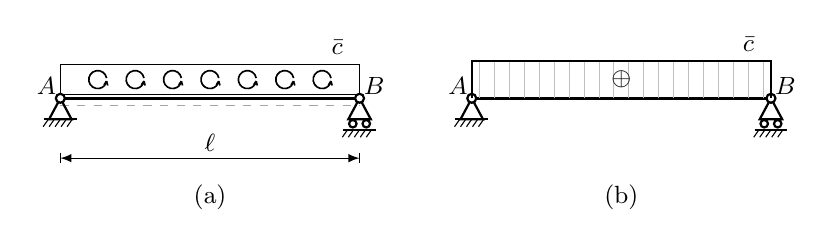
\begin{tikzpicture}[
					scale=0.95,
					>=latex,
					trave/.style={line width=1pt},
					carico/.style={black, line width=0.6pt},
					forza/.style={black, line width=1pt},
					diagT/.style={black, line width=0.8pt},
					hatch/.style={gray!50, line width=0.3pt},
					quota/.style={black, line width=0.4pt},
					fibre/.style={gray!70, line width=0.3pt},
					]
					
					% ── Parametri dei vincoli (convenzione C06/C07) ──
					\def\tw{0.15}    \def\thR{0.28}   \def\rn{0.06}
					\def\rw{0.05}    \def\bw{0.09}    \def\gw{0.22}
					\def\hh{0.10}
					
					% ── Geometria del problema ──
					\def\Lell{4}                            % lunghezza trave ℓ
					\pgfmathsetmacro{\xA}{0}
					\pgfmathsetmacro{\xMid}{0.5*\Lell}      % mezzeria
					\def\yqi{-0.80}                         % y delle quote sotto la trave
					\def\ylab{-3.30}                        % y delle etichette di pannello
					
					% ── Parametri del riquadro delle coppie distribuite ──
					\def\pgap{0.05}                         % gap fra trave e base del riquadro
					\def\php{0.40}                          % altezza del riquadro
					\pgfmathsetmacro{\pBase}{\pgap}         % base del riquadro: y = 0.05
					\pgfmathsetmacro{\pTop}{\pgap+\php}     % cima del riquadro: y = 0.45
					\pgfmathsetmacro{\pMid}{\pgap+0.5*\php} % centro del riquadro: y = 0.25
					\def\rCoppia{0.12}                      % raggio del singolo simbolo "coppia"
					
					% =========================================================
					% PANNELLO (a) — Schema statico
					% =========================================================
					\begin{scope}[xshift=0cm]
						
						% ── Trave ──
						\draw[trave] (0,0) -- (\Lell,0);
						
						% ── Fibra inferiore (tratteggio sotto la trave) ──
						\draw[fibre, dashed] (0, -0.1) -- (\Lell, -0.1);
						
						% ── Cerniera in A ──
						\draw[thick] (0,0) -- (-\tw,-\thR) -- (\tw,-\thR) -- cycle;
						\draw[thick] (-\gw,-\thR) -- (\gw,-\thR);
						\foreach \x in {-0.16,-0.08,0,0.08,0.16}
						\draw[thin] (\x,-\thR) -- ++(-0.07,-\hh);
						
						% ── Carrello verticale in B ──
						\draw[thick] (\Lell,0) -- (\Lell-\tw,-\thR) -- (\Lell+\tw,-\thR) -- cycle;
						\draw[thick] (\Lell-\bw,-\thR-\rw-0.01) circle (\rw);
						\draw[thick] (\Lell+\bw,-\thR-\rw-0.01) circle (\rw);
						\draw[thick] (\Lell-\gw,-\thR-2*\rw-0.04) -- (\Lell+\gw,-\thR-2*\rw-0.04);
						\foreach \x in {-0.16,-0.08,0,0.08,0.16}
						\draw[thin] (\Lell+\x,-\thR-2*\rw-0.04) -- ++(-0.07,-\hh);
						
						% ── Anellini bianchi sui perni ──
						\draw[thick, fill=white] (0,0) circle (\rn);
						\draw[thick, fill=white] (\Lell,0) circle (\rn);
						
						% ── Etichette A, B ──
						\node[above left=-2pt,  font=\small] at (0,0)      {$A$};
						\node[above right=-2pt, font=\small] at (\Lell,0)  {$B$};
						
						% ── Riquadro delle coppie distribuite ──
						\draw[carico] (0,\pBase) -- (\Lell,\pBase);
						\draw[carico] (0,\pTop)  -- (\Lell,\pTop);
						\draw[carico] (0,\pBase) -- (0,\pTop);
						\draw[carico] (\Lell,\pBase) -- (\Lell,\pTop);
						
						
						% ── Sette simboli "coppia antioraria" equispaziati ──
						\def\Lwing{0.06}    % lunghezza dell'ala della freccia
						\foreach \xs in {0.50, 1.00, 1.50, 2.00, 2.50, 3.00, 3.50} {
							% Arco quasi chiuso (340°, apertura 20°) — senza freccia automatica
							\draw[carico]
							({\xs+\rCoppia*cos(10)}, {\pMid+\rCoppia*sin(10)})
							arc[start angle=10, end angle=350, radius=\rCoppia];
							
							% Punta della freccia disegnata a due tratti, all'estremità a θ=350°
							\pgfmathsetmacro{\tipx}{\xs + \rCoppia*cos(350)}
							\pgfmathsetmacro{\tipy}{\pMid + \rCoppia*sin(350)}
							\draw[carico] (\tipx, \tipy)
							-- ({\tipx + \Lwing*cos(235)}, {\tipy + \Lwing*sin(235)});
							\draw[carico] (\tipx, \tipy)
							-- ({\tipx + \Lwing*cos(285)}, {\tipy + \Lwing*sin(285)});
						}
						
						% Etichetta c̄ sopra il riquadro, a destra
						\node[above, font=\small] at (\Lell-0.30, \pTop) {$\bar{c}$};
						
						% ── Quota ℓ sotto la trave ──
						\draw[<->, quota] (0,\yqi) -- (\Lell,\yqi);
						\draw[quota] (0,\yqi+0.07)     -- (0,\yqi-0.07);
						\draw[quota] (\Lell,\yqi+0.07) -- (\Lell,\yqi-0.07);
						\node[above, font=\small] at (\xMid, \yqi-0.04) {$\ell$};
						
						% Etichetta pannello (a)
						\node[font=\small] at (0.5*\Lell, 0.4*\ylab) {(a)};
						
					\end{scope}
					
					% =========================================================
					% PANNELLO (b) — Diagramma di T(z)
					% =========================================================
					\begin{scope}[xshift=5.5cm]
						
						% ── Trave (clone) ──
						\draw[trave] (0,0) -- (\Lell,0);
						
						% ── Vincoli (clone) ──
						\draw[thick] (0,0) -- (-\tw,-\thR) -- (\tw,-\thR) -- cycle;
						\draw[thick] (-\gw,-\thR) -- (\gw,-\thR);
						\foreach \x in {-0.16,-0.08,0,0.08,0.16}
						\draw[thin] (\x,-\thR) -- ++(-0.07,-\hh);
						\draw[thick] (\Lell,0) -- (\Lell-\tw,-\thR) -- (\Lell+\tw,-\thR) -- cycle;
						\draw[thick] (\Lell-\bw,-\thR-\rw-0.01) circle (\rw);
						\draw[thick] (\Lell+\bw,-\thR-\rw-0.01) circle (\rw);
						\draw[thick] (\Lell-\gw,-\thR-2*\rw-0.04) -- (\Lell+\gw,-\thR-2*\rw-0.04);
						\foreach \x in {-0.16,-0.08,0,0.08,0.16}
						\draw[thin] (\Lell+\x,-\thR-2*\rw-0.04) -- ++(-0.07,-\hh);
						\draw[thick, fill=white] (0,0) circle (\rn);
						\draw[thick, fill=white] (\Lell,0) circle (\rn);
						
						% ── Etichette A, B ──
						\node[above left=-2pt,  font=\small] at (0,0)      {$A$};
						\node[above right=-2pt, font=\small] at (\Lell,0)  {$B$};
						
						% ── Diagramma T(z) ──
						\def\sT{0.50}
						\pgfmathsetmacro{\Tval}{\sT}        % T(z) = +c̄ → +0.50
						
						% Hatching verticale uniforme su tutta la trave
						\foreach \x in {0.10, 0.30, ..., 3.90} {
							\draw[hatch] (\x, 0) -- (\x, \Tval);
						}
						
						% Bordo del diagramma — rettangolo
						\draw[diagT]
						(0, 0) -- (0, \Tval)             % verticale in A
						-- (\Lell, \Tval)                % uniforme su tutta la trave
						-- (\Lell, 0);                   % verticale di chiusura in B
						
						% Segno cerchiato al centro del rettangolo
						\node[font=\small] at (\xMid, {0.5*\Tval})
						{$\boldsymbol{\oplus}$};
						
						% Etichetta del valore c sopra il rettangolo, vicino al bordo destro
						\node[above, font=\small] at (\Lell-0.30, \Tval) {$\bar{c}$};
						
						% Etichetta pannello (b)
						\node[font=\small] at (0.5*\Lell, 0.4*\ylab) {(b)};
						
					\end{scope}
					
				\end{tikzpicture}
				%}
			\caption{Trave appoggiata con coppie antiorarie uniformemente
				distribuite di intensità $\bar{c}$ su tutta la lunghezza:
				(a)~schema strutturale;
				(b)~diagramma del taglio $T(z)$, uniforme pari a $\bar{c}$
				su tutta la trave.
				Il momento flettente è identicamente nullo, $M(z) \equiv 0$,
				e non è riportato in figura: le coppie distribuite
				compensano esattamente il contributo del taglio
				($M' = T - c = 0$).}
			\label{fig:stat_trasv_iso_06}
		\end{figure}
		
		
		
		\esottotit{Reazioni vincolari.}
		La cerniera in $A$ e il carrello verticale in $B$
		forniscono entrambi reazioni verticali; non vi
		sono carichi trasversali distribuiti ($p = 0$),
		ma solo coppie distribuite.
		Il sistema di coppie è equivalente a una coppia
		antioraria risultante di intensità $\bar{c}\ell$.
		Per equilibrio le reazioni devono formare una
		coppia oraria di uguale intensità: $V_A$ verso
		l'alto e $V_B$ verso il basso.
		Si assumono quindi $V_A$ positivo verso l'alto
		e $V_B$ positivo verso il basso.
		Dall'equilibrio globale:
		\[
		\sum \mu_A = 0:\quad
		-V_B\ell + \bar{c}\ell = 0
		\;\Rightarrow\;
		V_B = \bar{c},
		\]
		\[
		\sum V = 0:\quad
		V_A - V_B = 0
		\;\Rightarrow\;
		V_A = \bar{c}.
		\]
		
		\esottotit{Condizioni al contorno.}
		All'estremo $A$ (cerniera):
		\[
		T(A) = V_A = \bar{c}, \qquad M(A) = 0.
		\]
		All'estremo $B$ (carrello verticale, con $V_B$
		verso il basso, concorde con $+y^e$):
		\[
		T(B) = V_B = \bar{c}, \qquad M(B) = 0.
		\]
		
		\esottotit{Analisi qualitativa.}
		\begin{itemize}[nosep]
			\item su tutta la trave: $p = 0$, quindi
			$T' = 0$ e $T$ è \emph{uniforme};
			\item su tutta la trave: $c = \bar{c}$
			uniforme e $T$ uniforme, quindi
			$M' = T - c = \bar{c} - \bar{c} = 0$
			e $M$ è \emph{uniforme}; poiché
			$M(A) = M(B) = 0$, il momento è
			\emph{identicamente nullo}.
		\end{itemize}
		
		\esottotit{Diagramma del taglio.}
		
		Su tutta la trave, guardando a sinistra,
		$\mathcal{C}^-(z)$ contiene la sola reazione
		$V_A$ (verso l'alto; le coppie distribuite non
		contribuiscono alla risultante delle forze):
		\[
		T(z) = V_A = \bar{c}.
		\]
		Uniforme, in accordo con l'analisi qualitativa (\FIGref{fig:stat_trasv_iso_06}\,b).
		
		\esottotit{Diagramma del momento flettente.}
		
		Su tutta la trave, guardando a sinistra,
		$\mathcal{C}^-(z)$ contiene $V_A$ e le coppie
		distribuite su $[0,z]$, la cui risultante è
		$\bar{c}z$ antioraria:
		\[
		M(z) = V_A z - \bar{c}z = \bar{c}z - \bar{c}z = 0.
		\]
		Identicamente nullo, in accordo con l'analisi
		qualitativa.
		
		\esottotit{Lettura per aree.}
		La relazione $\dd M = (T - c)\,\dd z$ con $T = \bar{c}$
		e $c = \bar{c}$ dà $dM = 0$: la variazione di $M$
		è nulla su tutta la trave, confermando
		$M(z) \equiv 0$. $\quad\checkmark$
		
		\noindent
		Le coppie distribuite compensano esattamente
		il contributo del taglio al momento flettente:
		benché $T \neq 0$, si ha $M' = T - c = 0$ su
		tutta la trave. Il diagramma di $T(z)$ è uniforme
		pari a $\bar{c}$; il momento flettente è
		identicamente nullo, $M(z) \equiv 0$, e non
		viene riportato in figura.
		
	\end{svolgimento}
\end{esempio}


\begin{esempio}[Trave appoggiata con coppie concentrate alle estremità]
	Si consideri una trave piana di lunghezza $\ell$
	con cerniera in $A$ e carrello verticale in $B$,
	soggetta a coppie concentrate antiorarie
	$\mu(A)$ in $A$ e $\mu(B)$ in $B$ (\FIGref{fig:stat_trasv_iso_07}\,a).
	Si costruiscano i diagrammi quotati del taglio $T(z)$
	e del momento flettente $M(z)$.
	
	\begin{svolgimento}
		
		\begin{figure}[htbp]
			\centering
			\resizebox{\textwidth}{!}{%
				\begin{tikzpicture}[
					scale=0.95,
					>=latex,
					trave/.style={line width=1.4pt},
					carico/.style={black, line width=0.6pt},
					forza/.style={black, line width=0.8pt},
					diagT/.style={black, line width=0.6pt},
					diagM/.style={black, line width=0.6pt},
					hatch/.style={gray!50, line width=0.3pt},
					quota/.style={black, line width=0.4pt},
					fibre/.style={gray!70, line width=0.3pt},
					]
					
					% ── Parametri dei vincoli (convenzione C06/C07) ──
					\def\tw{0.15}    \def\thR{0.28}   \def\rn{0.06}
					\def\rw{0.05}    \def\bw{0.09}    \def\gw{0.22}
					\def\hh{0.10}
					
					% ── Geometria del problema ──
					\def\Lell{4}                            % lunghezza trave ℓ
					\pgfmathsetmacro{\xA}{0}
					\pgfmathsetmacro{\xMid}{0.5*\Lell}      % mezzeria

					\pgfmathsetmacro{\xZstar}{\Lell/3}
					\def\yqi{-0.80}                         % y delle quote sotto la trave
					\def\ylab{-3.30}                        % y delle etichette di pannello
					
					% ── Parametri del simbolo "coppia concentrata" ──
					\def\rCoppia{0.25}    % raggio dell'arco
					\def\Lwing{0.08}      % lunghezza dell'ala della freccia
					
					% =========================================================
					% PANNELLO (a) — Schema statico
					% =========================================================
					\begin{scope}[xshift=0cm]
						
						% ── Trave ──
						\draw[trave] (0,0) -- (\Lell,0);
						
						% ── Fibra inferiore (tratteggio sotto la trave) ──
						\draw[fibre, dashed] (0, -0.1) -- (\Lell, -0.1);
						
						% ── Cerniera in A ──
						\draw[thick] (0,0) -- (-\tw,-\thR) -- (\tw,-\thR) -- cycle;
						\draw[thick] (-\gw,-\thR) -- (\gw,-\thR);
						\foreach \x in {-0.16,-0.08,0,0.08,0.16}
						\draw[thin] (\x,-\thR) -- ++(-0.07,-\hh);
						
						% ── Carrello verticale in B ──
						\draw[thick] (\Lell,0) -- (\Lell-\tw,-\thR) -- (\Lell+\tw,-\thR) -- cycle;
						\draw[thick] (\Lell-\bw,-\thR-\rw-0.01) circle (\rw);
						\draw[thick] (\Lell+\bw,-\thR-\rw-0.01) circle (\rw);
						\draw[thick] (\Lell-\gw,-\thR-2*\rw-0.04) -- (\Lell+\gw,-\thR-2*\rw-0.04);
						\foreach \x in {-0.16,-0.08,0,0.08,0.16}
						\draw[thin] (\Lell+\x,-\thR-2*\rw-0.04) -- ++(-0.07,-\hh);
						
						% ── Anellini bianchi sui perni ──
						\draw[thick, fill=white] (0,0) circle (\rn);
						\draw[thick, fill=white] (\Lell,0) circle (\rn);
						
						% ── Etichette A, B (ancorate sotto, perché sopra c'è la coppia) ──
						\node[above left=-2pt,  font=\small] at (0,0)      {$A$};
						\node[above right=-2pt, font=\small] at (\Lell,0)  {$B$};
						
						% ── Parametri del simbolo "coppia concentrata" ──
						\def\rCoppia{0.25}    % raggio dell'arco
						\def\Lwing{0.12}      % lunghezza dell'ala della freccia (era 0.08)
						
						\def\AoffX{0.20}    % offset orizzontale del semicerchio di μ_A (verso destra)
						\def\BoffX{0.20}    % offset orizzontale del semicerchio di μ_B (verso sinistra)
						
						% ── Coppia antioraria in A: semicerchio sul lato DESTRO che attraversa la trave ──
						\draw[forza](\AoffX, -\rCoppia)
						arc[start angle=-90, end angle=90, radius=\rCoppia];
						% Punta della freccia all'estremità superiore (a +90°): punta verso sinistra
						\pgfmathsetmacro{\tipxA}{\AoffX}
						\pgfmathsetmacro{\tipyA}{\rCoppia}
						\draw[forza] (\tipxA, \tipyA)
						-- ({\tipxA + \Lwing*cos(25)},  {\tipyA + \Lwing*sin(25)});
						\draw[forza] (\tipxA, \tipyA)
						-- ({\tipxA + \Lwing*cos(-25)}, {\tipyA + \Lwing*sin(-25)});
						\node[right, font=\footnotesize] at ({\AoffX-\rCoppia+0.3}, 0.3) {$\mu_A$};
						
						
						% ── Coppia antioraria in B: semicerchio sul lato SINISTRO che attraversa la trave ──
						\draw[forza](\Lell-\BoffX, \rCoppia)
						arc[start angle=90, end angle=270, radius=\rCoppia];
						\pgfmathsetmacro{\tipxB}{\Lell-\BoffX}
						\pgfmathsetmacro{\tipyB}{-\rCoppia}
						\draw[forza] (\tipxB, \tipyB)
						-- ({\tipxB + \Lwing*cos(155)}, {\tipyB + \Lwing*sin(155)});
						\draw[forza] (\tipxB, \tipyB)
						-- ({\tipxB + \Lwing*cos(205)}, {\tipyB + \Lwing*sin(205)});
						\node[left, font=\footnotesize] at ({\Lell-\BoffX+\rCoppia-0.3}, 0.3) {$\mu_B$};
						
						
						% ── Quota ℓ sotto la trave ──
						\draw[<->, quota] (0,\yqi) -- (\Lell,\yqi);
						\draw[quota] (0,\yqi+0.07)     -- (0,\yqi-0.07);
						\draw[quota] (\Lell,\yqi+0.07) -- (\Lell,\yqi-0.07);
						\node[above, font=\small] at (\xMid, \yqi-0.04) {$\ell$};
						
						% Etichetta pannello (a)
						\node[font=\small] at (0.5*\Lell, 0.4*\ylab) {(a)};
						
					\end{scope}
					
					% =========================================================
					% PANNELLO (b) — Diagramma di T(z)
					% =========================================================
					\begin{scope}[xshift=5.5cm]
						
						% ── Trave (clone) ──
						\draw[trave] (0,0) -- (\Lell,0);
						
						% ── Vincoli (clone) ──
						\draw[thick] (0,0) -- (-\tw,-\thR) -- (\tw,-\thR) -- cycle;
						\draw[thick] (-\gw,-\thR) -- (\gw,-\thR);
						\foreach \x in {-0.16,-0.08,0,0.08,0.16}
						\draw[thin] (\x,-\thR) -- ++(-0.07,-\hh);
						\draw[thick] (\Lell,0) -- (\Lell-\tw,-\thR) -- (\Lell+\tw,-\thR) -- cycle;
						\draw[thick] (\Lell-\bw,-\thR-\rw-0.01) circle (\rw);
						\draw[thick] (\Lell+\bw,-\thR-\rw-0.01) circle (\rw);
						\draw[thick] (\Lell-\gw,-\thR-2*\rw-0.04) -- (\Lell+\gw,-\thR-2*\rw-0.04);
						\foreach \x in {-0.16,-0.08,0,0.08,0.16}
						\draw[thin] (\Lell+\x,-\thR-2*\rw-0.04) -- ++(-0.07,-\hh);
						\draw[thick, fill=white] (0,0) circle (\rn);
						\draw[thick, fill=white] (\Lell,0) circle (\rn);
						
						% ── Etichette A, B ──
						\node[above left=-2pt,  font=\small] at (0,0)      {$A$};
						\node[above right=-2pt, font=\small] at (\Lell,0)  {$B$};
						
						% ── Diagramma T(z) ──   QUI HO FATTO CASINO!!!!
						\def\sT{0.67}
						\pgfmathsetmacro{\Tval}{(3/\Lell)*\sT}    % T(z) = 3/ℓ → 0.75·0.67 ≈ 0.50
						
						% Hatching verticale uniforme su tutta la trave
						\foreach \x in {0.10, 0.30, ..., 3.90} {
							\draw[hatch] (\x, 0) -- (\x, \Tval);
						}
						
						% Bordo del diagramma — rettangolo
						\draw[diagT]
						(0, 0) -- (0, \Tval)             % verticale in A
						-- (\Lell, \Tval)                % uniforme su tutta la trave
						-- (\Lell, 0);                   % verticale di chiusura in B
						
						% Segno cerchiato al centro del rettangolo
						\node[font=\small] at (\xMid, {0.5*\Tval})	{$\boldsymbol{\oplus}$};
						
						% Etichetta del valore (μ_A+μ_B)/ℓ sopra il rettangolo, a destra
						\node[above, font=\small] at (\Lell-0.3, \Tval)	{$\tfrac{\mu_A + \mu_B}{\ell}$};
						
						% Etichetta pannello (b)
						\node[font=\small] at (0.5*\Lell, 0.4*\ylab) {(b)};
						
					\end{scope}
					
					% =========================================================
					% PANNELLO (c) — Diagramma di M(z)
					% =========================================================
					\begin{scope}[xshift=11.0cm]
						
						% ── Trave (clone) ──
						\draw[trave] (0,0) -- (\Lell,0);
						
						% ── Vincoli (clone) ──
						\draw[thick] (0,0) -- (-\tw,-\thR) -- (\tw,-\thR) -- cycle;
						\draw[thick] (-\gw,-\thR) -- (\gw,-\thR);
						\foreach \x in {-0.16,-0.08,0,0.08,0.16}
						\draw[thin] (\x,-\thR) -- ++(-0.07,-\hh);
						\draw[thick] (\Lell,0) -- (\Lell-\tw,-\thR) -- (\Lell+\tw,-\thR) -- cycle;
						\draw[thick] (\Lell-\bw,-\thR-\rw-0.01) circle (\rw);
						\draw[thick] (\Lell+\bw,-\thR-\rw-0.01) circle (\rw);
						\draw[thick] (\Lell-\gw,-\thR-2*\rw-0.04) -- (\Lell+\gw,-\thR-2*\rw-0.04);
						\foreach \x in {-0.16,-0.08,0,0.08,0.16}
						\draw[thin] (\Lell+\x,-\thR-2*\rw-0.04) -- ++(-0.07,-\hh);
						\draw[thick, fill=white] (0,0) circle (\rn);
						\draw[thick, fill=white] (\Lell,0) circle (\rn);
						
						% ── Etichette A, B ──
						\node[above left=-2pt,  font=\small] at (0,0)      {$A$};
						\node[above right=-2pt, font=\small] at (\Lell,0)  {$B$};
						
						% ── Punto z* dove M=0 ──
						\draw[forza] (\xZstar, -0.10) -- (\xZstar, 0.10);
						
						% ── Diagramma M(z) ──
						\def\sM{0.50}
						\pgfmathsetmacro{\MAfig}{ 1*\sM}      % M(A) = -μ_A = -1 → sopra: +0.40
						\pgfmathsetmacro{\MBfig}{-2*\sM}      % M(B) = +μ_B = +2 → sotto: -0.80
						
						% Hatching tratto [0, z*]: lineare, sopra l'asse (M<0)
						\foreach \x in {0.10, 0.30, ..., 1.30} {
							\pgfmathsetmacro{\h}{\MAfig*(1 - \x/\xZstar)}
							\draw[hatch] (\x, 0) -- (\x, \h);
						}
						% Hatching tratto [z*, ℓ]: lineare, sotto l'asse (M>0)
						\foreach \x in {1.50, 1.70, ..., 3.90} {
							\pgfmathsetmacro{\h}{\MBfig*(\x - \xZstar)/(\Lell - \xZstar)}
							\draw[hatch] (\x, 0) -- (\x, \h);
						}
						
						% Bordo del diagramma — retta da (0, MAfig) a (ℓ, MBfig), con chiusure verticali agli estremi
						\draw[diagM]
						(0, 0) -- (0, \MAfig)            % verticale di chiusura in A
						-- (\Lell, \MBfig)               % retta attraverso lo zero in z*
						-- (\Lell, 0);                   % verticale di chiusura in B
						
						% Etichette dei valori notevoli
						% μ_A: sopra il vertice in A (lobo negativo)
						\node[above, font=\small] at (0, \MAfig+0.04) {$\mu_A$};
						% μ_B: sotto il vertice in B (lobo positivo)
						\node[right, font=\small] at (\Lell, \MBfig-0.04) {$\mu_B$};
						% z* sotto la tacca
						\node[below, font=\footnotesize] at (\xZstar, -0.12) {$z^*$};
						
						% Etichetta pannello (c)
						\node[font=\small] at (0.5*\Lell, 0.4*\ylab) {(c)};
						
					\end{scope}
					
				\end{tikzpicture}
			}
			\caption{Trave appoggiata con coppie concentrate antiorarie
				$\mu_A$ in $A$ e $\mu_B$ in $B$:
				(a)~schema strutturale;
				(b)~diagramma del taglio $T(z)$, uniforme pari a
				$(\mu_A + \mu_B)/\ell$ su tutta la trave;
				(c)~diagramma del momento flettente $M(z)$, lineare
				crescente da $-\mu_A$ in $A$ a $\mu_B$ in $B$, con
				annullamento in $z^* = \mu_A\ell/(\mu_A+\mu_B)$.}
			\label{fig:stat_trasv_iso_07}
		\end{figure}
		

		
		\esottotit{Reazioni vincolari.}
		Non vi sono carichi trasversali distribuiti
		($p = 0$) né coppie distribuite ($c = 0$).
		Il sistema di coppie concentrate è equivalente
		a una coppia antioraria risultante di intensità
		$\mu(A) + \mu(B)$. Per equilibrio le reazioni
		devono formare una coppia oraria di uguale
		intensità: $V_A$ verso l'alto e $V_B$ verso
		il basso.
		Si assumono quindi $V_A$ positivo verso l'alto
		e $V_B$ positivo verso il basso.
		Dall'equilibrio globale:
		\[
		\sum \mu_A = 0:\quad
		-V_B\ell + \mu(A) + \mu(B) = 0
		\;\Rightarrow\;
		V_B = \frac{\mu(A) + \mu(B)}{\ell},
		\]
		\[
		\sum V = 0:\quad
		V_A - V_B = 0
		\;\Rightarrow\;
		V_A = \frac{\mu(A) + \mu(B)}{\ell}.
		\]
		
		\esottotit{Condizioni al contorno.}
		All'estremo $A$ (cerniera): la coppia $\mu(A)$
		antioraria è discorde con il verso positivo di
		$M$ sulla faccia sinistra; pertanto:
		\[
		T(A) = V_A = \frac{\mu(A)+\mu(B)}{\ell},
		\qquad
		M(A) = -\mu(A).
		\]
		All'estremo $B$ (carrello verticale, con $V_B$
		verso il basso concorde con $+y^e$, e $\mu(B)$
		antioraria concorde con il verso positivo di $M$
		sulla faccia destra):
		\[
		T(B) = V_B = \frac{\mu(A)+\mu(B)}{\ell},
		\qquad
		M(B) = \mu(B).
		\]
		
		\esottotit{Analisi qualitativa.}
		\begin{itemize}[nosep]
			\item su tutta la trave: $p = 0$, quindi
			$T' = 0$ e $T$ è \emph{uniforme};
			\item su tutta la trave: $c = 0$ e $T$
			uniforme, quindi $M' = T$ uniforme
			e $M$ è \emph{lineare};
			\item non vi sono forze o coppie concentrate
			nei punti interni, quindi $T$ e $M$
			sono continui su $(0,\ell)$.
		\end{itemize}
		
		\esottotit{Diagramma del taglio.}
		
		Su tutta la trave $(0 \leq z \leq \ell)$,
		guardando a sinistra, $\mathcal{C}^-(z)$ contiene
		la sola reazione $V_A$ (le coppie concentrate
		agli estremi non contribuiscono alla risultante
		delle forze):
		\[
		T(z) = V_A = \frac{\mu(A)+\mu(B)}{\ell}.
		\]
		Uniforme, in accordo con l'analisi qualitativa.
		
		\esottotit{Diagramma del momento flettente.}
		
		Su tutta la trave $(0 \leq z \leq \ell)$,
		guardando a sinistra, $\mathcal{C}^-(z)$ contiene
		$V_A$ e la coppia $\mu(A)$ antioraria (discorde
		con il verso positivo di $M$):
		\[
		M(z) = -\mu(A) + V_A z
		= -\mu(A) + \frac{\mu(A)+\mu(B)}{\ell}z.
		\]
		Lineare crescente da $M(0) = -\mu(A)$ a
		$M(\ell) = \mu(B)$, in accordo con le condizioni
		al contorno.
		
		\esottotit{Lettura per aree.}
		La relazione $\dd M = T\,\dd z$ (con $c = 0$) dà:
		\[
		M(\ell) - M(0) = T \cdot \ell
		= \frac{\mu(A)+\mu(B)}{\ell}\cdot\ell
		= \mu(A)+\mu(B).
		\]
		Verifica: $M(\ell) - M(0) = \mu(B) -(-\mu(A))
		= \mu(A)+\mu(B)$. $\quad\checkmark$
		
		\noindent
		Il diagramma di $T(z)$ è uniforme pari a
		$[\mu(A)+\mu(B)]/\ell$ (\FIGref{fig:stat_trasv_iso_07}\,b).
		Il diagramma di $M(z)$ è lineare crescente
		da $-\mu(A)$ in $A$ a $\mu(B)$ in $B$;
		il punto di annullamento di $M$ è in
		$z^* = \mu(A)\ell/[\mu(A)+\mu(B)]$ (\FIGref{fig:stat_trasv_iso_07}\,c).
		
	\end{svolgimento}
\end{esempio}


\begin{esempio}[Trave appoggiata con coppia concentrata intermedia]
	Si consideri una trave piana di lunghezza $\ell$
	con cerniera in $A$ e carrello verticale in $B$,
	soggetta a una coppia concentrata antioraria di
	intensità $\mu$ applicata nel punto $C$ a
	distanza $\ell/3$ da $A$ (\FIGref{fig:stat_trasv_iso_08}\,a).
	Si costruiscano i diagrammi quotati del taglio $T(z)$
	e del momento flettente $M(z)$.
	
	\begin{svolgimento}
		
		
		\begin{figure}[htbp]
			\centering
			\resizebox{\textwidth}{!}{%
				\begin{tikzpicture}[
					scale=0.95,
					>=latex,
					trave/.style={line width=1.4pt},
					carico/.style={black, line width=0.6pt},
					forza/.style={black, line width=0.7pt},
					diagT/.style={black, line width=0.8pt},
					diagM/.style={black, line width=0.8pt},
					hatch/.style={gray!50, line width=0.3pt},
					quota/.style={black, line width=0.2pt},
					fibre/.style={gray!70, line width=0.3pt},
					]
					
					% ── Parametri dei vincoli (convenzione C06/C07) ──
					\def\tw{0.15}    \def\thR{0.28}   \def\rn{0.06}
					\def\rw{0.05}    \def\bw{0.09}    \def\gw{0.22}
					\def\hh{0.10}
					
					% ── Geometria del problema ──
					\def\Lell{4}                            % lunghezza trave ℓ
					\pgfmathsetmacro{\xA}{0}
					\pgfmathsetmacro{\xC}{\Lell/3}          % C a ℓ/3 da A ≈ 1.333
					\def\yqi{-0.80}                         % y delle quote sotto la trave
					\def\ylab{-3.30}                        % y delle etichette di pannello
					
					% ── Centri di tratto utili per le etichette ──
					\pgfmathsetmacro{\xMidAC}{0.5*\xC}      % centro tratto AC
					
					% ── Parametri del simbolo "coppia concentrata" ──
					\def\rCoppia{0.25}    % raggio dell'arco
					\def\Lwing{0.12}      % lunghezza dell'ala della freccia
					\def\Lstem{0.05}      % lunghezza del tratto rettilineo (stelo) dal sud dell'arco al punto C
					
					% =========================================================
					% PANNELLO (a) — Schema statico
					% =========================================================
					\begin{scope}[xshift=0cm]
						
						% ── Trave ──
						\draw[trave] (0,0) -- (\Lell,0);
						
						% ── Fibra inferiore (tratteggio sotto la trave) ──
						\draw[fibre, dashed] (0, -0.1) -- (\Lell, -0.1);
						
						% ── Cerniera in A ──
						\draw[thick] (0,0) -- (-\tw,-\thR) -- (\tw,-\thR) -- cycle;
						\draw[thick] (-\gw,-\thR) -- (\gw,-\thR);
						\foreach \x in {-0.16,-0.08,0,0.08,0.16}
						\draw[thin] (\x,-\thR) -- ++(-0.07,-\hh);
						
						% ── Carrello verticale in B ──
						\draw[thick] (\Lell,0) -- (\Lell-\tw,-\thR) -- (\Lell+\tw,-\thR) -- cycle;
						\draw[thick] (\Lell-\bw,-\thR-\rw-0.01) circle (\rw);
						\draw[thick] (\Lell+\bw,-\thR-\rw-0.01) circle (\rw);
						\draw[thick] (\Lell-\gw,-\thR-2*\rw-0.04) -- (\Lell+\gw,-\thR-2*\rw-0.04);
						\foreach \x in {-0.16,-0.08,0,0.08,0.16}
						\draw[thin] (\Lell+\x,-\thR-2*\rw-0.04) -- ++(-0.07,-\hh);
						
						% ── Anellini bianchi sui perni ──
						\draw[thick, fill=white] (0,0) circle (\rn);
						\draw[thick, fill=white] (\Lell,0) circle (\rn);
						
						% ── Etichette A, B ──
						\node[above left=-2pt,  font=\small] at (0,0)      {$A$};
						\node[above right=-2pt, font=\small] at (\Lell,0)  {$B$};
						
						
						% ── Stelo verticale: dal punto sud del semicerchio al punto C sulla trave ──
						\draw[forza] (\xC, -\rCoppia) -- (\xC, 0);
						
						% ── Coppia antioraria μ in C ──
						\draw[forza]
						(\xC, -\rCoppia)
						arc[start angle=-90, end angle=90, radius=\rCoppia];
						% Punta della freccia all'estremità superiore: punta verso sinistra
						\pgfmathsetmacro{\tipxC}{\xC}
						\pgfmathsetmacro{\tipyC}{\rCoppia}
						\draw[forza] (\tipxC, \tipyC)
						-- ({\tipxC + \Lwing*cos(25)},  {\tipyC + \Lwing*sin(25)});
						\draw[forza] (\tipxC, \tipyC)
						-- ({\tipxC + \Lwing*cos(-25)}, {\tipyC + \Lwing*sin(-25)});
						% Etichetta μ in alto a sinistra del simbolo
						\node[left, font=\small] at (\xC - 0.05, \rCoppia) {$\mu$};
						
						% ── Quote ℓ/3 (da A a C) e 2ℓ/3 (da C a B) sotto la trave ──
						\draw[<->, quota] (0,\yqi)   -- (\xC,\yqi);
						\draw[<->, quota] (\xC,\yqi) -- (\Lell,\yqi);
						\draw[quota] (0,\yqi+0.07)     -- (0,\yqi-0.07);
						\draw[quota] (\xC,\yqi+0.07)   -- (\xC,\yqi-0.07);
						\draw[quota] (\Lell,\yqi+0.07) -- (\Lell,\yqi-0.07);
						\pgfmathsetmacro{\xMidCB}{0.5*(\xC+\Lell)}    % centro del tratto CB
						\node[above, font=\footnotesize] at (\xMidAC, \yqi-0.1) {$\ell/3$};
						\node[above, font=\footnotesize] at (\xMidCB, \yqi-0.1) {$2\ell/3$};
						
						% Etichetta pannello (a)
						\node[font=\small] at (0.5*\Lell, 0.4*\ylab) {(a)};
						
					\end{scope}
					
					% =========================================================
					% PANNELLO (b) — Diagramma di T(z)
					% =========================================================
					\begin{scope}[xshift=5.5cm]
						
						% ── Trave (clone) ──
						\draw[trave] (0,0) -- (\Lell,0);
						
						% ── Vincoli (clone) ──
						\draw[thick] (0,0) -- (-\tw,-\thR) -- (\tw,-\thR) -- cycle;
						\draw[thick] (-\gw,-\thR) -- (\gw,-\thR);
						\foreach \x in {-0.16,-0.08,0,0.08,0.16}
						\draw[thin] (\x,-\thR) -- ++(-0.07,-\hh);
						\draw[thick] (\Lell,0) -- (\Lell-\tw,-\thR) -- (\Lell+\tw,-\thR) -- cycle;
						\draw[thick] (\Lell-\bw,-\thR-\rw-0.01) circle (\rw);
						\draw[thick] (\Lell+\bw,-\thR-\rw-0.01) circle (\rw);
						\draw[thick] (\Lell-\gw,-\thR-2*\rw-0.04) -- (\Lell+\gw,-\thR-2*\rw-0.04);
						\foreach \x in {-0.16,-0.08,0,0.08,0.16}
						\draw[thin] (\Lell+\x,-\thR-2*\rw-0.04) -- ++(-0.07,-\hh);
						\draw[thick, fill=white] (0,0) circle (\rn);
						\draw[thick, fill=white] (\Lell,0) circle (\rn);
						
						% ── Etichette A, B ──
						\node[above left=-2pt,  font=\small] at (0,0)      {$A$};
						\node[above right=-2pt, font=\small] at (\Lell,0)  {$B$};
						
						% ── Tacca verticale in C ──
						\draw[forza] (\xC, -0.10) -- (\xC, 0.10);
						
						% ── Diagramma T(z) ──
						\def\sT{2.5}
						\pgfmathsetmacro{\Tval}{(1/\Lell)*\sT}    % T(z) = μ/ℓ = 1/ℓ → 0.25·2.0 = 0.50
						
						% Hatching verticale uniforme su tutta la trave
						\foreach \x in {0.10, 0.30, ..., 3.90} {
							\draw[hatch] (\x, 0) -- (\x, \Tval);
						}
						
						% Bordo del diagramma — rettangolo
						\draw[diagT]
						(0, 0) -- (0, \Tval)             % verticale in A
						-- (\Lell, \Tval)                % uniforme su tutta la trave
						-- (\Lell, 0);                   % verticale di chiusura in B
						
						% Segno cerchiato al centro del rettangolo
						\node[font=\small] at (0.5*\Lell, {0.5*\Tval})
						{$\boldsymbol{\oplus}$};
						
						% Etichetta del valore μ/ℓ sopra il rettangolo, a destra
						\node[above, font=\small] at (\Lell-0.30, \Tval) {$\tfrac{\mu}{\ell}$};
						
						% Etichetta pannello (b)
						\node[font=\small] at (0.5*\Lell, 0.4*\ylab) {(b)};
						
					\end{scope}
					
					% =========================================================
					% PANNELLO (c) — Diagramma di M(z)
					% =========================================================
					\begin{scope}[xshift=11.0cm]
						
						% ── Trave (clone) ──
						\draw[trave] (0,0) -- (\Lell,0);
						
						% ── Vincoli (clone) ──
						\draw[thick] (0,0) -- (-\tw,-\thR) -- (\tw,-\thR) -- cycle;
						\draw[thick] (-\gw,-\thR) -- (\gw,-\thR);
						\foreach \x in {-0.16,-0.08,0,0.08,0.16}
						\draw[thin] (\x,-\thR) -- ++(-0.07,-\hh);
						\draw[thick] (\Lell,0) -- (\Lell-\tw,-\thR) -- (\Lell+\tw,-\thR) -- cycle;
						\draw[thick] (\Lell-\bw,-\thR-\rw-0.01) circle (\rw);
						\draw[thick] (\Lell+\bw,-\thR-\rw-0.01) circle (\rw);
						\draw[thick] (\Lell-\gw,-\thR-2*\rw-0.04) -- (\Lell+\gw,-\thR-2*\rw-0.04);
						\foreach \x in {-0.16,-0.08,0,0.08,0.16}
						\draw[thin] (\Lell+\x,-\thR-2*\rw-0.04) -- ++(-0.07,-\hh);
						\draw[thick, fill=white] (0,0) circle (\rn);
						\draw[thick, fill=white] (\Lell,0) circle (\rn);
						
						% ── Etichette A, B ──
						\node[above left=-2pt,  font=\small] at (0,0)      {$A$};
						\node[above right=-2pt, font=\small] at (\Lell,0)  {$B$};
						
						% ── Tacca verticale in C ──
						\draw[forza] (\xC, -0.10) -- (\xC, 0.10);
						
						% ── Diagramma M(z) ──
						\def\sM{1.4}
						\pgfmathsetmacro{\McMinus}{-(1/3)*\sM}    % M(C⁻) = +μ/3 → sotto: -0.40
						\pgfmathsetmacro{\McPlus}{ (2/3)*\sM}     % M(C⁺) = -2μ/3 → sopra: +0.80
						
						% Hatching tratto AC: lineare, sotto l'asse (M>0)
						\foreach \x in {0.10, 0.30, ..., 1.30} {
							\pgfmathsetmacro{\h}{\McMinus*\x/\xC}
							\draw[hatch] (\x, 0) -- (\x, \h);
						}
						% Hatching tratto CB: lineare, sopra l'asse (M<0)
						\foreach \x in {1.50, 1.70, ..., 3.90} {
							\pgfmathsetmacro{\h}{\McPlus*(\Lell-\x)/(\Lell-\xC)}
							\draw[hatch] (\x, 0) -- (\x, \h);
						}
						
						% Bordo del diagramma — due segmenti lineari + salto verticale in C
						\draw[diagM]
						(0, 0) -- (\xC, \McMinus)         % retta da A a C⁻ (sotto)
						-- (\xC, \McPlus)                 % salto verticale in C (attraversa l'asse)
						-- (\Lell, 0);                    % retta da C⁺ a B (sopra)
						
						% Etichette dei valori notevoli
						\node[right, font=\small] at (\xC, \McMinus-0.04)	{$\tfrac{\mu}{3}$};
						% 2μ/3 sopra il vertice in C⁺ (lobo negativo, sopra l'asse)
						\node[left, font=\small] at (\xC, \McPlus+0.04){$\tfrac{2\mu}{3}$};
						
						% Etichetta pannello (c)
						\node[font=\small] at (0.5*\Lell, 0.4*\ylab) {(c)};
						
					\end{scope}
					
				\end{tikzpicture}
			}
			\caption{Trave appoggiata con coppia concentrata antioraria $\mu$
				applicata in $C$ a distanza $\ell/3$ da $A$:
				(a)~schema strutturale;
				(b)~diagramma del taglio $T(z)$, uniforme pari a $\mu/\ell$
				su tutta la trave (la coppia concentrata non produce salto
				del taglio);
				(c)~diagramma del momento flettente $M(z)$, lineare crescente
				a tratti, da $0$ a $\mu/3$ in $AC$ e da $-2\mu/3$ a $0$
				in $CB$, con salto $-\mu$ in $C$.}
			\label{fig:stat_trasv_iso_08}
		\end{figure}
		
		
		\esottotit{Reazioni vincolari.}
		Non vi sono carichi trasversali distribuiti
		($p = 0$) né coppie distribuite ($c = 0$).
		La coppia concentrata $\mu$ è antioraria
		e applicata nel punto interno $C$. Per equilibrio le reazioni devono
		formare una coppia oraria di uguale intensità:
		$V_A$ verso l'alto e $V_B$ verso il basso.
		Si assumono quindi $V_A$ positivo verso l'alto
		e $V_B$ positivo verso il basso.
		Dall'equilibrio globale:
		\[
		\sum \mu_A = 0:\quad
		-V_B\ell + \mu = 0
		\;\Rightarrow\;
		V_B = \frac{\mu}{\ell},
		\]
		\[
		\sum V = 0:\quad
		V_A - V_B = 0
		\;\Rightarrow\;
		V_A = \frac{\mu}{\ell}.
		\]
		
		\esottotit{Condizioni al contorno.}
		All'estremo $A$ (cerniera):
		\[
		T(A) = V_A = \frac{\mu}{\ell}, \qquad M(A) = 0.
		\]
		All'estremo $B$ (carrello verticale, con $V_B$
		verso il basso concorde con $+y^e$):
		\[
		T(B) = V_B = \frac{\mu}{\ell}, \qquad M(B) = 0.
		\]
		
		\esottotit{Analisi qualitativa.}
		\begin{itemize}[nosep]
			\item su tutta la trave: $p = 0$, quindi
			$T' = 0$ e $T$ è \emph{uniforme};
			la coppia concentrata in $C$ non
			produce salto del taglio, quindi $T$
			è \emph{continuo} su tutta la trave;
			\item nel tratto $AC$ e nel tratto $CB$:
			$c = 0$ e $T$ uniforme, quindi
			$M' = T$ uniforme e $M$ è
			\emph{lineare crescente} in
			ciascun tratto;
			\item in $C$: è applicata la coppia
			concentrata $\mu \neq 0$, quindi
			$M$ presenta un \emph{salto negativo}
			di ampiezza $\mu$.
		\end{itemize}
		
		\esottotit{Diagramma del taglio.}
		
		Su tutta la trave $(0 \leq z \leq \ell)$,
		guardando a sinistra, $\mathcal{C}^-(z)$ contiene
		la sola reazione $V_A$ (la coppia concentrata
		in $C$ non contribuisce alla risultante delle
		forze):
		\[
		T(z) = V_A = \frac{\mu}{\ell}.
		\]
		Uniforme su tutta la trave, in accordo con
		l'analisi qualitativa.
		
		\esottotit{Diagramma del momento flettente.}
		
		\textit{Tratto $AC$ $(0 \leq z \leq \ell/3)$:}
		Guardando a sinistra, $\mathcal{C}^-(z)$ contiene
		la sola reazione $V_A$:
		\[
		M(z) = V_A z = \frac{\mu}{\ell}z.
		\]
		Lineare crescente da $M(0) = 0$ a
		$M(\ell/3^-) = \mu/3$, in accordo con
		l'analisi qualitativa.
		
		\textit{Tratto $CB$ $(\ell/3 < z \leq \ell)$:}
		Guardando a destra, $\mathcal{C}^+(z)$ contiene
		$V_B$ (verso il basso, concorde con $+y^e$,
		a distanza $\ell-z$ dalla sezione) e la coppia
		$\mu$ antioraria; sulla faccia destra una
		coppia antioraria è discorde con il verso
		positivo di $M$, quindi entra con segno negativo:
		\[
		M(z) = -V_B(\ell-z) - \mu
		= -\frac{\mu}{\ell}(\ell-z) - \mu
		= \frac{\mu}{\ell}(z - \ell).
		\]
		Lineare crescente da $M(\ell/3^+) = -2\mu/3$
		a $M(\ell) = 0$, in accordo con l'analisi
		qualitativa.
		
		\esottotit{Verifica del salto in $C$:}
		\[
		M\!\left(\frac{\ell}{3}^+\right) -
		M\!\left(\frac{\ell}{3}^-\right)
		= -\frac{2\mu}{3} - \frac{\mu}{3}
		= -\mu. \quad\checkmark
		\]
		Il salto negativo è coerente: $\mu$ è
		antioraria, quindi sulla faccia sinistra è
		concorde con il verso positivo di $M$, e
		produce un salto negativo di $M$ nel passare
		da sinistra a destra di $C$.
		
		\esottotit{Lettura per aree.}
		La relazione $\dd M = T\,\dd z$ (con $c = 0$) nel
		tratto $AC$ dà:
		\[
		M(\ell/3^-) - M(0)
		= \frac{\mu}{\ell}\cdot\frac{\ell}{3}
		= \frac{\mu}{3}. \quad\checkmark
		\]
		Nel tratto $CB$:
		\[
		M(\ell) - M(\ell/3^+)
		= \frac{\mu}{\ell}\cdot\frac{2\ell}{3}
		= \frac{2\mu}{3}
		\;\Rightarrow\;
		M(\ell) = -\frac{2\mu}{3}
		+ \frac{2\mu}{3} = 0. \quad\checkmark
		\]
		
		\noindent
		Il diagramma di $T(z)$ è uniforme pari a
		$\mu/\ell$ su tutta la trave (\FIGref{fig:stat_trasv_iso_08}\,b).
		Il diagramma di $M(z)$ è lineare a tratti:
		crescente da $0$ a $\mu/3$ nel tratto $AC$,
		con salto negativo $-\mu$ in $C$, e
		nuovamente crescente da $-2\mu/3$ a $0$
		nel tratto $CB$ (\FIGref{fig:stat_trasv_iso_08}\,c).
		
	\end{svolgimento}
\end{esempio}


\subsection{Proprietà di tangenza del diagramma del momento}
\label{sec:tangenze_momento}

Due proprietà geometriche del diagramma del momento\index{tangenza del diagramma del momento|textbf}
flettente, indipendenti dalla particolare distribuzione
dei vincoli, permettono controlli qualitativi rapidi
del tracciamento e, attraverso il principio di
sovrapposizione degli effetti, consentono di scomporre
diagrammi complessi come somma di contributi
elementari (\FIGref{fig:stat_tangenze}).

\begin{figure}[htbp]
	\centering
	\resizebox{0.92\textwidth}{!}{%
		\begin{tikzpicture}[
			scale=1.0,
			>=latex,
			trave/.style={line width=1.2pt},
			diagM/.style={black, line width=0.8pt},
			diagMb/.style={gray!65, line width=1.0pt},
			hatch/.style={gray!40, line width=0.3pt},
			puntotang/.style={circle, fill=black, inner sep=1.2pt},
			richiamo/.style={gray!50!black, line width=0.3pt},
			]
			
			% ── Parametri geometrici (tratto generico [z_1, z_2]) ──
			\def\Ltratto{4}
			\pgfmathsetmacro{\xZ}{0}
			\pgfmathsetmacro{\xMid}{0.5*\Ltratto}
			\pgfmathsetmacro{\xZZ}{\Ltratto}
			
			% ── Scala verticale per ariosità ──
			\def\vscale{1.6}
			
			% Coordinate di disegno (conv. italiana: y_dis = -M)
			\pgfmathsetmacro{\yA}{0.5*\vscale}        % y_dis(z_1) = +0.5
			\pgfmathsetmacro{\yB}{-0.5*\vscale}       % y_dis(z_2) = -0.5
			\pgfmathsetmacro{\yMezz}{-0.4*\vscale}    % y_dis in mezzeria = -0.4
			\pgfmathsetmacro{\yRaccordo}{-0.8*\vscale}% y_dis vertice spezzata
			\pgfmathsetmacro{\yTangA}{0.1*\vscale}    % y_dis tangente parallela in z_1
			\pgfmathsetmacro{\yTangB}{-0.9*\vscale}   % y_dis tangente parallela in z_2
			\def\ylab{-1.95}
			
			% =========================================================
			% PANNELLO (a) — Tangenza agli estremi
			% =========================================================
			\begin{scope}[xshift=0cm]
				
				\draw[trave] (\xZ, 0) -- (\xZZ, 0);
				\node[below=2pt, font=\small] at (\xZ, 0) {$z_1$};
				\node[below=2pt, font=\small] at (\xZZ, 0) {$z_2$};
				\node[below=2pt, font=\small] at (\xMid, 0) {$z_G$};
				
				% Hatching della parabola
				\foreach \x in {0.10, 0.30, ..., 3.90} {
					\pgfmathsetmacro{\h}{(0.10*\x*\x - 0.65*\x + 0.5)*\vscale}
					\draw[hatch] (\x, 0) -- (\x, \h);
				}
				
				% Verticale di allineamento: baricentro z_G ↔ vertice della spezzata
				\draw[richiamo, dashed] (\xMid, 0) -- (\xMid, \yRaccordo);
				
				% Spezzata di sostituzione (caso b)
				\draw[diagMb]
				(\xZ, \yA) -- (\xMid, \yRaccordo) -- (\xZZ, \yB);
				
				% Parabola del momento (caso a)
				\draw[diagM]
				(\xZ, \yA)
				\foreach \x in {0.20, 0.40, ..., 3.80} {
					-- ({\x}, {(0.10*\x*\x - 0.65*\x + 0.5)*\vscale})
				}
				-- (\xZZ, \yB);
				
				% Punti di tangenza (cerchietti pieni agli estremi)
				\node[puntotang] at (\xZ, \yA) {};
				\node[puntotang] at (\xZZ, \yB) {};
				
				% Etichette dei valori del momento agli estremi
				\node[left=2pt, font=\small] at (\xZ, \yA) {$M(z_1)$};
				\node[right=2pt, font=\small] at (\xZZ, \yB) {$M(z_2)$};
				
				% Etichetta della parabola (sopra l'asse, agganciata alla curva)
				\draw[richiamo] (2.6, -0.82) -- (2.6, 0.45);
				\node[above, font=\footnotesize] at (2.6, 0.45) {parabola $M(z)$};
				
				% Etichetta della spezzata di sostituzione
				\draw[richiamo] (\xMid, \yRaccordo) -- (\xMid+0.9, \yRaccordo-0.35);
				\node[right, font=\footnotesize, gray!50!black]
				at (\xMid+0.9, \yRaccordo-0.35) {spezzata di sostituzione};
				
			\end{scope}
			
			% =========================================================
			% PANNELLO (b) — Tangenza in mezzeria
			% =========================================================
			\begin{scope}[xshift=7.5cm]
				
				\draw[trave] (\xZ, 0) -- (\xZZ, 0);
				\node[below=2pt, font=\small] at (\xZ, 0) {$z_1$};
				\node[below=2pt, font=\small] at (\xZZ, 0) {$z_2$};
				\node[below=2pt, font=\small] at (\xMid, 0) {$\tfrac{z_1+z_2}{2}$};
				
				\foreach \x in {0.10, 0.30, ..., 3.90} {
					\pgfmathsetmacro{\h}{(0.10*\x*\x - 0.65*\x + 0.5)*\vscale}
					\draw[hatch] (\x, 0) -- (\x, \h);
				}
				
				% Corda del diagramma
				\draw[diagMb, dashed] (\xZ, \yA) -- (\xZZ, \yB);
				% Tangente parallela alla corda in mezzeria
				\draw[diagMb, dashed] (\xZ, \yTangA) -- (\xZZ, \yTangB);
				
				% Parabola
				\draw[diagM]
				(\xZ, \yA)
				\foreach \x in {0.20, 0.40, ..., 3.80} {
					-- ({\x}, {(0.10*\x*\x - 0.65*\x + 0.5)*\vscale})
				}
				-- (\xZZ, \yB);
				
				\node[puntotang] at (\xZ, \yA) {};
				\node[puntotang] at (\xZZ, \yB) {};
				\node[puntotang] at (\xMid, \yMezz) {};
				
				\node[left=2pt, font=\small] at (\xZ, \yA) {$M(z_1)$};
				\node[right=2pt, font=\small] at (\xZZ, \yB) {$M(z_2)$};
				
				\draw[richiamo] (3.0, -0.45) -- (3.4, 0.20);
				\node[above, font=\footnotesize, gray!50!black] at (3.4, 0.20) {corda};
				
				\draw[richiamo] (3.0, -1.04) -- (3.4, -1.60);
				\node[below, font=\footnotesize, gray!50!black] at (3.4, -1.60)
				{tangente parallela};
				
				\draw[richiamo] (\xMid-0.05, \yMezz-0.05) -- (\xMid-0.9, \yMezz-0.4);
				\node[left, font=\footnotesize] at (\xMid-0.9, \yMezz-0.4)
				{punto di tangenza};
				
			\end{scope}
			
		\end{tikzpicture}
	}
	\caption{Le due proprietà di tangenza del diagramma del momento su un
		tratto generico $[z_1, z_2]$ di una trave sotto carico uniforme.
		(a)~\emph{Tangenza agli estremi:} la parabola del momento (linea
		nera) e la spezzata di sostituzione (linea grigia continua),
		ottenuta sostituendo il carico distribuito con la sua risultante
		applicata nel baricentro $z_G$ del tratto, sono tangenti agli
		estremi $z_1$ e $z_2$, dove i valori del momento e le pendenze
		coincidono; la spezzata si raccorda sulla verticale di $z_G$.
		(b)~\emph{Tangenza in mezzeria:} la corda che congiunge le ordinate
		del diagramma in $z_1$ e $z_2$ (tratto grigio tratteggiato
		superiore) è parallela alla tangente alla parabola in mezzeria
		$(z_1+z_2)/2$ (tratto grigio tratteggiato inferiore).}
	\label{fig:stat_tangenze}
\end{figure}


\esottotit{Tangenza agli estremi	\textmd{(\FIGref{fig:stat_tangenze}\,(a))}.}
Sostituendo su un tratto $[z_1, z_2]$ il carico
distribuito $p(z)$ con la sua risultante
$R = \int_{z_1}^{z_2} p(z)\,dz$ applicata nel baricentro
$z_G$, i valori del taglio e del momento agli estremi
del tratto restano invariati. La sostituzione conserva
infatti la risultante e il momento risultante del carico
sul tratto, lasciando inalterata l'interazione del
tratto con il resto della struttura: in $z_1$ nulla
cambia, perché $T(z_1)$ e $M(z_1)$ dipendono solo dalle
forze a sinistra del tratto; in $z_2$ il contributo del
carico è lo stesso nei due casi, poiché $R$ e il suo
momento eguagliano quelli del distribuito. Pertanto
\[
T(z_1^+), \ T(z_2^-), \ M(z_1), \ M(z_2)
\quad\text{sono identici nei due casi,}
\]
e poiché $M' = T$, anche le pendenze del diagramma del
momento agli estremi coincidono. I due diagrammi del
momento, quello sotto carico distribuito (curvo) e
quello sotto risultante concentrata in $z_G$ (spezzata
di due segmenti rettilinei che si raccordano in $z_G$),
sono dunque \emph{tangenti agli estremi del tratto}\index{tangenza del diagramma del momento!agli estremi}.
La proprietà vale per qualunque legge di carico $p(z)$:
a cambiare con essa sono soltanto la curvatura del
diagramma all'interno del tratto e la posizione del
baricentro $z_G$ in cui la spezzata si raccorda.

\esottotit{Tangenza in mezzeria	\textmd{(\FIGref{fig:stat_tangenze}\,(b))}.}
Quando il carico distribuito è uniforme (o assente),
il diagramma del momento è polinomiale di grado al più
due in ciascun tratto regolare. Per una funzione
quadratica $M(z) = \alpha z^2 + \beta z + \gamma$ la
pendenza al centro di un intervallo coincide con la
pendenza media nell'intervallo stesso:
\[
M'\!\left(\frac{z_1+z_2}{2}\right)
= \frac{M(z_2)-M(z_1)}{z_2-z_1},
\]
identità verificabile per sostituzione diretta. La
\emph{corda} che congiunge le ordinate estreme del
diagramma in $z_1$ e in $z_2$ è dunque parallela alla
tangente al diagramma in mezzeria, ovvero il
diagramma è tangente in mezzeria\index{tangenza del diagramma del momento!in mezzeria} alla retta che
passa per i due estremi. Questa proprietà non si
estende a carichi di forma diversa: per carico
triangolare $M$ è cubico e l'identità precedente
non vale.


\esottotit{Uso combinato.}
Le due proprietà forniscono, per ciascun tratto a
carico uniforme, quattro elementi rettilinei che
caratterizzano completamente la parabola del
momento: le due tangenti agli estremi del tratto
(con pendenze $T(z_1^+)$ e $T(z_2^-)$, che si
incontrano in $z_G$), la corda che congiunge le
ordinate estreme del diagramma, e la tangente in
mezzeria parallela alla corda. I cinque esempi che
seguono illustrano l'uso di entrambe le proprietà in
configurazioni progressivamente più ricche: trave
appoggiata, mensola, trave appoggiata con coppie alle
estremità, trave con sbalzo semplice, trave con
doppio sbalzo simmetrico.




\begin{esempio}[Trave appoggiata: carico uniforme e risultante concentrata]
	Si consideri una trave piana di lunghezza $\ell$
	con cerniera in $A$ e carrello verticale in $B$,
	soggetta a un carico trasversale distribuito
	$p(z) = \bar{p}$ uniforme (verso il basso) su
	tutta la lunghezza (\FIGref{fig:stat_confronto_01}\,(a)).
	Si confrontino i diagrammi di $T(z)$ e $M(z)$
	con quelli prodotti dalla risultante $R =
	\bar{p}\ell$ applicata in mezzeria $C$.
	
	\begin{svolgimento}
		
		
		\esottotit{Reazioni vincolari.}
		In entrambi i casi la risultante del carico vale
		$\bar{p}\ell$ ed è applicata in mezzeria; risultante
		e momento risultante rispetto a qualunque polo
		coincidono nei due casi, dunque anche le reazioni
		coincidono:
		\[
		V_A = V_B = \frac{\bar{p}\ell}{2}
		\quad\text{(verso l'alto)}.
		\]
		
		\esottotit{Condizioni al contorno.}
		Agli appoggi $A$ e $B$ il momento si annulla; il
		taglio vale la reazione corrispondente:
		\[
		T(A) = +\frac{\bar{p}\ell}{2}, \quad
		M(A) = 0, \quad
		T(B) = -\frac{\bar{p}\ell}{2}, \quad
		M(B) = 0.
		\]
		I valori agli estremi sono identici nei due casi
		(conseguenza del fatto che le reazioni coincidono).
		
		\esottotit{Caso (a) --- Carico uniforme $\bar p$	\textmd{(\FIGref{fig:stat_confronto_01}\,(b),(c) tratto nero)}.}
		
		\textit{Analisi qualitativa.} $p = \bar p$ uniforme,
		quindi $T' = -\bar p$ uniforme e $T$ è lineare
		decrescente; $M'' = T' = -\bar p < 0$, quindi
		$M$ è parabolico con concavità verso l'alto.
		
		\textit{Diagramma del taglio.} Guardando a sinistra,
		$\mathcal{C}^-(z)$ contiene la reazione $V_A$ e
		il carico distribuito su $[0,z]$:
		\[
		T^{(a)}(z) = \frac{\bar{p}\ell}{2} - \bar{p}z
		= \bar{p}\!\left(\tfrac{\ell}{2}-z\right),
		\]
		lineare decrescente da $+\bar p\ell/2$ in $A$ a
		$-\bar p\ell/2$ in $B$, con zero in $z_0 = \ell/2$.
		
		\textit{Diagramma del momento.} Per integrazione
		di $T$ o per equilibrio del concio sinistro:
		\[
		M^{(a)}(z) = \frac{\bar{p}\ell}{2}z
		- \frac{\bar{p}z^2}{2}
		= \frac{\bar{p}}{2}(\ell z - z^2),
		\]
		parabola con massimo in $z_0 = \ell/2$:
		$M^{(a)}_{\max} = \bar{p}\ell^2/8$.
		
		\esottotit{Caso (b) --- Risultante $R = \bar p\ell$		in mezzeria $C$ \textmd{(\FIGref{fig:stat_confronto_01}\,(b),(c) tratto grigio)}.}
		
		\textit{Analisi qualitativa.} $p = 0$ nei tratti
		$AC$ e $CB$, quindi $T$ è costante in ciascun
		tratto; la forza concentrata $R$ in $C$ produce
		un salto $-R$; $M$ è lineare a tratti, continuo
		in $C$ con un punto angoloso.
		
		\textit{Diagramma del taglio.}
		\[
		T^{(b)}(z) = \begin{cases}
			+\dfrac{\bar{p}\ell}{2} & 0 \leq z < \dfrac{\ell}{2}, \\[6pt]
			-\dfrac{\bar{p}\ell}{2} & \dfrac{\ell}{2} < z \leq \ell.
		\end{cases}
		\]
		
		\textit{Diagramma del momento.}
		\[
		M^{(b)}(z) = \begin{cases}
			\dfrac{\bar{p}\ell}{2}\,z
			& 0 \leq z \leq \dfrac{\ell}{2}, \\[6pt]
			\dfrac{\bar{p}\ell}{2}(\ell - z)
			& \dfrac{\ell}{2} \leq z \leq \ell.
		\end{cases}
		\]
		Massimo in $C$: $M^{(b)}_{\max} = \bar{p}\ell^2/4$.
		
		\begin{figure}[htbp]
			\centering
			\resizebox{\textwidth}{!}{%
				\begin{tikzpicture}[
					scale=0.95,
					>=latex,
					trave/.style={line width=1.2pt},
					carico/.style={black, line width=0.4pt},
					forza/.style={black, line width=1pt},
					risultante/.style={gray!65, line width=1.8pt},
					diagT/.style={black, line width=0.8pt},
					diagM/.style={black, line width=0.8pt},
					diagTb/.style={gray!65, line width=1.0pt},
					diagMb/.style={gray!65, line width=1.0pt},
					hatch/.style={gray!40, line width=0.3pt},
					quota/.style={black, line width=0.4pt},
					fibre/.style={gray!70, line width=0.3pt},
					segno/.style={circle, draw=black, line width=0.4pt,
						minimum size=10pt, inner sep=0pt, font=\small\bfseries},
					]
					
					% ── Parametri dei vincoli (convenzione C06/C07) ──
					\def\tw{0.15}    \def\thR{0.28}   \def\rn{0.06}
					\def\rw{0.05}    \def\bw{0.09}    \def\gw{0.22}
					\def\hh{0.10}
					
					% ── Macro vincoli (riuso nei tre pannelli) ──
					\def\cerniera#1{%
						\draw[thick] (#1,0) -- (#1-\tw,-\thR) -- (#1+\tw,-\thR) -- cycle;
						\draw[thick] (#1-\gw,-\thR) -- (#1+\gw,-\thR);
						\foreach \xh in {-0.16,-0.08,0,0.08,0.16}{%
							\draw[thin] (#1+\xh,-\thR) -- ++(-0.07,-\hh);}
						\draw[thick, fill=white] (#1,0) circle (\rn);}
					\def\carrello#1{%
						\draw[thick] (#1,0) -- (#1-\tw,-\thR) -- (#1+\tw,-\thR) -- cycle;
						\draw[thick] (#1-\bw,-\thR-\rw-0.01) circle (\rw);
						\draw[thick] (#1+\bw,-\thR-\rw-0.01) circle (\rw);
						\draw[thick] (#1-\gw,-\thR-2*\rw-0.04) -- (#1+\gw,-\thR-2*\rw-0.04);
						\foreach \xh in {-0.16,-0.08,0,0.08,0.16}{%
							\draw[thin] (#1+\xh,-\thR-2*\rw-0.04) -- ++(-0.07,-\hh);}
						\draw[thick, fill=white] (#1,0) circle (\rn);}
					
					% ── Geometria del problema ──
					\def\Lell{4}
					\pgfmathsetmacro{\xA}{0}
					\pgfmathsetmacro{\xMid}{0.5*\Lell}      % mezzeria ℓ/2 = 2
					\def\yqi{-0.80}
					\def\ylab{-3.70}
					
					% ── Centri utili per le etichette (pre-calcolati per evitare ambiguità TikZ) ──
					\pgfmathsetmacro{\xMidAC}{0.5*\xMid}            % centro tratto AC
					\pgfmathsetmacro{\xMidCB}{0.5*(\xMid+\Lell)}    % centro tratto CB
					\pgfmathsetmacro{\xLabel}{0.5*\Lell}            % x dell'etichetta di pannello
					\pgfmathsetmacro{\yLabel}{0.4*\ylab}            % y dell'etichetta di pannello
					
					% ── Parametri del carico distribuito ──
					\def\pgap{0.10}
					\def\php{0.40}
					\pgfmathsetmacro{\pBase}{\pgap}
					\pgfmathsetmacro{\pTop}{\pgap+\php}
					
					% =========================================================
					% PANNELLO (a) — Schema statico: distribuito + risultante
					% =========================================================
					\begin{scope}[xshift=0cm]
						
						\draw[trave] (0,0) -- (\Lell,0);
						\draw[fibre, dashed] (0, -0.1) -- (\Lell, -0.1);
						
						% Cerniera in A
						\draw[thick] (0,0) -- (-\tw,-\thR) -- (\tw,-\thR) -- cycle;
						\draw[thick] (-\gw,-\thR) -- (\gw,-\thR);
						\foreach \x in {-0.16,-0.08,0,0.08,0.16}
						\draw[thin] (\x,-\thR) -- ++(-0.07,-\hh);
						
						% Carrello verticale in B
						\draw[thick] (\Lell,0) -- (\Lell-\tw,-\thR) -- (\Lell+\tw,-\thR) -- cycle;
						\draw[thick] (\Lell-\bw,-\thR-\rw-0.01) circle (\rw);
						\draw[thick] (\Lell+\bw,-\thR-\rw-0.01) circle (\rw);
						\draw[thick] (\Lell-\gw,-\thR-2*\rw-0.04) -- (\Lell+\gw,-\thR-2*\rw-0.04);
						\foreach \x in {-0.16,-0.08,0,0.08,0.16}
						\draw[thin] (\Lell+\x,-\thR-2*\rw-0.04) -- ++(-0.07,-\hh);
						
						\draw[thick, fill=white] (0,0) circle (\rn);
						\draw[thick, fill=white] (\Lell,0) circle (\rn);
						
						% Riquadro del carico distribuito p̄
						\draw[carico] (0,\pBase) rectangle (\Lell,\pTop);
						\foreach \x in {0.25, 0.75, 1.25, 1.75, 2.25, 2.75, 3.25, 3.75} {
							\draw[carico, -{Latex[length=2pt, width=1.5pt]}]
							(\x, \pTop) -- (\x, \pBase);
						}
						\node[above, font=\small] at (0.5, \pTop+0.02) {$\bar{p}$};
						
						% Risultante R = p̄ℓ in mezzeria
						\def\Rstart{1.5}
						\draw[risultante, -{Latex[length=5pt, width=4pt]}]
						(\xMid, \Rstart) -- (\xMid, 0);
						\node[right, font=\small, gray!50!black] at (\xMid+0.08, \Rstart-0.18) 
						{$R = \bar{p}\,\ell$};
						
						\node[above left=-2pt,  font=\small] at (0,0)      {$A$};
						\node[above right=-2pt, font=\small] at (\Lell,0)  {$B$};
						\node[below=2pt, font=\small] at (\xMid, 0) {$C$};
						
						% Quote ℓ/2 - ℓ/2
						\draw[<->, quota] (0,\yqi)   -- (\xMid,\yqi);
						\draw[<->, quota] (\xMid,\yqi) -- (\Lell,\yqi);
						\draw[quota] (0,\yqi+0.07)     -- (0,\yqi-0.07);
						\draw[quota] (\xMid,\yqi+0.07) -- (\xMid,\yqi-0.07);
						\draw[quota] (\Lell,\yqi+0.07) -- (\Lell,\yqi-0.07);
						\node[above, font=\footnotesize] at (\xMidAC, \yqi-0.08) {$\ell/2$};
						\node[above, font=\footnotesize] at (\xMidCB, \yqi-0.08) {$\ell/2$};
						
						\node[font=\small] at (\xLabel/2, \yLabel) {(a)};
						
					\end{scope}
					
					% =========================================================
					% PANNELLO (b) — Diagramma del taglio T(z)
					% =========================================================
					\begin{scope}[xshift=5.5cm]
						
						\draw[trave] (0,0) -- (\Lell,0);
						
						\cerniera{0}
						\carrello{\Lell}
						\node[above left=-2pt,  font=\small] at (0,0)      {$A$};
						\node[above right=-2pt, font=\small] at (\Lell,0)  {$B$};
						
						\def\sT{0.4}
						\pgfmathsetmacro{\Tmax}{(\Lell/2)*\sT}
						
						% Caso (b) GRIGIO: rettangolo a gradini
						\draw[diagTb]
						(0, 0) -- (0, \Tmax)
						-- (\xMid, \Tmax)
						-- (\xMid, -\Tmax)
						-- (\Lell, -\Tmax)
						-- (\Lell, 0);
						
						% Hatching del caso (a)
						\foreach \x in {0.10, 0.30, ..., 3.90} {
							\pgfmathsetmacro{\h}{(\Lell/2 - \x)*\sT}
							\draw[hatch] (\x, 0) -- (\x, \h);
						}
						
						% Caso (a) NERO: triangolo lineare
						\draw[diagT]
						(0, 0) -- (0, \Tmax)
						-- (\Lell, -\Tmax) -- (\Lell, 0);
						
						% ── Simboli ⊕/⊖ cerchiati nelle due zone ──
						\node[segno] at (\xMidAC/2, {0.4*\Tmax}) {$+$};
						\node[segno] at (1.20*\xMidCB, {-0.4*\Tmax}) {$-$};
						
						\node[left, font=\small] at (0., \Tmax-0.02) {$\tfrac{\bar{p}\ell}{2}$};
						\node[right, font=\small] at (\Lell, -\Tmax+0.02) {$\tfrac{\bar{p}\ell}{2}$};
						
						\node[font=\small] at (\xLabel/2, \yLabel) {(b)};
						
					\end{scope}
					
					% =========================================================
					% PANNELLO (c) — Diagramma del momento M(z)
					% =========================================================
					\begin{scope}[xshift=11.0cm]
						
						\draw[trave] (0,0) -- (\Lell,0);
						\cerniera{0}
						\carrello{\Lell}
						\node[above left=-2pt,  font=\small] at (0,0)      {$A$};
						\node[above right=-2pt, font=\small] at (\Lell,0)  {$B$};
						
						\def\sM{0.38}
						\pgfmathsetmacro{\Mb}{-(\Lell*\Lell/4)*\sM}
						\pgfmathsetmacro{\Ma}{-(\Lell*\Lell/8)*\sM}
						
						% Caso (b) GRIGIO: triangolo
						\draw[diagMb]
						(0, 0) -- (\xMid, \Mb) -- (\Lell, 0);
						
						% Hatching del caso (a) — parabola
						\foreach \x in {0.10, 0.30, ..., 3.90} {
							\pgfmathsetmacro{\h}{(\x*(\Lell-\x)/(\Lell*\Lell/4))*\Ma}
							\draw[hatch] (\x, 0) -- (\x, \h);
						}
						
						% Caso (a) NERO: parabola
						\draw[diagM]
						(0.00, 0)
						\foreach \x in {0.20, 0.40, ..., 3.80} {
							-- ({\x}, {(\x*(\Lell-\x)/(\Lell*\Lell/4))*\Ma})
						}
						-- (\Lell, 0);
						
						\node[above, font=\small] at (\xMid, \Ma+0.02) {$\tfrac{\bar{p}\ell^2}{8}$};
						\node[above, font=\small, gray!50!black] at (\xMid, \Mb+0.02) 
						{$\tfrac{\bar{p}\ell^2}{4}$};
						
						% Tangente al vertice della parabola — parallela alla corda A–B (l'asse).
						
						\node[font=\small] at (\xLabel/2, \yLabel) {(c)};
						
					\end{scope}
					
				\end{tikzpicture}
			}
			\caption{Trave appoggiata, confronto fra carico distribuito uniforme
				$\bar{p}$ (caso~a, tratto nero) e risultante concentrata
				$R = \bar{p}\ell$ applicata in mezzeria (caso~b, tratto grigio):
				(a)~schema strutturale con i due sistemi di carico sovrapposti;
				(b)~diagrammi del taglio $T(z)$; (c)~diagrammi del momento $M(z)$,
				con la tangente orizzontale al vertice della parabola del caso~(a)
				(tratto grigio tratteggiato), parallela alla corda $A$--$B$ che
				congiunge le ordinate estreme del diagramma.}
			\label{fig:stat_confronto_01}
		\end{figure}
		
		
		\esottotit{Tangenza agli estremi.}
		Per la proprietà generale di
		\ref{sec:tangenze_momento}, il diagramma parabolico
		del caso (a) e quello lineare a tratti del caso (b)
		hanno le stesse pendenze agli estremi del tratto:
		\[
		M'^{(a)}(0) = M'^{(b)}(0) = +\frac{\bar{p}\ell}{2},
		\qquad
		M'^{(a)}(\ell) = M'^{(b)}(\ell) = -\frac{\bar{p}\ell}{2}.
		\]
		La parabola del caso (a) è dunque tangente in
		$A$ e in $B$ alla spezzata del caso (b), risultando
		\emph{inscritta} in essa.
		
		\esottotit{Tangenza in mezzeria.}
		Sempre per la proprietà generale di
		\ref{sec:tangenze_momento}, la pendenza della
		parabola del momento in mezzeria del tratto vale
		la pendenza media nel tratto stesso. Qui la corda
		che congiunge le ordinate estreme del diagramma è
		il segmento da $M(A) = 0$ a $M(B) = 0$, ovvero
		coincide con l'asse $z$. Conseguentemente la
		tangente alla parabola in mezzeria è anch'essa
		orizzontale, e tocca la parabola nel suo vertice
		(visibile in figura come tratto grigio tratteggiato).
		Il valore del momento in quel punto è il \emph{massimo}
		della parabola.
		
		\esottotit{Confronto e relazione $2:1$.}
		Le due proprietà di tangenza determinano
		completamente la geometria delle due curve: la
		parabola del caso (a) e la spezzata del caso (b)
		sono tangenti in $A$ e $B$  e differiscono solo
		per il valore in mezzeria. Dato che la parabola
		raggiunge il suo massimo proprio in mezzeria (con corda orizzontale) e che la spezzata ha anche
		il suo massimo in mezzeria (per costruzione), il
		rapporto fra i due massimi si calcola direttamente
		con l'area del triangolo del taglio:
		\[
		M^{(a)}_{\max}
		= \int_0^{\ell/2}\!T^{(a)}(z)\,dz
		= \frac{1}{2}\cdot\frac{\ell}{2}\cdot\frac{\bar p\ell}{2}
		= \frac{\bar p\ell^2}{8},
		\quad
		M^{(b)}_{\max}
		= \int_0^{\ell/2}\!T^{(b)}(z)\,dz
		= \frac{\ell}{2}\cdot\frac{\bar p\ell}{2}
		= \frac{\bar p\ell^2}{4}.
		\]
		Geometricamente: nel caso (a) il taglio è un
		triangolo di altezza $\bar p\ell/2$ e base $\ell/2$;
		nel caso (b) è un rettangolo della stessa altezza
		e della stessa base. Il rapporto fra le aree è
		$1:2$, da cui $M^{(b)}_{\max} = 2\,M^{(a)}_{\max}$.
		
	\end{svolgimento}
\end{esempio}


\begin{esempio}[Mensola: carico uniforme e risultante concentrata]
	Si consideri una mensola di lunghezza $\ell$
	con incastro in $A$ ed estremità libera in $B$,
	soggetta a un carico trasversale distribuito
	$p(z) = \bar{p}$ uniforme (verso il basso) su
	tutta la lunghezza (\FIGref{fig:stat_confronto_02}\,(a)).
	Si confrontino i diagrammi di $T(z)$ e $M(z)$
	con quelli prodotti dalla risultante $R =
	\bar{p}\ell$ applicata in mezzeria $C$.
	
	\begin{svolgimento}
		
		
		\esottotit{Reazioni vincolari.}
		In entrambi i casi la risultante del carico vale
		$\bar p\ell$ ed è applicata in mezzeria; risultante
		e momento risultante rispetto a qualunque polo
		coincidono nei due casi, dunque anche le reazioni
		all'incastro coincidono:
		\[
		V_A = \bar p\ell \quad\text{(verso l'alto)}, \qquad
		\mu_A = \frac{\bar p\ell^2}{2}
		\quad\text{(antioraria)}.
		\]
		
		\esottotit{Condizioni al contorno.}
		All'incastro $A$ il taglio e il momento valgono
		le reazioni; all'estremo libero $B$ entrambi si
		annullano:
		\[
		T(A) = +\bar p\ell, \quad
		M(A) = -\frac{\bar p\ell^2}{2}, \quad
		T(B) = 0, \quad M(B) = 0.
		\]
		I valori agli estremi della trave sono identici
		nei due casi (conseguenza del fatto che le
		reazioni coincidono).
		\begin{figure}[htbp]
			\centering
			\resizebox{\textwidth}{!}{%
				\begin{tikzpicture}[
					scale=0.95,
					>=latex,
					trave/.style={line width=1.2pt},
					carico/.style={black, line width=0.4pt},
					forza/.style={black, line width=1pt},
					risultante/.style={gray!65, line width=1.8pt},
					diagT/.style={black, line width=0.8pt},
					diagM/.style={black, line width=0.8pt},
					diagTb/.style={gray!65, line width=1.0pt},
					diagMb/.style={gray!65, line width=1.0pt},
					hatch/.style={gray!40, line width=0.3pt},
					quota/.style={black, line width=0.4pt},
					fibre/.style={gray!70, line width=0.3pt},
					segno/.style={circle, draw=black, line width=0.4pt,
						minimum size=10pt, inner sep=0pt, font=\small\bfseries},
					]
					
					% ── Parametri dei vincoli (convenzione C06/C07) ──
					\def\tw{0.15}    \def\thR{0.28}   \def\rn{0.06}
					\def\rw{0.05}    \def\bw{0.09}    \def\gw{0.22}
					\def\hh{0.10}
					
					% ── Parametri dell'incastro ──
					\def\twall{0.18}
					\def\hwall{0.36}
					
					% ── Geometria del problema ──
					\def\Lell{4}
					\pgfmathsetmacro{\xA}{0}
					\pgfmathsetmacro{\xMid}{0.5*\Lell}      % mezzeria C = ℓ/2 = 2
					\def\yqi{-0.80}
					\def\ylab{-3.70}
					
					% ── Centri utili per le etichette ──
					\pgfmathsetmacro{\xMidAC}{0.5*\xMid}
					\pgfmathsetmacro{\xMidCB}{0.5*(\xMid+\Lell)}
					\pgfmathsetmacro{\xLabel}{0.5*\Lell}
					\pgfmathsetmacro{\yLabel}{0.4*\ylab}
					
					% ── Parametri del carico distribuito ──
					\def\pgap{0.10}
					\def\php{0.40}
					\pgfmathsetmacro{\pBase}{\pgap}
					\pgfmathsetmacro{\pTop}{\pgap+\php}
					
					% =========================================================
					% PANNELLO (a) — Schema statico: distribuito + risultante
					% =========================================================
					\begin{scope}[xshift=0cm]
						
						\draw[trave] (0,0) -- (\Lell,0);
						\draw[fibre, dashed] (0, -0.1) -- (\Lell, -0.1);
						
						% Incastro in A: muro verticale + campitura terra
						\draw[thick] (0,-\hwall) -- (0,\hwall);
						\foreach \i in {-2.5,-1.5,-0.5,0.5,1.5,2.5}
						\draw[thin] (0, {\i*\hwall/3}) -- ++(-\twall,-\twall);
						
						% Riquadro del carico distribuito p̄
						\draw[carico] (0,\pBase) rectangle (\Lell,\pTop);
						\foreach \x in {0.25, 0.75, 1.25, 1.75, 2.25, 2.75, 3.25, 3.75} {
							\draw[carico, -{Latex[length=2pt, width=1.5pt]}]
							(\x, \pTop) -- (\x, \pBase);
						}
						\node[above, font=\small] at (0.5, \pTop+0.02) {$\bar{p}$};
						
						% Risultante R = p̄ℓ in mezzeria
						\def\Rstart{1.5}
						\draw[risultante, -{Latex[length=5pt, width=4pt]}]
						(\xMid, \Rstart) -- (\xMid, 0);
						\node[right, font=\small, gray!50!black] at (\xMid+0.08, \Rstart-0.18) 
						{$R = \bar{p}\,\ell$};
						
						\node[above left=1pt, font=\small] at (0,0)      {$A$};
						\node[above right=-2pt, font=\small] at (\Lell,0)  {$B$};
						\node[below=2pt, font=\small] at (\xMid, 0) {$C$};
						
						% Quote ℓ/2 - ℓ/2
						\draw[<->, quota] (0,\yqi)   -- (\xMid,\yqi);
						\draw[<->, quota] (\xMid,\yqi) -- (\Lell,\yqi);
						\draw[quota] (0,\yqi+0.07)     -- (0,\yqi-0.07);
						\draw[quota] (\xMid,\yqi+0.07) -- (\xMid,\yqi-0.07);
						\draw[quota] (\Lell,\yqi+0.07) -- (\Lell,\yqi-0.07);
						\node[above, font=\footnotesize] at (\xMidAC, \yqi-0.08) {$\ell/2$};
						\node[above, font=\footnotesize] at (\xMidCB, \yqi-0.08) {$\ell/2$};
						
						\node[font=\small] at (\xLabel, \yLabel) {(a)};
						
					\end{scope}
					
					% =========================================================
					% PANNELLO (b) — Diagramma del taglio T(z)
					% =========================================================
					\begin{scope}[xshift=5.5cm]
						
						\draw[trave] (0,0) -- (\Lell,0);
						
						\draw[thick] (0,-\hwall) -- (0,\hwall);
						\foreach \i in {-2.5,-1.5,-0.5,0.5,1.5,2.5}
						\draw[thin] (0, {\i*\hwall/3}) -- ++(-\twall,-\twall);
						
						\node[above left=2pt, font=\small] at (0,0)      {$A$};
						\node[above right=-2pt, font=\small] at (\Lell,0)  {$B$};
						
						\def\sT{0.30}
						\pgfmathsetmacro{\Tmax}{\Lell*\sT}    % T(A) = p̄ℓ → 1.2
						
						% Caso (b) GRIGIO: rettangolo costante in AC, nullo in CB
						\draw[diagTb]
						(0, 0) -- (0, \Tmax)
						-- (\xMid, \Tmax)
						-- (\xMid, 0);
						
						% Hatching del caso (a) — triangolo lineare T_a(z) = p̄(ℓ-z)
						\foreach \x in {0.10, 0.30, ..., 3.90} {
							\pgfmathsetmacro{\h}{(\Lell - \x)*\sT}
							\draw[hatch] (\x, 0) -- (\x, \h);
						}
						
						% Caso (a) NERO: triangolo lineare
						\draw[diagT]
						(0, 0) -- (0, \Tmax) -- (\Lell, 0);
						
						% Simbolo ⊕ nella zona positiva
						\node[segno] at (\xMidAC, {0.5*\Tmax}) {$+$};
						
						% Etichetta del valore notevole
						\node[left, font=\small] at (0, \Tmax-0.02) {$\bar{p}\ell$};
						
						\node[font=\small] at (\xLabel, \yLabel) {(b)};
						
					\end{scope}
					
					% =========================================================
					% PANNELLO (c) — Diagramma del momento M(z)
					% =========================================================
					\begin{scope}[xshift=11.0cm]
						
						\draw[trave] (0,0) -- (\Lell,0);
						
						\draw[thick] (0,-\hwall) -- (0,\hwall);
						\foreach \i in {-2.5,-1.5,-0.5,0.5,1.5,2.5}
						\draw[thin] (0, {\i*\hwall/3}) -- ++(-\twall,-\twall);
						
						\node[above left=2pt, font=\small] at (0,0)      {$A$};
						\node[above right=-2pt, font=\small] at (\Lell,0)  {$B$};
						
						\def\sM{0.16}
						\pgfmathsetmacro{\MA}{(\Lell*\Lell/2)*\sM}    % |M(A)| = p̄ℓ²/2 → 1.28
						
						% Hatching del caso (a) — parabola 
						\foreach \x in {0.10, 0.30, ..., 3.90} {
							\pgfmathsetmacro{\h}{\MA*((\Lell-\x)/\Lell)*((\Lell-\x)/\Lell)}
							\draw[hatch] (\x, 0) -- (\x, \h);
						}
						
						% Caso (b) GRIGIO: triangolo (retta) in AC, nullo in CB
						\draw[diagMb]
						(0, 0) -- (0, \MA) -- (\xMid, 0);
						
						% Corda del diagramma — da (0, M_A) a (Lell, 0)
						% Visualizza P1: la tangente alla parabola in mezzeria è parallela a questa corda
						\draw[diagMb, dashed] (0, \MA) -- (\Lell, 0);
						
						% Tangente parallela alla corda passante per il vertice (L/2, M_A/4)
						% Punto di tangenza: vertice della parabola in mezzeria
						\draw[diagMb, dashed] (0, {3*\MA/4}) -- (\Lell, {-\MA/4});
						
						% Caso (a) NERO: parabola sopra l'asse, vertice in B con tangente orizz.
						\draw[diagM]
						(0, 0) -- (0, \MA)
						\foreach \x in {0.20, 0.40, ..., 3.80} {
							-- ({\x}, {\MA*((\Lell-\x)/\Lell)*((\Lell-\x)/\Lell)})
						}
						-- (\Lell, 0);
						
						% Etichetta del valore notevole
						\node[left, font=\small] at (0, \MA-0.04) {$\dfrac{\bar{p}\ell^2}{2}$};
						
						
						\node[font=\small] at (\xLabel, \yLabel) {(c)};
						
					\end{scope}
					
				\end{tikzpicture}
			}
			\caption{Mensola, confronto fra carico distribuito uniforme $\bar{p}$
				(caso~a, tratto nero) e risultante concentrata $R = \bar{p}\ell$ applicata
				in mezzeria (caso~b, tratto grigio):
				(a)~schema strutturale con i due sistemi di carico sovrapposti;
				(b)~diagrammi del taglio $T(z)$;
				(c)~diagrammi del momento $M(z)$. I due diagrammi del momento sono
				tangenti agli estremi della mensola ($A$ e $B$); la corda del
				diagramma che congiunge $M(A) = -\bar p\ell^2/2$ a $M(B) = 0$
				(tratto grigio tratteggiato superiore) è parallela alla tangente
				al vertice della parabola in mezzeria (tratto grigio tratteggiato
				inferiore), in accordo con la proprietà di tangenza in mezzeria
				delle parabole da carico uniforme.}
			\label{fig:stat_confronto_02}
		\end{figure}
		
		
		\esottotit{Caso (a) --- Carico uniforme $\bar p$ \textmd{(\FIGref{fig:stat_confronto_02}\,(b),(c) tratto nero)}.}
		
		\textit{Analisi qualitativa.} $p = \bar p$
		uniforme, quindi $T' = -\bar p$ uniforme e $T$
		è lineare decrescente; $M'' = T' = -\bar p < 0$,
		quindi $M$ è parabolico con concavità verso
		l'alto; poiché $T(B) = 0$, il diagramma di $M$
		arriva in $B$ con tangente orizzontale.
		
		\textit{Diagramma del taglio.} Guardando a destra:
		\[
		T^{(a)}(z) = \bar p(\ell - z),
		\]
		lineare decrescente da $\bar p\ell$ in $A$ a $0$
		in $B$.
		
		\textit{Diagramma del momento.}
		\[
		M^{(a)}(z) = -\frac{\bar p}{2}(\ell-z)^2,
		\]
		parabola con valore $-\bar p\ell^2/2$ in $A$ e
		$0$ in $B$, tangente orizzontale in $B$.
		
		\esottotit{Caso (b) --- Risultante $R = \bar p\ell$	in mezzeria $C$ \textmd{(\FIGref{fig:stat_confronto_02}\,(b),(c) tratto grigio)}.}
		
		\textit{Analisi qualitativa.} $p = 0$ nei tratti
		$AC$ e $CB$, quindi $T$ è costante in ciascun
		tratto; la forza concentrata $R$ in $C$ produce
		un salto $-R = -\bar p\ell$; $M$ è lineare a
		tratti, continuo in $C$ con un punto angoloso.
		
		\textit{Tratto $AC$ $(0 \leq z \leq \ell/2)$.}
		Guardando a destra, $\mathcal{C}^+(z)$ contiene
		la sola risultante $R$ a distanza $\ell/2 - z$
		dalla sezione:
		\[
		T^{(b)}(z) = \bar p\ell,
		\qquad
		M^{(b)}(z) = -\bar p\ell\!\left(\tfrac{\ell}{2}-z\right).
		\]
		In $C^-$: $T = \bar p\ell$, $M = 0$.
		
		\textit{Tratto $CB$ $(\ell/2 < z \leq \ell)$.}
		A destra di $C$ non c'è alcun carico: $T = 0$,
		$M = 0$ identicamente.
		
		\esottotit{Tangenza agli estremi.}
		Per la proprietà generale di
		\ref{sec:tangenze_momento}, il diagramma parabolico
		del caso (a) e quello lineare a tratti del caso (b)
		hanno le stesse pendenze agli estremi della trave:
		\[
		M'^{(a)}(0) = M'^{(b)}(0) = +\bar p\ell,
		\qquad
		M'^{(a)}(\ell) = M'^{(b)}(\ell) = 0.
		\]
		I due diagrammi sono dunque tangenti in $A$ e in
		$B$ (con tangente orizzontale in $B$). In
		particolare la spezzata del caso (b) si raccorda
		dolcemente alla parabola del caso (a) nei due
		estremi della mensola, pur differendone
		all'interno: in $C$ il caso (b) si annulla, mentre
		il caso (a) vale ancora $-\bar p\ell^2/8$.
		
		\esottotit{Tangenza in mezzeria.}
		Sempre per la proprietà generale di
		\ref{sec:tangenze_momento}, la pendenza della
		parabola in mezzeria vale la pendenza media
		nell'intervallo $[0,\ell]$:
		\[
		M'^{(a)}\!\left(\tfrac{\ell}{2}\right)
		= T\!\left(\tfrac{\ell}{2}\right)
		= \frac{\bar p\ell}{2}
		= \frac{M(B) - M(A)}{\ell}.
		\]
		La corda del diagramma del momento, che congiunge
		$M(A) = -\bar p\ell^2/2$ con $M(B) = 0$, ha
		pendenza $\bar p\ell/2$: la stessa della tangente
		alla parabola in $z = \ell/2$. La tangente parallela
		in mezzeria tocca la parabola nel suo punto medio,
		di ordinata $-\bar p\ell^2/8$ (entrambe visibili
		in figura come tratti grigi tratteggiati).
		
	\end{svolgimento}
\end{esempio}


\begin{esempio}[Trave appoggiata con carico uniforme e coppie alle estremità]
	Si consideri una trave piana di lunghezza $\ell$
	con cerniera in $A$ e carrello verticale in $B$,
	soggetta a un carico trasversale distribuito
	$p(z) = \bar{p}$ uniforme (verso il basso) e
	a coppie concentrate antiorarie $\mu(A) = \mu(B)
	= \bar{p}\ell^2/8$ agli estremi
	(\FIGref{fig:stat_sovrapposizione_01}\,(a)).
	Si costruiscano i diagrammi di $T(z)$ e $M(z)$,
	si interpreti la soluzione come sovrapposizione
	dei contributi elementari, e si confronti il
	diagramma del momento con quello prodotto dalla
	risultante $R = \bar p\ell$ applicata in mezzeria.
	
	\begin{svolgimento}
		
		
		\esottotit{Reazioni vincolari.}
		Si assumono $V_A$ e $V_B$ positive verso l'alto.
		Dall'equilibrio globale:
		\[
		\sum \mu_A = 0:\quad
		V_B\ell - \bar{p}\ell\cdot\frac{\ell}{2}
		+ \mu(A) + \mu(B) = 0
		\;\Rightarrow\;
		V_B = \frac{\bar p\ell}{4},
		\]
		\[
		\sum V = 0:\quad
		V_A + V_B - \bar{p}\ell = 0
		\;\Rightarrow\;
		V_A = \frac{3\bar p\ell}{4}.
		\]
		Entrambe le reazioni risultano positive (verso
		l'alto): il carrello in $B$ esercita una spinta
		pari a un quarto della risultante, mentre la
		cerniera in $A$ assorbe i restanti tre quarti.
		
		\esottotit{Condizioni al contorno.}
		All'estremo $A$ (cerniera con coppia $\mu(A)$
		antioraria, discorde col verso positivo di $M$
		sulla faccia sinistra):
		\[
		T(A) = V_A = +\frac{3\bar p\ell}{4},
		\qquad
		M(A) = -\mu(A) = -\frac{\bar p\ell^2}{8}.
		\]
		All'estremo $B$ (carrello con $V_B$ verso l'alto
		e coppia $\mu(B)$ antioraria, concorde col verso
		positivo di $M$ sulla faccia destra):
		\[
		T(B) = -V_B = -\frac{\bar p\ell}{4},
		\qquad
		M(B) = \mu(B) = +\frac{\bar p\ell^2}{8}.
		\]
		
		\begin{figure}[htbp]
			\centering
			\resizebox{\textwidth}{!}{%
				\begin{tikzpicture}[
					scale=0.95,
					trave/.style={line width=1pt},
					carico/.style={black, line width=0.6pt, >={Latex[length=2pt, width=1.5pt]}},
					carRis/.style={gray!55!black, line width=0.9pt, >={Latex[length=3pt, width=2.5pt]}},
					forza/.style={black, line width=1pt, >={Latex[length=3pt, width=2.5pt]}},
					diagT/.style={black, line width=0.8pt},
					diagTb/.style={gray!55!black, line width=0.6pt},
					diagM/.style={black, line width=0.8pt},
					diagMb/.style={gray!55!black, line width=0.6pt},
					hatch/.style={gray!50, line width=0.3pt},
					quota/.style={black, line width=0.4pt},
					fibre/.style={gray!70, line width=0.3pt},
					corda/.style={gray, line width=0.45pt},
					coppia/.style={black, line width=0.7pt}
					]
					
					% ----- parametri geometrici -----
					\def\Lell{4}
					\def\xMid{2}
					\def\xZero{3}         % z_0 = 3l/4
					\def\tw{0.15}
					\def\thR{0.28}
					\def\rn{0.06}
					\def\rw{0.05}
					\def\rCoppia{0.25}
					\def\Lwing{0.12}
					\def\AoffX{0.30}
					\def\BoffX{0.30}
					\def\yqi{-0.95}
					\def\ylab{-3.40}
					\def\gw{0.22}    % mezza larghezza della base (più larga del triangolo)
					\def\bw{0.09}    % offset orizzontale delle due rotelle del carrello
					\def\hh{0.10}    % altezza del tratteggio terra
					
					% ----- fattori di scala -----
					\def\sT{1.8}
					\def\sM{6.50}
					
					% ----- macro vincoli (riuso nei tre pannelli) -----
					\def\cerniera#1{%
						\draw[thick] (#1,0) -- (#1-\tw,-\thR) -- (#1+\tw,-\thR) -- cycle;
						\draw[thick] (#1-\gw,-\thR) -- (#1+\gw,-\thR);
						\foreach \xh in {-0.16,-0.08,0,0.08,0.16}{%
							\draw[thin] (#1+\xh,-\thR) -- ++(-0.07,-\hh);}
						\draw[thick, fill=white] (#1,0) circle (\rn);}
					\def\carrello#1{%
						\draw[thick] (#1,0) -- (#1-\tw,-\thR) -- (#1+\tw,-\thR) -- cycle;
						\draw[thick] (#1-\bw,-\thR-\rw-0.01) circle (\rw);
						\draw[thick] (#1+\bw,-\thR-\rw-0.01) circle (\rw);
						\draw[thick] (#1-\gw,-\thR-2*\rw-0.04) -- (#1+\gw,-\thR-2*\rw-0.04);
						\foreach \xh in {-0.16,-0.08,0,0.08,0.16}{%
							\draw[thin] (#1+\xh,-\thR-2*\rw-0.04) -- ++(-0.07,-\hh);}
						\draw[thick, fill=white] (#1,0) circle (\rn);}
					
					
					% =========================================================
					% PANNELLO (a) — SCHEMA STRUTTURALE
					% =========================================================
					\begin{scope}[xshift=0cm]
						
						\draw[trave] (0,0) -- (\Lell,0);
						\draw[fibre, dashed] (0,-0.10) -- (\Lell,-0.10);
						
						
						\cerniera{0}
						\carrello{\Lell}
						
						\node[above left=-2pt, font=\small] at (-0.05,0) {$A$};
						\node[above right=-2pt, font=\small] at (\Lell+0.05,0) {$B$};
						
						% carico distribuito uniforme (nero)
						% - linea superiore di raccordo (sopra le code)
						% - linea inferiore di raccordo (sulle punte)
						% - frecce a passo 0.4, incluse le estremità, escluso x=2 (risultante R)
						\draw[carico] (0, 0.85) -- (\Lell, 0.85);
						\draw[carico] (0, 0.08) -- (\Lell, 0.08);
						\foreach \x in {0, 0.4, 0.8, 1.2, 1.6, 2.4, 2.8, 3.2, 3.6, 4.0} {
							\draw[carico, ->] (\x, 0.85) -- (\x, 0.08);
						}
						\node[above, font=\small] at (\Lell-0.10, 0.85) {$\bar p$};
						
						
						% risultante R = pl in mezzeria (grigio)
						\draw[carRis, ->] (\xMid, 1.30) -- (\xMid, 0.06);
						\node[above, font=\small, gray!55!black] at (\xMid+0.10, 1.30) {$R = \bar p \ell$};
						
						% coppia mu_A antioraria, semicerchio a destra di A
						% freccia al vertice nord, punta verso ovest, ali divergono verso est
						\def\xCA{\AoffX}
						\draw[coppia] (\xCA, -\rCoppia)
						arc[start angle=-90, end angle=90, radius=\rCoppia];
						\pgfmathsetmacro{\tipxA}{\xCA}
						\pgfmathsetmacro{\tipyA}{\rCoppia}
						\draw[coppia] (\tipxA, \tipyA)
						-- ({\tipxA + \Lwing*cos(25)},  {\tipyA + \Lwing*sin(25)});
						\draw[coppia] (\tipxA, \tipyA)
						-- ({\tipxA + \Lwing*cos(-25)}, {\tipyA + \Lwing*sin(-25)});
						\node[below right, font=\small] at (\xCA+\rCoppia-0.08, \rCoppia*0.5-0.2) {$\mu(A)$};
						
						% coppia mu_B antioraria, semicerchio a sinistra di B
						\def\xCB{\Lell - \BoffX}
						\draw[coppia] (\xCB, \rCoppia)
						arc[start angle=90, end angle=270, radius=\rCoppia];
						\pgfmathsetmacro{\tipxB}{\xCB}
						\pgfmathsetmacro{\tipyB}{-\rCoppia}
						\draw[coppia] (\tipxB, \tipyB)
						-- ({\tipxB + \Lwing*cos(155)}, {\tipyB + \Lwing*sin(155)});
						\draw[coppia] (\tipxB, \tipyB)
						-- ({\tipxB + \Lwing*cos(205)}, {\tipyB + \Lwing*sin(205)});
						\node[below left, font=\small] at (\xCB-\rCoppia+0.08, \rCoppia*0.5-0.2) {$\mu(B)$};
						
						% quote
						\draw[quota] (0, \yqi+0.10) -- (0, \yqi-0.10);
						\draw[quota] (\xMid, \yqi+0.10) -- (\xMid, \yqi-0.10);
						\draw[quota] (\Lell, \yqi+0.10) -- (\Lell, \yqi-0.10);
						\draw[quota, <->, >={Latex[length=2pt, width=1.5pt]}] (0, \yqi) -- (\xMid, \yqi);
						\draw[quota, <->, >={Latex[length=2pt, width=1.5pt]}] (\xMid, \yqi) -- (\Lell, \yqi);
						\node[below, font=\small] at (\xMid/2, \yqi-0.05) {$\ell/2$};
						\node[below, font=\small] at (\xMid + \xMid/2, \yqi-0.05) {$\ell/2$};
						
						\node[font=\small] at (\xMid, -2.00) {(a)};
						
					\end{scope}
					
					% =========================================================
					% PANNELLO (b) — DIAGRAMMA DEL TAGLIO
					% =========================================================
					\begin{scope}[xshift=5.5cm]
						
						\draw[trave] (0,0) -- (\Lell,0);
						\draw[fibre, dashed] (0,-0.10) -- (\Lell,-0.10);
						\cerniera{0}
						\carrello{\Lell}
						\node[above left=-2pt, font=\small] at (-0.05,0) {$A$};
						\node[above right=-2pt, font=\small] at (\Lell+0.05,0) {$B$};
						
						% T agli estremi in unità di disegno
						\pgfmathsetmacro{\TAz}{0.75*\sT}    % T(0) = +3/4 pl
						\pgfmathsetmacro{\TBz}{-0.25*\sT}   % T(l) = -1/4 pl
						
						% CASO (b) GRIGIO — costante a tratti
						\draw[diagTb] (0, \TAz) -- (\xMid, \TAz)
						-- (\xMid, \TBz) -- (\Lell, \TBz);
						
						% hatching del caso (a)
						\foreach \x in {0.10, 0.30, ..., 3.90} {
							\pgfmathsetmacro{\Tval}{(0.75 - 0.25*\x)*\sT}
							\draw[hatch] (\x, 0) -- (\x, \Tval);
						}
						
						% CASO (a) NERO — lineare
						\draw[diagT] (0, \TAz) -- (\Lell, \TBz);
						\draw[diagT] (0, 0) -- (0, \TAz);
						\draw[diagT] (\Lell, 0) -- (\Lell, \TBz);
						
						% segni
						\node[font=\small] at (0.50, 0.55) {$\oplus$};
						\node[font=\small] at (3.6, -0.15) {$\ominus$};
						
						% valori notevoli
						\node[left, font=\small] at (-0.05, \TAz) {$\tfrac{3}{4}\bar p \ell$};
						\node[right, font=\small] at (\Lell+0.05, \TBz) {$\tfrac{1}{4}\bar p \ell$};
						\node[right, font=\footnotesize, gray!55!black]
						at (\xMid+0.05, 0.45*\sT) {$R$};
						\node[above, font=\footnotesize] at (\xZero, 0.05) {$z_0$};
						
						\node[font=\small] at (\xMid, -2.00) {(b)};
						
					\end{scope}
					
					% =========================================================
					% PANNELLO (c) — DIAGRAMMA DEL MOMENTO
					% =========================================================
					\begin{scope}[xshift=11.0cm]
						
						\draw[trave] (0,0) -- (\Lell,0);
						\draw[fibre, dashed] (0,-0.10) -- (\Lell,-0.10);
						\cerniera{0}
						\carrello{\Lell}
						\node[above left=-2pt, font=\small] at (-0.05,0) {$A$};
						\node[above right=-2pt, font=\small] at (\Lell+0.05,0) {$B$};
						
						% valori notevoli del momento (y_dis = -M*sM; conv. italiana: M+ sotto)
						\pgfmathsetmacro{\MAdis}{0.125*\sM}     % M(A) = -1/8 -> y=+5/8
						\pgfmathsetmacro{\MBdis}{-0.125*\sM}    % M(B) = +1/8 -> y=-5/8
						\pgfmathsetmacro{\MmidAdis}{-0.125*\sM} % M_a(l/2) = +1/8 -> y=-5/8
						\pgfmathsetmacro{\MmidBdis}{-0.25*\sM}  % M_b(l/2) = +1/4 -> y=-5/4
						\pgfmathsetmacro{\MmaxDis}{-0.15625*\sM}% M_max = 5/32 -> y=-25/32
						
						% CASO (b) GRIGIO — spezzata
						\draw[diagMb] (0, \MAdis) -- (\xMid, \MmidBdis) -- (\Lell, \MBdis);
						\draw[diagMb] (0, 0) -- (0, \MAdis);
						\draw[diagMb] (\Lell, 0) -- (\Lell, \MBdis);
						
						% CORDA: linea grigia sottile da M(A) a M(B)
						\draw[corda] (0, \MAdis) -- (\Lell, \MBdis);
						
						% TANGENTE alla parabola in mezzeria, parallela alla corda
						\pgfmathsetmacro{\slopeC}{(\MBdis - \MAdis)/\Lell}
						\pgfmathsetmacro{\tgL}{0.75}
						\pgfmathsetmacro{\tgXa}{\xMid - \tgL}
						\pgfmathsetmacro{\tgXb}{\xMid + \tgL}
						\pgfmathsetmacro{\tgYa}{\MmidAdis - \slopeC*\tgL}
						\pgfmathsetmacro{\tgYb}{\MmidAdis + \slopeC*\tgL}
						\draw[corda] (\tgXa, \tgYa) -- (\tgXb, \tgYb);
						
						% hatching della parabola
						\foreach \x in {0.10, 0.30, ..., 3.90} {
							\pgfmathsetmacro{\xn}{\x/\Lell}
							\pgfmathsetmacro{\Mval}{(0.125 - 0.75*\xn + 0.5*\xn*\xn)*\sM}
							\draw[hatch] (\x, 0) -- (\x, \Mval);
						}
						
						% CASO (a) NERO — parabola
						\draw[diagM] (0, \MAdis)
						\foreach \x in {0.2, 0.4, ..., 3.8} {
							-- ({\x}, {(0.125 - 0.75*\x/\Lell + 0.5*(\x/\Lell)*(\x/\Lell))*\sM})
						}
						-- (\Lell, \MBdis);
						\draw[diagM] (0, 0) -- (0, \MAdis);
						\draw[diagM] (\Lell, 0) -- (\Lell, \MBdis);
						
						% etichette valori notevoli
						\node[left, font=\small]  at (-0.05, \MAdis) {$\tfrac{\bar p \ell^2}{8}$};
						\node[right, font=\small] at (\Lell+0.05, \MBdis) {$\tfrac{\bar p \ell^2}{8}$};
						\node[below, font=\footnotesize] at (\xZero+0.2, \MmaxDis-0.06)	{$\tfrac{5\,\bar p\ell^2}{32}$};
						\node[ above, font=\small, gray!55!black] at (\xMid+0.05, \MmidBdis-0.02)	{$\tfrac{\bar p\ell^2}{4}$};
						
						\node[font=\small] at (\xMid, -2.00) {(c)};
						
					\end{scope}
					
				\end{tikzpicture}
			}
			\caption{Trave appoggiata con carico uniforme $\bar p$ e coppie
				antiorarie $\mu(A) = \mu(B) = \bar p \ell^2/8$ agli estremi
				(caso~a, tratto nero) confrontata con la stessa trave in cui
				il carico è sostituito dalla risultante $R = \bar p \ell$
				in mezzeria (caso~b, tratto grigio): (a)~schema strutturale;
				(b)~diagrammi del taglio; (c)~diagrammi del momento, con la
				corda $M(A)$--$M(B)$ e la tangente alla parabola in $\ell/2$
				(linee grigie sottili) parallele tra loro.}
			\label{fig:stat_sovrapposizione_01}
		\end{figure}
		
		
		\esottotit{Analisi qualitativa.}
		\begin{itemize}[nosep]
			\item su tutta la trave $p = \bar p$ uniforme,
			quindi $T' = -\bar p$ e $T$ è \emph{lineare
				decrescente}; $T(A) > 0$ e $T(B) < 0$, quindi
			$T$ cambia segno in un punto interno $z_0$;
			\item $M'' = T' = -\bar p < 0$, quindi $M$ è
			\emph{parabolico} con concavità verso l'alto,
			con estremo in $z_0$ dove $T = 0$.
		\end{itemize}
		
		\esottotit{Diagramma del taglio	\textmd{(\FIGref{fig:stat_sovrapposizione_01}\,(b))}.}
		Su tutta la trave, guardando a sinistra:
		\[
		T(z) = V_A - \bar p z
		= \bar p\!\left(\frac{3\ell}{4} - z\right),
		\]
		lineare decrescente, con zero in $z_0 = 3\ell/4$.
		
		\esottotit{Diagramma del momento flettente	\textmd{(\FIGref{fig:stat_sovrapposizione_01}\,(c))}.}
		Su tutta la trave, guardando a sinistra,
		$\mathcal{C}^-(z)$ contiene $V_A$, la coppia
		$\mu(A)$ e il carico distribuito su $[0,z]$:
		\[
		M(z) = -\frac{\bar p\ell^2}{8}
		+ \frac{3\bar p\ell}{4}\,z
		- \frac{\bar p z^2}{2},
		\]
		parabola con valori notevoli
		\[
		M(0) = -\tfrac{\bar p\ell^2}{8}, \quad
		M(\ell/2) = +\tfrac{\bar p\ell^2}{8}, \quad
		M(3\ell/4) = +\tfrac{5\bar p\ell^2}{32}, \quad
		M(\ell) = +\tfrac{\bar p\ell^2}{8}.
		\]
		Il valore massimo $5\bar p\ell^2/32$ è raggiunto
		in $z_0 = 3\ell/4$.
		
		\esottotit{Sovrapposizione degli effetti.}
		La soluzione si interpreta come somma di tre
		contributi indipendenti:
		\begin{itemize}[nosep]
			\item \emph{carico uniforme $\bar p$}: reazioni
			simmetriche $\bar p\ell/2$ ai due appoggi, $T$
			lineare da $+\bar p\ell/2$ a $-\bar p\ell/2$
			con zero in mezzeria, $M$ parabolico simmetrico
			con massimo $\bar p\ell^2/8$ in $\ell/2$;
			\item \emph{coppia $\mu(A) = \bar p\ell^2/8$}:
			reazioni $\pm\bar p\ell/8$ ($V_A$ verso l'alto,
			$V_B$ verso il basso), $T$ uniforme $\bar p\ell/8$,
			$M$ lineare da $-\bar p\ell^2/8$ in $A$ a $0$ in $B$;
			\item \emph{coppia $\mu(B) = \bar p\ell^2/8$}:
			analogo, $M$ lineare da $0$ in $A$ a
			$+\bar p\ell^2/8$ in $B$.
		\end{itemize}
		I tre contributi sommati ricostruiscono il diagramma
		completo. In particolare, i due contributi lineari
		delle coppie sommati danno la \emph{corda dei
			momenti d'estremità}: la retta che collega
		$M(A) = -\bar p\ell^2/8$ a $M(B) = +\bar p\ell^2/8$,
		visibile in figura come linea grigia sottile. Il
		contributo del solo carico distribuito è invece
		la parabola simmetrica, e il diagramma totale è
		la somma di questa parabola e della corda.
		
		\esottotit{Tangenza agli estremi.}
		Sostituendo il solo carico distribuito con la sua
		risultante $R = \bar p\ell$ in mezzeria (e
		mantenendo invariate le coppie agli estremi), per
		la proprietà di
		\ref{sec:tangenze_momento} le reazioni e i valori
		del taglio agli estremi restano invariati. La
		parabola del caso (a) e la spezzata del caso (b)
		hanno dunque le stesse pendenze in $A$ e in $B$
		(rispettivamente $+3\bar p\ell/4$ e $-\bar p\ell/4$)
		e sono tangenti agli estremi della trave.
		
		\esottotit{Tangenza in mezzeria.}
		Sempre per la proprietà di
		\ref{sec:tangenze_momento}, la pendenza della
		parabola in mezzeria coincide con la pendenza
		della corda dei momenti d'estremità:
		\[
		M'(\ell/2) = T(\ell/2) = \frac{\bar p\ell}{4}
		= \frac{M(B) - M(A)}{\ell}.
		\]
		La corda e la tangente in $\ell/2$ sono dunque
		parallele (entrambe visibili in figura come linee
		grigie sottili). La distanza verticale fra parabola
		e corda in mezzeria vale
		\[
		M(\ell/2) - \tfrac{M(A)+M(B)}{2}
		= \tfrac{\bar p\ell^2}{8} - 0
		= \tfrac{\bar p\ell^2}{8},
		\]
		ed è esattamente la freccia della parabola del
		contributo del solo carico distribuito --- ovvero
		il massimo del momento nel caso senza coppie
		(\FIGref{fig:stat_confronto_01}). La sovrapposizione
		degli effetti chiude il cerchio: il diagramma totale
		è la corda dei momenti d'estremità (effetto delle
		coppie) sommato alla parabola simmetrica (effetto
		del carico distribuito), e la freccia di quella
		parabola è quanto la parabola totale si stacca dalla
		corda in mezzeria.
		
	\end{svolgimento}
\end{esempio}


\begin{esempio}[Trave con sbalzo destro]
	Si consideri una trave piana con cerniera in $A$,
	carrello verticale in $C$ a distanza $\ell$ da $A$,
	e sbalzo $CB$ di lunghezza $\ell/2$ oltre $C$,
	soggetta a un carico trasversale distribuito
	$p(z) = \bar{p}$ uniforme (verso il basso) su
	tutta la lunghezza $3\ell/2$
	(\FIGref{fig:stat_sbalzo_01}\,(a)). Si costruiscano
	i diagrammi quotati di $T(z)$ e $M(z)$.
	
	\begin{svolgimento}
		
		
		
		\esottotit{Reazioni vincolari.}
		Si assumono $V_A$ e $V_C$ positivi verso l'alto.
		La risultante totale del carico è $\bar p\cdot 3\ell/2$
		verso il basso, applicata nel baricentro a distanza
		$3\ell/4$ da $A$. Dall'equilibrio globale:
		\[
		\sum \mu_A = 0:\quad
		V_C\ell - \bar p\cdot\frac{3\ell}{2}\cdot\frac{3\ell}{4} = 0
		\;\Rightarrow\;
		V_C = \frac{9\bar p\ell}{8},
		\]
		\[
		\sum V = 0:\quad
		V_A + V_C - \frac{3\bar p\ell}{2} = 0
		\;\Rightarrow\;
		V_A = \frac{3\bar p\ell}{8}.
		\]
		
		\esottotit{Condizioni al contorno.}
		All'appoggio $A$ (cerniera) e all'estremo libero $B$:
		\[
		T(A) = V_A = +\frac{3\bar p\ell}{8}, \quad
		M(A) = 0, \quad
		T(B) = 0, \quad M(B) = 0.
		\]
		
		\esottotit{Analisi qualitativa.}
		\begin{itemize}[nosep]
			\item su tutta la trave $p = \bar p$ uniforme,
			quindi $T' = -\bar p$ uniforme e $T$ è
			\emph{lineare decrescente} in ciascun tratto
			regolare; $M'' = T' = -\bar p < 0$, quindi $M$
			è \emph{parabolico} con concavità verso l'alto;
			\item poiché $T(B) = 0$ all'estremo libero, il
			diagramma di $M$ arriva in $B$ con tangente
			orizzontale;
			\item in $C$: reazione $V_C$ verso l'alto, quindi
			$T$ presenta un \emph{salto positivo} $+V_C$, $M$
			è continuo;
			\item rispetto alla trave $AC$ semplicemente
			appoggiata sotto $\bar p$ su $AC$, lo sbalzo
			$CB$ trasla l'intero diagramma di $T$ su $AC$
			verso il basso, spostando verso $A$ lo zero del
			taglio e il massimo del momento.
		\end{itemize}
		
		\esottotit{Diagramma del taglio
			\textmd{(\FIGref{fig:stat_sbalzo_01}\,(b))}.}
		
		\textit{Tratto $AC$ $(0 \leq z \leq \ell)$.}
		Guardando a sinistra, $\mathcal{C}^-(z)$ contiene
		la sola reazione $V_A$:
		\[
		T(z) = V_A - \bar p z
		= \frac{3\bar p\ell}{8} - \bar p z,
		\]
		con zero in $z_0 = 3\ell/8$ e $T(\ell^-) =
		-5\bar p\ell/8$.
		
		\textit{Salto in $C$.}
		\[
		T(\ell^+) = T(\ell^-) + V_C
		= -\frac{5\bar p\ell}{8} + \frac{9\bar p\ell}{8}
		= +\frac{\bar p\ell}{2}.
		\]
		
		\textit{Tratto $CB$ $(\ell < z \leq 3\ell/2)$.}
		Guardando a destra:
		\[
		T(z) = \bar p\!\left(\tfrac{3\ell}{2} - z\right),
		\]
		lineare decrescente da $+\bar p\ell/2$ in $C^+$ a
		$0$ in $B$.
		
		\esottotit{Verifica della traslazione del taglio.}
		La trave $AC$ semplicemente appoggiata sotto $\bar p$
		su $AC$ avrebbe la classica ``farfalla'' simmetrica
		$T(z) = \bar p(\ell/2 - z)$, con zero in $z=\ell/2$
		e reazione $V_A = \bar p\ell/2$. Lo sbalzo $CB$
		riduce $V_A$ a $3\bar p\ell/8$, traslando l'intero
		diagramma di $T$ su $AC$ verso il basso di
		$\bar p\ell/8$; la posizione dello zero si sposta
		corrispondentemente da $z = \ell/2$ a $z_0 = 3\ell/8$.
		
		\begin{figure}[htbp]
			\centering
			\resizebox{\textwidth}{!}{%
				\begin{tikzpicture}[
					scale=0.95,
					>=latex,
					trave/.style={line width=1.2pt},
					carico/.style={black, line width=0.4pt},
					forza/.style={black, line width=1pt},
					risultante/.style={gray!65, line width=1.8pt},
					diagT/.style={black, line width=0.8pt},
					diagM/.style={black, line width=0.8pt},
					diagTb/.style={gray!65, line width=1.0pt},
					diagMb/.style={gray!65, line width=1.0pt},
					hatch/.style={gray!40, line width=0.3pt},
					quota/.style={black, line width=0.4pt},
					fibre/.style={gray!70, line width=0.3pt},
					segno/.style={circle, draw=black, line width=0.4pt,
						minimum size=10pt, inner sep=0pt, font=\small\bfseries},
					]
					
					% ── Parametri dei vincoli (convenzione C06/C07) ──
					\def\tw{0.15}    \def\thR{0.28}   \def\rn{0.10}
					\def\rw{0.05}    \def\bw{0.09}    \def\gw{0.22}
					\def\hh{0.10}
					
					% ── Geometria del problema ──
					\def\Lell{3}                            % ℓ = lunghezza campata AC
					\def\Lsb{1.5}                           % ℓ/2 = lunghezza sbalzo CB
					\pgfmathsetmacro{\xC}{\Lell}            % posizione carrello
					\pgfmathsetmacro{\xB}{\Lell + \Lsb}     % estremo libero = 3ℓ/2
					\pgfmathsetmacro{\xMidAC}{0.5*\Lell}    % mezzeria AC = ℓ/2
					\pgfmathsetmacro{\xMidCB}{\Lell + 0.5*\Lsb}  % mezzeria CB = 5ℓ/4
					\pgfmathsetmacro{\xZeroT}{3*\Lell/8}    % T=0 nel tratto AC: 3ℓ/8
					\def\yqi{-0.80}
					\def\ylab{-2.80}
					
					% ── Macro vincoli ──
					\def\cerniera#1{%
						\draw[thick] (#1,0) -- (#1-\tw,-\thR) -- (#1+\tw,-\thR) -- cycle;
						\draw[thick] (#1-\gw,-\thR) -- (#1+\gw,-\thR);
						\foreach \xh in {-0.16,-0.08,0,0.08,0.16}{%
							\draw[thin] (#1+\xh,-\thR) -- ++(-0.07,-\hh);}
						\draw[thick, fill=white] (#1,0) circle (\rn);}
					\def\carrello#1{%
						\draw[thick] (#1,0) -- (#1-\tw,-\thR) -- (#1+\tw,-\thR) -- cycle;
						\draw[thick] (#1-\bw,-\thR-\rw-0.01) circle (\rw);
						\draw[thick] (#1+\bw,-\thR-\rw-0.01) circle (\rw);
						\draw[thick] (#1-\gw,-\thR-2*\rw-0.04) -- (#1+\gw,-\thR-2*\rw-0.04);
						\foreach \xh in {-0.16,-0.08,0,0.08,0.16}{%
							\draw[thin] (#1+\xh,-\thR-2*\rw-0.04) -- ++(-0.07,-\hh);}
						\draw[thick, fill=white] (#1,0) circle (\rn);}
					
					
					% variante per carrello in punto INTERNO della trave:
					% trave continua sopra + semicerchio bianco (mezza luna) sotto, che rappresenta
					% la metà visibile dell'anellino del perno
					\def\carrelloInt#1{%
						\draw[thick] (#1,0) -- (#1-\tw,-\thR) -- (#1+\tw,-\thR) -- cycle;
						\draw[thick] (#1-\bw,-\thR-\rw-0.01) circle (\rw);
						\draw[thick] (#1+\bw,-\thR-\rw-0.01) circle (\rw);
						\draw[thick] (#1-\gw,-\thR-2*\rw-0.04) -- (#1+\gw,-\thR-2*\rw-0.04);
						\foreach \xh in {-0.16,-0.08,0,0.08,0.16}{%
							\draw[thin] (#1+\xh,-\thR-2*\rw-0.04) -- ++(-0.07,-\hh);}
						\draw[thick, fill=white] (#1-\rn,0) arc(180:360:\rn) -- cycle;}
					
					% ── Carico distribuito (riquadro) ──
					\def\pgap{0.10}    \def\php{0.40}
					\pgfmathsetmacro{\pBase}{\pgap}
					\pgfmathsetmacro{\pTop}{\pgap+\php}
					
					% ── Fattori di scala ──
					\def\sT{2.3}
					\def\sM{7.0}
					
					% =========================================================
					% PANNELLO (a) — Schema strutturale
					% =========================================================
					\begin{scope}[xshift=0cm]
						
						\draw[trave] (0,0) -- (\xB,0);
						\draw[fibre, dashed] (0,-0.1) -- (\xB,-0.1);
						
						\cerniera{0}
						\carrelloInt{\xC}
						
						% Riquadro del carico distribuito p̄ su tutta la trave
						\draw[carico] (0,\pBase) rectangle (\xB,\pTop);
						\foreach \x in {0.25, 0.75, 1.25, 1.75, 2.25, 2.75, 3.25, 3.75, 4.25} {
							\draw[carico, -{Latex[length=2pt, width=1.5pt]}]
							(\x, \pTop) -- (\x, \pBase);
						}
						\node[above, font=\small] at (0.5, \pTop+0.02) {$\bar{p}$};
						
						% Risultanti parziali in mezzeria di AC e di CB
						\def\Rstart{1.5}
						\draw[risultante, -{Latex[length=5pt, width=4pt]}]
						(\xMidAC, \Rstart) -- (\xMidAC, 0);
						\node[right, font=\small, gray!50!black]
						at (\xMidAC+0.08, \Rstart-0.18) {$\bar{p}\,\ell$};
						
						\draw[risultante, -{Latex[length=5pt, width=4pt]}]
						(\xMidCB, \Rstart) -- (\xMidCB, 0);
						\node[right, font=\small, gray!50!black]
						at (\xMidCB+0.08, \Rstart-0.18) {$\tfrac{\bar{p}\ell}{2}$};
						
						% Etichette punti
						\node[above left=-2pt,  font=\small] at (0,0)    {$A$};
						\node[above, font=\small] at (\xC, 0.04)         {$C$};
						\node[above right=-2pt, font=\small] at (\xB,0)  {$B$};
						
						% Quote ℓ e ℓ/2
						\draw[<->, quota] (0,\yqi)   -- (\xC,\yqi);
						\draw[<->, quota] (\xC,\yqi) -- (\xB,\yqi);
						\draw[quota] (0,\yqi+0.07)   -- (0,\yqi-0.07);
						\draw[quota] (\xC,\yqi+0.07) -- (\xC,\yqi-0.07);
						\draw[quota] (\xB,\yqi+0.07) -- (\xB,\yqi-0.07);
						\node[above, font=\footnotesize] at (\xMidAC, \yqi-0.08) {$\ell$};
						\node[above, font=\footnotesize] at (\xMidCB, \yqi-0.08) {$\ell/2$};
						
						\node[font=\small] at (0.75*\xB, \ylab+0.5) {(a)};
						
					\end{scope}
					
					% =========================================================
					% PANNELLO (b) — Diagramma del taglio T(z)
					% =========================================================
					\begin{scope}[xshift=6.0cm]
						
						\draw[trave] (0,0) -- (\xB,0);
						
						\cerniera{0}
						\carrelloInt{\xC}
						
						\node[above left=-2pt,  font=\small] at (0,0)    {$A$};
						\node[above left, font=\small] at (\xC, 0.04)         {$C$};
						\node[above right=-2pt, font=\small] at (\xB,0)  {$B$};
						
						% Valori del taglio in coord. di disegno
						\pgfmathsetmacro{\TA}{ (3/8)*\sT}        % T(A)   = +3pl/8
						\pgfmathsetmacro{\TCm}{-(5/8)*\sT}       % T(C⁻)  = -5pl/8
						\pgfmathsetmacro{\TCp}{ (1/2)*\sT}       % T(C⁺)  = +pl/2
						
						%					% Caso (b) GRIGIO: costante a tratti
						\draw[diagTb]
						(0,\TA) -- (\xMidAC,\TA)
						-- (\xMidAC,\TCm) -- (\xC,\TCm)
						-- (\xC,\TCp)    -- (\xMidCB,\TCp)
						-- (\xMidCB,0)   -- (\xB,0);
						%					
						% Hatching del caso (a) — tratto AC
						\foreach \x in {0.10, 0.30, ..., 2.90} {
							\pgfmathsetmacro{\h}{((3/8) - \x/\Lell)*\sT}
							\draw[hatch] (\x,0) -- (\x,\h);
						}
						% Hatching del caso (a) — tratto CB
						\foreach \x in {3.10, 3.30, ..., 4.40} {
							\pgfmathsetmacro{\h}{(3/2 - \x/\Lell)*\sT}
							\draw[hatch] (\x,0) -- (\x,\h);
						}
						
						% Caso (a) NERO: lineare a tratti con salto in C
						\draw[diagT]
						(0,0) -- (0,\TA)
						-- (\xC,\TCm)
						-- (\xC,\TCp)
						-- (\xB,0);
						
						% Segni
						\node[segno] at (\xZeroT*0.25, 0.30) {$+$};
						\node[segno] at ({(\xZeroT+\xC)/1.7}, -0.45) {$-$};
						\node[segno] at ({(\xC+\xB)/2-0.2}, 0.32) {$+$};
						
						% Etichette valori notevoli
						\node[left, font=\small] at (-0.05, \TA-0.02)	{$\tfrac{3\bar p\ell}{8}$};
						\node[above right, font=\small] at (\xC-0.02, \TCm)	{$\tfrac{5\bar p\ell}{8}$};
						\node[left, font=\small] at (\xC+0.02, \TCp)	{$\tfrac{\bar p\ell}{2}$};
						\node[below, font=\footnotesize] at (\xZeroT, -0.05) {$z_0$};
						
						\node[font=\small] at (0.75*\xB, \ylab+0.5) {(b)};
						
					\end{scope}
					
					% =========================================================
					% PANNELLO (c) — Diagramma del momento M(z)
					% =========================================================
					\begin{scope}[xshift=12.0cm]
						
						\draw[trave] (0,0) -- (\xB,0);
						
						\cerniera{0}
						\carrelloInt{\xC}
						
						\node[above left=-2pt,  font=\small] at (0,0)    {$A$};
						\node[above, font=\small] at (\xC, 0.04)         {$C$};
						\node[above right=-2pt, font=\small] at (\xB,0)  {$B$};
						
						% Valori M in coord. di disegno (convenzione italiana: M+ giù → y = -M·sM)
						\pgfmathsetmacro{\Mmaxa}{-(9/128)*\sM}    % M(z0) = +9pl²/128
						\pgfmathsetmacro{\Mc}{(1/8)*\sM}          % M(C)  = -pl²/8
						\pgfmathsetmacro{\Mbac}{-(3/16)*\sM}      % M(b)(ℓ/2) = +3pl²/16
						
						% Caso (b) GRIGIO: spezzata su AC (due segmenti) e su CB (due segmenti)
						\draw[diagMb]
						(0,0) -- (\xMidAC,\Mbac) -- (\xC,\Mc)
						-- (\xMidCB,0) -- (\xB,0);
						
						% Hatching del caso (a) — parabola AC
						\foreach \x in {0.10, 0.30, ..., 2.90, 2.95} {
							\pgfmathsetmacro{\h}{(\sM/(2*\Lell*\Lell))*\x*(\x - 3*\Lell/4)}
							\draw[hatch] (\x,0) -- (\x,\h);
						}
						% Corda A-C: collega A all'estremità del diagramma in C
						\draw[diagMb, dashed] (0,0) -- (\xC,\Mc);
						% Tangente alla parabola AC in z=ℓ/2 (mezzeria), parallela alla corda A-C
						\draw[diagMb, dashed] (0,-\Mc) -- (\xC,0);
						
						% Hatching del caso (a) — parabola CB
						\foreach \x in {3.10, 3.30, ..., 4.40} {
							\pgfmathsetmacro{\h}{(2.5*(1.5-\x/3)*(1.5-\x/3))}
							\draw[hatch] (\x,0) -- (\x,\h);
						}
						
						% Caso (a) NERO: parabola in AC — stessa sintassi della mensola singola
						\draw[diagM]
						(0,0)
						\foreach \x in {0.10, 0.20, ..., 2.90} {
							-- ({\x}, {(\sM/(2*\Lell*\Lell))*\x*(\x - 3*\Lell/4)})
						}
						-- (\xC,\Mc);
						
						
						% Caso (a) NERO: parabola in CB — stessa sintassi della mensola singola
						\draw[diagM]
						(\xC,\Mc)
						\foreach \x in {3.10, 3.20, ..., 4.40} {
							-- ({\x}, {\Mc*((\xB-\x)/\Lsb)*((\xB-\x)/\Lsb)})
						}
						-- (\xB,0);
						
						% Etichette valori notevoli
						\node[below, font=\footnotesize] at (\xZeroT, \Mmaxa+0.1){$\tfrac{9\bar p\ell^2}{128}$};
						\node[right, font=\small] at (\xC+0.02, \Mc-0.02)	{$\tfrac{\bar p\ell^2}{8}$};
						\node[below, font=\footnotesize, gray!50!black]	at (\xMidAC, \Mbac-0.02) {$\tfrac{3\bar p\ell^2}{16}$};
						
						\node[font=\small] at (0.75*\xB, \ylab+0.5) {(c)};
						
					\end{scope}
					
				\end{tikzpicture}
			}
			\caption{Trave con sbalzo destro e carico uniforme $\bar p$
				(caso~a, tratto nero) confrontata con la sostituzione del carico
				distribuito su ciascun tratto con la propria risultante in
				mezzeria (caso~b, tratto grigio): risultante $\bar p\ell$ in
				$\ell/2$ per la campata $AC$ e risultante $\bar p\ell/2$ in
				$5\ell/4$ per lo sbalzo $CB$. (a)~schema strutturale; (b)~diagrammi
				del taglio; (c)~diagrammi del momento. I due segmenti della
				spezzata grigia su $AC$ sono tangenti alla parabola in $A$ e in
				$C^-$; analogamente i due segmenti su $CB$ sono tangenti in $C^+$
				e in $B$. Sul tratto $AC$ sono inoltre tracciate (tratti grigi
				tratteggiati) la corda dei momenti d'estremità $A$--$C$ e la
				tangente parallela alla parabola in $\ell/2$.}
			\label{fig:stat_sbalzo_01}
		\end{figure}
		
		
		
		
		
		\esottotit{Diagramma del momento flettente
			\textmd{(\FIGref{fig:stat_sbalzo_01}\,(c))}.}
		
		\textit{Tratto $AC$ $(0 \leq z \leq \ell)$.}
		Guardando a sinistra:
		\[
		M(z) = V_A z - \frac{\bar p z^2}{2}
		= \frac{3\bar p\ell}{8} z - \frac{\bar p z^2}{2},
		\]
		parabola con valori notevoli
		\[
		M(0) = 0, \quad
		M(z_0) = +\frac{9\bar p\ell^2}{128}, \quad
		M(\ell) = -\frac{\bar p\ell^2}{8}.
		\]
		
		\textit{Tratto $CB$ $(\ell < z \leq 3\ell/2)$.}
		Guardando a destra:
		\[
		M(z) = -\frac{\bar p}{2}\!\left(\tfrac{3\ell}{2} - z\right)^2,
		\]
		parabola con concavità verso l'alto, da
		$M(\ell^+) = -\bar p\ell^2/8$ a $M(3\ell/2) = 0$,
		con tangente orizzontale in $B$. Continuità del
		momento in $C$ verificata. $\checkmark$
		
		\esottotit{Interpretazione strutturale.}
		Lo sbalzo $CB$ si comporta come una mensola
		incastrata in $C$, e impone alla campata $AC$ un
		momento di estremità $M(C) = -\bar p\ell^2/8$
		(fibre superiori tese). Il diagramma del momento
		sulla campata $AC$ si legge per sovrapposizione di
		due contributi indipendenti: la \emph{retta} che
		congiunge $M(A)=0$ con $M(C) = -\bar p\ell^2/8$
		(visibile in figura come tratto grigio tratteggiato),
		dovuta al solo momento di estremità trasmesso dalla
		mensola, e la \emph{parabola simmetrica} che una
		trave $AC$ semplicemente appoggiata svilupperebbe
		sotto il carico $\bar p$. La parabola si
		\emph{appende} alla retta dei momenti d'estremità,
		e il momento massimo positivo passa da
		$\bar p\ell^2/8 = 16\bar p\ell^2/128$ (caso senza
		sbalzo) a $9\bar p\ell^2/128$ (caso con sbalzo),
		mentre la sua ascissa si sposta da $z = \ell/2$ a
		$z_0 = 3\ell/8$.
		
		\esottotit{Tangenza agli estremi.}
		Per la proprietà di \ref{sec:tangenze_momento},
		sostituendo su ciascun tratto il carico distribuito
		con la sua risultante in mezzeria del tratto
		(rispettivamente $\bar p\ell$ in $\ell/2$ per $AC$
		e $\bar p\ell/2$ in $5\ell/4$ per $CB$, visibili
		in figura come frecce grigie nel pannello~(a)), si
		ottiene una spezzata lineare (linea grigia continua
		nel pannello~(c)) i cui segmenti sono tangenti alla
		parabola del caso~(a) agli estremi di ciascun
		tratto. Nel caso in esame le tangenze sono
		\emph{quattro}: in $A$ e in $C^-$ per il tratto
		$AC$, in $C^+$ e in $B$ per il tratto $CB$.
		
		\esottotit{Tangenza in mezzeria.}
		Sempre per la proprietà di
		\ref{sec:tangenze_momento}, la pendenza della
		parabola di $AC$ in mezzeria coincide con la
		pendenza della corda dei momenti d'estremità del
		tratto:
		\[
		M'\!\left(\frac{\ell}{2}\right)
		= T\!\left(\frac{\ell}{2}\right)
		= -\frac{\bar p\ell}{8}
		= \frac{M(C) - M(A)}{\ell}.
		\]
		La corda $A$--$C$ (tratto grigio tratteggiato
		superiore) e la tangente alla parabola in $\ell/2$
		(tratto grigio tratteggiato inferiore) sono dunque
		parallele. La distanza verticale fra parabola e
		corda in mezzeria vale $\bar p\ell^2/8$, ed è
		esattamente il massimo del momento della trave
		$AC$ semplicemente appoggiata sotto $\bar p$
		(\FIGref{fig:stat_confronto_01}) --- ovvero la
		freccia della parabola del contributo del solo
		carico distribuito. Si ritrova così l'osservazione
		dell'\emph{Interpretazione strutturale}: il
		diagramma sul tratto $AC$ è la somma della corda
		d'estremità e della parabola appesa, con freccia
		pari al massimo del caso senza sbalzo.
		
	\end{svolgimento}
\end{esempio}


\begin{esempio}[Trave con doppio sbalzo simmetrico]
	Si consideri una trave piana con sbalzo sinistro
	$AB$ di lunghezza $\ell/2$, tratto centrale $BC$
	di lunghezza $\ell$ con cerniera in $B$ e carrello
	verticale in $C$, e sbalzo destro $CD$ di
	lunghezza $\ell/2$, soggetta a un carico
	trasversale distribuito $p(z) = \bar p$ uniforme
	(verso il basso) su tutta la lunghezza $2\ell$
	(\FIGref{fig:stat_sbalzo_02}\,(a)). Si costruiscano
	i diagrammi di $T(z)$ e $M(z)$.
	
	\begin{svolgimento}
		
		
		
		\esottotit{Reazioni vincolari.}
		Per simmetria della geometria, dei vincoli e del
		carico, le due reazioni sono uguali. Dall'equilibrio
		globale:
		\[
		\sum V = 0:\quad
		V_B + V_C - \bar p\cdot 2\ell = 0
		\;\Rightarrow\;
		V_B = V_C = \bar p\ell
		\quad\text{(verso l'alto)}.
		\]
		
		\esottotit{Condizioni al contorno.}
		Agli estremi liberi $A$ e $D$:
		\[
		T(A) = 0, \quad M(A) = 0, \quad
		T(D) = 0, \quad M(D) = 0.
		\]
		
		\esottotit{Analisi qualitativa.}
		\begin{itemize}[nosep]
			\item su tutta la trave $p = \bar p$ uniforme,
			quindi $T' = -\bar p$ uniforme e $T$ è
			\emph{lineare decrescente} in ciascun tratto
			regolare; $M'' = T' = -\bar p < 0$, quindi $M$
			è \emph{parabolico} con concavità verso l'alto;
			\item poiché $T(A) = T(D) = 0$, il diagramma di
			$M$ ha tangenti orizzontali agli estremi liberi
			$A$ e $D$;
			\item in $B$ e in $C$ le reazioni $V_B$ e $V_C$
			verso l'alto producono \emph{salti positivi} del
			taglio, mentre $M$ è continuo;
			\item per simmetria del sistema, $T$ è
			emisimmetrico [$T(2\ell - z) = -T(z)$] e $M$ è
			simmetrico [$M(2\ell - z) = M(z)$]; in mezzeria
			della campata centrale $T = 0$ e $M$ raggiunge
			un estremo.
		\end{itemize}
		
		\esottotit{Diagramma del taglio 	\textmd{(\FIGref{fig:stat_sbalzo_02}\,(b))}.}
		
		\textit{Sbalzo $AB$ $(0 \leq z \leq \ell/2)$.}
		Guardando a sinistra, $\mathcal{C}^-(z)$ contiene
		il solo carico distribuito su $[0,z]$:
		\[
		T(z) = -\bar p z,
		\]
		lineare decrescente da $T(0) = 0$ a
		$T(\ell/2^-) = -\bar p\ell/2$.
		
		\textit{Salto in $B$.}
		$T(\ell/2^+) = T(\ell/2^-) + V_B = +\bar p\ell/2$.
		
		\textit{Tratto centrale $BC$ $(\ell/2 \leq z \leq 3\ell/2)$.}
		Guardando a sinistra:
		\[
		T(z) = -\bar p z + V_B = \bar p(\ell - z),
		\]
		lineare decrescente, con zero in $z_0 = \ell$
		(mezzeria della campata) e
		$T(3\ell/2^-) = -\bar p\ell/2$.
		
		\textit{Salto in $C$.}
		$T(3\ell/2^+) = T(3\ell/2^-) + V_C = +\bar p\ell/2$.
		
		\textit{Sbalzo $CD$ $(3\ell/2 < z \leq 2\ell)$.}
		Per simmetria, $T(z) = \bar p(3\ell/2 - z)$,
		lineare decrescente da $+\bar p\ell/2$ in $C^+$ a
		$0$ in $D$.
		
		\begin{figure}[htbp]
			\centering
			\resizebox{\textwidth}{!}{%
				\begin{tikzpicture}[
					scale=0.95,
					>=latex,
					trave/.style={line width=1.2pt},
					carico/.style={black, line width=0.4pt},
					forza/.style={black, line width=1pt},
					risultante/.style={gray!65, line width=1.8pt},
					diagT/.style={black, line width=0.8pt},
					diagM/.style={black, line width=0.8pt},
					diagTb/.style={gray!65, line width=1.0pt},
					diagMb/.style={gray!65, line width=1.0pt},
					hatch/.style={gray!40, line width=0.3pt},
					quota/.style={black, line width=0.4pt},
					fibre/.style={gray!70, line width=0.3pt},
					segno/.style={circle, draw=black, line width=0.4pt,
						minimum size=10pt, inner sep=0pt, font=\small\bfseries},
					]
					
					% ── Parametri dei vincoli (convenzione C06/C07) ──
					\def\tw{0.15}    \def\thR{0.28}   \def\rn{0.12}
					\def\rw{0.05}    \def\bw{0.09}    \def\gw{0.22}
					\def\hh{0.10}
					
					% ── Geometria del problema ──
					\def\Lell{3}                            % ℓ = lunghezza campata BC
					\def\Lsb{1.5}                           % ℓ/2 = lunghezza di ciascuno sbalzo
					\pgfmathsetmacro{\xA}{0}                % estremo libero sinistro
					\pgfmathsetmacro{\xB}{\Lsb}             % cerniera interna
					\pgfmathsetmacro{\xMid}{\xB + 0.5*\Lell}% mezzeria BC = ℓ
					\pgfmathsetmacro{\xC}{\xB + \Lell}      % carrello interno
					\pgfmathsetmacro{\xD}{\xC + \Lsb}       % estremo libero destro
					\pgfmathsetmacro{\xMidAB}{0.5*\Lsb}     % mezzeria AB
					\pgfmathsetmacro{\xMidBmid}{0.5*(\xB+\xMid)} % mezzo di B-mezzeria
					\pgfmathsetmacro{\xMidmidC}{0.5*(\xMid+\xC)} % mezzo di mezzeria-C
					\pgfmathsetmacro{\xMidCD}{0.5*(\xC+\xD)}    % mezzeria CD
					\def\yqi{-0.80}
					\def\ylab{-2.80}
					
					% ── Macro vincoli ──
					\def\cerniera#1{%
						\draw[thick] (#1,0) -- (#1-\tw,-\thR) -- (#1+\tw,-\thR) -- cycle;
						\draw[thick] (#1-\gw,-\thR) -- (#1+\gw,-\thR);
						\foreach \xh in {-0.16,-0.08,0,0.08,0.16}{%
							\draw[thin] (#1+\xh,-\thR) -- ++(-0.07,-\hh);}
						\draw[thick, fill=white] (#1,0) circle (\rn);}
					% variante per cerniera in punto INTERNO della trave
					\def\cernieraInt#1{%
						\draw[thick] (#1,0) -- (#1-\tw,-\thR) -- (#1+\tw,-\thR) -- cycle;
						\draw[thick] (#1-\gw,-\thR) -- (#1+\gw,-\thR);
						\foreach \xh in {-0.16,-0.08,0,0.08,0.16}{%
							\draw[thin] (#1+\xh,-\thR) -- ++(-0.07,-\hh);}
						\draw[thick, fill=white] (#1-\rn,0) arc(180:360:\rn) -- cycle;}
					% variante per carrello in punto INTERNO della trave
					\def\carrelloInt#1{%
						\draw[thick] (#1,0) -- (#1-\tw,-\thR) -- (#1+\tw,-\thR) -- cycle;
						\draw[thick] (#1-\bw,-\thR-\rw-0.01) circle (\rw);
						\draw[thick] (#1+\bw,-\thR-\rw-0.01) circle (\rw);
						\draw[thick] (#1-\gw,-\thR-2*\rw-0.04) -- (#1+\gw,-\thR-2*\rw-0.04);
						\foreach \xh in {-0.16,-0.08,0,0.08,0.16}{%
							\draw[thin] (#1+\xh,-\thR-2*\rw-0.04) -- ++(-0.07,-\hh);}
						\draw[thick, fill=white] (#1-\rn,0) arc(180:360:\rn) -- cycle;}
					
					% ── Carico distribuito (riquadro) ──
					\def\pgap{0.10}    \def\php{0.40}
					\pgfmathsetmacro{\pBase}{\pgap}
					\pgfmathsetmacro{\pTop}{\pgap+\php}
					
					% ── Fattori di scala ──
					\def\sT{1.8}
					\def\sM{7.0}
					
					% =========================================================
					% PANNELLO (a) — Schema strutturale
					% =========================================================
					\begin{scope}[xshift=0cm]
						
						\draw[trave] (\xA,0) -- (\xD,0);
						\draw[fibre, dashed] (\xA, -0.1) -- (\xD, -0.1);
						
						\cernieraInt{\xB}
						\carrelloInt{\xC}
						
						% Riquadro del carico distribuito p̄ su tutta la trave
						\draw[carico] (\xA,\pBase) rectangle (\xD,\pTop);
						\foreach \x in {0.25, 0.75, 1.25, 1.75, 2.25, 2.75, 3.25, 3.75,
							4.25, 4.75, 5.25, 5.75} {
							\draw[carico, -{Latex[length=2pt, width=1.5pt]}]
							(\x, \pTop) -- (\x, \pBase);
						}
						\node[above, font=\small] at (0.5, \pTop+0.02) {$\bar{p}$};
						
						% Risultanti grigie (sostituzione caso b: ogni distribuito → propria risultante)
						\def\Rstart{1.5}
						% Risultante sullo sbalzo AB
						\draw[risultante, -{Latex[length=5pt, width=4pt]}]
						(\xMidAB, \Rstart) -- (\xMidAB, 0);
						\node[left, font=\small, gray!50!black] at (\xMidAB-0.06, \Rstart-0.18)
						{$\bar p\ell/2$};
						% Risultante sulla campata BC
						\draw[risultante, -{Latex[length=5pt, width=4pt]}]
						(\xMid, \Rstart) -- (\xMid, 0);
						\node[right, font=\small, gray!50!black] at (\xMid+0.08, \Rstart-0.18)
						{$\bar p\ell$};
						% Risultante sullo sbalzo CD
						\draw[risultante, -{Latex[length=5pt, width=4pt]}]
						(\xMidCD, \Rstart) -- (\xMidCD, 0);
						\node[right, font=\small, gray!50!black] at (\xMidCD+0.08, \Rstart-0.18)
						{$\bar p\ell/2$};
						
						\node[above left=-2pt,  font=\small] at (\xA,0)   {$A$};
						\node[above, font=\small] at (\xB, 0.04)          {$B$};
						\node[above, font=\small] at (\xC, 0.04)          {$C$};
						\node[above right=-2pt, font=\small] at (\xD,0)   {$D$};
						
						% Quote orizzontali
						\draw[<->, quota] (\xA,\yqi) -- (\xB,\yqi);
						\draw[<->, quota] (\xB,\yqi) -- (\xC,\yqi);
						\draw[<->, quota] (\xC,\yqi) -- (\xD,\yqi);
						\draw[quota] (\xA,\yqi+0.07) -- (\xA,\yqi-0.07);
						\draw[quota] (\xB,\yqi+0.07) -- (\xB,\yqi-0.07);
						\draw[quota] (\xC,\yqi+0.07) -- (\xC,\yqi-0.07);
						\draw[quota] (\xD,\yqi+0.07) -- (\xD,\yqi-0.07);
						\node[above, font=\footnotesize] at (\xMidAB, \yqi-0.08) {$\ell/2$};
						\node[above, font=\footnotesize] at (\xMid, \yqi-0.08) {$\ell$};
						\node[above, font=\footnotesize] at (\xMidCD, \yqi-0.08) {$\ell/2$};
						
						\node[font=\small] at (\xD/2, \ylab/2-0.25) {(a)};
						
					\end{scope}
					
					% =========================================================
					% PANNELLO (b) — Diagramma del taglio T(z)
					% =========================================================
					\begin{scope}[xshift=7.5cm]
						
						\draw[trave] (\xA,0) -- (\xD,0);
						\cernieraInt{\xB}
						\carrelloInt{\xC}
						
						\node[above left=-2pt,  font=\small] at (\xA,0)   {$A$};
						\node[above left, font=\small] at (\xB, 0.04)          {$B$};
						\node[above left, font=\small] at (\xC, 0.04)          {$C$};
						\node[above right=-2pt, font=\small] at (\xD,0)   {$D$};
						
						\pgfmathsetmacro{\Tval}{0.5*\sT}    % |T_max| = p̄ℓ/2 → 0.8
						
						% Hatching del caso (a) — lineare a tratti
						\foreach \x in {0.10, 0.30, ..., 1.40} {
							\pgfmathsetmacro{\h}{-\sT*\x/\Lell}
							\draw[hatch] (\x, 0) -- (\x, \h);
						}
						\foreach \x in {1.60, 1.80, ..., 4.40} {
							\pgfmathsetmacro{\h}{\sT*(\xMid - \x)/\Lell}
							\draw[hatch] (\x, 0) -- (\x, \h);
						}
						\foreach \x in {4.60, 4.80, ..., 5.90} {
							\pgfmathsetmacro{\h}{\sT*(\xD - \x)/\Lell}
							\draw[hatch] (\x, 0) -- (\x, \h);
						}
						
						% Caso (b) GRIGIO: spezzata costante a tratti — sostituzione completa
						% Salti in mezzeria AB, in B, in mezzeria BC, in C, in mezzeria CD
						\draw[diagTb]
						(\xA, 0) -- (\xMidAB, 0)
						-- (\xMidAB, -\Tval) -- (\xB, -\Tval)
						-- (\xB, \Tval) -- (\xMid, \Tval)
						-- (\xMid, -\Tval) -- (\xC, -\Tval)
						-- (\xC, \Tval) -- (\xMidCD, \Tval)
						-- (\xMidCD, 0) -- (\xD, 0);
						
						% Caso (a) NERO: lineare a tratti continuo
						\draw[diagT]
						(\xA, 0) -- (\xB, -\Tval)
						-- (\xB, \Tval) -- (\xC, -\Tval)
						-- (\xC, \Tval) -- (\xD, 0);
						
						% Segni delle aree
						\node[segno] at (\xMidAB, {-0.5*\Tval}) {$-$};
						\node[segno] at (\xMidBmid, {0.5*\Tval}) {$+$};
						\node[segno] at (\xMidmidC, {-0.5*\Tval}) {$-$};
						\node[segno] at (\xMidCD, {0.5*\Tval}) {$+$};
						
						% Etichette valori notevoli
						\node[left, font=\small] at (\xB-0.02, \Tval-0.02){$\tfrac{\bar p\ell}{2}$};
						\node[right, font=\small] at (\xB-0.02, -\Tval+0.02){$\tfrac{\bar p\ell}{2}$};
						\node[right, font=\small] at (\xC+0.02, -\Tval+0.02){$\tfrac{\bar p\ell}{2}$};
						\node[left, font=\small] at (\xC+0.02, \Tval+0.02){$\tfrac{\bar p\ell}{2}$};
						\node[below, font=\footnotesize] at (\xMid, -0.05) {$z_0$};
						
						\node[font=\small] at (\xD/2, \ylab/2-0.25) {(b)};
						
					\end{scope}
					
					% =========================================================
					% PANNELLO (c) — Diagramma del momento M(z)
					% =========================================================
					\begin{scope}[xshift=15.0cm]
						
						\draw[trave] (\xA,0) -- (\xD,0);
						\cernieraInt{\xB}
						\carrelloInt{\xC}
						
						\node[above left=-2pt,  font=\small] at (\xA,0)   {$A$};
						\node[above, font=\small] at (\xB, 0.04)          {$B$};
						\node[above, font=\small] at (\xC, 0.04)          {$C$};
						\node[above right=-2pt, font=\small] at (\xD,0)   {$D$};
						
						\pgfmathsetmacro{\Mval}{\sM/8}     % |M_max| = p̄ℓ²/8 → 0.625
						
						% Hatching del caso (a) — parabole nei tre tratti
						\foreach \x in {0.05, 0.15, ..., 1.45} {
							\pgfmathsetmacro{\h}{(\sM/(2*\Lell*\Lell))*\x*\x}
							\draw[hatch] (\x, 0) -- (\x, \h);
						}
						% BC
						\foreach \x in {1.55, 1.65, ..., 4.45} {
							\pgfmathsetmacro{\h}{(\sM/(2*\Lell*\Lell))*(\x - \xMid)*(\x - \xMid)}
							\draw[hatch] (\x, 0) -- (\x, \h);
						}
						% CD
						\foreach \x in {4.55, 4.65, ..., 5.95} {
							\pgfmathsetmacro{\h}{(\sM/(2*\Lell*\Lell))*(\xD - \x)*(\xD - \x)}
							\draw[hatch] (\x, 0) -- (\x, \h);
						}
						
						% Caso (b) GRIGIO: spezzata lineare a tratti su TUTTA la trave
						% Vertici nei punti notevoli A, mezz.AB, B, mezz.BC, C, mezz.CD, D
						% Ogni segmento è tangente alla parabola caso (a) in un punto notevole
						\draw[diagMb]
						(\xA, 0) -- (\xMidAB, 0) -- (\xB, \Mval) -- (\xMid, -\Mval)
						-- (\xC, \Mval) -- (\xMidCD, 0) -- (\xD, 0);
						
						% Caso (a) NERO: tre parabole concave verso l'alto
						% AB: parte da A in (0,0) con tang. orizz., arriva in B a (xB, Mval)
						\draw[diagM]
						(\xA, 0)
						\foreach \x in {0.10, 0.20, ..., 1.40} {
							-- ({\x}, {(\sM/(2*\Lell*\Lell))*\x*\x})
						}
						-- (\xB, \Mval);
						% BC: parte da B a (xB, Mval), tocca asse in mezzeria con tang. orizz.,
						% risale a C a (xC, Mval)
						\draw[diagM]
						(\xB, \Mval)
						\foreach \x in {1.60, 1.70, ..., 4.40} {
							-- ({\x}, {(\sM/(2*\Lell*\Lell))*(\x - \xMid)*(\x - \xMid)})
						}
						-- (\xC, \Mval);
						% CD: parte da C a (xC, Mval), arriva in D a (xD, 0) con tang. orizz.
						\draw[diagM]
						(\xC, \Mval)
						\foreach \x in {4.60, 4.70, ..., 5.90} {
							-- ({\x}, {(\sM/(2*\Lell*\Lell))*(\xD - \x)*(\xD - \x)})
						}
						-- (\xD, 0);
						
						% Corda dei momenti d'estremità della campata centrale BC
						\draw[diagMb, dashed] (\xB, \Mval) -- (\xC, \Mval);
						
						
						% Etichette valori notevoli (M negativo → segno meno; M positivo → senza segno)
						\node[left, font=\small] at (\xB-0.02, \Mval-0.02){$\tfrac{\bar p\ell^2}{8}$};
						\node[right, font=\small] at (\xC+0.02, \Mval-0.02){$\tfrac{\bar p\ell^2}{8}$};
						\node[right, font=\footnotesize, gray!50!black]	at (\xMid, -\Mval-0.02) {$\tfrac{\bar p\ell^2}{8}$};
						
						\node[font=\small] at (\xD/2, \ylab/2-0.25) {(c)};
						
					\end{scope}
					
				\end{tikzpicture}
			}
			\caption{Trave con doppio sbalzo simmetrico e carico uniforme $\bar p$
				(caso~a, tratto nero) confrontata con la sostituzione di ogni
				carico distribuito con la propria risultante applicata nel
				baricentro del tratto: $\bar p\ell/2$ in mezzeria di $AB$ e di
				$CD$, $\bar p\ell$ in mezzeria di $BC$ (caso~b, tratto grigio).
				(a)~schema strutturale; (b)~diagrammi del taglio; (c)~diagrammi
				del momento. Ogni segmento della spezzata grigia del momento è
				tangente alla parabola caso~(a) in uno dei punti
				$\{A,\,B^-,\,B^+,\,C^-,\,C^+,\,D\}$. Sul tratto centrale $BC$
				è inoltre tracciata (tratto grigio tratteggiato) la corda dei
				momenti d'estremità, retta orizzontale a quota $-\bar p\ell^2/8$;
				la tangente parallela alla parabola in mezzeria di $BC$ coincide
				con l'asse della trave (poiché $T(\ell) = 0$) e non è disegnata
				separatamente.}
			\label{fig:stat_sbalzo_02}
		\end{figure}
		
		
		\esottotit{Diagramma del momento flettente	\textmd{(\FIGref{fig:stat_sbalzo_02}\,(c))}.}
		
		\textit{Sbalzo $AB$ $(0 \leq z \leq \ell/2)$.}
		Guardando a sinistra:
		\[
		M(z) = -\frac{\bar p z^2}{2},
		\]
		parabola con concavità verso l'alto, da $M(0) = 0$
		(tangente orizzontale) a $M(\ell/2) = -\bar p\ell^2/8$.
		
		\textit{Tratto centrale $BC$ $(\ell/2 \leq z \leq 3\ell/2)$.}
		Guardando a sinistra:
		\[
		M(z) = -\frac{\bar p z^2}{2}
		+ \bar p\ell\!\left(z - \frac{\ell}{2}\right),
		\]
		parabola con $M(\ell/2) = -\bar p\ell^2/8$
		(continuità in $B$ verificata $\checkmark$),
		$M(\ell) = 0$ (massimo in mezzeria),
		$M(3\ell/2) = -\bar p\ell^2/8$ (per simmetria,
		continuità in $C$ verificata $\checkmark$).
		
		\textit{Sbalzo $CD$.} Per simmetria, $M$ cresce da
		$-\bar p\ell^2/8$ in $C$ a $0$ in $D$, con tangente
		orizzontale in $D$.
		
		\esottotit{Interpretazione strutturale.}
		Ciascuno sbalzo si comporta come una mensola
		incastrata nel proprio appoggio, imponendo alla
		campata $BC$ un momento di estremità
		$M(B) = M(C) = -\bar p\ell^2/8$ (fibre superiori
		tese). Il diagramma del momento sulla campata si
		legge per sovrapposizione di due contributi
		indipendenti: la \emph{retta} uniformemente negativa
		a quota $-\bar p\ell^2/8$ (visibile in figura come
		tratto grigio tratteggiato), dovuta ai due momenti
		di estremità trasmessi dagli sbalzi, e la
		\emph{parabola simmetrica} che una trave $BC$
		semplicemente appoggiata svilupperebbe sotto il
		carico $\bar p$, con massimo $+\bar p\ell^2/8$ in
		mezzeria. I due contributi si bilanciano esattamente
		in mezzeria: $-\bar p\ell^2/8 + \bar p\ell^2/8 = 0$.
		
		\esottotit{Tangenza agli estremi.}
		Per la proprietà di \ref{sec:tangenze_momento},
		sostituendo su ciascun tratto regolare il carico
		distribuito con la sua risultante in mezzeria del
		tratto ($\bar p\ell/2$ in mezzeria di $AB$ e di
		$CD$, $\bar p\ell$ in mezzeria di $BC$, visibili
		in figura come frecce grigie nel pannello~(a)),
		si ottiene una spezzata lineare (linea grigia
		continua nel pannello~(c)) i cui segmenti sono
		tangenti alla parabola del caso~(a) agli estremi
		di ciascun tratto. Nel caso in esame le tangenze
		sono \emph{sei}: in $A$ e in $D$ entrambe le curve
		hanno tangente orizzontale (poiché
		$T(A) = T(D) = 0$); nei quattro segmenti adiacenti
		a $B$ e a $C$ la pendenza coincide con il valore
		del taglio della parabola immediatamente prima o
		dopo la reazione, cioè
		$T(B^\mp) = \mp\bar p\ell/2$ e
		$T(C^\mp) = \mp\bar p\ell/2$.
		
		\esottotit{Tangenza in mezzeria.}
		Sempre per la proprietà di \ref{sec:tangenze_momento},
		applicata alla campata $BC$, la pendenza della
		parabola del momento in mezzeria coincide con la
		pendenza della corda dei momenti d'estremità della
		campata:
		\[
		M'(\ell) = T(\ell) = 0 = \frac{M(C) - M(B)}{\ell},
		\]
		entrambe nulle perché $M(B) = M(C)$. La corda dei
		momenti d'estremità di $BC$ è dunque la retta
		orizzontale a quota $-\bar p\ell^2/8$ (tratto grigio
		tratteggiato in figura), e la tangente alla parabola
		in $z = \ell$ è anch'essa orizzontale, coincidente
		con l'asse della trave e tangente alla parabola nel
		suo punto centrale $M(\ell) = 0$. La distanza
		verticale fra parabola e corda in mezzeria vale
		$\bar p\ell^2/8$, ed è esattamente il massimo del
		momento della trave $BC$ semplicemente appoggiata
		sotto $\bar p$ (\FIGref{fig:stat_confronto_01}) ---
		la freccia della parabola del contributo del solo
		carico distribuito, come già osservato
		nell'\emph{Interpretazione strutturale}.
		
	\end{svolgimento}
\end{esempio}




\subsection{Sostituzione tra carico distribuito e carichi concentrati}
\label{sec:sostituzione_distribuito_concentrato}

Gli esempi del paragrafo precedente mostrano che un
carico distribuito e la sua risultante concentrata,
applicata nel baricentro, sono \emph{staticamente
	equivalenti}\index{carico!sostituzione con la risultante}\index{sistema di forze!equivalenza}: producono le stesse reazioni vincolari
e, di conseguenza, gli stessi valori del taglio e del
momento agli estremi della trave. La differenza tra
i due sistemi non è dunque nell'equilibrio globale,
ma nella distribuzione locale delle caratteristiche
della sollecitazione lungo l'asse, e in particolare
nella regolarità dei relativi diagrammi: continui e
regolari nel caso distribuito, discontinui in
corrispondenza dei punti di applicazione delle
risultanti nel caso concentrato. Tra i due estremi
--- una singola forza concentrata e un carico
distribuito uniforme --- esistono evidentemente
infinite configurazioni intermedie, ottenute
sostituendo il carico continuo con $N$ risultanti
parziali applicate ai baricentri di altrettante
partizioni di uguale ampiezza.

\begin{figure}[!htbp]
	\centering
	\resizebox{\textwidth}{!}{%
		\begin{tikzpicture}[
			scale=0.95,
			>=latex,
			trave/.style={line width=1.2pt},
			carico/.style={black, line width=0.4pt},
			forza/.style={black, line width=1pt},
			risultante/.style={gray!65, line width=1.8pt},
			diagonale/.style={gray!50, line width=0.3pt},
			diagT/.style={black, line width=0.8pt},
			diagTb/.style={gray!75, line width=1.0pt},
			diagM/.style={black, line width=0.8pt},
			diagMb/.style={gray!75, line width=1.0pt},
			hatch/.style={gray!40, line width=0.3pt},
			quota/.style={black, line width=0.4pt},
			fibre/.style={gray!70, line width=0.3pt},
			]
			
			% ── Parametri dei vincoli ──
			\def\tw{0.15}    \def\thR{0.28}   \def\rn{0.06}
			\def\rw{0.05}    \def\bw{0.09}    \def\gw{0.22}
			\def\hh{0.10}
			
			% ── Geometria ──
			\def\Lell{4}
			\def\yqi{-0.80}
			
			% ── Parametri del carico distribuito ──
			\def\pgap{0.10}
			\def\php{0.40}
			\pgfmathsetmacro{\pBase}{\pgap}
			\pgfmathsetmacro{\pTop}{\pgap+\php}
			
			% ── Scale dei diagrammi ──
			\def\sT{0.30}
			\pgfmathsetmacro{\Tmax}{(\Lell/2)*\sT}
			\def\sM{0.45}
			\pgfmathsetmacro{\Mmax}{(\Lell*\Lell/8)*\sM}
			
			% =========================================================
			% MACRO RIGA (a): schema strutturale per il pannello N
			% =========================================================
			\newcommand{\PannelloSchemaPartizione}[2]{
				\def\Npart{#1}
				\pgfmathsetmacro{\Lpart}{\Lell/\Npart}
				\pgfmathsetmacro{\Lfreccia}{1.0/\Npart}
				\pgfmathsetmacro{\Rstart}{\pTop+\Lfreccia}
				
				\draw[trave] (0,0) -- (\Lell,0);
				\draw[fibre, dashed] (0, -0.1) -- (\Lell, -0.1);
				
				\draw[thick] (0,0) -- (-\tw,-\thR) -- (\tw,-\thR) -- cycle;
				\draw[thick] (-\gw,-\thR) -- (\gw,-\thR);
				\foreach \x in {-0.16,-0.08,0,0.08,0.16}
				\draw[thin] (\x,-\thR) -- ++(-0.07,-\hh);
				
				\draw[thick] (\Lell,0) -- (\Lell-\tw,-\thR) -- (\Lell+\tw,-\thR) -- cycle;
				\draw[thick] (\Lell-\bw,-\thR-\rw-0.01) circle (\rw);
				\draw[thick] (\Lell+\bw,-\thR-\rw-0.01) circle (\rw);
				\draw[thick] (\Lell-\gw,-\thR-2*\rw-0.04) -- (\Lell+\gw,-\thR-2*\rw-0.04);
				\foreach \x in {-0.16,-0.08,0,0.08,0.16}
				\draw[thin] (\Lell+\x,-\thR-2*\rw-0.04) -- ++(-0.07,-\hh);
				
				\draw[thick, fill=white] (0,0) circle (\rn);
				\draw[thick, fill=white] (\Lell,0) circle (\rn);
				
				\draw[carico] (0,\pBase) rectangle (\Lell,\pTop);
				
				\foreach \kk in {1,...,\numexpr\Npart-1\relax} {
					\pgfmathsetmacro{\xk}{\kk*\Lpart}
					\draw[carico] (\xk, \pBase) -- (\xk, \pTop);
				}
				
				\foreach \kk in {0,...,\numexpr\Npart-1\relax} {
					\pgfmathsetmacro{\xL}{\kk*\Lpart}
					\pgfmathsetmacro{\xR}{(\kk+1)*\Lpart}
					\draw[diagonale] (\xL, \pBase) -- (\xR, \pTop);
					\draw[diagonale] (\xL, \pTop) -- (\xR, \pBase);
				}
				
				\foreach \kk in {0,...,\numexpr\Npart-1\relax} {
					\pgfmathsetmacro{\xb}{(\kk+0.5)*\Lpart}
					\draw[risultante, -{Latex[length=5pt, width=4pt]}]
					(\xb, \Rstart) -- (\xb, 0);
				}
				
				\pgfmathsetmacro{\xbZero}{0.5*\Lpart}
				\node[above, font=\small, gray!50!black] at (\xbZero, \Rstart+0.02) {#2};
				
				\node[above left=-2pt,  font=\small] at (0,0)     {$A$};
				\node[above right=-2pt, font=\small] at (\Lell,0) {$B$};
				
				\foreach \kk in {0,...,\Npart} {
					\pgfmathsetmacro{\xk}{\kk*\Lpart}
					\draw[quota] (\xk,\yqi+0.07) -- (\xk,\yqi-0.07);
				}
				\foreach \kk in {1,...,\Npart} {
					\pgfmathsetmacro{\xL}{(\kk-1)*\Lpart}
					\pgfmathsetmacro{\xR}{\kk*\Lpart}
					\draw[<->, quota] (\xL,\yqi) -- (\xR,\yqi);
				}
				\foreach \kk in {1,...,\Npart} {
					\pgfmathsetmacro{\xMidPart}{(\kk-0.5)*\Lpart}
					\node[above, font=\footnotesize] at (\xMidPart, \yqi-0.08) {$\ell/\Npart$};
				}
			}
			
			% =========================================================
			% MACRO RIGHE (b) e (c): trave appoggiata semplificata
			% =========================================================
			\newcommand{\TraveAppoggiata}{
				\draw[trave] (0,0) -- (\Lell,0);
				\draw[thick] (0,0) -- (-\tw,-\thR) -- (\tw,-\thR) -- cycle;
				\draw[thick] (\Lell,0) -- (\Lell-\tw,-\thR) -- (\Lell+\tw,-\thR) -- cycle;
				\draw[thick, fill=white] (0,0) circle (\rn);
				\draw[thick, fill=white] (\Lell,0) circle (\rn);
				\node[above left=-2pt,  font=\small] at (0,0)     {$A$};
				\node[above right=-2pt, font=\small] at (\Lell,0) {$B$};
			}
			
			% Hatching parabolico (per riga c)
			\newcommand{\HatchingParabola}{
				\foreach \x in {0.10, 0.30, ..., 3.90} {
					\pgfmathsetmacro{\h}{-(\sM/2)*\x*(\Lell-\x)}
					\draw[hatch] (\x, 0) -- (\x, \h);
				}
			}
			
			% Parabola del caso continuo (per riga c)
			\newcommand{\ParabolaNera}{
				\draw[diagM]
				(0, 0)
				\foreach \x in {0.20, 0.40, ..., 3.80} {
					-- ({\x}, {-(\sM/2)*\x*(\Lell-\x)})
				}
				-- (\Lell, 0);
			}
			
			% Hatching triangolare (per riga b)
			\newcommand{\HatchingTriangolo}{
				\foreach \x in {0.10, 0.30, ..., 3.90} {
					\pgfmathsetmacro{\h}{(\Lell/2 - \x)*\sT}
					\draw[hatch] (\x, 0) -- (\x, \h);
				}
			}
			
			% Triangolo lineare del caso continuo (per riga b)
			\newcommand{\TriangoloNero}{
				\draw[diagT] (0,0) -- (0,\Tmax) -- (\Lell,-\Tmax) -- (\Lell,0);
			}
			
			% =========================================================
			% RIGA (a) — Schemi strutturali con partizione (yshift=0)
			% =========================================================
			\begin{scope}[xshift=0cm, yshift=0cm]
				\PannelloSchemaPartizione{2}{$\dfrac{\bar{p}\,\ell}{2}$}
			\end{scope}
			\begin{scope}[xshift=5cm, yshift=0cm]
				\PannelloSchemaPartizione{3}{$\dfrac{\bar{p}\,\ell}{3}$}
			\end{scope}
			\begin{scope}[xshift=10cm, yshift=0cm]
				\PannelloSchemaPartizione{4}{$\dfrac{\bar{p}\,\ell}{4}$}
			\end{scope}
			
			% =========================================================
			% RIGA (b) — Diagrammi del taglio T(z) (yshift=-3.5cm)
			% =========================================================
			% Pannello (b,2)
			\begin{scope}[xshift=0cm, yshift=-2.0cm]
				\TraveAppoggiata
				\HatchingTriangolo
				\draw[diagTb]
				(0,0) -- (0,\Tmax)
				-- (1.0,\Tmax) -- (1.0,0)
				-- (3.0,0) -- (3.0,-\Tmax)
				-- (\Lell,-\Tmax) -- (\Lell,0);
				\TriangoloNero
			\end{scope}
			% Pannello (b,3)
			\begin{scope}[xshift=5cm, yshift=-2.0cm]
				\TraveAppoggiata
				\HatchingTriangolo
				\pgfmathsetmacro{\TII}{\Tmax/3}
				\pgfmathsetmacro{\zbI}{\Lell/6}
				\pgfmathsetmacro{\zbII}{\Lell/2}
				\pgfmathsetmacro{\zbIII}{5*\Lell/6}
				\draw[diagTb]
				(0,0) -- (0,\Tmax)
				-- (\zbI,\Tmax)   -- (\zbI,\TII)
				-- (\zbII,\TII)   -- (\zbII,-\TII)
				-- (\zbIII,-\TII) -- (\zbIII,-\Tmax)
				-- (\Lell,-\Tmax) -- (\Lell,0);
				\TriangoloNero
			\end{scope}
			% Pannello (b,4)
			\begin{scope}[xshift=10cm, yshift=-2.0cm]
				\TraveAppoggiata
				\HatchingTriangolo
				\pgfmathsetmacro{\TII}{\Tmax/2}
				\pgfmathsetmacro{\zbI}{\Lell/8}
				\pgfmathsetmacro{\zbII}{3*\Lell/8}
				\pgfmathsetmacro{\zbIII}{5*\Lell/8}
				\pgfmathsetmacro{\zbIV}{7*\Lell/8}
				\draw[diagTb]
				(0,0) -- (0,\Tmax)
				-- (\zbI,\Tmax)   -- (\zbI,\TII)
				-- (\zbII,\TII)   -- (\zbII,0)
				-- (\zbIII,0)     -- (\zbIII,-\TII)
				-- (\zbIV,-\TII)  -- (\zbIV,-\Tmax)
				-- (\Lell,-\Tmax) -- (\Lell,0);
				\TriangoloNero
			\end{scope}
			
			% =========================================================
			% RIGA (c) — Diagrammi del momento M(z) (yshift=-6.5cm)
			% =========================================================
			% Pannello (c,2)
			\begin{scope}[xshift=0cm, yshift=-3.5cm]
				\TraveAppoggiata
				\HatchingParabola
				\ParabolaNera
				\draw[diagMb]
				(0,0) -- (1.0,-\Mmax) -- (3.0,-\Mmax) -- (\Lell,0);
				\node[above, font=\small] at (0.5*\Lell, -\Mmax+0.02) {$\tfrac{\bar{p}\ell^2}{8}$};
			\end{scope}
			% Pannello (c,3)
			\begin{scope}[xshift=5cm, yshift=-3.5cm]
				\TraveAppoggiata
				\HatchingParabola
				\ParabolaNera
				\pgfmathsetmacro{\MbI}{\Mmax*8/12}
				\pgfmathsetmacro{\MbII}{\Mmax*10/9}
				\pgfmathsetmacro{\zbI}{\Lell/6}
				\pgfmathsetmacro{\zbII}{\Lell/2}
				\pgfmathsetmacro{\zbIII}{5*\Lell/6}
				\draw[diagMb]
				(0,0)
				-- (\zbI,-\MbI)
				-- (\zbII,-\MbII)
				-- (\zbIII,-\MbI)
				-- (\Lell,0);
				\node[above, font=\small] at (0.5*\Lell, -\Mmax+0.02) {$\tfrac{\bar{p}\ell^2}{8}$};
				\node[below, font=\small, gray!50!black] at (0.5*\Lell, -\MbII-0.0) {$\tfrac{5\bar{p}\ell^2}{36}$};
			\end{scope}
			% Pannello (c,4)
			\begin{scope}[xshift=10cm, yshift=-3.5cm]
				\TraveAppoggiata
				\HatchingParabola
				\ParabolaNera
				\pgfmathsetmacro{\MbI}{\Mmax/2}
				\pgfmathsetmacro{\zbI}{\Lell/8}
				\pgfmathsetmacro{\zbII}{3*\Lell/8}
				\pgfmathsetmacro{\zbIII}{5*\Lell/8}
				\pgfmathsetmacro{\zbIV}{7*\Lell/8}
				\draw[diagMb]
				(0,0)
				-- (\zbI,-\MbI)
				-- (\zbII,-\Mmax)
				-- (\zbIII,-\Mmax)
				-- (\zbIV,-\MbI)
				-- (\Lell,0);
				\node[above, font=\small] at (0.5*\Lell, -\Mmax+0.02) {$\tfrac{\bar{p}\ell^2}{8}$};
			\end{scope}
			
			% =========================================================
			% Etichette di colonna in fondo (sotto la riga c)
			% =========================================================
			\node[font=\small\bfseries] at (0.5*\Lell + 0cm, -5.0) {$N=2$};
			\node[font=\small\bfseries] at (0.5*\Lell + 5cm, -5.0) {$N=3$};
			\node[font=\small\bfseries] at (0.5*\Lell + 10cm, -5.0) {$N=4$};
			
		\end{tikzpicture}%
	}
	\caption{Sostituzione tra carico distribuito e
		carichi concentrati per la trave appoggiata,
		in partizioni di $N = 2, 3, 4$ tratti di
		uguale ampiezza (colonne, da sinistra a
		destra). Righe, dall'alto al basso: schema
		strutturale, diagramma del taglio $T(z)$,
		diagramma del momento flettente $M(z)$. In
		nero il caso continuo, in grigio il caso a
		partizione discreta. Nella riga (a) le
		diagonali in ciascuna sotto-area individuano
		il baricentro in cui è applicata la
		risultante $\bar{p}\ell/N$.}
	\label{fig:stat_partizioni_01}
\end{figure}

La \FIGref{fig:stat_partizioni_01} illustra questa
situazione per la trave appoggiata con carico
uniforme già esaminata, per $N = 2$, $N = 3$ e
$N = 4$. In ciascuna colonna, dall'alto verso il
basso, si riporta lo schema strutturale con la
partizione adottata, il diagramma del taglio e il
diagramma del momento flettente. In nero sono
tracciati il taglio lineare e il momento parabolico
del carico distribuito; in grigio le rispettive
versioni discrete. Il taglio della partizione è
costante a tratti, con un salto di ampiezza pari
all'intensità della singola risultante in
corrispondenza di ciascun punto di applicazione;
il momento è lineare a tratti, con una discontinuità
di pendenza --- ma non di valore --- nei medesimi
punti. Procedendo da $N = 2$ a $N = 4$, i salti
del taglio si fanno più numerosi e di ampiezza
minore, e la scalinata aderisce sempre più
strettamente alla retta del caso continuo;
analogamente le poligonali del momento, sempre inviluppo esterno della parabola, 
ne diventano un'approssimazione via via più stretta. 
Più precisamente, la poligonale del momento è
ovunque esterna alla parabola, ad eccezione dei
due appoggi $A$ e $B$, dove le due curve hanno
tangente comune. Per $N$ pari esiste in più un
intero segmento centrale di tangenza, lungo il
quale il taglio della partizione si annulla e il
momento si mantiene costante al valore
$\bar{p}\ell^2/8$: tra $z = \ell/4$ e $z = 3\ell/4$
per $N=2$, tra $z = 3\ell/8$ e $z = 5\ell/8$ per
$N=4$. Per $N$ dispari, invece, il massimo del
momento ricade su un vertice angoloso situato in
mezzeria, dove cade la risultante centrale; il
valore l\`i raggiunto, $5\bar{p}\ell^2/36$ per
$N=3$, sopravanza di circa l'$11\%$ il massimo
della parabola.

La figura può essere letta nei due sensi.
\emph{Procedendo da sinistra a destra}, la
sostituzione delle risultanti concentrate con un
numero crescente di forze sempre meno intense
realizza visivamente il passaggio dal discreto al
continuo: il carico distribuito appare come il
limite di una successione di carichi concentrati
all'infittirsi della partizione. \emph{Procedendo
	da destra a sinistra}, l'operazione inversa
condensa il carico distribuito in un numero
limitato di risultanti parziali: è la sostituzione
abitualmente impiegata nel calcolo manuale per
semplificare la determinazione delle reazioni
vincolari, lecita perché staticamente equivalente,
ma che modifica i diagrammi nell'intervallo di
applicazione del carico. La scelta tra le due
rappresentazioni dipende quindi dallo scopo
dell'analisi: per il calcolo delle reazioni
vincolari o per la verifica di equilibrio globale
le due descrizioni sono interscambiabili; per la
verifica locale, per il dimensionamento di una
sezione interna alla zona di carico o per
l'interpretazione di un diagramma sperimentale
--- in cui gli effetti reali del contatto producono
distribuzioni su finestre finite --- è la
descrizione distribuita a fornire l'informazione
corretta.






\subsection{Problema statico misto}
\label{sec:esempi_misto}

Nel problema statico misto le condizioni al contorno
per $N$, $T$, $M$ sono tutte non nulle e i tre
diagrammi devono essere costruiti simultaneamente.
Le equazioni di campo restano tuttavia disaccoppiate:
\begin{equation*}
	\frac{\dd N}{\dd z} = -q(z), \qquad
	\frac{\dd T}{\dd z} = -p(z), \qquad
	\frac{\dd M}{\dd z} = T(z) - c(z).
\end{equation*}
Il caso più frequente di problema misto è quello
della \emph{trave inclinata}\index{trave!inclinata} soggetta a carichi
verticali o orizzontali: le componenti del carico
nel riferimento intrinseco hanno in generale
entrambe le direzioni longitudinale e trasversale,
e occorre ricondurle alle densità $q(z)$ e $p(z)$
prima di applicare le equazioni di campo.



\paragraph{Carichi su travi inclinate.}
Quando la linea d'asse della trave è inclinata
di un angolo $\alpha$ rispetto all'orizzontale,
i carichi esterni sono spesso assegnati per
unità di lunghezza di proiezione: i carichi
verticali --- peso proprio, neve --- per unità
di proiezione orizzontale $x$, e i carichi
orizzontali --- vento, spinta --- per unità
di proiezione verticale $y$. Per utilizzare
le equazioni indefinite nel riferimento
intrinseco occorre ricondursi ai carichi per
unità di lunghezza d'asse $z^e$.

\begin{figure}[!htbp]
	\centering
	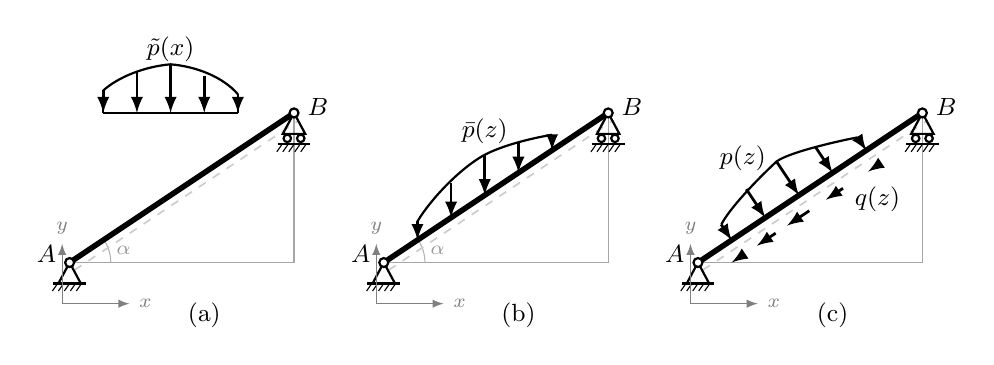
\begin{tikzpicture}[
		scale=0.95,
		>=latex,
		axis/.style={->, thin, gray},
		trave/.style={line width=2pt},
		carico/.style={line width=1pt}, trattcarico/.style={line width=1pt}, 
		pcomp/.style={line width=1pt},
		qcomp/.style={line width=1pt},
		tratt/.style={gray!70, thin}, 
		fibre/.style={dashed, gray!40, line width=0.6pt},
		]
		]
		
		% ── Parametri dei vincoli (convenzione C06/C07) ──
		\def\tw{0.15}    % semi-larghezza triangolo
		\def\thR{0.28}   % altezza triangolo
		\def\rn{0.06}    % raggio anellino (perno)
		\def\rw{0.05}    % raggio ruote del carrello
		\def\bw{0.09}    % semi-distanza ruote
		\def\gw{0.22}    % semi-larghezza barra di terra
		\def\hh{0.10}    % profondità del tratteggio del suolo
		
		
		% =========================================================
		% PANNELLO (a)
		% =========================================================
		\begin{scope}[xshift=0cm]
			
			\draw[trattcarico] (0.45,2) -- (2.25,2);
			%\draw[tratt] (0,0) -- (2,0);
			\draw[tratt] (0,0) -- (3,0);
			\draw[tratt] (3,0) -- (3,2);
			
			
			\draw[gray!60] (0.55,0) arc (0:33.7:0.55);
			\node[gray!80, font=\scriptsize] at (0.72,0.16) {$\alpha$};
			
			\draw[trave] (0,0) -- (3,2);
			\draw[fibre] (0.0666,-0.0998) -- (3.0666,1.9002);
			
			% ── Cerniera in A=(0,0) (suolo orizzontale) ──
			\draw[thick] (0,0) -- (-\tw,-\thR) -- (\tw,-\thR) -- cycle;
			\draw[thick] (-\gw,-\thR) -- (\gw,-\thR);
			\foreach \x in {-0.16,-0.08,0,0.08,0.16}
			\draw[thin] (\x,-\thR) -- ++(-0.07,-\hh);
			
			% ── Carrello in B=(3,2), asse di scorrimento orizzontale ──
			\draw[thick] (3,2) -- (3-\tw,2-\thR) -- (3+\tw,2-\thR) -- cycle;
			\draw[thick] (3-\bw,2-\thR-\rw-0.01) circle (\rw);
			\draw[thick] (3+\bw,2-\thR-\rw-0.01) circle (\rw);
			\draw[thick] (3-\gw,2-\thR-2*\rw-0.04) -- (3+\gw,2-\thR-2*\rw-0.04);
			\foreach \x in {-0.16,-0.08,0,0.08,0.16}
			\draw[thin] (3+\x,2-\thR-2*\rw-0.04) -- ++(-0.07,-\hh);
			
			% ── Anellini (perni) in A e B ──
			\draw[thick, fill=white] (0,0) circle (\rn);
			\draw[thick, fill=white] (3,2) circle (\rn);
			
			% ── Etichette A e B ──
			\node[left,  font=\small] at (-0.05, 0.12) {$A$};
			\node[right, font=\small] at ( 3.05, 2.08) {$B$};
			
			% Frecce: coda sulla curva (sopra y=2), punta su y=2
			\foreach \t/\h in {0.15/0.30, 0.30/0.55, 0.45/0.65,
				0.60/0.50, 0.75/0.25}{
				\pgfmathsetmacro{\px}{3*\t}
				\draw[->, carico] (\px, 2+\h) -- (\px, 2);
			}
			
			% Curva liscia sopra y=2
			\draw[carico, line width=0.8pt]	(0.45, 2.30)
			.. controls (0.65, 2.48) and (1.00, 2.62) ..
			(1.35, 2.65)
			.. controls (1.70, 2.62) and (2.05, 2.48) ..
			(2.25, 2.25);
			
			\draw[carico, line width=0.6pt] (0.45,2.30) -- (0.45,2);
			\draw[carico, line width=0.6pt] (2.25,2.25) -- (2.25,2);
			
			% Label sopra la curva, centrata
			\node[font=\small] at (1.35,2.85){$\tilde{p}(x)$};
			
			\draw[axis] (-0.1,-0.55) -- (0.8,-0.55)
			node[right, font=\scriptsize] {$x$};
			\draw[axis] (-0.1,-0.55) -- (-0.1,0.25)
			node[above, font=\scriptsize] {$y$};
			
			\node[font=\small] at (1.8,-0.70) {(a)};
			
		\end{scope}
		
		% =========================================================
		% PANNELLO (b)
		% =========================================================
		\begin{scope}[xshift=4.2cm]
			
			\draw[tratt] (0,0) -- (3,0);
			\draw[tratt] (3,0) -- (3,2);
			
			\draw[gray!60] (0.55,0) arc (0:33.7:0.55);
			\node[gray!80, font=\scriptsize] at (0.72,0.16) {$\alpha$};
			
			\draw[trave] (0,0) -- (3,2);
			\draw[fibre] (0.0666,-0.0998) -- (3.0666,1.9002);
			
			% ── Cerniera in A=(0,0) ──
			\draw[thick] (0,0) -- (-\tw,-\thR) -- (\tw,-\thR) -- cycle;
			\draw[thick] (-\gw,-\thR) -- (\gw,-\thR);
			\foreach \x in {-0.16,-0.08,0,0.08,0.16}
			\draw[thin] (\x,-\thR) -- ++(-0.07,-\hh);
			
			% ── Carrello in B=(3,2), asse di scorrimento orizzontale ──
			\draw[thick] (3,2) -- (3-\tw,2-\thR) -- (3+\tw,2-\thR) -- cycle;
			\draw[thick] (3-\bw,2-\thR-\rw-0.01) circle (\rw);
			\draw[thick] (3+\bw,2-\thR-\rw-0.01) circle (\rw);
			\draw[thick] (3-\gw,2-\thR-2*\rw-0.04) -- (3+\gw,2-\thR-2*\rw-0.04);
			\foreach \x in {-0.16,-0.08,0,0.08,0.16}
			\draw[thin] (3+\x,2-\thR-2*\rw-0.04) -- ++(-0.07,-\hh);
			
			% ── Anellini in A e B ──
			\draw[thick, fill=white] (0,0) circle (\rn);
			\draw[thick, fill=white] (3,2) circle (\rn);
			
			% ── Etichette A e B ──
			\node[left,  font=\small] at (-0.05, 0.12) {$A$};
			\node[right, font=\small] at ( 3.05, 2.08) {$B$};
			
			% Frecce: coda sulla curva (sopra trave), punta sulla trave
			\foreach \t/\h in {0.15/0.30, 0.30/0.55, 0.45/0.65,
				0.60/0.50, 0.75/0.25}{
				\pgfmathsetmacro{\px}{3*\t}
				\pgfmathsetmacro{\py}{2*\t}
				\pgfmathsetmacro{\hb}{\h*0.8321}
				\draw[->, carico] (\px, \py+\hb) -- (\px, \py);
			}
			
			% Curva liscia (code):
			\draw[carico, line width=0.8pt]
			(0.45, 0.550)
			.. controls (0.65, 0.88) and (1.05, 1.28) ..
			(1.35, 1.441)
			.. controls (1.62, 1.58) and (2.02, 1.67) ..
			(2.25, 1.708);
			
			\draw[carico, line width=0.6pt] (0.45,0.550) -- (0.45,0.30);
			\draw[carico, line width=0.6pt] (2.25,1.708) -- (2.25,1.50);
			
			% Label sopra la curva
			\node[font=\small] at (1.35,1.75){$\bar{p}(z)$};
			
			\draw[axis] (-0.1,-0.55) -- (0.8,-0.55)
			node[right, font=\scriptsize] {$x$};
			\draw[axis] (-0.1,-0.55) -- (-0.1,0.25)
			node[above, font=\scriptsize] {$y$};
			
			\node[font=\small] at (1.8,-0.70) {(b)};
			
		\end{scope}
		
		% =========================================================
		% PANNELLO (c)
		% =========================================================
		\begin{scope}[xshift=8.4cm]
			
			\draw[trave] (0,0) -- (3,2);
			\draw[fibre] (0.0666,-0.0998) -- (3.0666,1.9002);
			\draw[tratt] (0,0) -- (3,0);
			\draw[tratt] (3,0) -- (3,2);
			
			% ── Cerniera in A=(0,0) ──
			\draw[thick] (0,0) -- (-\tw,-\thR) -- (\tw,-\thR) -- cycle;
			\draw[thick] (-\gw,-\thR) -- (\gw,-\thR);
			\foreach \x in {-0.16,-0.08,0,0.08,0.16}
			\draw[thin] (\x,-\thR) -- ++(-0.07,-\hh);
			
			% ── Carrello in B=(3,2), asse di scorrimento orizzontale ──
			\draw[thick] (3,2) -- (3-\tw,2-\thR) -- (3+\tw,2-\thR) -- cycle;
			\draw[thick] (3-\bw,2-\thR-\rw-0.01) circle (\rw);
			\draw[thick] (3+\bw,2-\thR-\rw-0.01) circle (\rw);
			\draw[thick] (3-\gw,2-\thR-2*\rw-0.04) -- (3+\gw,2-\thR-2*\rw-0.04);
			\foreach \x in {-0.16,-0.08,0,0.08,0.16}
			\draw[thin] (3+\x,2-\thR-2*\rw-0.04) -- ++(-0.07,-\hh);
			
			% ── Anellini in A e B ──
			\draw[thick, fill=white] (0,0) circle (\rn);
			\draw[thick, fill=white] (3,2) circle (\rn);
			
			% ── Etichette A e B ──
			\node[left,  font=\small] at (-0.05, 0.12) {$A$};
			\node[right, font=\small] at ( 3.05, 2.08) {$B$};
			
			% ----- p(z): frecce perp alla trave, lato superiore -----
			\foreach \t/\h in {0.15/0.30, 0.30/0.55, 0.45/0.65,
				0.60/0.50, 0.75/0.25}{
				\pgfmathsetmacro{\px}{3*\t}
				\pgfmathsetmacro{\py}{2*\t}
				\pgfmathsetmacro{\hb}{\h*0.8321}
				\pgfmathsetmacro{\cx}{\px - \hb*0.5547}
				\pgfmathsetmacro{\cy}{\py + \hb*0.8321}
				\draw[->, pcomp] (\cx,\cy) -- (\px,\py);
			}
			
			% Curva liscia p(z)
			\draw[pcomp, line width=0.8pt]
			(0.312, 0.508)
			.. controls (0.42, 0.72) and (0.78, 1.10) ..
			(1.050, 1.350)
			.. controls (1.22, 1.48) and (1.95, 1.64) ..
			(2.135, 1.673);
			
			% Chiusura ai bordi
			\draw[pcomp, line width=0.6pt] (0.312,0.508) -- (0.45,0.30);
			\draw[pcomp, line width=0.6pt] (2.135,1.673) -- (2.25,1.50);
			
			% Label p(z)
			\node[font=\small] at (0.60,1.40){$p(z)$};
			
			% ----- q(z): frecce parallele, lato inferiore, verso A -----
			\def\doff{0.25}
			\foreach \t/\h in {0.15/0.30, 0.30/0.55, 0.45/0.65,
				0.60/0.50, 0.75/0.25}{
				\pgfmathsetmacro{\px}{3*\t}
				\pgfmathsetmacro{\py}{2*\t}
				\pgfmathsetmacro{\ox}{\px + \doff*0.5547}
				\pgfmathsetmacro{\oy}{\py - \doff*0.8321}
				\pgfmathsetmacro{\ql}{\h*0.55}
				\pgfmathsetmacro{\ex}{\ox - \ql*0.8321}
				\pgfmathsetmacro{\ey}{\oy - \ql*0.5547}
				\draw[->, qcomp] (\ox,\oy) -- (\ex,\ey);
			}
			
			% Label q(z)
			\node[font=\small] at (2.40,0.85)	{$q(z)$};
			
			\draw[axis] (-0.1,-0.55) -- (0.8,-0.55)
			node[right, font=\scriptsize] {$x$};
			\draw[axis] (-0.1,-0.55) -- (-0.1,0.25)
			node[above, font=\scriptsize] {$y$};
			
			\node[font=\small] at (1.8,-0.70) {(c)};
			
		\end{scope}
		
	\end{tikzpicture}
	\caption{Trave inclinata di $\alpha$ soggetta a carico verticale
		$\tilde{p}(x)$ per unità di proiezione orizzontale.
		(a)~carico $\tilde{p}(x)$: frecce verticali con punte
		sulla retta orizzontale passante per $B$ e code sulla curva;
		(b)~carico equivalente $\bar{p}(z) = \tilde{p}\cos\alpha$
		per unità di lunghezza d'asse: frecce verticali con punte
		sulla trave e code sulla curva;
		(c)~scomposizione negli assi intrinseci:
		$p(z) = \bar{p}\cos\alpha$ (frecce perpendicolari alla trave,
		lato superiore) e $q(z) = \bar{p}\sin\alpha$
		(frecce parallele alla trave, lato inferiore,
		discordi con $z^e$).}
	\label{fig:stat_misto_carico_inclinato}
\end{figure}


Il procedimento si articola in due passi,
illustrati nella
\FIGref{fig:stat_misto_carico_inclinato}.
Nel primo passo si impone l'equivalenza tra
il carico assegnato in proiezione e quello
per unità di lunghezza d'asse: per un carico
verticale $\tilde{p}(x)$ diretto verso il
basso (verso $-y$) per unità di $x$
(\FIGref{fig:stat_misto_carico_inclinato}\,a),
poiché $\dd x = \cos\alpha\,\dd z$, si ha
$\tilde{p}(x)\,\dd x = \bar{p}(z)\,\dd z$ e quindi:
\[
\bar{p}(z) = \tilde{p}(x)\cos\alpha.
\]
Il carico $\bar{p}(z)$ è ancora diretto verso
il basso, di intensità ridotta del fattore
$\cos\alpha$
(\FIGref{fig:stat_misto_carico_inclinato}\,b).
Nel secondo passo si scompone $\bar{p}(z)$
nelle componenti intrinseche
(\FIGref{fig:stat_misto_carico_inclinato}\,c):
\begin{equation}
	p(z) = \bar{p}(z)\cos\alpha= \tilde{p}(z)\cos^2\alpha, \quad
	q(z) = \bar{p}(z)\sin\alpha= \tilde{p}(z)\sin\alpha\cos\alpha.
\end{equation}
La componente $p(z)$ è diretta verso le fibre
inferiori (concorde con $+y^e$); la componente
$q(z)$ è diretta verso $A$ (discorde con
$+z^e$), come mostrato in
\FIGref{fig:stat_misto_carico_inclinato}\,c.

Poiché $x = z\cos\alpha$ e $y = z\sin\alpha$,
il passaggio dalla proiezione al riferimento
intrinseco introduce solo un fattore geometrico
costante che scala l'intensità ma non altera
il grado polinomiale in $z$: un carico
uniforme resta uniforme, un carico lineare
resta lineare, e così via. Le proprietà
qualitative dei diagrammi $N$, $T$, $M$ si
conservano quindi nel passaggio dalla
proiezione al riferimento intrinseco.




\begin{esempio}[Trave con carrello inclinato e forza concentrata]
	Si consideri una trave piana di lunghezza $\ell$
	con cerniera in $A$ e carrello in $B$ con piano
	di scorrimento inclinato di $\pi/4$ in senso
	antiorario rispetto all'orizzontale, soggetta
	a una forza concentrata verticale $Y(C) = P$
	(verso il basso) applicata in mezzeria $C$
	$(z = \ell/2)$ (\FIGref{fig:stat_misto_iso_01}\,a).
	Si costruiscano i diagrammi di $N(z)$, $T(z)$
	e $M(z)$.
	
	\begin{svolgimento}
		
		\begin{figure}[htbp]
			\centering
			\begin{tikzpicture}[scale=0.95,>=latex,
				trave/.style={line width=1.2pt},
				forza/.style={black, line width=1pt},
				quota/.style={black, line width=0.4pt},
				diagN/.style={black, line width=0.8pt},
				diagT/.style={black, line width=0.8pt},
				diagM/.style={black, line width=0.8pt},
				hatch/.style={gray!40, line width=0.3pt},
				]
				% ── Parametri vincoli (convenzione C06/C07) ──
				\def\tw{0.15}\def\thR{0.28}\def\rn{0.06}
				\def\rw{0.05}\def\bw{0.09}\def\gw{0.22}\def\hh{0.10}
				\def\Lb{4}        % lunghezza trave (unità di disegno)
				\def\hT{0.5}      % altezza visiva di P/2 (diagrammi N, T)
				\def\hM{0.8}      % profondità visiva di Pl/4 (diagramma M)
				% ── trave + cerniera A + carrello inclinato B + perni + etichette ──
				\def\supporti{%
					\draw[trave] (0,0) -- (\Lb,0);
					\draw[thick] (0,0) -- (-\tw,-\thR) -- (\tw,-\thR) -- cycle;
					\draw[thick] (-\gw,-\thR) -- (\gw,-\thR);
					\foreach \x in {-0.16,-0.08,0,0.08,0.16}
					\draw[thin] (\x,-\thR) -- ++(-0.07,-\hh);
					\begin{scope}[shift={(\Lb,0)}, rotate=45]
						\draw[thick] (0,0) -- (-\tw,-\thR) -- (\tw,-\thR) -- cycle;
						\draw[thick] (-\bw,-\thR-\rw-0.01) circle (\rw);
						\draw[thick] (\bw,-\thR-\rw-0.01) circle (\rw);
						\draw[thick] (-\gw,-\thR-2*\rw-0.04) -- (\gw,-\thR-2*\rw-0.04);
						\foreach \x in {-0.16,-0.08,0,0.08,0.16}
						\draw[thin] (\x,-\thR-2*\rw-0.04) -- ++(-0.07,-\hh);
					\end{scope}
					\draw[thick, fill=white] (0,0) circle (\rn);
					\draw[thick, fill=white] (\Lb,0) circle (\rn);
					\node[above left=-2pt, font=\small] at (0,0) {$A$};
					\node[above, font=\small] at (\Lb,0) {$B$};}
				
				% ========================= (a) schema =========================
				\begin{scope}[xshift=0cm, yshift=0cm]
					\supporti
					\draw[thin, gray!60] (\Lb,0) -- ++(0:0.95);   % prolungamento asse trave (riferimento orizzontale)
					\draw[thin, gray!60] (\Lb,0) -- ++(45:0.95);  % direzione del piano di scorrimento
					\draw[gray!60] (\Lb+0.62,0) arc (0:45:0.62);
					\node[gray!80, font=\scriptsize] at (\Lb+0.86,0.30) {$\pi/4$};
					\draw[->, forza] (\Lb/2, 0.95) -- (\Lb/2, 0.03);
					\node[right, font=\small] at (\Lb/2+0.04, 0.58) {$P$};
					\node[below, font=\footnotesize] at (\Lb/2,-0.02) {$C$};
					\def\yq{-0.80}
					\draw[quota, <->] (0,\yq) -- (\Lb/2,\yq);
					\draw[quota] (0,\yq+0.10) -- (0,\yq-0.10);
					\draw[quota] (\Lb/2,\yq+0.10) -- (\Lb/2,\yq-0.10);
					\node[above, font=\footnotesize] at (\Lb/4,\yq) {$\ell/2$};
					\node[font=\small] at (2*\Lb/3,-1.0) {(a)};
				\end{scope}
				
				% ============ (b) N: uniforme in compressione, sotto l'asse ============
				\begin{scope}[xshift=6.8cm, yshift=0cm]
					\foreach \x in {0.10,0.30,...,3.90}\draw[hatch] (\x,0)--(\x,-\hT);
					\draw[diagN] (0,0)--(0,-\hT)--(\Lb,-\hT)--(\Lb,0);
					\node[font=\small] at (\Lb/2,-0.5*\hT) {$\boldsymbol{\ominus}$};
					\node[left, font=\small] at (0,-\hT-0.2) {$\tfrac{P}{2}$};
					\supporti
					\node[font=\small] at (2*\Lb/3,-1.0) {(b)};
				\end{scope}
				
				% ========== (c) T: +P/2 sopra (AC), -P/2 sotto (CB) ==========
				\begin{scope}[xshift=0cm, yshift=-2.25cm]
					\foreach \x in {0.10,0.30,...,1.90}\draw[hatch] (\x,0)--(\x,\hT);
					\foreach \x in {2.10,2.30,...,3.90}\draw[hatch] (\x,0)--(\x,-\hT);
					\draw[diagT] (0,0)--(0,\hT)--(\Lb/2,\hT)--(\Lb/2,-\hT)--(\Lb,-\hT)--(\Lb,0);
					\node[font=\small] at (\Lb/4,0.5*\hT) {$\boldsymbol{\oplus}$};
					\node[font=\small] at (3*\Lb/4,-0.5*\hT) {$\boldsymbol{\ominus}$};
					\node[right, font=\small] at (\Lb/2,\hT) {$\tfrac{P}{2}$};
					\node[left, font=\small] at (\Lb/2,-\hT) {$\tfrac{P}{2}$};
					\supporti
					\node[font=\small] at (2*\Lb/3,-1.0) {(c)};
				\end{scope}
				
				% ============= (d) M: triangolo sotto, max in C =============
				\begin{scope}[xshift=6.8cm, yshift=-2.25cm]
					\foreach \x in {0.20,0.40,...,1.80}{%
						\pgfmathsetmacro{\h}{-\hM*\x/(\Lb/2)}\draw[hatch] (\x,0)--(\x,\h);}
					\foreach \x in {2.20,2.40,...,3.80}{%
						\pgfmathsetmacro{\h}{-\hM*(\Lb-\x)/(\Lb/2)}\draw[hatch] (\x,0)--(\x,\h);}
					\draw[diagM] (0,0)--(\Lb/2,-\hM)--(\Lb,0);
					\node[above, font=\small] at (\Lb/2,-\hM-0.02) {$\tfrac{P\ell}{4}$};
					\supporti
					\node[font=\small] at (2*\Lb/3,-1.0) {(d)};
				\end{scope}
				
			\end{tikzpicture}
			\caption{Trave con cerniera in $A$ e carrello inclinato di $\pi/4$
				in $B$, con forza concentrata $P$ in mezzeria $C$:
				(a)~schema strutturale; (b)~sforzo normale $N$, uniforme in
				compressione $-P/2$; (c)~taglio $T$, pari a $+P/2$ nel tratto
				$AC$ e $-P/2$ nel tratto $CB$, con salto $-P$ in $C$;
				(d)~momento flettente $M$, lineare a tratti con massimo
				$P\ell/4$ in $C$.}
			\label{fig:stat_misto_iso_01}
		\end{figure}
		

		\esottotit{Reazioni vincolari.}
		Il carrello in $B$ ha piano di scorrimento
		inclinato di $\pi/4$: la sua reazione è
		perpendicolare al piano di scorrimento,
		quindi inclinata di $3\pi/4$ rispetto
		all'orizzontale. Le componenti orizzontale
		e verticale della reazione in $B$ sono
		uguali in modulo e legate da:
		\[
		H_B = -V_B
		\quad\text{(componente orizzontale verso
			sinistra se $V_B$ verso l'alto)}.
		\]
		Questo accoppiamento rende il problema misto:
		le reazioni longitudinali e trasversali non
		sono indipendenti.
		Si assumono $H_A$ positivo verso destra,
		$V_A$ e $V_B$ positivi verso l'alto.
		Dall'equilibrio globale:
		\[
		\sum \mu_A = 0:\quad
		V_B\ell - P\cdot\frac{\ell}{2} = 0
		\;\Rightarrow\;
		V_B = \frac{P}{2},
		\]
		\[
		\sum V = 0:\quad
		V_A + V_B - P = 0
		\;\Rightarrow\;
		V_A = \frac{P}{2},
		\]
		\[
		\sum H = 0:\quad
		H_A + H_B = 0
		\;\Rightarrow\;
		H_A = -H_B = V_B = \frac{P}{2}
		\quad\text{(verso destra)}.
		\]
		
		\esottotit{Condizioni al contorno.}
		All'estremo $A$ (cerniera): $H_A$ è verso
		destra (concorde con $+z^e$) e $V_A$ è verso
		l'alto (discorde con $+y^e$); pertanto:
		\[
		N(A) = -H_A = -\frac{P}{2}
		\quad\text{(compressione)},
		\qquad
		T(A) = V_A = \frac{P}{2},
		\qquad
		M(A) = 0.
		\]
		All'estremo $B$ (carrello): $H_B$ è verso
		sinistra (discorde con $+z^e$) e $V_B$ è verso
		l'alto (discorde con $+y^e$); pertanto:
		\[
		N(B) = H_B = -\frac{P}{2}
		\quad\text{(compressione)},
		\qquad
		T(B) = -V_B = -\frac{P}{2},
		\qquad
		M(B) = 0.
		\]
		
		\esottotit{Analisi qualitativa.}
		\begin{itemize}[nosep]
			\item su tutta la trave: $q = 0$, quindi
			$N' = 0$ e $N$ è \emph{uniforme};
			\item nei tratti $AC$ e $CB$: $p = 0$,
			quindi $T' = 0$ e $T$ è
			\emph{uniforme} in ciascun tratto;
			\item in $C$: forza $Y(C) = P$ verso il
			basso, quindi $T$ presenta un
			\emph{salto negativo} $-P$; $N$ e
			$M$ sono \emph{continui};
			\item nei tratti $AC$ e $CB$: $c = 0$ e
			$T$ uniforme, quindi $M$ è
			\emph{lineare} in ciascun tratto;
			$T > 0$ in $AC$ e $T < 0$ in $CB$,
			quindi $M$ è crescente in $AC$ e
			decrescente in $CB$, con massimo
			in $C$.
		\end{itemize}
		
		\esottotit{Diagramma dello sforzo normale.}
		
		Su tutta la trave, guardando a sinistra,
		$\mathcal{C}^-(z)$ contiene $H_A$ (verso
		destra, concorde con $+z^e$):
		\[
		N(z) = -H_A = -\frac{P}{2}.
		\]
		Uniforme in compressione su tutta la trave,
		in accordo con l'analisi qualitativa.
		
		\esottotit{Diagramma del taglio.}
		
		\textit{Tratto $AC$ $(0 \leq z \leq \ell/2)$:}
		Guardando a sinistra, $\mathcal{C}^-(z)$
		contiene la sola reazione $V_A$:
		\[
		T(z) = V_A = \frac{P}{2}.
		\]
		
		\textit{Tratto $CB$ $(\ell/2 < z \leq \ell)$:}
		Guardando a destra, $\mathcal{C}^+(z)$
		contiene la sola reazione $V_B$ (verso l'alto,
		discorde con $+y^e$):
		\[
		T(z) = -V_B = -\frac{P}{2}.
		\]
		
		\esottotit{Verifica del salto in $C$:}
		\[
		T((\ell/2)^+) - T((\ell/2)^-)
		= -\frac{P}{2} - \frac{P}{2}
		= -P = -Y(C). \quad\checkmark
		\]
		
		\esottotit{Diagramma del momento flettente.}
		
		\textit{Tratto $AC$ $(0 \leq z \leq \ell/2)$:}
		Guardando a sinistra, $\mathcal{C}^-(z)$
		contiene $V_A$ e $H_A$; poiché $H_A$ è
		longitudinale non contribuisce a $M$:
		\[
		M(z) = V_A z = \frac{P}{2}z.
		\]
		Lineare crescente da $M(0) = 0$ a
		$M(\ell/2) = P\ell/4$.
		
		\textit{Tratto $CB$ $(\ell/2 < z \leq \ell)$:}
		Guardando a destra, $\mathcal{C}^+(z)$
		contiene $V_B$ (verso l'alto, a distanza
		$\ell - z$) e $H_B$; poiché $H_B$ è
		longitudinale non contribuisce a $M$:
		\[
		M(z) = V_B(\ell - z) = \frac{P}{2}(\ell - z).
		\]
		Lineare decrescente da $M(\ell/2) = P\ell/4$
		a $M(\ell) = 0$.
		
		\esottotit{Lettura per aree.}
		Le variazioni di $M$ nei due tratti si leggono
		come aree dei rettangoli sottesi da $T$:
		\[
		\Delta M_{AC} = \frac{P}{2}\cdot\frac{\ell}{2}
		= \frac{P\ell}{4}, \quad
		\Delta M_{CB} = -\frac{P}{2}\cdot\frac{\ell}{2}
		= -\frac{P\ell}{4}.
		\]
		Somma totale nulla, confermando
		$M(\ell) = 0$. $\quad\checkmark$
		
		\noindent
		Nel problema misto tutti e tre i diagrammi
		$N(z)$, $T(z)$, $M(z)$ sono non banali: il
		carrello inclinato introduce reazioni con
		componenti sia longitudinali che trasversali,
		rendendo non nulle le condizioni al contorno
		per tutte e tre le caratteristiche della
		sollecitazione, e generando uno sforzo normale
		uniforme in compressione $N = -P/2$ anche
		in assenza di carichi longitudinali
		(\FIGref{fig:stat_misto_iso_01}\,b).
		Il diagramma di $T(z)$ è uniforme a tratti:
		$+P/2$ nel tratto $AC$ e $-P/2$ nel tratto
		$CB$, con salto negativo $-P$ in $C$
		(\FIGref{fig:stat_misto_iso_01}\,c).
		Il diagramma di $M(z)$ è lineare a tratti
		con massimo $P\ell/4$ in $C$ e nullo agli
		estremi (\FIGref{fig:stat_misto_iso_01}\,d).
	\end{svolgimento}
\end{esempio}


\begin{esempio}[Trave inclinata con carico verticale uniforme]
	Si consideri una trave piana inclinata di
	$\alpha = \pi/4$ rispetto all'orizzontale,
	con cerniera in $A$ e carrello verticale in
	$B$, soggetta a un carico verticale
	$\tilde{p}(x) = \tilde{p}_0$ uniforme per unità
	di proiezione orizzontale. La lunghezza della
	proiezione orizzontale è $L$, quindi la
	lunghezza d'asse è $\ell = L\sqrt{2}$.
	Si costruiscano i diagrammi di $N(z)$,
	$T(z)$ e $M(z)$.
	
	\begin{svolgimento}
		
		
		
		\esottotit{Carichi nel riferimento intrinseco.}
		Con $\alpha = \pi/4$ si ha $\cos\alpha =
		\sin\alpha = 1/\sqrt{2}$, quindi
		(\FIGref{fig:stat_misto_inclinata_carichi}):
		\[
		\bar{p}(z) = \tilde{p}_0\cos\alpha
		= \frac{\tilde{p}_0}{\sqrt{2}},
		\qquad
		p(z) = \tilde{p}_0\cos^2\alpha = \frac{\tilde{p}_0}{2},
		\qquad
		q(z) = \frac{\tilde{p}_0}{2}\sin 2\alpha
		= \frac{\tilde{p}_0}{2}.
		\]
		Entrambe le componenti sono uniformi e di
		uguale intensità $\tilde{p}_0/2$: $p(z)$ concorde
		con $+y^e$ (verso le fibre inferiori), $q(z)$
		discorde con $+z^e$ (verso $A$).
		
		\esottotit{Reazioni vincolari.}
		La cerniera in $A$ fornisce $H_A$ e $V_A$;
		il carrello verticale in $B$ fornisce $V_B$.
		Poiché il carico totale equivale a $\tilde{p}_0$
		verticale su proiezione $L$, la risultante
		è $\tilde{p}_0L$ verso il basso applicata in
		mezzeria ($x = L/2$).
		Dall'equilibrio globale:
		\[
		\sum \mu_A = 0:\quad
		V_B L - \tilde{p}_0L\cdot\frac{L}{2} = 0
		\;\Rightarrow\;
		V_B = \frac{\tilde{p}_0L}{2},
		\]
		\[
		\sum V = 0:\quad
		V_A + V_B - \tilde{p}_0L = 0
		\;\Rightarrow\;
		V_A = \frac{\tilde{p}_0L}{2},
		\]
		\[
		\sum H = 0:\quad
		H_A = 0.
		\]
		Le reazioni verticali sono uguali per
		simmetria del carico; la reazione orizzontale
		è nulla perché il carrello verticale non
		fornisce reazione orizzontale e il carico
		è puramente verticale.
		
		\esottotit{Condizioni al contorno.}
		Proiettando le reazioni sugli assi intrinseci
		(con $\cos\alpha = \sin\alpha = 1/\sqrt{2}$):
		
		All'estremo $A$:
		\[
		N(A) = -\frac{V_A}{\sqrt{2}}
		= -\frac{\tilde{p}_0L\sqrt{2}}{4}
		\quad\text{(compressione)},
		\qquad
		T(A) = \frac{V_A}{\sqrt{2}}
		= \frac{\tilde{p}_0L\sqrt{2}}{4},
		\qquad
		M(A) = 0.
		\]
		All'estremo $B$:
		\[
		N(B) = \frac{V_B}{\sqrt{2}}
		= \frac{\tilde{p}_0L\sqrt{2}}{4}
		\quad\text{(trazione)},
		\qquad
		T(B) = -\frac{V_B}{\sqrt{2}}
		= -\frac{\tilde{p}_0L\sqrt{2}}{4},
		\qquad
		M(B) = 0.
		\]
		
		\begin{figure}[htbp]
			\centering
			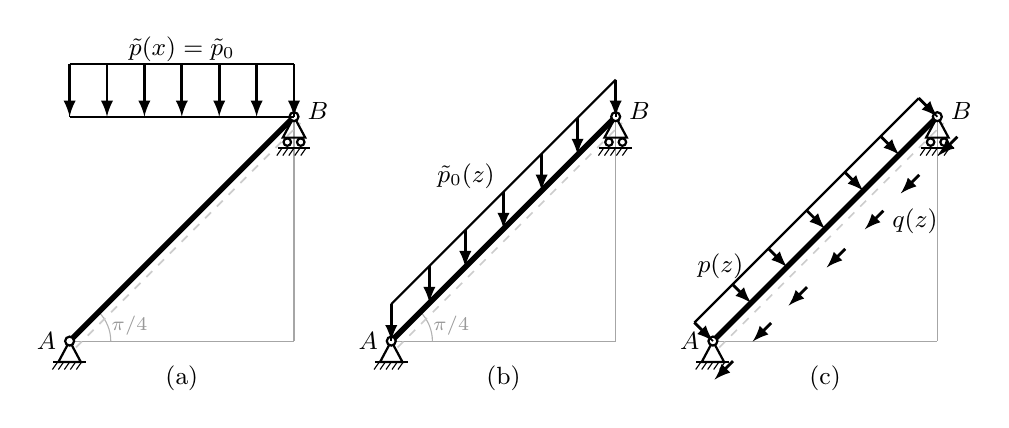
\begin{tikzpicture}[
				scale=0.95,
				>=latex,
				trave/.style={line width=2pt},
				%carico/.style={blue!70!black, line width=1pt},
				carico/.style={line width=1pt},
				%			pcomp/.style={teal!60!black, line width=1pt},
				pcomp/.style={line width=1pt},
				%			qcomp/.style={orange!80!black, line width=1pt},
				qcomp/.style={line width=1pt},
				tratt/.style={gray!70, thin},
				fibre/.style={dashed, gray!40, line width=0.6pt},
				]
				
				% =========================================================
				% PANNELLO (a)
				% =========================================================
				\begin{scope}[xshift=0cm]
					
					% ── Parametri dei vincoli (convenzione C06/C07) ──
					\def\tw{0.15}    % semi-larghezza triangolo
					\def\thR{0.28}   % altezza triangolo
					\def\rn{0.06}    % raggio anellino (perno)
					\def\rw{0.05}    % raggio ruote del carrello
					\def\bw{0.09}    % semi-distanza ruote
					\def\gw{0.22}    % semi-larghezza barra di terra
					\def\hh{0.10}    % profondità del tratteggio del suolo
					
					% ── Linee guida e angolo π/4 ──
					\draw[tratt] (0,0) -- (3,0);
					\draw[tratt] (3,0) -- (3,3);
					
					\draw[gray!60] (0.55,0) arc (0:45:0.55);
					\node[gray!80, font=\scriptsize] at (0.80,0.20) {$\pi/4$};
					
					% ── Trave (con fibra inferiore) ──
					\draw[fibre] (0.0849,-0.0849) -- (3.0849,2.9151);
					\draw[trave] (0,0) -- (3,3);
					
					% ── Cerniera in A=(0,0) (suolo orizzontale) ──
					\draw[thick] (0,0) -- (-\tw,-\thR) -- (\tw,-\thR) -- cycle;
					% barra di terra (alla base del triangolo)
					\draw[thick] (-\gw,-\thR) -- (\gw,-\thR);
					% tratteggio del suolo
					\foreach \x in {-0.16,-0.08,0,0.08,0.16}
					\draw[thin] (\x,-\thR) -- ++(-0.07,-\hh);
					
					% ── Carrello in B=(3,3), asse di scorrimento orizzontale ──
					\draw[thick] (3,3) -- (3-\tw,3-\thR) -- (3+\tw,3-\thR) -- cycle;
					% due ruote (sotto la base del triangolo, tangenti)
					\draw[thick] (3-\bw,3-\thR-\rw-0.01) circle (\rw);
					\draw[thick] (3+\bw,3-\thR-\rw-0.01) circle (\rw);
					% barra di terra (sotto le ruote)
					\draw[thick] (3-\gw,3-\thR-2*\rw-0.04) -- (3+\gw,3-\thR-2*\rw-0.04);
					% tratteggio del suolo
					\foreach \x in {-0.16,-0.08,0,0.08,0.16}
					\draw[thin] (3+\x,3-\thR-2*\rw-0.04) -- ++(-0.07,-\hh);
					
					% ── Anellini (perni) in A e B
					%    disegnati per ultimi per restare in primo piano ──
					\draw[thick, fill=white] (0,0) circle (\rn);
					\draw[thick, fill=white] (3,3) circle (\rn);
					
					% ── Etichette A e B (posizioni originali) ──
					\node[left,  font=\small] at (-0.05, 0.) {$A$};
					\node[right, font=\small] at ( 3.05, 3.08) {$B$};
					
					% ── Carico distribuito p(x) = \tilde{p}_0 ──
					\foreach \px in {0.00, 0.50, 1.00, 1.50, 2.00, 2.50, 3.00}{
						\draw[->, carico] (\px, 3.70) -- (\px, 3);
					}
					\draw[carico, line width=0.8pt]	(0.00, 3.70) -- (3.00, 3.70);
					\draw[carico, line width=0.6pt]	(0.00, 3.70) -- (0.00, 3);
					\draw[carico, line width=0.6pt]	(3.00, 3.70) -- (3.00, 3);
					\draw[carico, line width=0.8pt]	(0.00, 3.0) -- (3.00, 3.0);
					
					\node[font=\small] at (1.50,3.90){$\tilde{p}(x) = \tilde{p}_0$};
					
					% ── Etichetta pannello ──
					\node[font=\small] at (1.5,-0.50) {(a)};
					
				\end{scope}
				
				% =========================================================
				% PANNELLO (b)
				% =========================================================
				\begin{scope}[xshift=4.3cm]
					
					% ── Parametri dei vincoli (convenzione C06/C07) ──
					\def\tw{0.15}    % semi-larghezza triangolo
					\def\thR{0.28}   % altezza triangolo
					\def\rn{0.06}    % raggio anellino (perno)
					\def\rw{0.05}    % raggio ruote del carrello
					\def\bw{0.09}    % semi-distanza ruote
					\def\gw{0.22}    % semi-larghezza barra di terra
					\def\hh{0.10}    % profondità del tratteggio del suolo
					
					% ── Linee guida e angolo π/4 ──
					\draw[tratt] (0,0) -- (3,0);
					\draw[tratt] (3,0) -- (3,3);
					
					\draw[gray!60] (0.55,0) arc (0:45:0.55);
					\node[gray!80, font=\scriptsize] at (0.80,0.20) {$\pi/4$};
					
					% ── Trave (con fibra inferiore) ──
					\draw[fibre] (0.0849,-0.0849) -- (3.0849,2.9151);
					\draw[trave] (0,0) -- (3,3);
					
					% ── Cerniera in A=(0,0) (suolo orizzontale) ──
					\draw[thick] (0,0) -- (-\tw,-\thR) -- (\tw,-\thR) -- cycle;
					% barra di terra (alla base del triangolo)
					\draw[thick] (-\gw,-\thR) -- (\gw,-\thR);
					% tratteggio del suolo
					\foreach \x in {-0.16,-0.08,0,0.08,0.16}
					\draw[thin] (\x,-\thR) -- ++(-0.07,-\hh);
					
					% ── Carrello in B=(3,3), asse di scorrimento orizzontale ──
					% triangolo (outline)
					\draw[thick] (3,3) -- (3-\tw,3-\thR) -- (3+\tw,3-\thR) -- cycle;
					% due ruote (sotto la base del triangolo, tangenti)
					\draw[thick] (3-\bw,3-\thR-\rw-0.01) circle (\rw);
					\draw[thick] (3+\bw,3-\thR-\rw-0.01) circle (\rw);
					% barra di terra (sotto le ruote)
					\draw[thick] (3-\gw,3-\thR-2*\rw-0.04) -- (3+\gw,3-\thR-2*\rw-0.04);
					% tratteggio del suolo
					\foreach \x in {-0.16,-0.08,0,0.08,0.16}
					\draw[thin] (3+\x,3-\thR-2*\rw-0.04) -- ++(-0.07,-\hh);
					
					% ── Anellini (perni) in A e B
					%    disegnati per ultimi per restare in primo piano ──
					\draw[thick, fill=white] (0,0) circle (\rn);
					\draw[thick, fill=white] (3,3) circle (\rn);
					
					% ── Etichette A e B ──
					\node[left,  font=\small] at (-0.05, 0.) {$A$};
					\node[right, font=\small] at ( 3.05, 3.08) {$B$};
					
					% ── Carico distribuito p(z) lungo l'asse della trave ──
					% hb = 0.4950
					\foreach \t in {0.00, 0.17, 0.33, 0.50,
						0.67, 0.83, 1.00}{
						\pgfmathsetmacro{\px}{3*\t}
						\pgfmathsetmacro{\py}{3*\t}
						\draw[->, carico] (\px, \py+0.4950) -- (\px, \py);
					}
					\draw[carico, line width=0.8pt]
					(0.00, 0.4950) -- (3.00, 3.4950);
					\draw[carico, line width=0.6pt]
					(0.00, 0.4950) -- (0.00, 0.00);
					\draw[carico, line width=0.6pt]
					(3.00, 3.4950) -- (3.00, 3.00);
					
					\node[font=\small] at (1.00,2.20){$\tilde{p}_0(z)$};
					
					% ── Etichetta pannello ──
					\node[font=\small] at (1.5,-0.50) {(b)};
					
				\end{scope}
				
				% =========================================================
				% PANNELLO (c)
				% =========================================================
				\begin{scope}[xshift=8.6cm]
					
					% ── Parametri dei vincoli (convenzione C06/C07) ──
					\def\tw{0.15}    % semi-larghezza triangolo
					\def\thR{0.28}   % altezza triangolo
					\def\rn{0.06}    % raggio anellino (perno)
					\def\rw{0.05}    % raggio ruote del carrello
					\def\bw{0.09}    % semi-distanza ruote
					\def\gw{0.22}    % semi-larghezza barra di terra
					\def\hh{0.10}    % profondità del tratteggio del suolo
					
					% ── Linee guida e angolo π/4 ──
					\draw[tratt] (0,0) -- (3,0);
					\draw[tratt] (3,0) -- (3,3);
					
					% ── Trave (con fibra inferiore) ──
					\draw[fibre] (0.0849,-0.0849) -- (3.0849,2.9151);
					\draw[trave] (0,0) -- (3,3);
					
					% ── Cerniera in A=(0,0) (suolo orizzontale) ──
					\draw[thick] (0,0) -- (-\tw,-\thR) -- (\tw,-\thR) -- cycle;
					% barra di terra (alla base del triangolo)
					\draw[thick] (-\gw,-\thR) -- (\gw,-\thR);
					% tratteggio del suolo
					\foreach \x in {-0.16,-0.08,0,0.08,0.16}
					\draw[thin] (\x,-\thR) -- ++(-0.07,-\hh);
					
					% ── Carrello in B=(3,3), asse di scorrimento orizzontale ──
					\draw[thick] (3,3) -- (3-\tw,3-\thR) -- (3+\tw,3-\thR) -- cycle;
					% due ruote (sotto la base del triangolo, tangenti)
					\draw[thick] (3-\bw,3-\thR-\rw-0.01) circle (\rw);
					\draw[thick] (3+\bw,3-\thR-\rw-0.01) circle (\rw);
					% barra di terra (sotto le ruote)
					\draw[thick] (3-\gw,3-\thR-2*\rw-0.04) -- (3+\gw,3-\thR-2*\rw-0.04);
					% tratteggio del suolo
					\foreach \x in {-0.16,-0.08,0,0.08,0.16}
					\draw[thin] (3+\x,3-\thR-2*\rw-0.04) -- ++(-0.07,-\hh);
					
					% ── Anellini (perni) in A e B
					%    disegnati per ultimi per restare in primo piano ──
					\draw[thick, fill=white] (0,0) circle (\rn);
					\draw[thick, fill=white] (3,3) circle (\rn);
					
					% ── Etichette A e B ──
					\node[left,  font=\small] at (-0.05, 0.) {$A$};
					\node[right, font=\small] at ( 3.05, 3.08) {$B$};
					
					% ----- p(z): componente perpendicolare alla trave, lato superiore -----
					\foreach \t in {0.00, 0.17, 0.33, 0.50,
						0.67, 0.83, 1.00}{
						\pgfmathsetmacro{\px}{3*\t}
						\pgfmathsetmacro{\py}{3*\t}
						\pgfmathsetmacro{\cx}{\px - 0.2475}
						\pgfmathsetmacro{\cy}{\py + 0.2475}
						\draw[->, pcomp] (\cx,\cy) -- (\px,\py);
					}
					\draw[pcomp, line width=0.8pt]
					(-0.2475, 0.2475) -- (2.7525, 3.2475);
					\draw[pcomp, line width=0.6pt]
					(-0.2475, 0.2475) -- (0.00, 0.00);
					\draw[pcomp, line width=0.6pt]
					(2.7525, 3.2475) -- (3.00, 3.00);
					
					\node[font=\small] at (0.10,1.00){$p(z)$};
					
					% ----- q(z): componente parallela alla trave, lato inferiore, verso A -----
					\foreach \t in {0.00, 0.17, 0.33, 0.50,
						0.67, 0.83, 1.00}{
						\pgfmathsetmacro{\px}{3*\t}
						\pgfmathsetmacro{\py}{3*\t}
						\pgfmathsetmacro{\ox}{\px + 0.2687}
						\pgfmathsetmacro{\oy}{\py - 0.2687}
						\pgfmathsetmacro{\ex}{\ox - 0.2475}
						\pgfmathsetmacro{\ey}{\oy - 0.2475}
						\draw[->, qcomp] (\ox,\oy) -- (\ex,\ey);
					}
					
					\node[font=\small] at (2.70,1.60)	{$q(z)$};
					
					% ── Etichetta pannello ──
					\node[font=\small] at (1.5,-0.50) {(c)};
					
				\end{scope}
				
			\end{tikzpicture}
			\caption{Trave inclinata di $\pi/4$ con carico
				verticale uniforme $\tilde{p}(x) = \tilde{p}_0$:
				(a)~carico $\tilde{p}(x)$ per unità di
				proiezione orizzontale;
				(b)~carico equivalente $\bar{p}(z) =
				\tilde{p}_0/\sqrt{2}$ per unità di lunghezza d'asse;
				(c)~componenti intrinseche $p(z) = \tilde{p}_0/2$
				(perpendicolare alla trave, lato superiore)
				e $q(z) = \tilde{p}_0/2$ (parallelo alla trave,
				lato inferiore, verso $A$).}
			\label{fig:stat_misto_inclinata_carichi}
		\end{figure}
		
		\esottotit{Analisi qualitativa.}
		\begin{itemize}[nosep]
			\item $q = \tilde{p}_0/2$ uniforme diretto
			verso $A$ (discorde con $+z^e$), quindi
			$N' = -q = +\tilde{p}_0/2$ uniforme e
			$N$ è \emph{lineare crescente}
			da $-\tilde{p}_0L\sqrt{2}/4$ a
			$+\tilde{p}_0L\sqrt{2}/4$: la trave
			è compressa nella prima metà e
			tesa nella seconda, con
			annullamento in mezzeria;
			\item $p = \tilde{p}_0/2$ uniforme, quindi
			$T' = -p = -\tilde{p}_0/2$ uniforme
			e $T$ è \emph{lineare decrescente}
			da $+\tilde{p}_0L\sqrt{2}/4$ a
			$-\tilde{p}_0L\sqrt{2}/4$, con
			annullamento in mezzeria;
			\item $c = 0$ e $T$ lineare, quindi
			$M$ è \emph{parabolico}; poiché
			$M'' = T' = -\tilde{p}_0/2 < 0$,
			il diagramma ha concavità verso
			l'alto; $M(A) = M(B) = 0$ e
			massimo in mezzeria.
		\end{itemize}
		
		\esottotit{Diagramma di $N$.}
		Guardando a sinistra, $\mathcal{C}^-(z)$
		contiene $V_A$ (componente longitudinale
		$+V_A/\sqrt{2}$, concorde con $+z^e$) e il
		carico $q = \tilde{p}_0/2$ diretto verso $A$
		(componente $-qz$ su $[0,z]$, discorde con
		$+z^e$). Per la regola del segno di
		$\mathcal{C}^-$ si ha
		$N(z) = -\bigl(\tfrac{V_A}{\sqrt{2}} - qz\bigr)$;
		quindi:
		\[
		N(z) = -\frac{V_A}{\sqrt{2}} + \frac{\tilde{p}_0}{2}z
		= -\frac{\tilde{p}_0L\sqrt{2}}{4}
		+ \frac{\tilde{p}_0}{2}z
		= \frac{\tilde{p}_0}{2}
		\!\left(z - \frac{L\sqrt{2}}{2}\right).
		\]
		Lineare crescente, nullo in $z = \ell/2$
		(mezzeria), in accordo con l'analisi qualitativa.
		
		\esottotit{Diagramma di $T$.}
		Con $p = \tilde{p}_0/2$ e $T(0) =
		\tilde{p}_0L\sqrt{2}/4$:
		\[
		T(z) = \frac{\tilde{p}_0L\sqrt{2}}{4}
		- \frac{\tilde{p}_0}{2}z
		= \frac{\tilde{p}_0}{2}
		\!\left(\frac{L\sqrt{2}}{2} - z
		\right).
		\]
		Lineare, nullo in mezzeria, in accordo
		con l'analisi qualitativa.
		
		\esottotit{Diagramma di $M$.}
		Il momento flettente si esprime più
		naturalmente nella coordinata di proiezione
		orizzontale $x = z\cos\alpha =
		z/\sqrt{2}$. Guardando a sinistra,
		$\mathcal{C}^-(x)$ contiene $V_A$ e il
		carico verticale $\tilde{p}_0$ su $[0,x]$:
		\[
		M(x) = V_A x - \tilde{p}_0x\cdot\frac{x}{2}
		= \frac{\tilde{p}_0L}{2}x
		- \frac{\tilde{p}_0}{2}x^2
		= \frac{\tilde{p}_0}{2}x(L - x).
		\]
		Parabolico, nullo agli estremi, con massimo
		in $x = L/2$ (mezzeria in proiezione):
		\[
		M\!\left(\frac{L}{2}\right)
		= \frac{\tilde{p}_0L^2}{8}.
		\]
		Il valore massimo è identico a quello della
		trave orizzontale appoggiata con lo stesso
		carico $\tilde{p}_0$ su lunghezza $L$: il
		momento flettente non risente
		dell'inclinazione della trave.
		
		\begin{figure}[htbp]
			\centering
			\begin{tikzpicture}[
				scale=0.95,
				>=latex,
				trave/.style={line width=2pt},
				diagN/.style={black, line width=0.8pt},
				diagT/.style={black, line width=0.8pt},
				diagM/.style={black, line width=0.8pt},
				fibre/.style={dashed, gray!40, line width=0.6pt},
				]
				
				]
				
				% ── Parametri e macro dei vincoli (convenzione C06/C07) ──
				\def\tw{0.15}\def\thR{0.28}\def\rn{0.06}
				\def\rw{0.05}\def\bw{0.09}\def\gw{0.22}\def\hh{0.10}
				\def\vincoli{%
					% Cerniera in A=(0,0)
					\draw[thick] (0,0) -- (-\tw,-\thR) -- (\tw,-\thR) -- cycle;
					\draw[thick] (-\gw,-\thR) -- (\gw,-\thR);
					\foreach \x in {-0.16,-0.08,0,0.08,0.16}
					\draw[thin] (\x,-\thR) -- ++(-0.07,-\hh);
					% Carrello verticale in B=(3,3)
					\draw[thick] (3,3) -- (3-\tw,3-\thR) -- (3+\tw,3-\thR) -- cycle;
					\draw[thick] (3-\bw,3-\thR-\rw-0.01) circle (\rw);
					\draw[thick] (3+\bw,3-\thR-\rw-0.01) circle (\rw);
					\draw[thick] (3-\gw,3-\thR-2*\rw-0.04) -- (3+\gw,3-\thR-2*\rw-0.04);
					\foreach \x in {-0.16,-0.08,0,0.08,0.16}
					\draw[thin] (3+\x,3-\thR-2*\rw-0.04) -- ++(-0.07,-\hh);
					% Anellini (perni)
					\draw[thick, fill=white] (0,0) circle (\rn);
					\draw[thick, fill=white] (3,3) circle (\rn);
					% Etichette
					\node[left,  font=\small] at (-0.05, 0.12) {$A$};
					\node[right, font=\small] at ( 3.05, 3.08) {$B$};}
				
				% =========================================================
				% PANNELLO (a): N
				% =========================================================
				\begin{scope}[xshift=0cm]
					
					\draw[fibre] (0.0849,-0.0849) -- (3.0849,2.9151);
					\draw[trave] (0,0) -- (3,3);
					
					\vincoli
					
					\draw[diagN, line width=0.8pt]
					(0.6364,-0.6364) -- (0.8091,-0.2091) --
					(0.9818, 0.2182) -- (1.1546, 0.6454) --
					(1.3273, 1.0727) -- (1.5000, 1.5000) --
					(1.6727, 1.9273) -- (1.8454, 2.3546) --
					(2.0182, 2.7818) -- (2.1909, 3.2091) --
					(2.3636, 3.6364);
					
					\draw[diagN, line width=0.6pt]	(0,0) -- (0.6364,-0.6364);
					\draw[diagN, line width=0.6pt]	(3,3) -- (2.3636,3.6364);
					
					% Campiture N — P(t)=(3t,3t), tutti corretti
					% Prima metà f=(1-2t)*0.6364, t=0.05..0.45
					\draw[diagN,line width=0.3pt](0.15, 0.15)--(0.15+0.5728, 0.15-0.5728);
					\draw[diagN,line width=0.3pt](0.30, 0.30)--(0.30+0.5092, 0.30-0.5092);
					\draw[diagN,line width=0.3pt](0.45, 0.45)--(0.45+0.4456, 0.45-0.4456);
					\draw[diagN,line width=0.3pt](0.60, 0.60)--(0.60+0.3818, 0.60-0.3818);
					\draw[diagN,line width=0.3pt](0.75, 0.75)--(0.75+0.3182, 0.75-0.3182);
					\draw[diagN,line width=0.3pt](0.90, 0.90)--(0.90+0.2546, 0.90-0.2546);
					\draw[diagN,line width=0.3pt](1.05, 1.05)--(1.05+0.1910, 1.05-0.1910);
					\draw[diagN,line width=0.3pt](1.20, 1.20)--(1.20+0.1273, 1.20-0.1273);
					\draw[diagN,line width=0.3pt](1.35, 1.35)--(1.35+0.0637, 1.35-0.0637);
					% Seconda metà f=(2t-1)*0.6364, t=0.55..0.95
					\draw[diagN,line width=0.3pt](1.65, 1.65)--(1.65-0.0637, 1.65+0.0637);
					\draw[diagN,line width=0.3pt](1.80, 1.80)--(1.80-0.1273, 1.80+0.1273);
					\draw[diagN,line width=0.3pt](1.95, 1.95)--(1.95-0.1910, 1.95+0.1910);
					\draw[diagN,line width=0.3pt](2.10, 2.10)--(2.10-0.2546, 2.10+0.2546);
					\draw[diagN,line width=0.3pt](2.25, 2.25)--(2.25-0.3182, 2.25+0.3182);
					\draw[diagN,line width=0.3pt](2.40, 2.40)--(2.40-0.3818, 2.40+0.3818);
					\draw[diagN,line width=0.3pt](2.55, 2.55)--(2.55-0.4456, 2.55+0.4456);
					\draw[diagN,line width=0.3pt](2.70, 2.70)--(2.70-0.5092, 2.70+0.5092);
					\draw[diagN,line width=0.3pt](2.85, 2.85)--(2.85-0.5728, 2.85+0.5728);
					
					% N(A)<0 -> ominus vicino A; N(B)>0 -> oplus vicino B
					\node[diagN, font=\small] at (0.58,0.12) {$\boldsymbol{\ominus}$};
					\node[diagN, font=\small] at (2.45,2.9)	{$\boldsymbol{\oplus}$};
					
					
					\node[diagN, font=\scriptsize] at (0.20,-0.85)	{$\tfrac{\tilde{p}_0L\sqrt{2}}{4}$};
					\node[diagN, font=\scriptsize] at (2.10,3.85)	{$\tfrac{\tilde{p}_0L\sqrt{2}}{4}$};
					
					\node[font=\small] at (1.5,-0.80) {(a)};
					
				\end{scope}
				
				% =========================================================
				% PANNELLO (b): T — campiture identiche a N, segni invertiti
				% =========================================================
				\begin{scope}[xshift=4.0cm]
					
					\draw[fibre] (0.0849,-0.0849) -- (3.0849,2.9151);
					\draw[trave] (0,0) -- (3,3);
					
					\vincoli
					
					
					\draw[diagT, line width=0.8pt]
					(0.6364,-0.6364) -- (0.8091,-0.2091) --
					(0.9818, 0.2182) -- (1.1546, 0.6454) --
					(1.3273, 1.0727) -- (1.5000, 1.5000) --
					(1.6727, 1.9273) -- (1.8454, 2.3546) --
					(2.0182, 2.7818) -- (2.1909, 3.2091) --
					(2.3636, 3.6364);
					
					\draw[diagT, line width=0.6pt]
					(0,0) -- (0.6364,-0.6364);
					\draw[diagT, line width=0.6pt]
					(3,3) -- (2.3636,3.6364);
					
					% Campiture T — identiche a N
					\draw[diagT,line width=0.3pt](0.15, 0.15)--(0.15+0.5728, 0.15-0.5728);
					\draw[diagT,line width=0.3pt](0.30, 0.30)--(0.30+0.5092, 0.30-0.5092);
					\draw[diagT,line width=0.3pt](0.45, 0.45)--(0.45+0.4456, 0.45-0.4456);
					\draw[diagT,line width=0.3pt](0.60, 0.60)--(0.60+0.3818, 0.60-0.3818);
					\draw[diagT,line width=0.3pt](0.75, 0.75)--(0.75+0.3182, 0.75-0.3182);
					\draw[diagT,line width=0.3pt](0.90, 0.90)--(0.90+0.2546, 0.90-0.2546);
					\draw[diagT,line width=0.3pt](1.05, 1.05)--(1.05+0.1910, 1.05-0.1910);
					\draw[diagT,line width=0.3pt](1.20, 1.20)--(1.20+0.1273, 1.20-0.1273);
					\draw[diagT,line width=0.3pt](1.35, 1.35)--(1.35+0.0637, 1.35-0.0637);
					% Seconda metà f=(2t-1)*0.6364, t=0.55..0.95
					\draw[diagT,line width=0.3pt](1.65, 1.65)--(1.65-0.0637, 1.65+0.0637);
					\draw[diagT,line width=0.3pt](1.80, 1.80)--(1.80-0.1273, 1.80+0.1273);
					\draw[diagT,line width=0.3pt](1.95, 1.95)--(1.95-0.1910, 1.95+0.1910);
					\draw[diagT,line width=0.3pt](2.10, 2.10)--(2.10-0.2546, 2.10+0.2546);
					\draw[diagT,line width=0.3pt](2.25, 2.25)--(2.25-0.3182, 2.25+0.3182);
					\draw[diagT,line width=0.3pt](2.40, 2.40)--(2.40-0.3818, 2.40+0.3818);
					\draw[diagT,line width=0.3pt](2.55, 2.55)--(2.55-0.4456, 2.55+0.4456);
					\draw[diagT,line width=0.3pt](2.70, 2.70)--(2.70-0.5092, 2.70+0.5092);
					\draw[diagT,line width=0.3pt](2.85, 2.85)--(2.85-0.5728, 2.85+0.5728);
					
					% T(A)>0 -> oplus vicino A; T(B)<0 -> ominus vicino B
					\node[diagT, font=\small] at (0.58,0.12) {$\boldsymbol{\oplus}$};
					\node[diagT, font=\small] at (2.45,2.9)	{$\boldsymbol{\ominus}$};
					
					%\node[teal!60!black, font=\small] at (-0.55,1.50) {$T$};
					
					\node[diagT, font=\scriptsize] at (0.20,-0.85)	{$\tfrac{\tilde{p}_0L\sqrt{2}}{4}$};
					\node[diagT, font=\scriptsize] at (2.10,3.85)	{$\tfrac{\tilde{p}_0L\sqrt{2}}{4}$};
					
					\node[font=\small] at (1.5,-0.80) {(b)};
					
				\end{scope}
				
				% =========================================================
				% PANNELLO (c): M
				% =========================================================
				\begin{scope}[xshift=8.0cm]
					
					% Trave prima, poi fibre, poi diagramma M
					\draw[trave] (0,0) -- (3,3);
					\draw[fibre] (0.0849,-0.0849) -- (3.0849,2.9151);
					
					\vincoli
					
					
					% Diagramma M — poi campiture — poi ridisegno trave sopra
					\draw[diagM, line width=0.8pt]
					(0.0000, 0.0000) --
					(0.5800, 0.0200) --
					(1.0978, 0.1022) --
					(1.5534, 0.2466) --
					(1.9467, 0.4533) --
					(2.2778, 0.7222) --
					(2.5467, 1.0533) --
					(2.7534, 1.4466) --
					(2.8978, 1.9022) --
					(2.9800, 2.4200) --
					(3.0000, 3.0000);
					
					\draw[diagM,line width=0.3pt](0.15,0.15)--(0.15+0.1478,0.15-0.1478);
					\draw[diagM,line width=0.3pt](0.30,0.30)--(0.30+0.2800,0.30-0.2800);
					\draw[diagM,line width=0.3pt](0.45,0.45)--(0.45+0.3974,0.45-0.3974);
					\draw[diagM,line width=0.3pt](0.60,0.60)--(0.60+0.4978,0.60-0.4978);
					\draw[diagM,line width=0.3pt](0.75,0.75)--(0.75+0.5834,0.75-0.5834);
					\draw[diagM,line width=0.3pt](0.90,0.90)--(0.90+0.6534,0.90-0.6534);
					\draw[diagM,line width=0.3pt](1.05,1.05)--(1.05+0.7078,1.05-0.7078);
					\draw[diagM,line width=0.3pt](1.20,1.20)--(1.20+0.7467,1.20-0.7467);
					\draw[diagM,line width=0.3pt](1.35,1.35)--(1.35+0.7700,1.35-0.7700);
					\draw[diagM,line width=0.3pt](1.50,1.50)--(1.50+0.7778,1.50-0.7778);
					\draw[diagM,line width=0.3pt](1.65,1.65)--(1.65+0.7700,1.65-0.7700);
					\draw[diagM,line width=0.3pt](1.80,1.80)--(1.80+0.7467,1.80-0.7467);
					\draw[diagM,line width=0.3pt](1.95,1.95)--(1.95+0.7078,1.95-0.7078);
					\draw[diagM,line width=0.3pt](2.10,2.10)--(2.10+0.6534,2.10-0.6534);
					\draw[diagM,line width=0.3pt](2.25,2.25)--(2.25+0.5834,2.25-0.5834);
					\draw[diagM,line width=0.3pt](2.40,2.40)--(2.40+0.4978,2.40-0.4978);
					\draw[diagM,line width=0.3pt](2.55,2.55)--(2.55+0.3974,2.55-0.3974);
					\draw[diagM,line width=0.3pt](2.70,2.70)--(2.70+0.2800,2.70-0.2800);
					\draw[diagM,line width=0.3pt](2.85,2.85)--(2.85+0.1478,2.85-0.1478);
					
					% Ridisegno trave sopra le campiture
					\draw[trave] (0,0) -- (3,3);
					
					%\node[orange!80!black, font=\small] at (3.40,1.50) {$M$};
					
					\draw[diagM, line width=0.4pt, dashed]
					(1.50,1.50) -- (2.2778,0.7222);
					\node[diagM, font=\scriptsize, right]
					at (2.30,0.70)
					{$\tfrac{\tilde{p}_0L^2}{8}$};
					
					\node[font=\small] at (1.5,-0.80) {(c)};
					
				\end{scope}
				
			\end{tikzpicture}
			\caption{Trave inclinata di $\pi/4$ con carico
				verticale uniforme $\tilde{p}(x) = \tilde{p}_0$:
				diagrammi di $N(z)$ (a), $T(z)$ (b)
				e $M(z)$ (c).}
			\label{fig:stat_misto_inclinata_NTM}
		\end{figure}
		
		
		\esottotit{Lettura per aree.}
		La variazione di $N$ è l'opposto dell'area
		sottesa da $q$ su $[0,\ell]$; poiché
		$q = \tilde{p}_0/2$ è diretto verso $A$
		(discorde con $+z^e$), si ha
		$\int_0^\ell q\,\dd z = -\frac{\tilde{p}_0}{2}\,\ell$,
		dunque:
		\[
		N(\ell) - N(0) = +\frac{\tilde{p}_0}{2}\cdot\ell
		= \frac{\tilde{p}_0}{2}\cdot L\sqrt{2}
		= \frac{\tilde{p}_0L\sqrt{2}}{4}
		-\left(-\frac{\tilde{p}_0L\sqrt{2}}{4}\right)
		= \frac{\tilde{p}_0L\sqrt{2}}{2}.
		\quad\checkmark
		\]
		Analogamente per $T$:
		\[
		T(\ell) - T(0) = -\frac{\tilde{p}_0}{2}\cdot\ell
		= -\frac{\tilde{p}_0L\sqrt{2}}{2}.
		\quad\checkmark
		\]
	\end{svolgimento}
\end{esempio}



\subsection{Esempi di travi iperstatiche}
\label{sec:esempi_iperstatiche}

Nei sistemi iperstatici le sole equazioni di
equilibrio non sono sufficienti per determinare
univocamente le reazioni vincolari e i campi di
sollecitazione interna. Il sistema presenta $(m-n)$ gradi di
indeterminazione, corrispondenti alle incognite
iperstatiche $\chi_1, \ldots, \chi_{m-n}$\index{iperstaticita@iperstaticità!incognita iperstatica}.

Per affrontare il problema statico delle travi
iperstatiche si adotta il \emph{metodo del sistema
	principale}\index{metodo!del sistema principale|textbf}, che riconduce il sistema iperstatico
a un sistema isostatico attraverso la rimozione
di $(m-n)$ vincoli sovrabbondanti\index{vincolo!sovrabbondante}, sostituiti con
forze incognite $\chi_j$ applicate nei punti
corrispondenti. Il metodo si basa sul principio
di sovrapposizione degli effetti e si articola
nei seguenti passi.

\paragraph{Sistema principale.}
Si individuano $(m-n)$ vincoli sovrabbondanti e
si rimuovono, sostituendoli con le forze incognite
$\chi_j$. La scelta dei vincoli da rimuovere è
arbitraria, purché il sistema principale\index{sistema principale} risultante
sia isostatico e non degenere: occorre evitare
di sopprimere vincoli la cui rimozione renderebbe
il sistema un meccanismo o comunque geometricamente
instabile. Il sistema principale così ottenuto
si analizza con i metodi illustrati per le travi
isostatiche (\PARrefS{sec:esempi_longitudinale}--\ref{sec:esempi_misto}).

\paragraph{Problema ``0''.}
Si risolve il sistema principale soggetto ai soli
carichi esterni, con $\chi_j = 0$ per ogni $j$.
Si determinano le reazioni $\bm{r}_0$ e le
caratteristiche della sollecitazione $N_0(z)$,
$T_0(z)$, $M_0(z)$.

\paragraph{Problemi ``$j$'' $(j = 1,\ldots,m-n)$.}
Per ciascuna incognita iperstatica si risolve il
sistema principale in assenza di carichi esterni,
applicando unitariamente la $j$-esima forza
iperstatica ($\chi_j = 1$, tutti gli altri
$\chi_i = 0$). Si determinano le reazioni
$\bm{r}_j$ e le caratteristiche $N_j(z)$,
$T_j(z)$, $M_j(z)$. In assenza di carichi
distribuiti, le caratteristiche della
sollecitazione sono \emph{polinomiali a tratti
	di grado non superiore a uno}: $N_j$ e $T_j$
sono uniformi a tratti, con discontinuità in
corrispondenza delle forze concentrate, mentre
$M_j$ è lineare a tratti (pendenza pari a $T_j$),
con discontinuità in corrispondenza delle coppie
concentrate; $M_j$ è uniforme solo nei tratti in
cui $T_j = 0$.

\paragraph{Soluzione generale per sovrapposizione.}
Lo stato di sollecitazione più generale
compatibile con le equazioni di equilibrio
globale si ottiene per sovrapposizione:
\begin{equation}
	\begin{aligned}
		N(z) &= N_0(z) + \sum_{j=1}^{m-n}
		\chi_j N_j(z), \\
		T(z) &= T_0(z) + \sum_{j=1}^{m-n}
		\chi_j T_j(z), \\
		M(z) &= M_0(z) + \sum_{j=1}^{m-n}
		\chi_j M_j(z),
	\end{aligned}
\end{equation}
e analogamente per le reazioni:
\begin{equation}
	\bm{r} = \bm{r}_0 + \sum_{j=1}^{m-n}
	\chi_j \bm{r}_j.
\end{equation}
Ogni scelta dei parametri $\chi_1, \ldots,
\chi_{m-n}$ identifica un diverso stato di
sollecitazione, tutti ugualmente compatibili
con le equazioni di equilibrio. La determinazione
dei valori effettivi delle incognite iperstatiche
richiede le equazioni di congruenza e il legame
costitutivo della trave deformabile, sviluppati
nel Volume~II.

Negli esempi che seguono si illustra questa
procedura arrestandosi alla famiglia di soluzioni
staticamente ammissibili parametrizzata nelle
incognite iperstatiche $\chi_j$. Come per i
sistemi isostatici (\PARrefS{sec:esempi_longitudinale}--\ref{sec:esempi_misto}),
gli esempi sono organizzati secondo la distinzione
tra iperstaticità longitudinale, trasversale e
mista.






\subsection{Iperstaticità longitudinale}



\begin{esempio}[Trave incernierata alle estremità
	con carico armonico longitudinale]
	Si consideri una trave piana di lunghezza $\ell$
	con cerniere in $A$ e $B$, soggetta a un carico
	longitudinale distribuito $q(z) =
	\bar{q}\sin(\pi z/\ell)$ (verso destra) (\FIGref{fig:stat_iper_long_01}\,a).
	Si costruisca il diagramma quotato della forza normale
	$N(z)$.
	
	\begin{svolgimento}
		
		\begin{figure}[htbp]
			\centering
			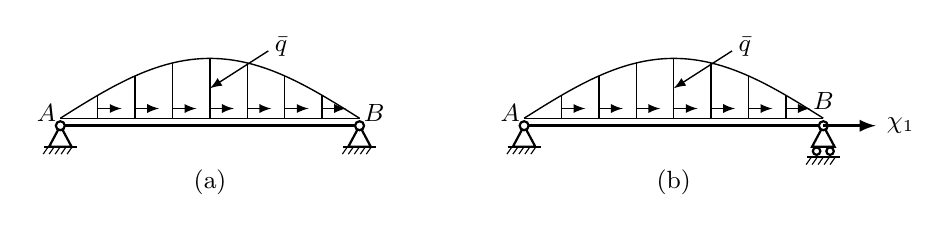
\begin{tikzpicture}[scale=0.95,>=latex,
				trave/.style={line width=1.2pt},
				carico/.style={black, line width=0.5pt},
				forza/.style={black, line width=1pt},
				]
				% ── Parametri vincoli (convenzione C06/C07) ──
				\def\tw{0.15}\def\thR{0.28}\def\rn{0.06}
				\def\rw{0.05}\def\bw{0.09}\def\gw{0.22}\def\hh{0.10}
				\def\Lb{4}        % lunghezza trave
				\def\hq{0.8}      % ordinata massima del carico (q-bar)
				\def\bb{0.10}     % quota della linea di base del carico (bordo cerniera)
				
				\def\hq{0.8}      % ordinata massima del carico (q-bar)
				\def\bb{0.10}     % quota della linea di base del carico (bordo cerniera)
				\def\fa{0.13}     % rialzo delle frecce rispetto alla linea di base
				
				% ── Cerniera in #1 ──
				\def\cerniera#1{%
					\draw[thick] (#1,0) -- (#1-\tw,-\thR) -- (#1+\tw,-\thR) -- cycle;
					\draw[thick] (#1-\gw,-\thR) -- (#1+\gw,-\thR);
					\foreach \x in {-0.16,-0.08,0,0.08,0.16}
					\draw[thin] (#1+\x,-\thR) -- ++(-0.07,-\hh);
					\draw[thick, fill=white] (#1,0) circle (\rn);}
				% ── Carrello verticale in #1 ──
				\def\carrello#1{%
					\draw[thick] (#1,0) -- (#1-\tw,-\thR) -- (#1+\tw,-\thR) -- cycle;
					\draw[thick] (#1-\bw,-\thR-\rw-0.01) circle (\rw);
					\draw[thick] (#1+\bw,-\thR-\rw-0.01) circle (\rw);
					\draw[thick] (#1-\gw,-\thR-2*\rw-0.04) -- (#1+\gw,-\thR-2*\rw-0.04);
					\foreach \x in {-0.16,-0.08,0,0.08,0.16}
					\draw[thin] (#1+\x,-\thR-2*\rw-0.04) -- ++(-0.07,-\hh);
					\draw[thick, fill=white] (#1,0) circle (\rn);}
				%			% ── Carico armonico longitudinale q(z)=qbar sin(pi z/l), verso +z ──
				\def\caricoarmonico{%
					% inviluppo (mezza sinusoide), chiuso sulla linea di base
					\draw[carico] plot[domain=0:\Lb, samples=90](\x, {\bb + \hq*sin(45*\x)});
					\draw[carico] (0,\bb) -- (\Lb,\bb);            % linea di base (chiusura)
					% ordinate (campitura): stazione centrale x=l/2 = massimo qbar
					\foreach \s in {0.5,1.0,1.5,2.0,2.5,3.0,3.5}
					\draw[carico] (\s,\bb) -- (\s, {\bb+\hq*sin(45*\s)});
					% frecce assiali, rialzate rispetto alla chiusura
					\foreach \s in {0.5,1.0,1.5,2.0,2.5,3.0,3.5}
					\draw[->, carico] (\s,{\bb+\fa}) -- (\s+0.32,{\bb+\fa});
					% q-bar (ordinata massima) con leader inclinato verso il tratto centrale
					\node[font=\small] at (2.95,{\bb+\hq+0.16}) {$\bar{q}$};
					\draw[carico, ->] (2.78,{\bb+\hq+0.10}) -- (2.0,{\bb+\hq/2});}
				
				% ===================== (a) trave incernierata =====================
				\begin{scope}[xshift=0cm]
					\draw[trave] (0,0) -- (\Lb,0);
					\cerniera{0}\cerniera{\Lb}
					\node[above left=-2pt, font=\small]  at (0,0)    {$A$};
					\node[above right=-2pt, font=\small] at (\Lb,0)  {$B$};
					\caricoarmonico
					\node[font=\small] at (\Lb/2,-0.75) {(a)};
				\end{scope}
				
				% ===================== (b) sistema principale =====================
				\begin{scope}[xshift=6.2cm]
					\draw[trave] (0,0) -- (\Lb,0);
					\cerniera{0}\carrello{\Lb}
					\node[above left=-2pt, font=\small] at (0,0) {$A$};
					\node[above=1pt, font=\small] at (\Lb,0.05) {$B$};
					\caricoarmonico
					\draw[->, forza] (\Lb,0) -- (\Lb+0.7,0);    % forza iperstatica
					\node[right, font=\small] at (\Lb+0.72,0) {$\chi_1$};
					\node[font=\small] at (\Lb/2,-0.75) {(b)};
				\end{scope}
				
			\end{tikzpicture}
			\caption{a)~trave incernierata con carico armonico longitudinale;
				b)~sistema principale scelto, con la cerniera in $B$ sostituita
				da un carrello verticale e dalla forza iperstatica $\chi_1 = H_B$.}
			\label{fig:stat_iper_long_01}
		\end{figure}
		
		
		
		
		
		\esottotit{Grado di iperstaticità.}
		La trave ha $m = 4$ reazioni (due componenti
		per ciascuna cerniera) e $n = 3$ equazioni di
		equilibrio globale: il grado di iperstaticità
		è $m - n = 1$. L'iperstaticità è di tipo
		longitudinale: entrambe le cerniere impediscono
		lo spostamento orizzontale, ma solo una
		reazione orizzontale è necessaria per
		l'equilibrio.
		
		\esottotit{Sistema principale}
		(\FIGref{fig:stat_iper_long_01}\,b).
		Si rimuove il vincolo orizzontale in $B$,
		ottenendo una trave con cerniera in $A$ e
		carrello verticale in $B$. L'incognita
		iperstatica è $\chi_1 = H_B$ (reazione
		orizzontale in $B$, positiva verso destra).
		La rimozione di un vincolo trasversale
		renderebbe il sistema degenere: la scelta
		è quindi obbligata nella componente
		longitudinale.
		
		\esottotit{Problema ``0'' --- carichi
			esterni}
		(\FIGref{fig:stat_iper_long_01-p0}\,a).
		Il sistema principale è soggetto al solo
		carico $q(z) = \bar{q}\sin(\pi z/\ell)$,
		con $\chi_1 = 0$.
		La risultante del carico è:
		\[
		R = \int_0^\ell \bar{q}\sin\frac{\pi z}{\ell}
		\,\dd z
		= \frac{2\bar{q}\ell}{\pi}.
		\]
		Dall'equilibrio longitudinale:
		$H_A = 2\bar{q}\ell/\pi$ (verso sinistra);
		per assenza di carichi trasversali:
		$V_A = V_B = 0$.
		
		\esottotit{Condizioni al contorno.}
		\[
		N_0(A) = H_A = \frac{2\bar{q}\ell}{\pi}
		\quad\text{(trazione)},
		\qquad
		N_0(B) = 0
		\quad\text{(bordo libero longitudinalmente)}.
		\]
		
		\begin{figure}[htbp]
			\centering
			\begin{tikzpicture}[scale=0.95,>=latex,
				trave/.style={line width=1.2pt},
				carico/.style={black, line width=0.5pt},
				diagN/.style={black, line width=0.8pt},
				hatch/.style={gray!40, line width=0.3pt},
				puntotang/.style={circle, fill=black, inner sep=1.1pt},
				]
				% ── Parametri ──
				\def\tw{0.15}\def\thR{0.28}\def\rn{0.06}
				\def\rw{0.05}\def\bw{0.09}\def\gw{0.22}\def\hh{0.10}
				\def\Lb{4}\def\hq{0.8}\def\bb{0.10}\def\fa{0.13}
				\def\hN{0.45}     % scala del diagramma N0 (qbar*l/pi -> hN)
				% ── Vincoli ──
				\def\cerniera#1{%
					\draw[thick] (#1,0) -- (#1-\tw,-\thR) -- (#1+\tw,-\thR) -- cycle;
					\draw[thick] (#1-\gw,-\thR) -- (#1+\gw,-\thR);
					\foreach \x in {-0.16,-0.08,0,0.08,0.16}
					\draw[thin] (#1+\x,-\thR) -- ++(-0.07,-\hh);
					\draw[thick, fill=white] (#1,0) circle (\rn);}
				\def\carrello#1{%
					\draw[thick] (#1,0) -- (#1-\tw,-\thR) -- (#1+\tw,-\thR) -- cycle;
					\draw[thick] (#1-\bw,-\thR-\rw-0.01) circle (\rw);
					\draw[thick] (#1+\bw,-\thR-\rw-0.01) circle (\rw);
					\draw[thick] (#1-\gw,-\thR-2*\rw-0.04) -- (#1+\gw,-\thR-2*\rw-0.04);
					\foreach \x in {-0.16,-0.08,0,0.08,0.16}
					\draw[thin] (#1+\x,-\thR-2*\rw-0.04) -- ++(-0.07,-\hh);
					\draw[thick, fill=white] (#1,0) circle (\rn);}
				% ── Carico armonico longitudinale ──
				\def\caricoarmonico{%
					\draw[carico] plot[domain=0:\Lb, samples=90] (\x, {\bb + \hq*sin(45*\x)});
					\draw[carico] (0,\bb) -- (\Lb,\bb);
					\foreach \s in {0.5,1.0,1.5,2.0,2.5,3.0,3.5}
					\draw[carico] (\s,\bb) -- (\s, {\bb+\hq*sin(45*\s)});
					\foreach \s in {0.5,1.0,1.5,2.0,2.5,3.0,3.5}
					\draw[->, carico] (\s,{\bb+\fa}) -- (\s+0.32,{\bb+\fa});
					\node[font=\small] at (2.95,{\bb+\hq+0.16}) {$\bar{q}$};
					\draw[carico, ->] (2.78,{\bb+\hq+0.10}) -- (2.0,{\bb+\hq/2});
				}
				
				% ===================== (a) sistema principale, solo carico =====================
				\begin{scope}[xshift=0cm]
					\draw[trave] (0,0) -- (\Lb,0);
					\cerniera{0}\carrello{\Lb}
					\node[above left=-2pt, font=\small] at (0,0) {$A$};
					\node[above=1pt, font=\small] at (\Lb,0.05) {$B$};
					\caricoarmonico
					\node[font=\small] at (\Lb/2,-0.75) {(a)};
				\end{scope}
				
				% ===================== (b) diagramma N0 (trazione, sopra l'asse) =====================
				\begin{scope}[xshift=6.2cm]
					\draw[trave] (0,0) -- (\Lb,0);
					% campitura
					\foreach \x in {0.1,0.3,...,3.9}
					\draw[hatch] (\x,0) -- (\x, {\hN*(1+cos(45*\x))});
					% contorno: chiusura verticale in A + curva 1+cos
					\draw[diagN] (0,0) -- (0,{2*\hN})
					plot[domain=0:\Lb, samples=100] (\x, {\hN*(1+cos(45*\x))});
					% flesso in mezzeria
					\node[puntotang] at (2,\hN) {};
					\cerniera{0}\carrello{\Lb}
					\node[above left=-2pt, font=\small] at (0,0) {$A$};
					\node[above right=-2pt, font=\small] at (\Lb,0) {$B$};
					\node[font=\small] at (1.0,0.42) {$\boldsymbol{\oplus}$};
					\node[left=-2pt, font=\small] at (0,{2*\hN}) {$\tfrac{2\bar{q}\ell}{\pi}$};
					\node[above, font=\scriptsize] at (2,\hN) {$\tfrac{\bar{q}\ell}{\pi}$};
					%\node[font=\small] at (2.9,0.55) {$N_0$};
					\node[font=\small] at (\Lb/2,-0.75) {(b)};
				\end{scope}
				
			\end{tikzpicture}
			\caption{(a)~problema ``0'': sistema principale soggetto al solo carico;
				(b)~sforzo normale $N_0$, in trazione, decrescente da $2\bar{q}\ell/\pi$
				in $A$ a zero in $B$, con flesso in mezzeria.}
			\label{fig:stat_iper_long_01-p0}
		\end{figure}
		
		
		
		
		
		\esottotit{Analisi qualitativa.}
		\begin{itemize}[nosep]
			\item $q = \bar{q}\sin(\pi z/\ell) \geq 0$
			su tutto $[0,\ell]$, quindi
			$N_0' = -q \leq 0$: $N_0$ è
			\emph{decrescente};
			\item $q'= \bar{q}(\pi/\ell)\cos(\pi z/\ell)$:
			in $A$ e in $B$ il carico ha pendenza
			massima, in mezzeria si annulla;
			quindi $N_0'' = -q'$ cambia segno
			in mezzeria: $N_0$ ha un flesso
			in $\ell/2$;
			\item $N_0(A) = 2\bar{q}\ell/\pi > 0$ e
			$N_0(B) = 0$: la trave è in trazione
			su tutto $[0,\ell]$.
		\end{itemize}
		
		\esottotit{Diagramma $N_0$.}
		Guardando a sinistra:
		\[
		N_0(z) = H_A - \int_0^z \bar{q}
		\sin\frac{\pi\zeta}{\ell}\,\dd\zeta
		= \frac{2\bar{q}\ell}{\pi}
		- \frac{\bar{q}\ell}{\pi}
		\!\left[1 - \cos\frac{\pi z}{\ell}
		\right]
		= \frac{\bar{q}\ell}{\pi}
		\!\left[1 + \cos\frac{\pi z}{\ell}
		\right].
		\]
		In accordo con l'analisi qualitativa:
		decrescente da $N_0(0) = 2\bar{q}\ell/\pi$
		a $N_0(\ell) = 0$, con flesso in mezzeria
		dove $N_0(\ell/2) = \bar{q}\ell/\pi$ (\FIGref{fig:stat_iper_long_01-p0}\,b).
		
		
		\esottotit{Problema ``1'' --- forza
			iperstatica unitaria}
		(\FIGref{fig:stat_iper_long_01-p1}\,a).
		Si applica $\chi_1 = H_B = 1$ verso destra,
		senza carichi esterni.
		Dall'equilibrio longitudinale:
		$H_A = 1$ (verso sinistra, discorde con
		$+z^e$); $V_A = V_B = 0$.
		
		\esottotit{Condizioni al contorno.}
		\[
		N_1(A) = H_A = 1 \quad\text{(trazione)},
		\qquad
		N_1(B) = H_B = 1 \quad\text{(trazione)}.
		\]
		
		\esottotit{Diagramma $N_1$.}
		Poiché $q = 0$, $N_1' = 0$ e $N_1$ è
		uniforme. Guardando a sinistra,
		$\mathcal{C}^-(z)$ contiene la sola
		reazione $H_A$ (discorde con $+z^e$):
		\[
		N_1(z) = H_A = 1
		\quad\text{(uniforme, trazione)}.
		\]
		In accordo con le condizioni al contorno.
		
		
		\begin{figure}[htbp]
			\centering
			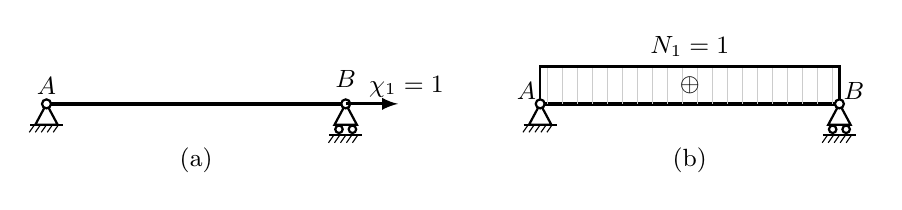
\begin{tikzpicture}[scale=0.95,>=latex,
				trave/.style={line width=1.2pt},
				forza/.style={black, line width=1pt},
				diagN/.style={black, line width=0.8pt},
				hatch/.style={gray!40, line width=0.3pt},
				]
				% ── Parametri ──
				\def\tw{0.15}\def\thR{0.28}\def\rn{0.06}
				\def\rw{0.05}\def\bw{0.09}\def\gw{0.22}\def\hh{0.10}
				\def\Lb{4}\def\hU{0.5}     % \hU = altezza del diagramma N1 (uniforme = 1)
				% ── Vincoli ──
				\def\cerniera#1{%
					\draw[thick] (#1,0) -- (#1-\tw,-\thR) -- (#1+\tw,-\thR) -- cycle;
					\draw[thick] (#1-\gw,-\thR) -- (#1+\gw,-\thR);
					\foreach \x in {-0.16,-0.08,0,0.08,0.16}
					\draw[thin] (#1+\x,-\thR) -- ++(-0.07,-\hh);
					\draw[thick, fill=white] (#1,0) circle (\rn);}
				\def\carrello#1{%
					\draw[thick] (#1,0) -- (#1-\tw,-\thR) -- (#1+\tw,-\thR) -- cycle;
					\draw[thick] (#1-\bw,-\thR-\rw-0.01) circle (\rw);
					\draw[thick] (#1+\bw,-\thR-\rw-0.01) circle (\rw);
					\draw[thick] (#1-\gw,-\thR-2*\rw-0.04) -- (#1+\gw,-\thR-2*\rw-0.04);
					\foreach \x in {-0.16,-0.08,0,0.08,0.16}
					\draw[thin] (#1+\x,-\thR-2*\rw-0.04) -- ++(-0.07,-\hh);
					\draw[thick, fill=white] (#1,0) circle (\rn);}
				
				% ===================== (a) sistema principale con la sola chi_1=1 =====================
				\begin{scope}[xshift=0cm]
					\draw[trave] (0,0) -- (\Lb,0);
					\cerniera{0}\carrello{\Lb}
					\node[above, font=\small] at (0,0) {$A$};
					\node[above=1pt, font=\small] at (\Lb,0.05) {$B$};
					\draw[->, forza] (\Lb,0) -- (\Lb+0.7,0);
					\node[above right=-1pt, font=\small] at (\Lb+0.22,0) {$\chi_1=1$};
					\node[font=\small] at (\Lb/2,-0.75) {(a)};
				\end{scope}
				
				% ===================== (b) diagramma N1 (uniforme, trazione, sopra l'asse) =====================
				\begin{scope}[xshift=6.6cm]
					\draw[trave] (0,0) -- (\Lb,0);
					\foreach \x in {0.1,0.3,...,3.9}\draw[hatch] (\x,0)--(\x,\hU);
					\draw[diagN] (0,0)--(0,\hU)--(\Lb,\hU)--(\Lb,0);
					\cerniera{0}\carrello{\Lb}
					\node[above left=-2pt, font=\small] at (0,0) {$A$};
					\node[above right=-2pt, font=\small] at (\Lb,0) {$B$};
					\node[font=\small] at (\Lb/2,0.5*\hU) {$\boldsymbol{\oplus}$};
					\node[above, font=\small] at (\Lb/2,\hU) {$N_1=1$};
					\node[font=\small] at (\Lb/2,-0.75) {(b)};
				\end{scope}
				
			\end{tikzpicture}
			\caption{a)~problema ``1'': forza iperstatica unitaria $\chi_1=1$ in $B$;
				b)~sforzo normale $N_1$, uniforme in trazione e pari a $1$.}
			\label{fig:stat_iper_long_01-p1}
		\end{figure}
		
		
		
		\esottotit{Soluzione generale}
		(\FIGref{fig:stat_iper_long_01-s}).
		Per sovrapposizione:
		\[
		N(z) = N_0(z) + \chi_1 N_1(z)
		= \frac{\bar{q}\ell}{\pi}
		\!\left[1 + \cos\frac{\pi z}{\ell}
		\right] + \chi_1.
		\]
		Le reazioni della soluzione generale sono:
		\[
		H_A = \frac{2\bar{q}\ell}{\pi} - \chi_1
		\quad\text{(verso sinistra)},
		\qquad
		H_B = \chi_1
		\quad\text{(verso destra)},
		\qquad
		V_A = V_B = 0.
		\]
		Ogni valore di $\chi_1$ identifica uno stato
		di sollecitazione staticamente ammissibile.
		La determinazione del valore effettivo di
		$\chi_1$ richiede l'imposizione della
		condizione di congruenza --- allungamento
		longitudinale totale nullo tra $A$ e $B$
		--- sviluppata nel Volume~II.
		
		\begin{figure}[htbp]
			\centering
			\begin{tikzpicture}[scale=0.95,>=latex,
				trave/.style={line width=1.2pt},
				carico/.style={black, line width=0.5pt},
				forza/.style={black, line width=1pt},
				diagN/.style={black, line width=0.8pt},
				hatch/.style={gray!40, line width=0.3pt},
				]
				% ── Parametri ──
				\def\tw{0.15}\def\thR{0.28}\def\rn{0.06}
				\def\rw{0.05}\def\bw{0.09}\def\gw{0.22}\def\hh{0.10}
				\def\Lb{4}\def\hq{0.8}\def\bb{0.10}\def\fa{0.13}
				\def\hz{0.4}      % scala di qbar*l/pi (gobba N0)
				\def\hx{0.4}      % livello di chi_1 (contributo N1*chi_1)
				% ── Vincoli ──
				\def\cerniera#1{%
					\draw[thick] (#1,0) -- (#1-\tw,-\thR) -- (#1+\tw,-\thR) -- cycle;
					\draw[thick] (#1-\gw,-\thR) -- (#1+\gw,-\thR);
					\foreach \x in {-0.16,-0.08,0,0.08,0.16}
					\draw[thin] (#1+\x,-\thR) -- ++(-0.07,-\hh);
					\draw[thick, fill=white] (#1,0) circle (\rn);}
				\def\carrello#1{%
					\draw[thick] (#1,0) -- (#1-\tw,-\thR) -- (#1+\tw,-\thR) -- cycle;
					\draw[thick] (#1-\bw,-\thR-\rw-0.01) circle (\rw);
					\draw[thick] (#1+\bw,-\thR-\rw-0.01) circle (\rw);
					\draw[thick] (#1-\gw,-\thR-2*\rw-0.04) -- (#1+\gw,-\thR-2*\rw-0.04);
					\foreach \x in {-0.16,-0.08,0,0.08,0.16}
					\draw[thin] (#1+\x,-\thR-2*\rw-0.04) -- ++(-0.07,-\hh);
					\draw[thick, fill=white] (#1,0) circle (\rn);}
				% ── Carico armonico longitudinale ──
				\def\caricoarmonico{%
					\draw[carico] plot[domain=0:\Lb, samples=90] (\x, {\bb + \hq*sin(45*\x)});
					\draw[carico] (0,\bb) -- (\Lb,\bb);
					\foreach \s in {0.5,1.0,1.5,2.0,2.5,3.0,3.5}
					\draw[carico] (\s,\bb) -- (\s, {\bb+\hq*sin(45*\s)});
					\foreach \s in {0.5,1.0,1.5,2.0,2.5,3.0,3.5}
					\draw[->, carico] (\s,{\bb+\fa}) -- (\s+0.32,{\bb+\fa});
					\node[font=\small] at (2.95,{\bb+\hq+0.16}) {$\bar{q}$};
					\draw[carico, ->] (2.78,{\bb+\hq+0.10}) -- (2.0,{\bb+\hq/2});}
				
				% ===================== (a) sistema principale: carico + chi_1 =====================
				\begin{scope}[xshift=0cm]
					\draw[trave] (0,0) -- (\Lb,0);
					\cerniera{0}\carrello{\Lb}
					\node[above left=-2pt, font=\small] at (0,0) {$A$};
					\node[above=1pt, font=\small] at (\Lb,0.05) {$B$};
					\caricoarmonico
					\draw[->, forza] (\Lb,0) -- (\Lb+0.7,0);
					\node[right, font=\small] at (\Lb+0.72,0) {$\chi_1$};
					\node[font=\small] at (\Lb/2,-0.75) {(a)};
				\end{scope}
				
				% ===================== (b) soluzione N = N0 + chi_1 N1 =====================
				\begin{scope}[xshift=6.6cm]
					\draw[trave] (0,0) -- (\Lb,0);
					% campitura (asse -> curva totale)
					\foreach \x in {0.1,0.3,...,3.9}
					\draw[hatch] (\x,0) -- (\x, {\hx + \hz*(1+cos(45*\x))});
					% contorno totale: chiusura in A, curva 1+cos traslata, chiusura in B
					\draw[diagN] (0,0) -- (0,{\hx+2*\hz})
					plot[domain=0:\Lb, samples=100] (\x, {\hx+\hz*(1+cos(45*\x))}) -- (\Lb,0);
					% livello chi_1 (contributo N1*chi_1)
					\draw[densely dashed, black, line width=0.5pt] (0,\hx) -- (\Lb,\hx);
					\cerniera{0}\carrello{\Lb}
					\node[left, font=\small] at (0,0) {$A$};
					\node[right=-1pt, font=\small] at (\Lb,0) {$B$};
					\node[font=\small] at (1.1,0.62) {$\boldsymbol{\oplus}$};
					\node[left=-3pt, font=\scriptsize] at (0,{\hx+\hz}) {$\tfrac{2\bar{q}\ell}{\pi}+\chi_1$};
					\node[right=1pt, font=\scriptsize] at (\Lb,\hx) {$\chi_1$};
					%\node[font=\small] at (2.95,0.72) {$N$};
					\node[font=\small] at (\Lb/2,-0.75) {(b)};
				\end{scope}
				
			\end{tikzpicture}
			\caption{a)~sistema principale soggetto al carico e alla forza
				iperstatica $\chi_1$; b)~sforzo normale $N = N_0 + \chi_1 N_1$,
				ottenuto traslando $N_0$ della costante $\chi_1$ (livello
				tratteggiato).}
			\label{fig:stat_iper_long_01-s}
		\end{figure}
	\end{svolgimento}
\end{esempio}

\subsection{Iperstaticità trasversale}

\begin{esempio}[Trave incastro-glifo con carico uniforme]
	Si consideri una trave piana di lunghezza $\ell$
	con incastro in $A$ e glifo di asse verticale
	in $B$, soggetta a un carico trasversale
	distribuito $p(z) = \bar{p}$ uniforme (verso
	il basso) su tutta la lunghezza
	(\FIGref{fig:stat_iper_trasv_01}\,a).
	Si costruiscano i diagrammi quotati di $T(z)$ e $M(z)$.
	
	\begin{svolgimento}
		
		\begin{figure}[htbp]
			\centering
			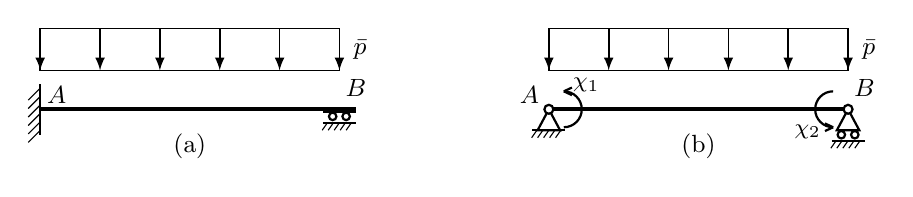
\begin{tikzpicture}[scale=0.95,>=latex,
				trave/.style={line width=1.4pt},
				carico/.style={black, line width=0.6pt},
				forza/.style={black, line width=0.8pt},
				]
				% ── Parametri ──
				\def\tw{0.15}\def\thR{0.28}\def\rn{0.06}
				\def\rw{0.05}\def\bw{0.09}\def\gw{0.22}\def\hh{0.10}
				\def\twall{0.16}\def\hwall{0.34}
				\def\Lell{4}\pgfmathsetmacro{\xMid}{0.5*\Lell}
				\def\pBot{0.52}\def\pTop{1.08}                 % riquadro del carico (chiusura sulle punte = \pBot)
				\def\rCoppia{0.24}\def\Lwing{0.12}\def\AoffX{0.20}\def\BoffX{0.20}
				% ── Vincoli ──
				\def\incastro#1{%
					\draw[thick] (#1,-\hwall) -- (#1,\hwall);
					\foreach \i in {-2.5,-1.5,-0.5,0.5,1.5,2.5}
					\draw[thin] (#1,{\i*\hwall/3}) -- ++(-\twall,-\twall);}
				\def\cerniera#1{%
					\draw[thick] (#1,0) -- (#1-\tw,-\thR) -- (#1+\tw,-\thR) -- cycle;
					\draw[thick] (#1-\gw,-\thR) -- (#1+\gw,-\thR);
					\foreach \x in {-0.16,-0.08,0,0.08,0.16}\draw[thin] (#1+\x,-\thR) -- ++(-0.07,-\hh);
					\draw[thick, fill=white] (#1,0) circle (\rn);}
				\def\carrello#1{%
					\draw[thick] (#1,0) -- (#1-\tw,-\thR) -- (#1+\tw,-\thR) -- cycle;
					\draw[thick] (#1-\bw,-\thR-\rw-0.01) circle (\rw);
					\draw[thick] (#1+\bw,-\thR-\rw-0.01) circle (\rw);
					\draw[thick] (#1-\gw,-\thR-2*\rw-0.04) -- (#1+\gw,-\thR-2*\rw-0.04);
					\foreach \x in {-0.16,-0.08,0,0.08,0.16}\draw[thin] (#1+\x,-\thR-2*\rw-0.04) -- ++(-0.07,-\hh);
					\draw[thick, fill=white] (#1,0) circle (\rn);}
				% ── Glifo: piatto rigido (no perno) + ruote + barra di terra (scorrimento orizzontale) ──
				\def\glifo#1{%
					\draw[thick] (#1-\gw,-0.03) -- (#1+\gw,-0.03);
					\draw[thick] (#1-\bw,-0.03-\rw-0.015) circle (\rw);
					\draw[thick] (#1+\bw,-0.03-\rw-0.015) circle (\rw);
					\draw[thick] (#1-\gw,-0.03-2*\rw-0.05) -- (#1+\gw,-0.03-2*\rw-0.05);
					\foreach \x in {-0.16,-0.08,0,0.08,0.16}\draw[thin] (#1+\x,-0.03-2*\rw-0.05) -- ++(-0.07,-\hh);}
				% ── Carico uniforme: riquadro chiuso (chiusura inferiore sulle punte), fino all'incastro ──
				\def\caricodist{%
					\draw[carico] (0,\pBot) rectangle (\Lell,\pTop);
					\foreach \x in {0,0.8,1.6,2.4,3.2,4.0}\draw[->, carico] (\x,\pTop) -- (\x,\pBot);
					\node[right, font=\small] at (\Lell+0.06,{0.5*(\pBot+\pTop)}) {$\bar{p}$};}
				% ── Coppie antiorarie che attraversano la trave (come mu_A, mu_B del template) ──
				\def\coppiaA#1{%
					\draw[forza] (\AoffX,-\rCoppia) arc[start angle=-90, end angle=90, radius=\rCoppia];
					\draw[forza] (\AoffX,\rCoppia) -- ({\AoffX+\Lwing*cos(25)},{\rCoppia+\Lwing*sin(25)});
					\draw[forza] (\AoffX,\rCoppia) -- ({\AoffX+\Lwing*cos(-25)},{\rCoppia+\Lwing*sin(-25)});
					\node[font=\footnotesize] at (\AoffX+0.3,\rCoppia+0.08) {#1};}
				\def\coppiaB#1{%
					\draw[forza] (\Lell-\BoffX,\rCoppia) arc[start angle=90, end angle=270, radius=\rCoppia];
					\draw[forza] (\Lell-\BoffX,-\rCoppia) -- ({\Lell-\BoffX+\Lwing*cos(155)},{-\rCoppia+\Lwing*sin(155)});
					\draw[forza] (\Lell-\BoffX,-\rCoppia) -- ({\Lell-\BoffX+\Lwing*cos(205)},{-\rCoppia+\Lwing*sin(205)});
					\node[font=\footnotesize] at (\Lell-\BoffX-\rCoppia-0.1,-0.30) {#1};}
				
				% ===================== (a) schema iniziale: incastro + glifo =====================
				\begin{scope}[xshift=0cm]
					\draw[trave] (0,0) -- (\Lell+\gw,0);     % trave estesa fino al bordo del piatto del glifo
					\incastro{0}\glifo{\Lell}
					\caricodist
					\node[above, font=\small] at (0.22,-0.05) {$A$};
					\node[above, font=\small] at (\Lell+\gw,0.04) {$B$};
					\node[font=\small] at (\xMid,-0.50) {(a)};
				\end{scope}
				
				% ===================== (b) sistema principale: cerniera + carrello + coppie =====================
				\begin{scope}[xshift=6.8cm]
					\draw[trave] (0,0) -- (\Lell,0);
					\cerniera{0}\carrello{\Lell}
					\caricodist
					\coppiaA{$\chi_1$}
					\coppiaB{$\chi_2$}
					\node[above left, font=\small] at (-0.,-0.05) {$A$};
					\node[above, font=\small] at (\Lell+\gw,0.04) {$B$};
					\node[font=\small] at (\xMid,-0.50) {(b)};
				\end{scope}
				
			\end{tikzpicture}
			\caption{Trave con incastro e glifo (a) e sistema principale scelto (b).}
			\label{fig:stat_iper_trasv_01}
		\end{figure}
		
		
		\esottotit{Grado di iperstaticità.}
		La trave ha $m = 5$ reazioni: tre all'incastro
		in $A$ ($H_A$, $V_A$, $\mu_A$) e due al glifo
		in $B$ ($V_B$, $\mu_B$). Con $n = 3$ equazioni
		di equilibrio globale, il grado di iperstaticità
		è $m - n = 2$. L'iperstaticità è di tipo
		trasversale: il carico è puramente trasversale
		e $H_A = N(z) = 0$ su tutta la trave.
		
		\esottotit{Sistema principale}
		(\FIGref{fig:stat_iper_trasv_01}\,b).
		Si rimuovono i vincoli rotazionali in $A$ e
		in $B$, ottenendo una trave con cerniera in
		$A$ e carrello verticale in $B$. Le incognite
		iperstatiche sono:
		\[
		\chi_1 = \mu_A \quad\text{(antioraria
			positiva)}, \qquad
		\chi_2 = \mu_B \quad\text{(antioraria
			positiva)}.
		\]
		
		\esottotit{Problema ``0'' --- carico
			uniforme sul sistema principale}
		(\FIGref{fig:stat_iper_trasv_01-p0}).
		
		\begin{figure}[htbp]
			\centering
			\resizebox{\textwidth}{!}{%
				\begin{tikzpicture}[
					scale=0.95,
					>=latex,
					trave/.style={line width=1.2pt},
					carico/.style={black, line width=0.4pt},
					forza/.style={black, line width=1pt},
					risultante/.style={gray!65, line width=1.8pt},
					diagT/.style={black, line width=0.8pt},
					diagM/.style={black, line width=0.8pt},
					diagTb/.style={gray!65, line width=1.0pt},
					diagMb/.style={gray!65, line width=1.0pt},
					hatch/.style={gray!40, line width=0.3pt},
					quota/.style={black, line width=0.4pt},
					fibre/.style={gray!70, line width=0.3pt},
					segno/.style={circle, draw=black, line width=0.4pt,
						minimum size=10pt, inner sep=0pt, font=\small\bfseries},
					]
					
					% ── Parametri dei vincoli (convenzione C06/C07) ──
					\def\tw{0.15}    \def\thR{0.28}   \def\rn{0.06}
					\def\rw{0.05}    \def\bw{0.09}    \def\gw{0.22}
					\def\hh{0.10}
					
					% ── Macro vincoli (riuso nei tre pannelli) ──
					\def\cerniera#1{%
						\draw[thick] (#1,0) -- (#1-\tw,-\thR) -- (#1+\tw,-\thR) -- cycle;
						\draw[thick] (#1-\gw,-\thR) -- (#1+\gw,-\thR);
						\foreach \xh in {-0.16,-0.08,0,0.08,0.16}{%
							\draw[thin] (#1+\xh,-\thR) -- ++(-0.07,-\hh);}
						\draw[thick, fill=white] (#1,0) circle (\rn);}
					\def\carrello#1{%
						\draw[thick] (#1,0) -- (#1-\tw,-\thR) -- (#1+\tw,-\thR) -- cycle;
						\draw[thick] (#1-\bw,-\thR-\rw-0.01) circle (\rw);
						\draw[thick] (#1+\bw,-\thR-\rw-0.01) circle (\rw);
						\draw[thick] (#1-\gw,-\thR-2*\rw-0.04) -- (#1+\gw,-\thR-2*\rw-0.04);
						\foreach \xh in {-0.16,-0.08,0,0.08,0.16}{%
							\draw[thin] (#1+\xh,-\thR-2*\rw-0.04) -- ++(-0.07,-\hh);}
						\draw[thick, fill=white] (#1,0) circle (\rn);}
					
					% ── Geometria del problema ──
					\def\Lell{4}
					\pgfmathsetmacro{\xA}{0}
					\pgfmathsetmacro{\xMid}{0.5*\Lell}      % mezzeria ℓ/2 = 2
					\def\yqi{-0.80}
					\def\ylab{-3.70}
					
					% ── Centri utili per le etichette (pre-calcolati per evitare ambiguità TikZ) ──
					\pgfmathsetmacro{\xMidAC}{0.5*\xMid}            % centro tratto AC
					\pgfmathsetmacro{\xMidCB}{0.5*(\xMid+\Lell)}    % centro tratto CB
					\pgfmathsetmacro{\xLabel}{0.5*\Lell}            % x dell'etichetta di pannello
					\pgfmathsetmacro{\yLabel}{0.4*\ylab}            % y dell'etichetta di pannello
					
					% ── Parametri del carico distribuito ──
					\def\pgap{0.10}
					\def\php{0.40}
					\pgfmathsetmacro{\pBase}{\pgap}
					\pgfmathsetmacro{\pTop}{\pgap+\php}
					
					% =========================================================
					% PANNELLO (a) — Schema statico: distribuito + risultante
					% =========================================================
					\begin{scope}[xshift=0cm]
						
						\draw[trave] (0,0) -- (\Lell,0);
						\draw[fibre, dashed] (0, -0.1) -- (\Lell, -0.1);
						
						% Cerniera in A
						\draw[thick] (0,0) -- (-\tw,-\thR) -- (\tw,-\thR) -- cycle;
						\draw[thick] (-\gw,-\thR) -- (\gw,-\thR);
						\foreach \x in {-0.16,-0.08,0,0.08,0.16}
						\draw[thin] (\x,-\thR) -- ++(-0.07,-\hh);
						
						% Carrello verticale in B
						\draw[thick] (\Lell,0) -- (\Lell-\tw,-\thR) -- (\Lell+\tw,-\thR) -- cycle;
						\draw[thick] (\Lell-\bw,-\thR-\rw-0.01) circle (\rw);
						\draw[thick] (\Lell+\bw,-\thR-\rw-0.01) circle (\rw);
						\draw[thick] (\Lell-\gw,-\thR-2*\rw-0.04) -- (\Lell+\gw,-\thR-2*\rw-0.04);
						\foreach \x in {-0.16,-0.08,0,0.08,0.16}
						\draw[thin] (\Lell+\x,-\thR-2*\rw-0.04) -- ++(-0.07,-\hh);
						
						\draw[thick, fill=white] (0,0) circle (\rn);
						\draw[thick, fill=white] (\Lell,0) circle (\rn);
						
						% Riquadro del carico distribuito p̄
						\draw[carico] (0,\pBase) rectangle (\Lell,\pTop);
						\foreach \x in {0.25, 0.75, 1.25, 1.75, 2.25, 2.75, 3.25, 3.75} {
							\draw[carico, -{Latex[length=2pt, width=1.5pt]}]
							(\x, \pTop) -- (\x, \pBase);
						}
						\node[above, font=\small] at (0.5, \pTop+0.02) {$\bar{p}$};
						
						
						\node[above left=-2pt,  font=\small] at (0,0)      {$A$};
						\node[above right=-2pt, font=\small] at (\Lell,0)  {$B$};
						%\node[below=2pt, font=\small] at (\xMid, 0) {$C$};
						
						
						\node[font=\small] at (\xLabel, \yLabel+0.25) {(a)};
						
					\end{scope}
					
					% =========================================================
					% PANNELLO (b) — Diagramma del taglio T(z)
					% =========================================================
					\begin{scope}[xshift=5.5cm]
						
						\draw[trave] (0,0) -- (\Lell,0);
						
						\cerniera{0}
						\carrello{\Lell}
						\node[above left=-2pt,  font=\small] at (0,0)      {$A$};
						\node[above right=-2pt, font=\small] at (\Lell,0)  {$B$};
						
						\def\sT{0.4}
						\pgfmathsetmacro{\Tmax}{(\Lell/2)*\sT}
						
						
						% Hatching del caso (a)
						\foreach \x in {0.10, 0.30, ..., 3.90} {
							\pgfmathsetmacro{\h}{(\Lell/2 - \x)*\sT}
							\draw[hatch] (\x, 0) -- (\x, \h);
						}
						
						% Caso (a) NERO: triangolo lineare
						\draw[diagT]
						(0, 0) -- (0, \Tmax)
						-- (\Lell, -\Tmax) -- (\Lell, 0);
						
						% ── Simboli ⊕/⊖ cerchiati nelle due zone ──
						\node[segno] at (\xMidAC/2, {0.4*\Tmax}) {$+$};
						\node[segno] at (1.20*\xMidCB, {-0.4*\Tmax}) {$-$};
						
						\node[left, font=\small] at (0., \Tmax-0.02) {$\tfrac{\bar{p}\ell}{2}$};
						\node[right, font=\small] at (\Lell, -\Tmax+0.02) {$\tfrac{\bar{p}\ell}{2}$};
						
						\node[font=\small] at (\xLabel, \yLabel+0.25) {(b)};
						
					\end{scope}
					
					% =========================================================
					% PANNELLO (c) — Diagramma del momento M(z)
					% =========================================================
					\begin{scope}[xshift=11.0cm]
						
						\draw[trave] (0,0) -- (\Lell,0);
						\cerniera{0}
						\carrello{\Lell}
						\node[above left=-2pt,  font=\small] at (0,0)      {$A$};
						\node[above right=-2pt, font=\small] at (\Lell,0)  {$B$};
						
						\def\sM{0.38}
						\pgfmathsetmacro{\Mb}{-(\Lell*\Lell/4)*\sM}
						\pgfmathsetmacro{\Ma}{-(\Lell*\Lell/8)*\sM}
						
						
						% Hatching del caso (a) — parabola
						\foreach \x in {0.10, 0.30, ..., 3.90} {
							\pgfmathsetmacro{\h}{(\x*(\Lell-\x)/(\Lell*\Lell/4))*\Ma}
							\draw[hatch] (\x, 0) -- (\x, \h);
						}
						
						% Caso (a) NERO: parabola
						\draw[diagM]
						(0.00, 0)
						\foreach \x in {0.20, 0.40, ..., 3.80} {
							-- ({\x}, {(\x*(\Lell-\x)/(\Lell*\Lell/4))*\Ma})
						}
						-- (\Lell, 0);
						
						\node[above, font=\small] at (\xMid, \Ma+0.02) {$\tfrac{\bar{p}\ell^2}{8}$};
						%\node[above, font=\small, gray!50!black] at (\xMid, \Mb+0.02) 	{$\tfrac{\bar{p}\ell^2}{4}$};
						
						% Tangente al vertice della parabola — parallela alla corda A–B (l'asse).
						% Visualizza la proprietà di tangenza in mezzeria nel caso degenere
						% M(A)=M(B)=0: corda coincide con l'asse, tangente in mezzeria orizzontale.
						\draw[diagMb, dashed] (\Lell/5,\Ma) -- (4*\Lell/5,\Ma);
						
						\node[font=\small] at (\xLabel, \yLabel+0.25) {(c)};
						
					\end{scope}
					
				\end{tikzpicture}
			}
			\caption{Problema ``0'': carico uniforme
				sul sistema principale (a); taglio
				$T_0$ (b); momento $M_0$ (c).}
			\label{fig:stat_iper_trasv_01-p0}
		\end{figure}
		
		
		Trave appoggiata con carico uniforme $\bar{p}$
		(esempio già svolto nel
		\PARref{sec:esempi_trasversale}).
		Reazioni: $V_A = V_B = \bar{p}\ell/2$
		(verso l'alto).
		
		\esottotit{Condizioni al contorno.}
		\[
		T_0(A) = \frac{\bar{p}\ell}{2}, \quad
		M_0(A) = 0, \quad
		T_0(B) = -\frac{\bar{p}\ell}{2}, \quad
		M_0(B) = 0.
		\]
		
		Diagrammi:
		\[
		T_0(z) = \bar{p}\!\left(\frac{\ell}{2} - z\right),
		\qquad
		M_0(z) = \frac{\bar{p}}{2}z(\ell - z).
		\]
		Massimo in mezzeria: $M_0(\ell/2) =
		\bar{p}\ell^2/8$.
		
		\esottotit{Problema ``1'' --- coppia
			unitaria in $A$}
		(\FIGref{fig:stat_iper_trasv_01-p1}).
		
		
		\begin{figure}[htbp]
			\centering
			\resizebox{\textwidth}{!}{%
				\begin{tikzpicture}[scale=0.95,>=latex,
					trave/.style={line width=1.4pt},
					forza/.style={black, line width=0.8pt},
					diagT/.style={black, line width=0.6pt},
					diagM/.style={black, line width=0.6pt},
					hatch/.style={gray!50, line width=0.3pt},
					quota/.style={black, line width=0.4pt},
					fibre/.style={gray!70, line width=0.3pt},
					]
					\def\tw{0.15}\def\thR{0.28}\def\rn{0.06}
					\def\rw{0.05}\def\bw{0.09}\def\gw{0.22}\def\hh{0.10}
					\def\Lell{4}\pgfmathsetmacro{\xMid}{0.5*\Lell}
					\def\yqi{-0.80}\def\ylab{-1.35}
					\def\rCoppia{0.25}\def\Lwing{0.12}\def\AoffX{0.20}\def\BoffX{0.20}
					% ── trave + cerniera A + carrello B + perni + etichette ──
					\def\vincoli{%
						\draw[thick] (0,0) -- (-\tw,-\thR) -- (\tw,-\thR) -- cycle;
						\draw[thick] (-\gw,-\thR) -- (\gw,-\thR);
						\foreach \x in {-0.16,-0.08,0,0.08,0.16}\draw[thin] (\x,-\thR) -- ++(-0.07,-\hh);
						\draw[thick] (\Lell,0) -- (\Lell-\tw,-\thR) -- (\Lell+\tw,-\thR) -- cycle;
						\draw[thick] (\Lell-\bw,-\thR-\rw-0.01) circle (\rw);
						\draw[thick] (\Lell+\bw,-\thR-\rw-0.01) circle (\rw);
						\draw[thick] (\Lell-\gw,-\thR-2*\rw-0.04) -- (\Lell+\gw,-\thR-2*\rw-0.04);
						\foreach \x in {-0.16,-0.08,0,0.08,0.16}\draw[thin] (\Lell+\x,-\thR-2*\rw-0.04) -- ++(-0.07,-\hh);
						\draw[thick, fill=white] (0,0) circle (\rn);
						\draw[thick, fill=white] (\Lell,0) circle (\rn);
						\node[above left=-2pt, font=\small] at (0,0) {$A$};
						\node[above right=-2pt, font=\small] at (\Lell,0) {$B$};}
					% ── coppia antioraria in A ──
					\def\coppiaA#1{%
						\draw[forza] (\AoffX,-\rCoppia) arc[start angle=-90, end angle=90, radius=\rCoppia];
						\draw[forza] (\AoffX,\rCoppia) -- ({\AoffX+\Lwing*cos(25)},{\rCoppia+\Lwing*sin(25)});
						\draw[forza] (\AoffX,\rCoppia) -- ({\AoffX+\Lwing*cos(-25)},{\rCoppia+\Lwing*sin(-25)});
						\node[right, font=\footnotesize] at (\AoffX+\rCoppia+0.02,0.16) {#1};}
					
					% (a) schema: sola coppia chi_1=1 in A
					\begin{scope}[xshift=0cm]
						\draw[trave] (0,0) -- (\Lell,0);
						\draw[fibre, dashed] (0,-0.1) -- (\Lell,-0.1);
						\vincoli
						\coppiaA{$\chi_1=1$}
						\node[font=\small] at (\xMid,\ylab/2) {(a)};
					\end{scope}
					% (b) T_1 = 1/l uniforme
					\begin{scope}[xshift=5.5cm]
						\draw[trave] (0,0) -- (\Lell,0);
						\def\Tf{0.45}
						\foreach \x in {0.10,0.30,...,3.90}\draw[hatch] (\x,0) -- (\x,\Tf);
						\draw[diagT] (0,0) -- (0,\Tf) -- (\Lell,\Tf) -- (\Lell,0);
						\vincoli
						\node[font=\small] at (\xMid,{0.5*\Tf}) {$\boldsymbol{\oplus}$};
						\node[font=\small] at (3.75,{\Tf+0.30}) {$\tfrac{1}{\ell}$};
						\draw[quota, ->] (3.55,{\Tf+0.20}) -- (3.3,{0.5*\Tf});
						
						\node[font=\small] at (\xMid,\ylab/2) {(b)};
					\end{scope}
					% (c) M_1: da -1 in A (sopra l'asse) a 0 in B
					\begin{scope}[xshift=11.0cm]
						\draw[trave] (0,0) -- (\Lell,0);
						\def\hM{0.7}
						\foreach \x in {0.10,0.30,...,3.90}{\pgfmathsetmacro{\h}{\hM*(1-\x/\Lell)}\draw[hatch] (\x,0)--(\x,\h);}
						\draw[diagM] (0,0) -- (0,\hM) -- (\Lell,0);
						\vincoli
						\node[left, font=\small] at (0,\hM+0.02) {$1$};
						\node[font=\small] at (\xMid,\ylab/2) {(c)};
					\end{scope}
				\end{tikzpicture}
			}
			\caption{Problema ``1'': coppia unitaria in $A$ (a);
				taglio $T_1$ (b); momento $M_1$ (c).}
			\label{fig:stat_iper_trasv_01-p1}
		\end{figure}
		
		
		Trave appoggiata con coppia antioraria
		$\mu(A) = 1$ in $A$, senza carichi esterni
		(esempio già svolto nella
		\PARref{sec:esempi_trasversale}).
		Reazioni: $V_A = 1/\ell$ (verso l'alto),
		$V_B = 1/\ell$ (verso il basso).
		
		\esottotit{Condizioni al contorno.}
		\[
		T_1(A) = \frac{1}{\ell}, \quad
		M_1(A) = -1, \quad
		T_1(B) = \frac{1}{\ell}, \quad
		M_1(B) = 0.
		\]
		
		Diagrammi ($T_1$ uniforme, $M_1$ lineare):
		\[
		T_1(z) = \frac{1}{\ell},
		\qquad
		M_1(z) = -1 + \frac{z}{\ell}.
		\]
		
		\esottotit{Problema ``2'' --- coppia
			unitaria in $B$}
		(\FIGref{fig:stat_iper_trasv_01-p2}).
		
		\begin{figure}[htbp]
			\centering
			\resizebox{\textwidth}{!}{%
				\begin{tikzpicture}[scale=0.95,>=latex,
					trave/.style={line width=1.4pt},
					forza/.style={black, line width=0.8pt},
					diagT/.style={black, line width=0.6pt},
					diagM/.style={black, line width=0.6pt},
					hatch/.style={gray!50, line width=0.3pt},
					quota/.style={black, line width=0.4pt},
					fibre/.style={gray!70, line width=0.3pt},
					]
					\def\tw{0.15}\def\thR{0.28}\def\rn{0.06}
					\def\rw{0.05}\def\bw{0.09}\def\gw{0.22}\def\hh{0.10}
					\def\Lell{4}\pgfmathsetmacro{\xMid}{0.5*\Lell}
					\def\yqi{-0.80}\def\ylab{-1.35}
					\def\rCoppia{0.25}\def\Lwing{0.12}\def\AoffX{0.20}\def\BoffX{0.20}
					\def\vincoli{%
						\draw[thick] (0,0) -- (-\tw,-\thR) -- (\tw,-\thR) -- cycle;
						\draw[thick] (-\gw,-\thR) -- (\gw,-\thR);
						\foreach \x in {-0.16,-0.08,0,0.08,0.16}\draw[thin] (\x,-\thR) -- ++(-0.07,-\hh);
						\draw[thick] (\Lell,0) -- (\Lell-\tw,-\thR) -- (\Lell+\tw,-\thR) -- cycle;
						\draw[thick] (\Lell-\bw,-\thR-\rw-0.01) circle (\rw);
						\draw[thick] (\Lell+\bw,-\thR-\rw-0.01) circle (\rw);
						\draw[thick] (\Lell-\gw,-\thR-2*\rw-0.04) -- (\Lell+\gw,-\thR-2*\rw-0.04);
						\foreach \x in {-0.16,-0.08,0,0.08,0.16}\draw[thin] (\Lell+\x,-\thR-2*\rw-0.04) -- ++(-0.07,-\hh);
						\draw[thick, fill=white] (0,0) circle (\rn);
						\draw[thick, fill=white] (\Lell,0) circle (\rn);
						\node[above left=-2pt, font=\small] at (0,0) {$A$};
						\node[above right=-2pt, font=\small] at (\Lell,0) {$B$};}
					% ── coppia antioraria in B ──
					\def\coppiaB#1{%
						\draw[forza] (\Lell-\BoffX,\rCoppia) arc[start angle=90, end angle=270, radius=\rCoppia];
						\draw[forza] (\Lell-\BoffX,-\rCoppia) -- ({\Lell-\BoffX+\Lwing*cos(155)},{-\rCoppia+\Lwing*sin(155)});
						\draw[forza] (\Lell-\BoffX,-\rCoppia) -- ({\Lell-\BoffX+\Lwing*cos(205)},{-\rCoppia+\Lwing*sin(205)});
						\node[left, font=\footnotesize] at (\Lell-\BoffX-\rCoppia-0.02,0.16) {#1};}
					
					% (a) schema: sola coppia chi_2=1 in B
					\begin{scope}[xshift=0cm]
						\draw[trave] (0,0) -- (\Lell,0);
						\draw[fibre, dashed] (0,-0.1) -- (\Lell,-0.1);
						\vincoli
						\coppiaB{$\chi_2=1$}
						\node[font=\small] at (\xMid,\ylab/2) {(a)};
					\end{scope}
					% (b) T_2 = 1/l uniforme
					\begin{scope}[xshift=5.5cm]
						\draw[trave] (0,0) -- (\Lell,0);
						\def\Tf{0.45}
						\foreach \x in {0.10,0.30,...,3.90}\draw[hatch] (\x,0) -- (\x,\Tf);
						\draw[diagT] (0,0) -- (0,\Tf) -- (\Lell,\Tf) -- (\Lell,0);
						\vincoli
						\node[font=\small] at (\xMid,{0.5*\Tf}) {$\boldsymbol{\oplus}$};
						%\node[above, font=\small] at (\Lell-0.35,\Tf) {$\tfrac{1}{\ell}$};
						
						\node[font=\small] at (3.75,{\Tf+0.30}) {$\tfrac{1}{\ell}$};
						\draw[quota, ->] (3.55,{\Tf+0.20}) -- (3.3,{0.5*\Tf});
						
						
						\node[font=\small] at (\xMid,\ylab/2) {(b)};
					\end{scope}
					% (c) M_2: da 0 in A a +1 in B (sotto l'asse)
					\begin{scope}[xshift=11.0cm]
						\draw[trave] (0,0) -- (\Lell,0);
						\def\hM{0.7}
						\foreach \x in {0.10,0.30,...,3.90}{\pgfmathsetmacro{\h}{-\hM*(\x/\Lell)}\draw[hatch] (\x,0)--(\x,\h);}
						\draw[diagM] (0,0) -- (\Lell,-\hM) -- (\Lell,0);
						\vincoli
						\node[right, font=\small] at (\Lell,-\hM-0.02) {$1$};
						\node[font=\small] at (\xMid,\ylab/2) {(c)};
					\end{scope}
				\end{tikzpicture}
			}
			\caption{Problema ``2'': coppia unitaria in $B$ (a);
				taglio $T_2$ (b); momento $M_2$ (c).}
			\label{fig:stat_iper_trasv_01-p2}
		\end{figure}
		

		Trave appoggiata con coppia antioraria
		$\mu(B) = 1$ in $B$, senza carichi esterni
		(esempio già svolto nella
		\PARref{sec:esempi_trasversale}).
		Reazioni: $V_A = 1/\ell$ (verso l'alto),
		$V_B = 1/\ell$ (verso il basso).
		
		\esottotit{Condizioni al contorno.}
		\[
		T_2(A) = \frac{1}{\ell}, \quad
		M_2(A) = 0, \quad
		T_2(B) = \frac{1}{\ell}, \quad
		M_2(B) = 1.
		\]
		
		Diagrammi ($T_2$ uniforme, $M_2$ lineare):
		\[
		T_2(z) = \frac{1}{\ell},
		\qquad
		M_2(z) = \frac{z}{\ell}.
		\]
		
		\esottotit{Osservazione.}
		Le reazioni dei problemi ``1'' e ``2'' sono
		identiche: $V_A = 1/\ell$ verso l'alto e
		$V_B = 1/\ell$ verso il basso in entrambi
		i casi. Anche i diagrammi di $T_1$ e $T_2$
		coincidono. La differenza risiede
		esclusivamente nella posizione della coppia
		concentrata, che si riflette nei valori
		alle estremità di $M_1$ e $M_2$:
		$M_1(A) = -1$, $M_1(B) = 0$;
		$M_2(A) = 0$, $M_2(B) = 1$.
		
		\esottotit{Soluzione generale}
		(\FIGref{fig:stat_iper_trasv_01-s}).
		
		
		\begin{figure}[htbp]
			\centering
			\resizebox{\textwidth}{!}{%
				\begin{tikzpicture}[scale=0.95,>=latex,
					trave/.style={line width=1.4pt},
					carico/.style={black, line width=0.6pt},
					forza/.style={black, line width=0.8pt},
					diagT/.style={black, line width=0.7pt},
					diagM/.style={black, line width=0.7pt},
					hatch/.style={gray!50, line width=0.3pt},
					rif/.style={densely dashed, black, line width=0.5pt},
					quota/.style={black, line width=0.4pt},
					]
					\def\tw{0.15}\def\thR{0.28}\def\rn{0.06}
					\def\rw{0.05}\def\bw{0.09}\def\gw{0.22}\def\hh{0.10}
					\def\Lell{4}\pgfmathsetmacro{\xMid}{0.5*\Lell}
					\def\pBot{0.45}\def\pTop{0.95}
					\def\rCoppia{0.24}\def\Lwing{0.12}\def\AoffX{0.20}\def\BoffX{0.20}
					\def\ylab{-1.55}
					\def\cerniera#1{%
						\draw[thick] (#1,0) -- (#1-\tw,-\thR) -- (#1+\tw,-\thR) -- cycle;
						\draw[thick] (#1-\gw,-\thR) -- (#1+\gw,-\thR);
						\foreach \x in {-0.16,-0.08,0,0.08,0.16}\draw[thin] (#1+\x,-\thR) -- ++(-0.07,-\hh);
						\draw[thick, fill=white] (#1,0) circle (\rn);}
					\def\carrello#1{%
						\draw[thick] (#1,0) -- (#1-\tw,-\thR) -- (#1+\tw,-\thR) -- cycle;
						\draw[thick] (#1-\bw,-\thR-\rw-0.01) circle (\rw);
						\draw[thick] (#1+\bw,-\thR-\rw-0.01) circle (\rw);
						\draw[thick] (#1-\gw,-\thR-2*\rw-0.04) -- (#1+\gw,-\thR-2*\rw-0.04);
						\foreach \x in {-0.16,-0.08,0,0.08,0.16}\draw[thin] (#1+\x,-\thR-2*\rw-0.04) -- ++(-0.07,-\hh);
						\draw[thick, fill=white] (#1,0) circle (\rn);}
					\def\caricodist{%
						\draw[carico] (0,\pBot) rectangle (\Lell,\pTop);
						\foreach \x in {0,0.8,1.6,2.4,3.2,4.0}\draw[->, carico] (\x,\pTop) -- (\x,\pBot);
						\node[right, font=\small] at (\Lell+0.06,{0.5*(\pBot+\pTop)}) {$\bar{p}$};}
					\def\coppiaA#1{%
						\draw[forza] (\AoffX,-\rCoppia) arc[start angle=-90, end angle=90, radius=\rCoppia];
						\draw[forza] (\AoffX,\rCoppia) -- ({\AoffX+\Lwing*cos(25)},{\rCoppia+\Lwing*sin(25)});
						\draw[forza] (\AoffX,\rCoppia) -- ({\AoffX+\Lwing*cos(-25)},{\rCoppia+\Lwing*sin(-25)});
						\node[font=\footnotesize] at (\AoffX+0.28,\rCoppia+0.06) {#1};}
					\def\coppiaB#1{%
						\draw[forza] (\Lell-\BoffX,\rCoppia) arc[start angle=90, end angle=270, radius=\rCoppia];
						\draw[forza] (\Lell-\BoffX,-\rCoppia) -- ({\Lell-\BoffX+\Lwing*cos(155)},{-\rCoppia+\Lwing*sin(155)});
						\draw[forza] (\Lell-\BoffX,-\rCoppia) -- ({\Lell-\BoffX+\Lwing*cos(205)},{-\rCoppia+\Lwing*sin(205)});
						\node[font=\footnotesize] at (\Lell-\BoffX-\rCoppia-0.10,-0.30) {#1};}
					
					% ===== (a) sistema principale =====
					\begin{scope}[xshift=0cm]
						\draw[trave] (0,0) -- (\Lell,0);
						\cerniera{0}\carrello{\Lell}
						\caricodist
						\coppiaA{$\chi_1$}\coppiaB{$\chi_2$}
						\node[above left, font=\small] at (0,0.04) {$A$};
						\node[above right=-1pt, font=\small] at (\Lell,0.04) {$B$};
						\node[font=\small] at (\xMid/2,\ylab/2) {(a)};
					\end{scope}
					% ===== (b) T = T_0 + (chi1+chi2)/l =====
					\begin{scope}[xshift=6.0cm]
						\def\kT{2.0}                              % zoom del pannello taglio
						\pgfmathsetmacro{\hT}{0.42*\kT}           % p l /2
						\pgfmathsetmacro{\cT}{\hT/3}              % (chi1+chi2)/l = (1/3)(p l /2)  [chi=p l^2/12]
						\draw[trave] (0,0) -- (\Lell,0);
						\foreach \x in {0.1,0.3,...,3.9}{\pgfmathsetmacro{\h}{\cT+\hT*(1-2*\x/\Lell)}\draw[hatch] (\x,0)--(\x,\h);}
						\draw[diagT] (0,0)--(0,{\cT+\hT}) -- (\Lell,{\cT-\hT}) -- (\Lell,0);
						\draw[rif] (0,\cT)--(\Lell,\cT);
						\cerniera{0}\carrello{\Lell}
						\node[above left, font=\small] at (0,0.04) {$A$};
						\node[above right=-1pt, font=\small] at (\Lell,0.04) {$B$};
						\node[font=\footnotesize] at (0.5,0.55) {$\boldsymbol{\oplus}$};
						\node[font=\footnotesize] at (3.55,-0.18) {$\boldsymbol{\ominus}$};
						% trattini di richiamo ai valori estremi e alla costante
						\draw[quota, <-] (0,{0.55*(\cT+\hT)}) -- (0.55,{\cT+\hT+0.30});
						\node[right, font=\scriptsize] at (0.52,{\cT+\hT+0.30}) {$\tfrac{\bar p\ell}{2}+\tfrac{\chi_1+\chi_2}{\ell}$};
						\draw[quota, <-] (\Lell,{\cT-\hT/2}) -- (\Lell-1.0,{\cT-\hT/2-0.50});
						\node[below left=-3pt, font=\scriptsize] at (\Lell+0.16,{\cT-\hT-0.14}) {$-\tfrac{\bar p\ell}{2}+\tfrac{\chi_1+\chi_2}{\ell}$};
						\draw[quota, <-] (2.55,\cT) -- (2.55,{\cT+0.34});
						\node[above, font=\scriptsize] at (2.55,{\cT+0.32}) {$\tfrac{\chi_1+\chi_2}{\ell}$};
						\node[font=\small] at (\xMid/2,\ylab/2) {(b)};
					\end{scope}
					% ===== (c) M = M_0 + retta di chiusura =====
					\begin{scope}[xshift=12.0cm]
						\def\kM{1.5}                              % zoom del pannello momento
						\pgfmathsetmacro{\sag}{0.52*\kM}          % p l^2/8
						\pgfmathsetmacro{\mA}{2*\sag/3}           % chi_1 = (2/3)(p l^2/8)  [chi=p l^2/12]
						\pgfmathsetmacro{\mB}{2*\sag/3}           % chi_2
						\draw[trave] (0,0) -- (\Lell,0);
						\foreach \x in {0.1,0.3,...,3.9}{\pgfmathsetmacro{\u}{\x/\Lell}\pgfmathsetmacro{\h}{\mA-(\mA+\mB)*\u-\sag*4*\u*(1-\u)}\draw[hatch] (\x,0)--(\x,\h);}
						\draw[diagM] (0,0)--(0,\mA) plot[domain=0:\Lell,samples=90] (\x,{\mA-(\mA+\mB)*(\x/\Lell)-\sag*4*(\x/\Lell)*(1-\x/\Lell)}) -- (\Lell,0);
						\draw[rif] (0,\mA)--(\Lell,-\mB);
						\cerniera{0}\carrello{\Lell}
						\node[above left, font=\small] at (0,0.04) {$A$};
						\node[above right=-1pt, font=\small] at (\Lell,0.04) {$B$};
						\draw[<->, quota] (\xMid,{(\mA-\mB)/2})--(\xMid,{(\mA-\mB)/2-\sag});
						\node[right, font=\scriptsize] at (\xMid+0.05,{(\mA-\mB)/2-0.5*\sag}) {$\tfrac{\bar p\ell^2}{8}$};
						\node[above, font=\scriptsize] at (0,\mA+0.02) {$-\chi_1$};
						\node[right, font=\scriptsize] at (\Lell+0.06,-\mB-0.02) {$\chi_2$};
						\node[font=\small] at (\xMid/2,\ylab/2) {(c)};
					\end{scope}
				\end{tikzpicture}
			}
			\caption{Soluzione generale (sistema principale, a): taglio
				$T = T_0 + \chi_1 T_1 + \chi_2 T_2$ (b), retta $T_0$ traslata
				della costante $(\chi_1+\chi_2)/\ell$; momento
				$M = M_0 + \chi_1 M_1 + \chi_2 M_2$ (c), parabola $M_0$ appesa
				alla retta di chiusura da $-\chi_1$ in $A$ a $\chi_2$ in $B$.
				I diagrammi (b)--(c) sono tracciati per la scelta illustrativa
				$\chi_1 = \chi_2 = \bar p\,\ell^2/12$; i valori effettivi si
				ottengono imponendo la congruenza (Vol.~II).}
			\label{fig:stat_iper_trasv_01-s}
		\end{figure}
		
		

		Per sovrapposizione:
		\[
		T(z) = \bar{p}\!\left(\frac{\ell}{2} - z\right)
		+ \frac{\chi_1 + \chi_2}{\ell},
		\qquad 
		M(z) = \frac{\bar{p}}{2}z(\ell - z)
		+ \left(\frac{z}{\ell} - 1\right)\chi_1
		+ \frac{z}{\ell}\,\chi_2.
		\]
		Ogni coppia di valori $(\chi_1, \chi_2)$
		identifica uno stato di sollecitazione
		staticamente ammissibile. La determinazione
		dei valori effettivi richiede l'imposizione
		delle condizioni di congruenza --- rotazioni
		nulle in $A$ e in $B$ --- sviluppate nel
		Volume~II.
		
	\end{svolgimento}
\end{esempio}


\subsection{Problema statico misto}
\label{sec:esempi_misto_iper}

\begin{esempio}[Trave iperstatica con glifo inclinato]
	Si consideri una trave piana di lunghezza $\ell$
	con incastro in $A$ e glifo in $B$ con piano di
	scorrimento inclinato di $\pi/4$ rispetto
	all'orizzontale, soggetta a due forze concentrate
	$Y(C) = Y(D) = P$ (verso il basso) applicate in
	$C$ $(z = \ell/3)$ e in $D$ $(z = 2\ell/3)$
	(\FIGref{fig:stat_misto_iper_01}\,a).
	Si costruiscano i diagrammi quotati di $N(z)$, $T(z)$
	e $M(z)$.
	
	\begin{svolgimento}
		
		
		\begin{figure}[htbp]
			\centering
			\resizebox{0.85\textwidth}{!}{%
				\begin{tikzpicture}[>=Stealth, line width=0.8pt,
					forza/.style={line width=0.8pt},          % tratto semplice: la freccia e' manuale (alette)
					carico/.style={->, line width=0.8pt},      % forze concentrate P
					quota/.style={line width=0.4pt},
					hatch/.style={line width=0.3pt, gray!50},
					rif/.style={line width=0.5pt}]
					
					\def\Lell{3.6}\def\Lc{1.2}\def\Ld{2.4}
					\def\rCoppia{0.24}\def\Lwing{0.12}\def\AoffX{0.20}\def\BoffX{0.20}
					
					% --- vincoli e indicatore pi/4 (sposta nel preambolo se vuoi) ---
					\newcommand\incastro[1]{%
						\draw[line width=1.0pt] (#1)+(0,-0.34) -- ($(#1)+(0,0.34)$);
						\foreach \yy in {-0.30,-0.18,-0.06,0.06,0.18,0.30}{\draw[hatch] ($(#1)+(0,\yy)$) -- ($(#1)+(-0.16,\yy-0.16)$);}}
					\newcommand\cerniera[1]{%
						\begin{scope}[shift={(#1)}]
							\draw[thick] (0,0) -- (-0.22,-0.38) -- (0.22,-0.38) -- cycle;
							\draw[thick] (-0.32,-0.38) -- (0.32,-0.38);
							\foreach \x in {-0.24,-0.12,0,0.12,0.24}{\draw[hatch] (\x,-0.38) -- (\x-0.12,-0.52);}
						\end{scope}
						\node[circle, fill=white, draw=black, inner sep=0pt, minimum size=5pt, line width=0.8pt] at (#1) {};}
					\newcommand\carrelloincl[1]{%
						\begin{scope}[shift={(#1)}, rotate=45]
							\draw[thick] (0,0) -- (-0.22,-0.38) -- (0.22,-0.38) -- cycle;
							\draw[thick] (-0.15,-0.45) circle (0.06); \draw[thick] (0.15,-0.45) circle (0.06);
							\draw[thick] (-0.32,-0.53) -- (0.32,-0.53);
							\foreach \x in {-0.24,-0.12,0,0.12,0.24}{\draw[hatch] (\x,-0.53) -- (\x-0.12,-0.67);}
						\end{scope}
						\node[circle, fill=white, draw=black, inner sep=0pt, minimum size=5pt, line width=0.8pt] at (#1) {};}
					\newcommand\glifoincl[1]{%
						\begin{scope}[shift={(#1)}, rotate=45]
							\draw[thick] (-0.40,-0.11) -- (0.40,-0.11); \draw[thick] (-0.40,0.11) -- (0.40,0.11);
							\draw[thick] (-0.16,0) circle (0.085); \draw[thick] (0.16,0) circle (0.085);
							\foreach \x in {-0.32,-0.16,0,0.16,0.32}{\draw[hatch] (\x,-0.11) -- (\x-0.12,-0.25);}
					\end{scope}}
					\newcommand\pianoincl[1]{%
						\draw[rif, gray!60] (#1) -- ($(#1)+(0.9,0)$);   % prolungamento asse trave (riferimento per \pi/4)
						\draw[rif, gray!60] (#1) -- ($(#1)+(45:0.9)$);
						\draw[gray!60] ($(#1)+(0.62,0)$) arc (0:45:0.62);
						\node[gray!80, font=\scriptsize] at ($(#1)+(0.86,0.30)$) {$\pi/4$};}
					
					% ---- coppie: template fig:stat_trasv_iso_07 (antiorarie) ----
					\def\coppiaA#1{%
						\draw[forza] (\AoffX,-\rCoppia) arc[start angle=-90, end angle=90, radius=\rCoppia];
						\draw[forza] (\AoffX,\rCoppia) -- ({\AoffX+\Lwing*cos(25)},{\rCoppia+\Lwing*sin(25)});
						\draw[forza] (\AoffX,\rCoppia) -- ({\AoffX+\Lwing*cos(-25)},{\rCoppia+\Lwing*sin(-25)});
						\node[font=\footnotesize] at (\AoffX+0.28,\rCoppia+0.06) {#1};}
					\def\coppiaB#1{%
						\draw[forza] (\Lell-\BoffX,\rCoppia) arc[start angle=90, end angle=270, radius=\rCoppia];
						\draw[forza] (\Lell-\BoffX,-\rCoppia) -- ({\Lell-\BoffX+\Lwing*cos(155)},{-\rCoppia+\Lwing*sin(155)});
						\draw[forza] (\Lell-\BoffX,-\rCoppia) -- ({\Lell-\BoffX+\Lwing*cos(205)},{-\rCoppia+\Lwing*sin(205)});
						\node[font=\footnotesize] at (\Lell-\BoffX-\rCoppia-0.10,-0.30) {#1};}
					
					% ===================== (a) trave reale: incastro + glifo =====================
					\begin{scope}
						\draw[line width=1.4pt] (0,0) -- (\Lell,0);
						\draw[gray!55, dashed, line width=0.4pt] (0,-0.07) -- (\Lell,-0.07);   % fibre inferiori (M>0)
						\incastro{0,0} \glifoincl{\Lell,0} \pianoincl{\Lell,0}
						\node[font=\small] at (0.14,0.24) {$A$};
						\node[font=\small] at (\Lell-0.16,0.26) {$B$};
						% carichi P: sopra la trave, punta al bordo superiore
						\draw[carico] (\Lc,0.52) -- (\Lc,0.04); \node[font=\small,right] at (\Lc,0.32) {$P$};
						\draw[carico] (\Ld,0.52) -- (\Ld,0.04); \node[font=\small,right] at (\Ld,0.32) {$P$};
						% quotatura posizioni, estesa A--B in tre tratti \ell/3
						\foreach \xx in {0,\Lc,\Ld,\Lell}{\draw[quota] (\xx,-0.16) -- (\xx,-0.74);}
						\draw[quota,<->] (0,-0.64)    -- (\Lc,-0.64);   \node[font=\scriptsize,below] at (\Lc/2,-0.62) {$\ell/3$};
						\draw[quota,<->] (\Lc,-0.64)  -- (\Ld,-0.64);   \node[font=\scriptsize,below] at ({(\Lc+\Ld)/2},-0.62) {$\ell/3$};
						\draw[quota,<->] (\Ld,-0.64)  -- (\Lell,-0.64); \node[font=\scriptsize,below] at ({(\Ld+\Lell)/2},-0.62) {$\ell/3$};
						\node[font=\small] at (\Lell/2,-1.35) {(a)};
					\end{scope}
					% ================= (b) sistema principale: cerniera + carrello =================
					\begin{scope}[xshift=5.4cm]
						\draw[line width=1.4pt] (0,0) -- (\Lell,0);
						\draw[gray!55, dashed, line width=0.4pt] (0,-0.07) -- (\Lell,-0.07);   % fibre inferiori (M>0)
						\cerniera{0,0} \carrelloincl{\Lell,0} \pianoincl{\Lell,0}
						\node[font=\small] at (-0.05,0.28) {$A$};
						\node[font=\small] at (\Lell,0.26) {$B$};
						\coppiaA{$\chi_1$}
						\coppiaB{$\chi_2$}
						\draw[carico] (\Lc,0.52) -- (\Lc,0.04); \node[font=\small,right] at (\Lc,0.32) {$P$};
						\draw[carico] (\Ld,0.52) -- (\Ld,0.04); \node[font=\small,right] at (\Ld,0.32) {$P$};
						\node[font=\small] at (\Lell/2,-1.35) {(b)};
					\end{scope}
				\end{tikzpicture}
			}
			\caption{Trave iperstatica con glifo
				inclinato (a) e sistema principale
				scelto (b).}
			\label{fig:stat_misto_iper_01}
		\end{figure}

		
		\esottotit{Vincolo e accoppiamento.}
		Il glifo in $B$ ha piano di scorrimento
		inclinato di $\pi/4$: la sua reazione è
		perpendicolare al piano di scorrimento,
		quindi inclinata di $\pi/4$ rispetto alla
		verticale. Le componenti orizzontale e
		verticale della reazione sono uguali in
		modulo:
		\[
		H_B = V_B
		\quad\text{(con $H_B$ verso sinistra
			se $V_B$ verso l'alto)}.
		\]
		Questo accoppiamento rende il problema misto:
		le condizioni al contorno per $N$, $T$ e $M$ sono tutte non nulle.
		
		\esottotit{Grado di iperstaticità.}
		L'incastro in $A$ fornisce $H_A$, $V_A$,
		$\mu_A$; il glifo in $B$ fornisce $V_B$,
		$\mu_B$ (con $H_B = V_B$): totale $m = 5$
		reazioni. Con $n = 3$ equazioni di equilibrio,
		il grado di iperstaticità è $m - n = 2$.
		
		\esottotit{Sistema principale}
		(\FIGref{fig:stat_misto_iper_01}\,b).
		Si rimuovono i vincoli rotazionali in $A$ e
		in $B$, ottenendo una trave con cerniera in
		$A$ e carrello inclinato in $B$. Le incognite
		iperstatiche sono:
		\[
		\chi_1 = \mu_A \quad\text{(antioraria
			positiva)}, \qquad
		\chi_2 = \mu_B \quad\text{(antioraria
			positiva)}.
		\]
		
		\esottotit{Problema ``0'' --- carichi
			esterni sul sistema principale}
		(\FIGref{fig:stat_misto_iper_01-p0}).
		
		\begin{figure}[htbp]
			\centering
			\resizebox{0.75\textwidth}{!}{%
				\begin{tikzpicture}[>=Stealth, line width=0.8pt,
					carico/.style={->, line width=0.8pt},
					hatch/.style={line width=0.3pt, gray!50},
					rif/.style={line width=0.5pt},
					diag/.style={line width=0.7pt},
					campit/.style={line width=0.3pt},
					quota/.style={line width=0.4pt}]
					
					\def\Lell{3.6}\def\Lc{1.2}\def\Ld{2.4}
					\def\hN{0.55}\def\hT{0.55}\def\hM{0.80}
					
					% se \cerniera, \carrelloincl, \pianoincl sono gia' nel preambolo, NON ridefinirle qui
					\newcommand\cerniera[1]{%
						\begin{scope}[shift={(#1)}]
							\draw[thick] (0,0) -- (-0.22,-0.38) -- (0.22,-0.38) -- cycle;
							\draw[thick] (-0.32,-0.38) -- (0.32,-0.38);
							\foreach \x in {-0.24,-0.12,0,0.12,0.24}{\draw[hatch] (\x,-0.38) -- (\x-0.12,-0.52);}
						\end{scope}
						\node[circle, fill=white, draw=black, inner sep=0pt, minimum size=5pt, line width=0.8pt] at (#1) {};}
					\newcommand\carrelloincl[1]{%
						\begin{scope}[shift={(#1)}, rotate=45]
							\draw[thick] (0,0) -- (-0.22,-0.38) -- (0.22,-0.38) -- cycle;
							\draw[thick] (-0.15,-0.45) circle (0.06); \draw[thick] (0.15,-0.45) circle (0.06);
							\draw[thick] (-0.32,-0.53) -- (0.32,-0.53);
							\foreach \x in {-0.24,-0.12,0,0.12,0.24}{\draw[hatch] (\x,-0.53) -- (\x-0.12,-0.67);}
						\end{scope}
						\node[circle, fill=white, draw=black, inner sep=0pt, minimum size=5pt, line width=0.8pt] at (#1) {};}
					\newcommand\pianoincl[1]{%
						\draw[rif, gray!60] (#1) -- ($(#1)+(0.9,0)$);
						\draw[rif, gray!60] (#1) -- ($(#1)+(45:0.9)$);
						\draw[gray!60] ($(#1)+(0.62,0)$) arc (0:45:0.62);
						\node[gray!80, font=\scriptsize] at ($(#1)+(0.86,0.30)$) {$\pi/4$};}
					\newcommand\campcost[3]{\foreach \k in {1,...,9}{\pgfmathsetmacro\xx{#1+(#2-#1)*\k/10}\draw[campit] (\xx,0) -- (\xx,#3);}}
					
					% ===================== (a) sistema principale + carichi =====================
					\begin{scope}
						\draw[line width=1.4pt] (0,0) -- (\Lell,0);
						\draw[gray!55, dashed, line width=0.4pt] (0,-0.07) -- (\Lell,-0.07);
						\cerniera{0,0} \carrelloincl{\Lell,0} \pianoincl{\Lell,0}
						\draw[carico] (\Lc,0.52) -- (\Lc,0.04); \node[font=\small,right] at (\Lc,0.32) {$P$};
						\draw[carico] (\Ld,0.52) -- (\Ld,0.04); \node[font=\small,right] at (\Ld,0.32) {$P$};
						\node[font=\small] at (\Lell/2,-1.0) {(a)};
					\end{scope}
					% ===================== (b) N_0 = -P  (compressione, sotto) =====================
					\begin{scope}[xshift=6.2cm]
						\draw[line width=1.4pt] (0,0) -- (\Lell,0);
						\cerniera{0,0} \carrelloincl{\Lell,0}
						\draw[diag] (0,-\hN) -- (\Lell,-\hN);
						\draw[diag] (0,0) -- (0,-\hN); \draw[diag] (\Lell,0) -- (\Lell,-\hN);
						\campcost{0}{\Lell}{-\hN}
						\node[font=\small, fill=white, inner sep=1pt] at (\Lell/2,-\hN/2) {$\ominus$};
						\node[font=\small, left] at (0,-\hN-0.05) {$P$};
						\node[font=\small] at (\Lell/2,-1.0) {(b)};
					\end{scope}
					% ===================== (c) T_0 : +P in AC (sopra), -P in DB (sotto) =====================
					\begin{scope}[yshift=-2.0cm]
						\draw[line width=1.4pt] (0,0) -- (\Lell,0);
						\cerniera{0,0} \carrelloincl{\Lell,0}
						\draw[diag] (0,\hT) -- (\Lc,\hT); \draw[diag] (0,0) -- (0,\hT); \draw[diag] (\Lc,0) -- (\Lc,\hT);
						\campcost{0}{\Lc}{\hT}
						\node[font=\small, fill=white, inner sep=1pt] at (\Lc/2,\hT/2) {$\oplus$};
						\node[font=\small, right] at (\Lc-0.1,\hT/2) {$P$};
						\draw[diag] (\Ld,-\hT) -- (\Lell,-\hT); \draw[diag] (\Ld,0) -- (\Ld,-\hT); \draw[diag] (\Lell,0) -- (\Lell,-\hT);
						\campcost{\Ld}{\Lell}{-\hT}
						\node[font=\small, fill=white, inner sep=1pt] at ({(\Ld+\Lell)/2},-\hT/2) {$\ominus$};
						\node[font=\small, left] at ({(\Ld},-\hT/2) {$P$};
						\node[font=\small] at (\Lell/2,-1.3) {(c)};
					\end{scope}
					% ===================== (d) M_0 : trapezio sotto, colmo P l/3 =====================
					\begin{scope}[xshift=6.2cm, yshift=-2.0cm]
						\draw[line width=1.4pt] (0,0) -- (\Lell,0);
						\cerniera{0,0} \carrelloincl{\Lell,0}
						\draw[diag] (0,0) -- (\Lc,-\hM) -- (\Ld,-\hM) -- (\Lell,0);
						\foreach \xx in {0.2,0.4,...,3.4}{%
							\pgfmathsetmacro\dd{(\xx<\Lc)*(\xx/\Lc) + (\xx>=\Lc)*(\xx<=\Ld)*1 + (\xx>\Ld)*((\Lell-\xx)/(\Lell-\Ld))}%
							\draw[campit] (\xx,0) -- (\xx,-\hM*\dd);}
						\draw[quota, <-] (\Ld,-\hM/2) -- (\Ld+0.55,-\hM-0.22);
						%\draw[quota] (\Ld,-\hM) -- (\Ld+0.55,-\hM-0.22);
						\node[font=\small, right] at (\Ld+0.55,-\hM-0.22) {$\dfrac{P\ell}{3}$};
						\node[font=\small] at (\Lell/2,-1.3) {(d)};
					\end{scope}
			\end{tikzpicture}}
			\caption{Problema ``0'': carichi esterni sul sistema principale (a);
				sforzo normale $N_0$ (b); taglio $T_0$ (c); momento flettente $M_0$ (d).}
			\label{fig:stat_misto_iper_01-p0}
		\end{figure}
		

		
		Si assumono $V_A$ e $V_B$ positivi verso
		l'alto, $H_A$ positivo verso destra.
		Dall'equilibrio globale:
		\[
		\sum \mu_A = 0:\quad
		V_B\ell - P\cdot\frac{\ell}{3}
		- P\cdot\frac{2\ell}{3} = 0
		\;\Rightarrow\; V_B = P,
		\]
		\[
		\sum V = 0:\quad
		V_A + V_B - 2P = 0
		\;\Rightarrow\; V_A = P,
		\]
		\[
		\sum H = 0:\quad
		H_A - H_B = 0
		\;\Rightarrow\; H_A = H_B = V_B = P
		\quad\text{(verso destra)}.
		\]
		
		\esottotit{Condizioni al contorno.}
		\[
		N_0(A) = -H_A = -P
		\quad\text{(compressione)},\quad
		T_0(A) = V_A = P,\quad
		M_0(A) = 0,
		\]
		\[
		N_0(B) = -H_B = -P
		\quad\text{(compressione)},\quad
		T_0(B) = -V_B = -P,\quad
		M_0(B) = 0.
		\]
		
		\esottotit{Analisi qualitativa.}
		\begin{itemize}[nosep]
			\item su tutta la trave: $q = 0$, quindi
			$N_0' = 0$ e $N_0$ è \emph{uniforme};
			\item nei tratti $AC$, $CD$, $DB$: $p = 0$,
			quindi $T_0$ è \emph{uniforme} in
			ciascun tratto; in $C$ e $D$ forze
			$P$ verso il basso producono
			\emph{salti negativi} $-P$; $M_0$
			è \emph{continuo};
			\item $M_0$ è \emph{lineare} a tratti;
			$T_0 > 0$ in $AC$, $T_0 = 0$ in
			$CD$, $T_0 < 0$ in $DB$: $M_0$
			crescente in $AC$, uniforme in $CD$,
			decrescente in $DB$.
		\end{itemize}
		
		Diagrammi (già svolti come esempio isostatico
		nel \PARref{sec:esempi_trasversale}):
		\[
		N_0(z) = -P \quad\text{(uniforme)},
		\]
		\[
		T_0(z) = \begin{cases}
			P  & 0 \leq z < \ell/3, \\
			0  & \ell/3 \leq z < 2\ell/3, \\
			-P & 2\ell/3 \leq z \leq \ell,
		\end{cases}
		\qquad
		M_0(z) = \begin{cases}
			Pz            & 0 \leq z \leq \ell/3, \\
			P\ell/3       & \ell/3 \leq z \leq 2\ell/3, \\
			P(\ell - z)   & 2\ell/3 \leq z \leq \ell.
		\end{cases}
		\]
		
		\esottotit{Problema ``1'' --- coppia
			unitaria in $A$}
		(\FIGref{fig:stat_misto_iper_01-p1}).
		
		\begin{figure}[htbp]
			\centering
			\resizebox{0.75\textwidth}{!}{%
				\begin{tikzpicture}[>=Stealth, line width=0.8pt,
					forza/.style={line width=0.8pt},
					hatch/.style={line width=0.3pt, gray!50},
					rif/.style={line width=0.5pt},
					diag/.style={line width=0.7pt},
					campit/.style={line width=0.3pt},
					quota/.style={line width=0.4pt}]
					
					\def\Lell{3.6}\def\Lc{1.2}\def\Ld{2.4}
					\def\hN{0.55}\def\hT{0.55}\def\hM{0.80}
					\def\rCoppia{0.24}\def\Lwing{0.12}\def\AoffX{0.20}
					
					% se gia' nel preambolo, NON ridefinire \cerniera \carrelloincl \pianoincl \campcost \coppiaA
					\newcommand\cerniera[1]{%
						\begin{scope}[shift={(#1)}]
							\draw[thick] (0,0) -- (-0.22,-0.38) -- (0.22,-0.38) -- cycle;
							\draw[thick] (-0.32,-0.38) -- (0.32,-0.38);
							\foreach \x in {-0.24,-0.12,0,0.12,0.24}{\draw[hatch] (\x,-0.38) -- (\x-0.12,-0.52);}
						\end{scope}
						\node[circle, fill=white, draw=black, inner sep=0pt, minimum size=5pt, line width=0.8pt] at (#1) {};}
					\newcommand\carrelloincl[1]{%
						\begin{scope}[shift={(#1)}, rotate=45]
							\draw[thick] (0,0) -- (-0.22,-0.38) -- (0.22,-0.38) -- cycle;
							\draw[thick] (-0.15,-0.45) circle (0.06); \draw[thick] (0.15,-0.45) circle (0.06);
							\draw[thick] (-0.32,-0.53) -- (0.32,-0.53);
							\foreach \x in {-0.24,-0.12,0,0.12,0.24}{\draw[hatch] (\x,-0.53) -- (\x-0.12,-0.67);}
						\end{scope}
						\node[circle, fill=white, draw=black, inner sep=0pt, minimum size=5pt, line width=0.8pt] at (#1) {};}
					\newcommand\pianoincl[1]{%
						\draw[rif, gray!60] (#1) -- ($(#1)+(0.9,0)$);
						\draw[rif, gray!60] (#1) -- ($(#1)+(45:0.9)$);
						\draw[gray!60] ($(#1)+(0.62,0)$) arc (0:45:0.62);
						\node[gray!80, font=\scriptsize] at ($(#1)+(0.86,0.30)$) {$\pi/4$};}
					\newcommand\campcost[3]{\foreach \k in {1,...,9}{\pgfmathsetmacro\xx{#1+(#2-#1)*\k/10}\draw[campit] (\xx,0) -- (\xx,#3);}}
					\def\coppiaA#1{%
						\draw[forza] (\AoffX,-\rCoppia) arc[start angle=-90, end angle=90, radius=\rCoppia];
						\draw[forza] (\AoffX,\rCoppia) -- ({\AoffX+\Lwing*cos(25)},{\rCoppia+\Lwing*sin(25)});
						\draw[forza] (\AoffX,\rCoppia) -- ({\AoffX+\Lwing*cos(-25)},{\rCoppia+\Lwing*sin(-25)});
						\node[font=\footnotesize] at (\AoffX+0.28,\rCoppia+0.06) {#1};}
					
					% ===================== (a) coppia unitaria in A =====================
					\begin{scope}
						\draw[line width=1.4pt] (0,0) -- (\Lell,0);
						\draw[gray!55, dashed, line width=0.4pt] (0,-0.07) -- (\Lell,-0.07);
						\cerniera{0,0} \carrelloincl{\Lell,0} \pianoincl{\Lell,0}
						\coppiaA{$1$}
						\node[font=\small] at (\Lell/2,-0.50) {(a)};
					\end{scope}
					% ===================== (b) N_1 = 1/l  (trazione, sopra) =====================
					\begin{scope}[xshift=6.2cm]
						\draw[line width=1.4pt] (0,0) -- (\Lell,0);
						\cerniera{0,0} \carrelloincl{\Lell,0}
						\draw[diag] (0,\hN) -- (\Lell,\hN);
						\draw[diag] (0,0) -- (0,\hN); \draw[diag] (\Lell,0) -- (\Lell,\hN);
						\campcost{0}{\Lell}{\hN}
						\node[font=\small, fill=white, inner sep=1pt] at (\Lell/2,\hN/2) {$\oplus$};
						\node[font=\small, above] at (\Lell-0.5,\hN) {$1/\ell$};
						\node[font=\small] at (\Lell/2,-0.50) {(b)};
					\end{scope}
					% ===================== (c) T_1 = 1/l  (positivo, sopra) =====================
					\begin{scope}[yshift=-2.0cm]
						\draw[line width=1.4pt] (0,0) -- (\Lell,0);
						\cerniera{0,0} \carrelloincl{\Lell,0}
						\draw[diag] (0,\hT) -- (\Lell,\hT);
						\draw[diag] (0,0) -- (0,\hT); \draw[diag] (\Lell,0) -- (\Lell,\hT);
						\campcost{0}{\Lell}{\hT}
						\node[font=\small, fill=white, inner sep=1pt] at (\Lell/2,\hT/2) {$\oplus$};
						\node[font=\small, above] at (\Lell-0.5,\hT) {$1/\ell$};
						\node[font=\small] at (\Lell/2,-0.50) {(c)};
					\end{scope}
					% ===================== (d) M_1 = -1 + z/l : triangolo sopra (1 in A -> 0 in B) =====================
					\begin{scope}[xshift=6.2cm, yshift=-2.0cm]
						\draw[line width=1.4pt] (0,0) -- (\Lell,0);
						\cerniera{0,0} \carrelloincl{\Lell,0}
						\draw[diag] (0,0) -- (0,\hM) -- (\Lell,0);
						\foreach \xx in {0.2,0.4,...,3.4}{%
							\pgfmathsetmacro\hh{\hM*(1-\xx/\Lell)}%
							\draw[campit] (\xx,0) -- (\xx,\hh);}
						\draw[quota,->] (-0.5,\hM/2) -- (0,\hM/2);
						\node[font=\small, left] at (-0.5,\hM/2) {$1$};
						\node[font=\small] at (\Lell/2,-0.50) {(d)};
					\end{scope}
			\end{tikzpicture}}
			\caption{Problema ``1'': coppia unitaria in $A$ (a); sforzo normale $N_1$ (b);
				taglio $T_1$ (c); momento flettente $M_1$ (d).}
			\label{fig:stat_misto_iper_01-p1}
		\end{figure}
		
		
		Si applica $\mu_A = 1$ antioraria in $A$,
		senza carichi esterni. Le reazioni verticali
		devono formare una coppia oraria di braccio
		$\ell$:
		\[
		\sum \mu_A = 0:\quad
		V_B\ell = 1
		\;\Rightarrow\; V_B = -\frac{1}{\ell}
		\quad\text{(verso il basso)},
		\]
		\[
		\sum V = 0:\quad
		V_A = \frac{1}{\ell}
		\quad\text{(verso l'alto)}.
		\]
		Dal vincolo del glifo: $H_B = V_B =
		1/\ell$ (verso destra).
		Dall'equilibrio orizzontale:
		$H_A = H_B = 1/\ell$ (verso sinistra).
		
		\esottotit{Condizioni al contorno.}
		\[
		N_1(A) = \frac{1}{\ell}
		\quad\text{(trazione)},\quad
		T_1(A) = \frac{1}{\ell},\quad
		M_1(A) = -1,
		\]
		\[
		N_1(B) = \frac{1}{\ell}
		\quad\text{(trazione)},\quad
		T_1(B) = \frac{1}{\ell},\quad
		M_1(B) = 0.
		\]
		
		Diagrammi ($N_1$ e $T_1$ uniformi,
		$M_1$ lineare):
		\[
		N_1(z) = \frac{1}{\ell}, \qquad
		T_1(z) = \frac{1}{\ell}, \qquad
		M_1(z) = -1 + \frac{z}{\ell}.
		\]
		
		\esottotit{Problema ``2'' --- coppia
			unitaria in $B$}
		(\FIGref{fig:stat_misto_iper_01-p2}).
		
		\begin{figure}[htbp]
			\centering
			\resizebox{0.75\textwidth}{!}{%
				\begin{tikzpicture}[>=Stealth, line width=0.8pt,
					forza/.style={line width=0.8pt},
					hatch/.style={line width=0.3pt, gray!50},
					rif/.style={line width=0.5pt},
					diag/.style={line width=0.7pt},
					campit/.style={line width=0.3pt},
					quota/.style={line width=0.4pt}]
					
					\def\Lell{3.6}\def\Lc{1.2}\def\Ld{2.4}
					\def\hN{0.55}\def\hT{0.55}\def\hM{0.80}
					\def\rCoppia{0.24}\def\Lwing{0.12}\def\BoffX{0.20}
					
					% se gia' nel preambolo, NON ridefinire \cerniera \carrelloincl \pianoincl \campcost \coppiaB
					\newcommand\cerniera[1]{%
						\begin{scope}[shift={(#1)}]
							\draw[thick] (0,0) -- (-0.22,-0.38) -- (0.22,-0.38) -- cycle;
							\draw[thick] (-0.32,-0.38) -- (0.32,-0.38);
							\foreach \x in {-0.24,-0.12,0,0.12,0.24}{\draw[hatch] (\x,-0.38) -- (\x-0.12,-0.52);}
						\end{scope}
						\node[circle, fill=white, draw=black, inner sep=0pt, minimum size=5pt, line width=0.8pt] at (#1) {};}
					\newcommand\carrelloincl[1]{%
						\begin{scope}[shift={(#1)}, rotate=45]
							\draw[thick] (0,0) -- (-0.22,-0.38) -- (0.22,-0.38) -- cycle;
							\draw[thick] (-0.15,-0.45) circle (0.06); \draw[thick] (0.15,-0.45) circle (0.06);
							\draw[thick] (-0.32,-0.53) -- (0.32,-0.53);
							\foreach \x in {-0.24,-0.12,0,0.12,0.24}{\draw[hatch] (\x,-0.53) -- (\x-0.12,-0.67);}
						\end{scope}
						\node[circle, fill=white, draw=black, inner sep=0pt, minimum size=5pt, line width=0.8pt] at (#1) {};}
					\newcommand\pianoincl[1]{%
						\draw[rif, gray!60] (#1) -- ($(#1)+(0.9,0)$);
						\draw[rif, gray!60] (#1) -- ($(#1)+(45:0.9)$);
						\draw[gray!60] ($(#1)+(0.62,0)$) arc (0:45:0.62);
						\node[gray!80, font=\scriptsize] at ($(#1)+(0.86,0.30)$) {$\pi/4$};}
					\newcommand\campcost[3]{\foreach \k in {1,...,9}{\pgfmathsetmacro\xx{#1+(#2-#1)*\k/10}\draw[campit] (\xx,0) -- (\xx,#3);}}
					\def\coppiaB#1{%
						\draw[forza] (\Lell-\BoffX,\rCoppia) arc[start angle=90, end angle=270, radius=\rCoppia];
						\draw[forza] (\Lell-\BoffX,-\rCoppia) -- ({\Lell-\BoffX+\Lwing*cos(155)},{-\rCoppia+\Lwing*sin(155)});
						\draw[forza] (\Lell-\BoffX,-\rCoppia) -- ({\Lell-\BoffX+\Lwing*cos(205)},{-\rCoppia+\Lwing*sin(205)});
						\node[font=\footnotesize] at (\Lell-\BoffX-\rCoppia-0.10,-0.30) {#1};}
					
					% ===================== (a) coppia unitaria in B =====================
					\begin{scope}
						\draw[line width=1.4pt] (0,0) -- (\Lell,0);
						\draw[gray!55, dashed, line width=0.4pt] (0,-0.07) -- (\Lell,-0.07);
						\cerniera{0,0} \carrelloincl{\Lell,0} \pianoincl{\Lell,0}
						\coppiaB{$1$}
						\node[font=\small] at (\Lell/2,-0.50) {(a)};
					\end{scope}
					% ===================== (b) N_2 = 1/l  (trazione, sopra) =====================
					\begin{scope}[xshift=6.2cm]
						\draw[line width=1.4pt] (0,0) -- (\Lell,0);
						\cerniera{0,0} \carrelloincl{\Lell,0}
						\draw[diag] (0,\hN) -- (\Lell,\hN);
						\draw[diag] (0,0) -- (0,\hN); \draw[diag] (\Lell,0) -- (\Lell,\hN);
						\campcost{0}{\Lell}{\hN}
						\node[font=\small, fill=white, inner sep=1pt] at (\Lell/2,\hN/2) {$\oplus$};
						\node[font=\small, above] at (\Lell-0.5,\hN) {$1/\ell$};
						\node[font=\small] at (\Lell/2,-0.50) {(b)};
					\end{scope}
					% ===================== (c) T_2 = 1/l  (positivo, sopra) =====================
					\begin{scope}[yshift=-2.0cm]
						\draw[line width=1.4pt] (0,0) -- (\Lell,0);
						\cerniera{0,0} \carrelloincl{\Lell,0}
						\draw[diag] (0,\hT) -- (\Lell,\hT);
						\draw[diag] (0,0) -- (0,\hT); \draw[diag] (\Lell,0) -- (\Lell,\hT);
						\campcost{0}{\Lell}{\hT}
						\node[font=\small, fill=white, inner sep=1pt] at (\Lell/2,\hT/2) {$\oplus$};
						\node[font=\small, above] at (\Lell-0.5,\hT) {$1/\ell$};
						\node[font=\small] at (\Lell/2,-1.0) {(c)};
					\end{scope}
					% ===================== (d) M_2 = z/l : triangolo sotto (0 in A -> 1 in B) =====================
					\begin{scope}[xshift=6.2cm, yshift=-2.0cm]
						\draw[line width=1.4pt] (0,0) -- (\Lell,0);
						\cerniera{0,0} \carrelloincl{\Lell,0}
						\draw[diag] (0,0) -- (\Lell,-\hM); \draw[diag] (\Lell,0) -- (\Lell,-\hM);
						\foreach \xx in {0.2,0.4,...,3.4}{%
							\pgfmathsetmacro\hh{-\hM*(\xx/\Lell)}%
							\draw[campit] (\xx,0) -- (\xx,\hh);}
						\draw[quota,<-] (\Lell,-\hM/2) -- (\Lell-0.7,-\hM-0.20);
						\node[font=\small, left] at (\Lell-0.7,-\hM-0.20) {$1$};
						\node[font=\small] at (\Lell/2,-1.0) {(d)};
					\end{scope}
			\end{tikzpicture}}
			\caption{Problema ``2'': coppia unitaria in $B$ (a); sforzo normale $N_2$ (b);
				taglio $T_2$ (c); momento flettente $M_2$ (d).}
			\label{fig:stat_misto_iper_01-p2}
		\end{figure}
		
		
		Si applica $\mu_B = 1$ antioraria in $B$,
		senza carichi esterni. Le reazioni verticali
		devono formare una coppia oraria di braccio
		$\ell$:
		\[
		\sum \mu_A = 0:\quad
		V_B\ell = 1
		\;\Rightarrow\; V_B = -\frac{1}{\ell}
		\quad\text{(verso il basso)},
		\]
		\[
		\sum V = 0:\quad
		V_A = \frac{1}{\ell}
		\quad\text{(verso l'alto)}.
		\]
		Dal vincolo del glifo: $H_B = V_B =
		1/\ell$ (verso destra).
		Dall'equilibrio orizzontale:
		$H_A = H_B = 1/\ell$ (verso sinistra).
		
		\esottotit{Osservazione.}
		Le reazioni dei problemi ``1'' e ``2'' sono
		identiche, come nel caso dell'iperstaticità
		trasversale. La differenza risiede nella
		posizione della coppia, che si riflette nei
		valori alle estremità di $M_1$ e $M_2$:
		$M_1(A) = -1$, $M_1(B) = 0$;
		$M_2(A) = 0$, $M_2(B) = 1$.
		
		\esottotit{Condizioni al contorno.}
		\[
		N_2(A) = \frac{1}{\ell}
		\quad\text{(trazione)},\quad
		T_2(A) = \frac{1}{\ell},\quad
		M_2(A) = 0,
		\]
		\[
		N_2(B) = \frac{1}{\ell}
		\quad\text{(trazione)},\quad
		T_2(B) = \frac{1}{\ell},\quad
		M_2(B) = 1.
		\]
		
		Diagrammi ($N_2$ e $T_2$ uniformi,
		$M_2$ lineare):
		\[
		N_2(z) = \frac{1}{\ell}, \qquad
		T_2(z) = \frac{1}{\ell}, \qquad
		M_2(z) = \frac{z}{\ell}.
		\]
		
		\esottotit{Soluzione generale}
		(\FIGref{fig:stat_misto_iper_01-s}).
		
		
		\begin{figure}[htbp]
			\centering
			\resizebox{0.75\textwidth}{!}{%
				\begin{tikzpicture}[>=Stealth, line width=0.8pt,
					carico/.style={->, line width=0.8pt},
					hatch/.style={line width=0.3pt, gray!50},
					rif/.style={line width=0.5pt},
					diag/.style={line width=0.7pt},
					campit/.style={line width=0.3pt},
					quota/.style={line width=0.4pt},forza/.style={line width=0.8pt}]
					
					\def\Lell{3.6}\def\Lc{1.2}\def\Ld{2.4}
					\def\uP{0.20}\def\uM{0.70}      % scale illustrative (knob P e P l)
					
					\newcommand\incastro[1]{%
						\draw[line width=1.0pt] (#1)+(0,-0.34) -- ($(#1)+(0,0.34)$);
						\foreach \yy in {-0.30,-0.18,-0.06,0.06,0.18,0.30}{\draw[hatch] ($(#1)+(0,\yy)$) -- ($(#1)+(-0.16,\yy-0.16)$);}}
					\newcommand\glifoincl[1]{%
						\begin{scope}[shift={(#1)}, rotate=45]
							\draw[thick] (-0.40,-0.11) -- (0.40,-0.11); \draw[thick] (-0.40,0.11) -- (0.40,0.11);
							\draw[thick] (-0.16,0) circle (0.085); \draw[thick] (0.16,0) circle (0.085);
							\foreach \x in {-0.32,-0.16,0,0.16,0.32}{\draw[hatch] (\x,-0.11) -- (\x-0.12,-0.25);}
					\end{scope}}
					\newcommand\pianoincl[1]{%
						\draw[rif, gray!60] (#1) -- ($(#1)+(0.9,0)$);
						\draw[rif, gray!60] (#1) -- ($(#1)+(45:0.9)$);
						\draw[gray!60] ($(#1)+(0.62,0)$) arc (0:45:0.62);
						\node[gray!80, font=\scriptsize] at ($(#1)+(0.86,0.30)$) {$\pi/4$};}
					\newcommand\campcost[3]{\foreach \k in {1,...,9}{\pgfmathsetmacro\xx{#1+(#2-#1)*\k/10}\draw[campit] (\xx,0) -- (\xx,#3);}}
					
					%Aggiunta
					\def\rCoppia{0.24}\def\Lwing{0.12}\def\AoffX{0.20}\def\BoffX{0.20}
					
					\newcommand\cerniera[1]{%
						\begin{scope}[shift={(#1)}]
							\draw[thick](0,0)--(-0.22,-0.38)--(0.22,-0.38)--cycle;
							\draw[thick](-0.32,-0.38)--(0.32,-0.38);
							\foreach \x in {-0.24,-0.12,0,0.12,0.24}{\draw[hatch](\x,-0.38)--(\x-0.12,-0.52);}
						\end{scope}
						\node[circle,fill=white,draw=black,inner sep=0pt,minimum size=5pt,line width=0.8pt] at (#1) {};}
					
					\newcommand\carrelloincl[1]{%
						\begin{scope}[shift={(#1)},rotate=45]
							\draw[thick](0,0)--(-0.22,-0.38)--(0.22,-0.38)--cycle;
							\draw[thick](-0.15,-0.45) circle (0.06); \draw[thick](0.15,-0.45) circle (0.06);
							\draw[thick](-0.32,-0.53)--(0.32,-0.53);
							\foreach \x in {-0.24,-0.12,0,0.12,0.24}{\draw[hatch](\x,-0.53)--(\x-0.12,-0.67);}
						\end{scope}
						\node[circle,fill=white,draw=black,inner sep=0pt,minimum size=5pt,line width=0.8pt] at (#1) {};}
					
					\def\coppiaA#1{%
						\draw[forza](\AoffX,-\rCoppia) arc[start angle=-90,end angle=90,radius=\rCoppia];
						\draw[forza](\AoffX,\rCoppia)--({\AoffX+\Lwing*cos(25)},{\rCoppia+\Lwing*sin(25)});
						\draw[forza](\AoffX,\rCoppia)--({\AoffX+\Lwing*cos(-25)},{\rCoppia+\Lwing*sin(-25)});
						\node[font=\footnotesize] at (\AoffX+0.28,\rCoppia+0.06) {#1};}
					
					\def\coppiaB#1{%
						\draw[forza](\Lell-\BoffX,\rCoppia) arc[start angle=90,end angle=270,radius=\rCoppia];
						\draw[forza](\Lell-\BoffX,-\rCoppia)--({\Lell-\BoffX+\Lwing*cos(155)},{-\rCoppia+\Lwing*sin(155)});
						\draw[forza](\Lell-\BoffX,-\rCoppia)--({\Lell-\BoffX+\Lwing*cos(205)},{-\rCoppia+\Lwing*sin(205)});
						\node[font=\footnotesize] at (\Lell-\BoffX-\rCoppia-0.10,-0.30) {#1};}
					
					% ================= (b) sistema principale: cerniera + carrello =================
					\begin{scope}
						\draw[line width=1.4pt] (0,0) -- (\Lell,0);
						\draw[gray!55, dashed, line width=0.4pt] (0,-0.07) -- (\Lell,-0.07);
						\cerniera{0,0} \carrelloincl{\Lell,0} \pianoincl{\Lell,0}
						\coppiaA{$\chi_1$}
						\coppiaB{$\chi_2$}
						\draw[carico] (\Lc,0.52) -- (\Lc,0.04); \node[font=\small,right] at (\Lc,0.32) {$P$};
						\draw[carico] (\Ld,0.52) -- (\Ld,0.04); \node[font=\small,right] at (\Ld,0.32) {$P$};
						\node[font=\small] at (\Lell/2,-0.50) {(a)};
					\end{scope}
					% ===================== (b) N = 2P (trazione, sopra) =====================
					\begin{scope}[xshift=6.2cm]
						\pgfmathsetmacro\hNN{2*\uP}
						\draw[line width=1.4pt] (0,0) -- (\Lell,0);
						\cerniera{0,0} \carrelloincl{\Lell,0} \pianoincl{\Lell,0}
						%\incastro{0,0} \glifoincl{\Lell,0}
						\draw[diag] (0,\hNN) -- (\Lell,\hNN);
						\draw[diag] (0,0) -- (0,\hNN); \draw[diag] (\Lell,0) -- (\Lell,\hNN);
						\campcost{0}{\Lell}{\hNN}
						\node[font=\small, fill=white, inner sep=1pt] at (\Lell/2,{\hNN/2}) {$\oplus$};
						\node[font=\small, above] at (\Lell-0.5,\hNN) {$2P$};
						\node[font=\small] at (\Lell/2,-0.50) {(b)};
					\end{scope}
					% ===================== (c) T : 4P / 3P / 2P (sopra) =====================
					\begin{scope}[yshift=-2.4cm]
						\pgfmathsetmacro\hAC{4*\uP}\pgfmathsetmacro\hCD{3*\uP}\pgfmathsetmacro\hDB{2*\uP}
						\draw[line width=1.4pt] (0,0) -- (\Lell,0);
						\cerniera{0,0} \carrelloincl{\Lell,0} \pianoincl{\Lell,0}
						%\incastro{0,0} \glifoincl{\Lell,0}
						\draw[diag] (0,\hAC) -- (\Lc,\hAC); \draw[diag] (0,0)--(0,\hAC);
						\draw[diag] (\Lc,\hAC) -- (\Lc,\hCD);
						\draw[diag] (\Lc,\hCD) -- (\Ld,\hCD);
						\draw[diag] (\Ld,\hCD) -- (\Ld,\hDB);
						\draw[diag] (\Ld,\hDB) -- (\Lell,\hDB); \draw[diag] (\Lell,0)--(\Lell,\hDB);
						\campcost{0}{\Lc}{\hAC} \campcost{\Lc}{\Ld}{\hCD} \campcost{\Ld}{\Lell}{\hDB}
						\node[font=\small, fill=white, inner sep=1pt] at ({(\Lc+\Ld)/2},{\hCD/2}) {$\oplus$};
						\node[font=\small, above] at (\Lc/2,\hAC) {$4P$};
						\node[font=\small, above] at ({(\Lc+\Ld)/2},\hCD) {$3P$};
						\node[font=\small, above] at ({(\Ld+\Lell)/2},\hDB) {$2P$};
						\node[font=\small] at (\Lell/2,-0.60) {(c)};
					\end{scope}
					% ===================== (d) M : spezzata -2Pl (A) -> +Pl (B), zero in 5l/9 =====================
					\begin{scope}[xshift=6.2cm, yshift=-2.4cm]
						\pgfmathsetmacro\mA{2*\uM}\pgfmathsetmacro\mC{2*\uM/3}\pgfmathsetmacro\mD{-\uM/3}\pgfmathsetmacro\mB{-\uM}
						\draw[line width=1.4pt] (0,0) -- (\Lell,0);
						\cerniera{0,0} \carrelloincl{\Lell,0} \pianoincl{\Lell,0}
						%\incastro{0,0} \glifoincl{\Lell,0}
						\draw[rif, gray!55, dashed] (0,\mA) -- (\Lell,\mB);   % retta di chiusura
						\draw[diag] (0,0)--(0,\mA);
						\draw[diag] (0,\mA) -- (\Lc,\mC) -- (\Ld,\mD) -- (\Lell,\mB);
						\draw[diag] (\Lell,0)--(\Lell,\mB);
						\foreach \xx in {0.15,0.3,...,3.45}{%
							\pgfmathsetmacro\mm{(\xx<\Lc)*(-2+4*\xx/\Lell) + (\xx>=\Lc)*(\xx<=\Ld)*(3*\xx/\Lell-5/3) + (\xx>\Ld)*(2*\xx/\Lell-1)}%
							\pgfmathsetmacro\yy{-\uM*\mm}%
							\draw[campit] (\xx,0)--(\xx,\yy);}
						\node[font=\small, fill=white, inner sep=1pt] at (0.62,0.30) {$\ominus$};
						\node[font=\small, fill=white, inner sep=1pt] at (3.05,-0.16) {$\oplus$};
						\node[font=\small, left] at (0,\mA/2) {$2P\ell$};
						\node[font=\small,  right] at (\Lell,\mB/2) {$P\ell$};
						\node[font=\small] at (\Lell/2,-.60) {(d)};
					\end{scope}
			\end{tikzpicture}}
			\caption{Soluzione, combinazione illustrativa $\chi_1=2P\ell$, $\chi_2=P\ell$:
				trave reale (a); sforzo normale $N=2P$ (b); taglio $T$ a gradini $4P,3P,2P$ (c);
				momento flettente $M$, spezzata da $-2P\ell$ in $A$ a $+P\ell$ in $B$ con cambio
				di segno in $z=5\ell/9$, con la retta di chiusura tratteggiata (d).}
			\label{fig:stat_misto_iper_01-soluzione}
		\end{figure}
		
	
		
		Per sovrapposizione:
		\[
		N(z) = -P + \frac{\chi_1 + \chi_2}{\ell},
		\quad
		T(z) = T_0(z) + \frac{\chi_1 + \chi_2}{\ell},
		\quad
		M(z) = M_0(z)
		+ \left(\frac{z}{\ell} - 1\right)\chi_1
		+ \frac{z}{\ell}\,\chi_2.
		\]
		Nel problema misto tutti e tre i diagrammi
		$N(z)$, $T(z)$, $M(z)$ sono non banali: il
		glifo inclinato introduce reazioni con
		componenti sia longitudinali che trasversali,
		rendendo non nulle le condizioni al contorno
		per tutte e tre le caratteristiche della
		sollecitazione.
		Ogni coppia di valori $(\chi_1, \chi_2)$
		identifica uno stato di sollecitazione
		staticamente ammissibile. La determinazione
		dei valori effettivi richiede l'imposizione
		delle condizioni di congruenza --- rotazioni
		nulle in $A$ e in $B$ --- sviluppate nel
		Volume~II.
		
	\end{svolgimento}
\end{esempio}
